\graphicspath{{./Figs/}}

\chapter{Results and Discussion} 

\section{Wind Tunnel Results}
\todo{brief intro}

\subsection{Aerodynamic Coefficient of Lift}
\Cref{fig:Cl_10ms_6000} and \Cref{fig:Cl_10ms_11000} show that as the motor speed increases from 6000RPM to 11000RPM the coefficient of lift increases slightly for both the tractor and pusher configurations. The lift curve also does not drop off as typically seen in aircraft\todo{add citation}. The tractor configuration sees an increase in the lift coefficient beyond the stall point while the pusher configuration has a linear decrease in the lift coefficient beyond the stall point. Increasing the airspeed to 20m$s^{-1}$ at the higher 11000RPM speed delays the MAV model's stall as angle of attack increases in all configurations. Increasing the airspeed when the motor is at 6000RPM increases the max coefficient of lift seen for the pusher configuration \todo{ADD VALUES} and also delays stall. The tractor configuration has a deeper stall beyond the stall point when airspeed is at 20m$s^{-1}$. These trends due to airspeed are shown between \Cref{fig:Cl_10ms_6000} and \Cref{fig:Cl_20ms_6000} as well as between \Cref{fig:Cl_10ms_11000} and \Cref{fig:Cl_20ms_11000}. 

\begin{figure}[H]
    \centering
    \begin{subfigure}[b]{0.467\textwidth}
        \centering
        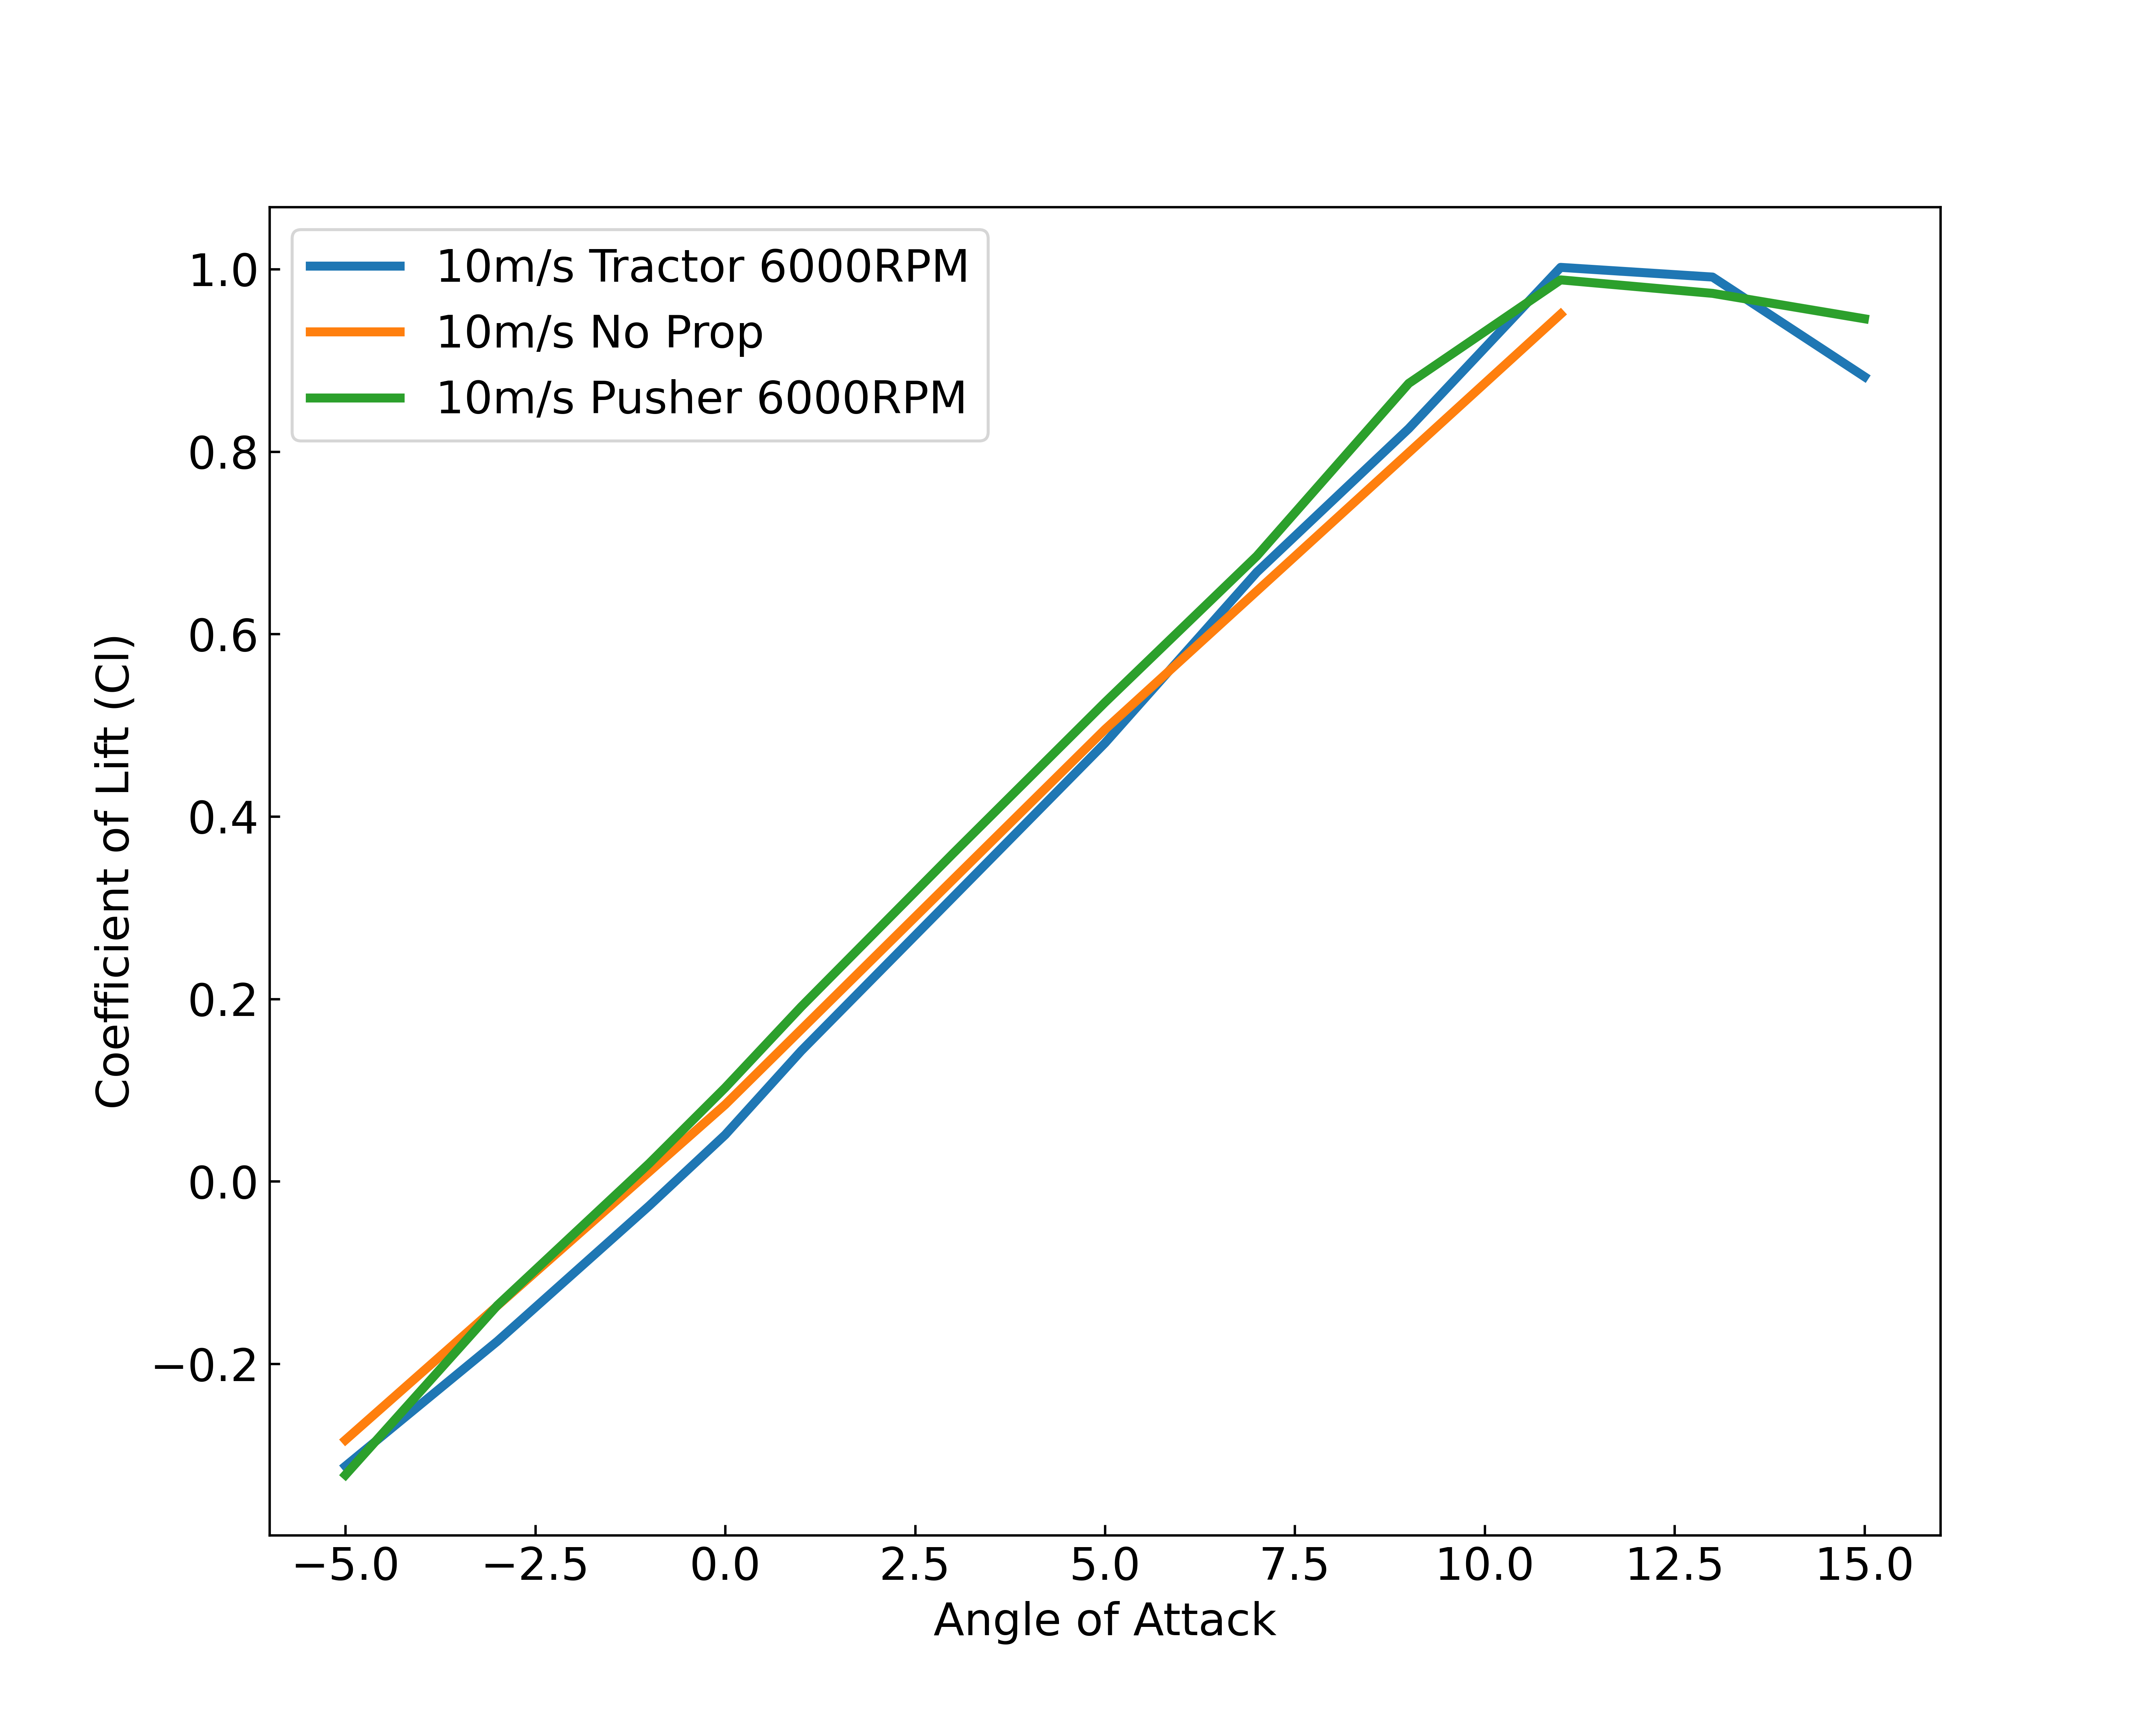
\includegraphics[width=\textwidth]{05_Results/Figs/Cl/10ms_6000RPM_Cl.png}
        \caption{Coefficient of lift at 10m/s airspeed and 6000RPM motor speed}
        \label{fig:Cl_10ms_6000}
    \end{subfigure}
    \begin{subfigure}[b]{0.467\textwidth}
        \centering
        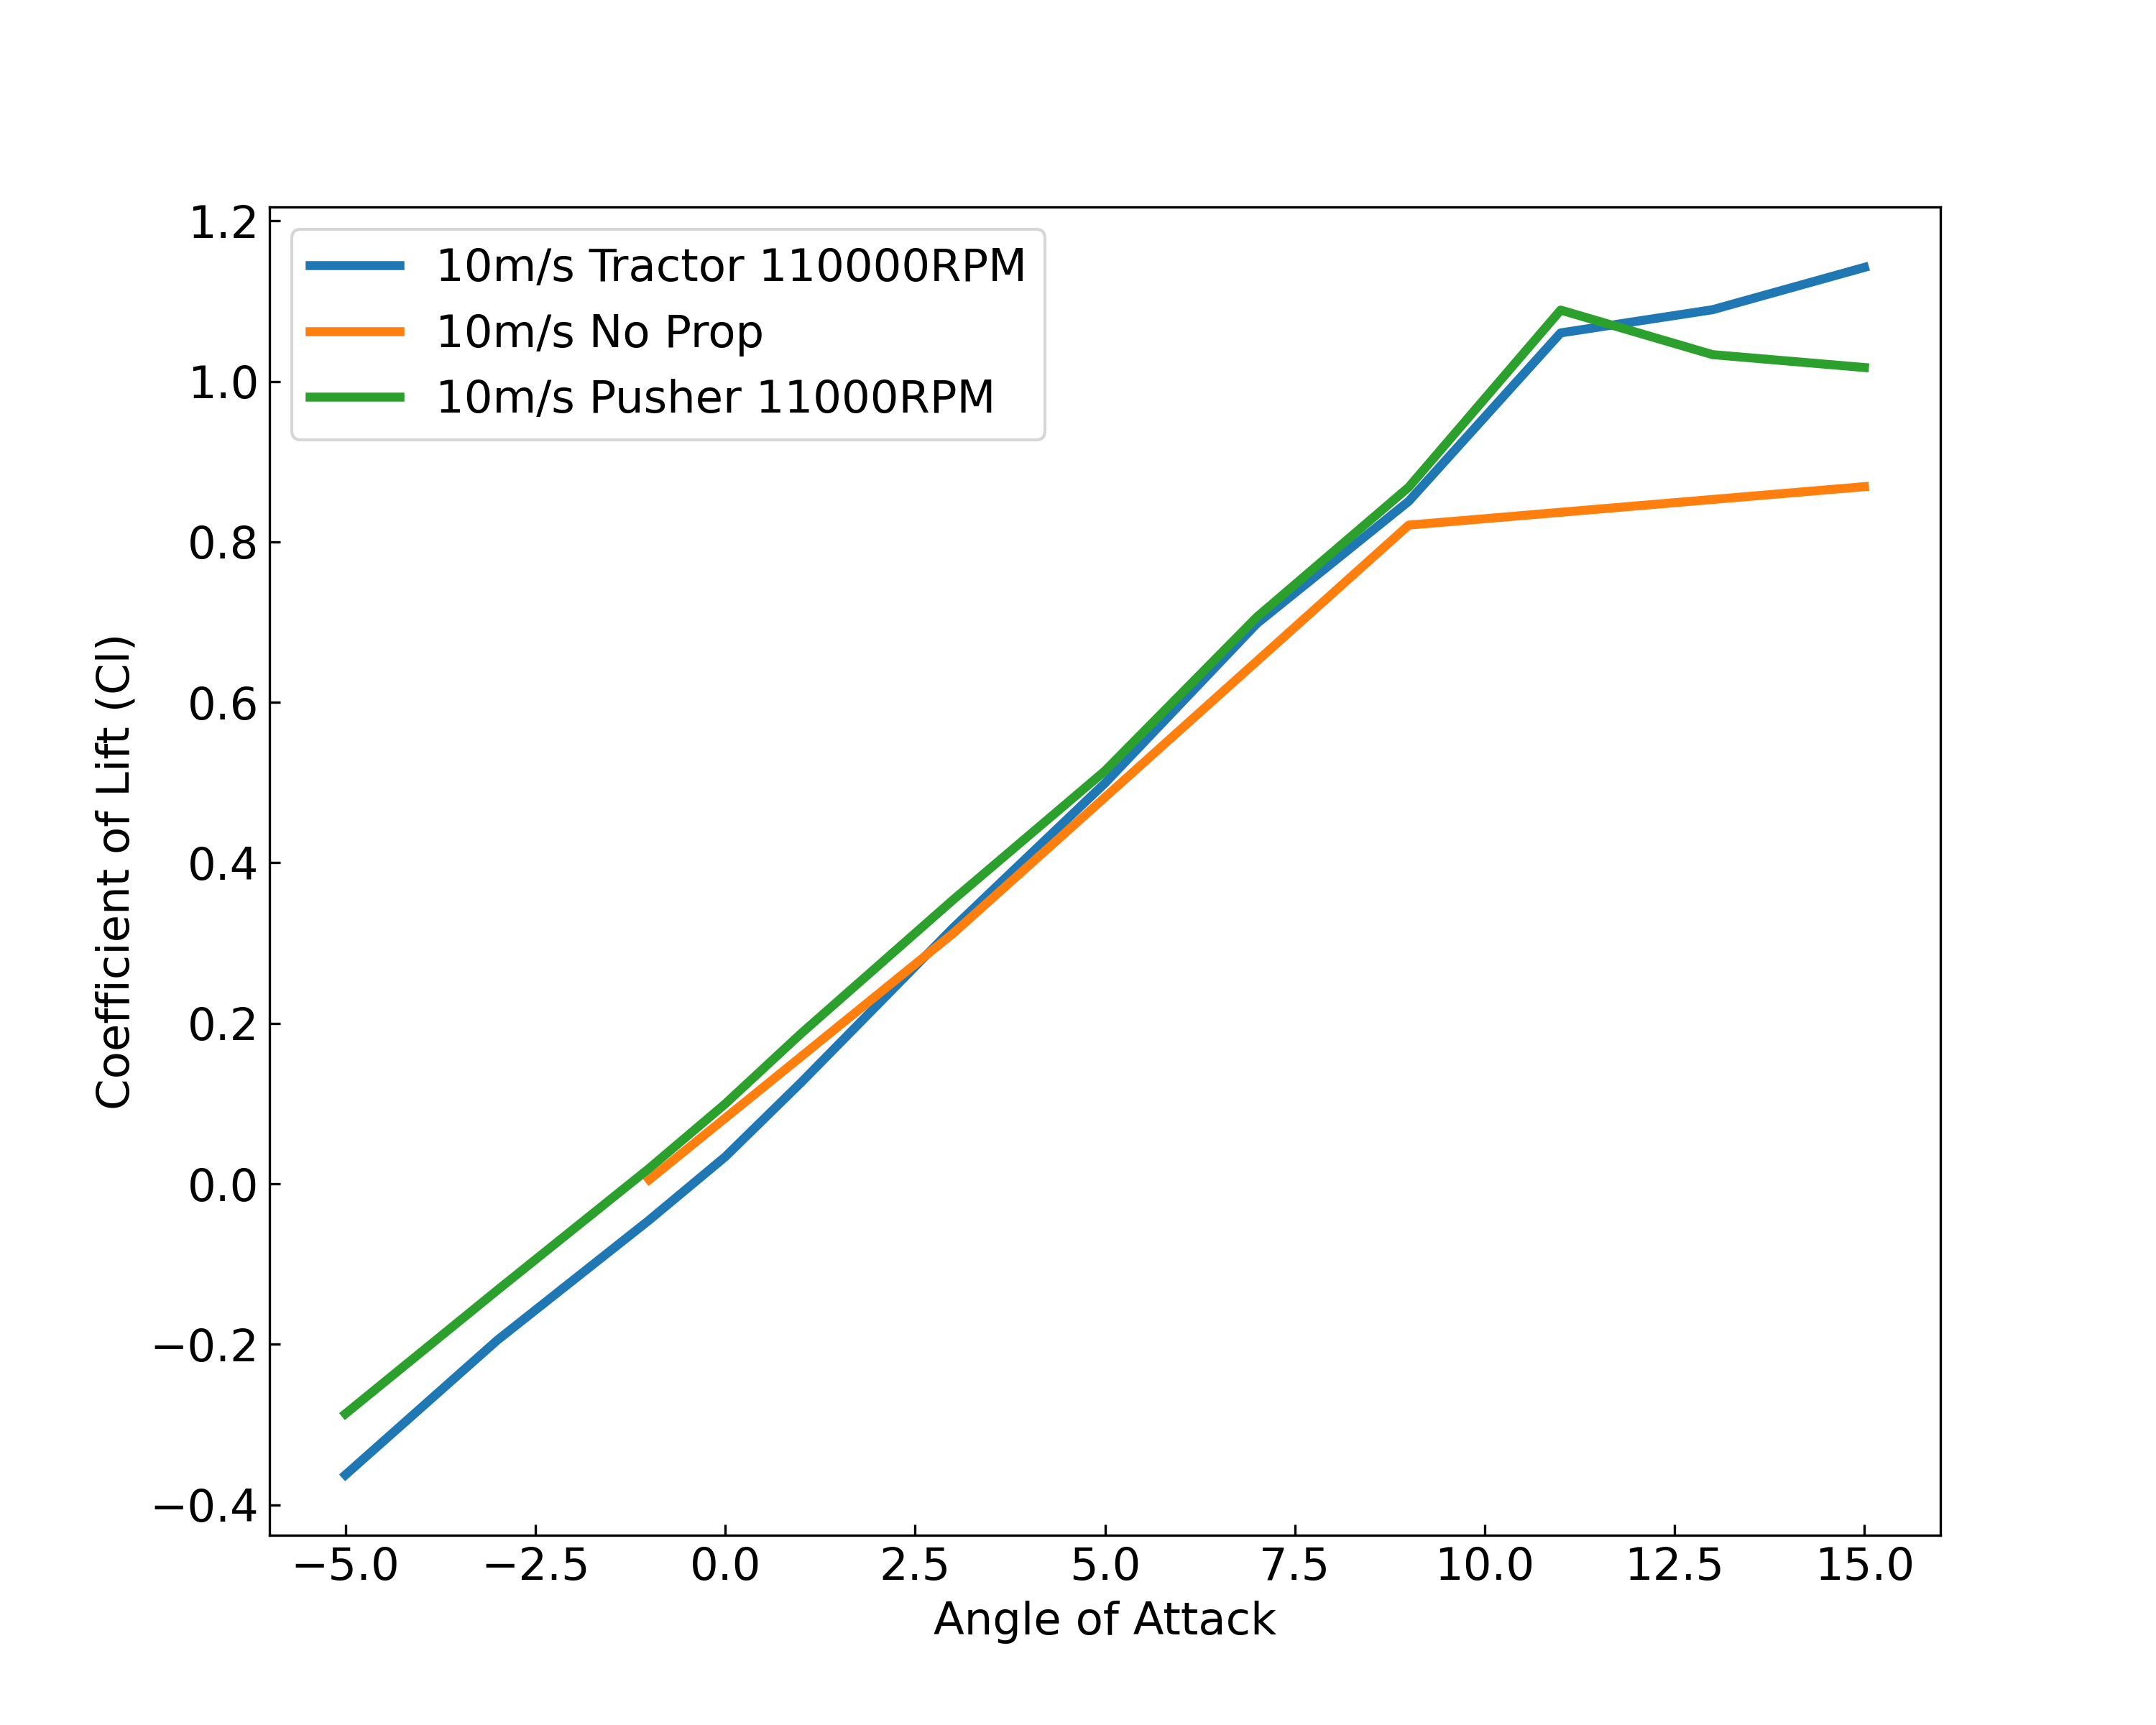
\includegraphics[width=\textwidth]{05_Results/Figs/Cl/10ms_110000RPM_Cl.png}
        \caption{Coefficient of lift at 10m/s airspeed and 11000RPM motor speed}
        \label{fig:Cl_10ms_11000}
    \end{subfigure}
    \begin{subfigure}[b]{0.467\textwidth}
        \centering
        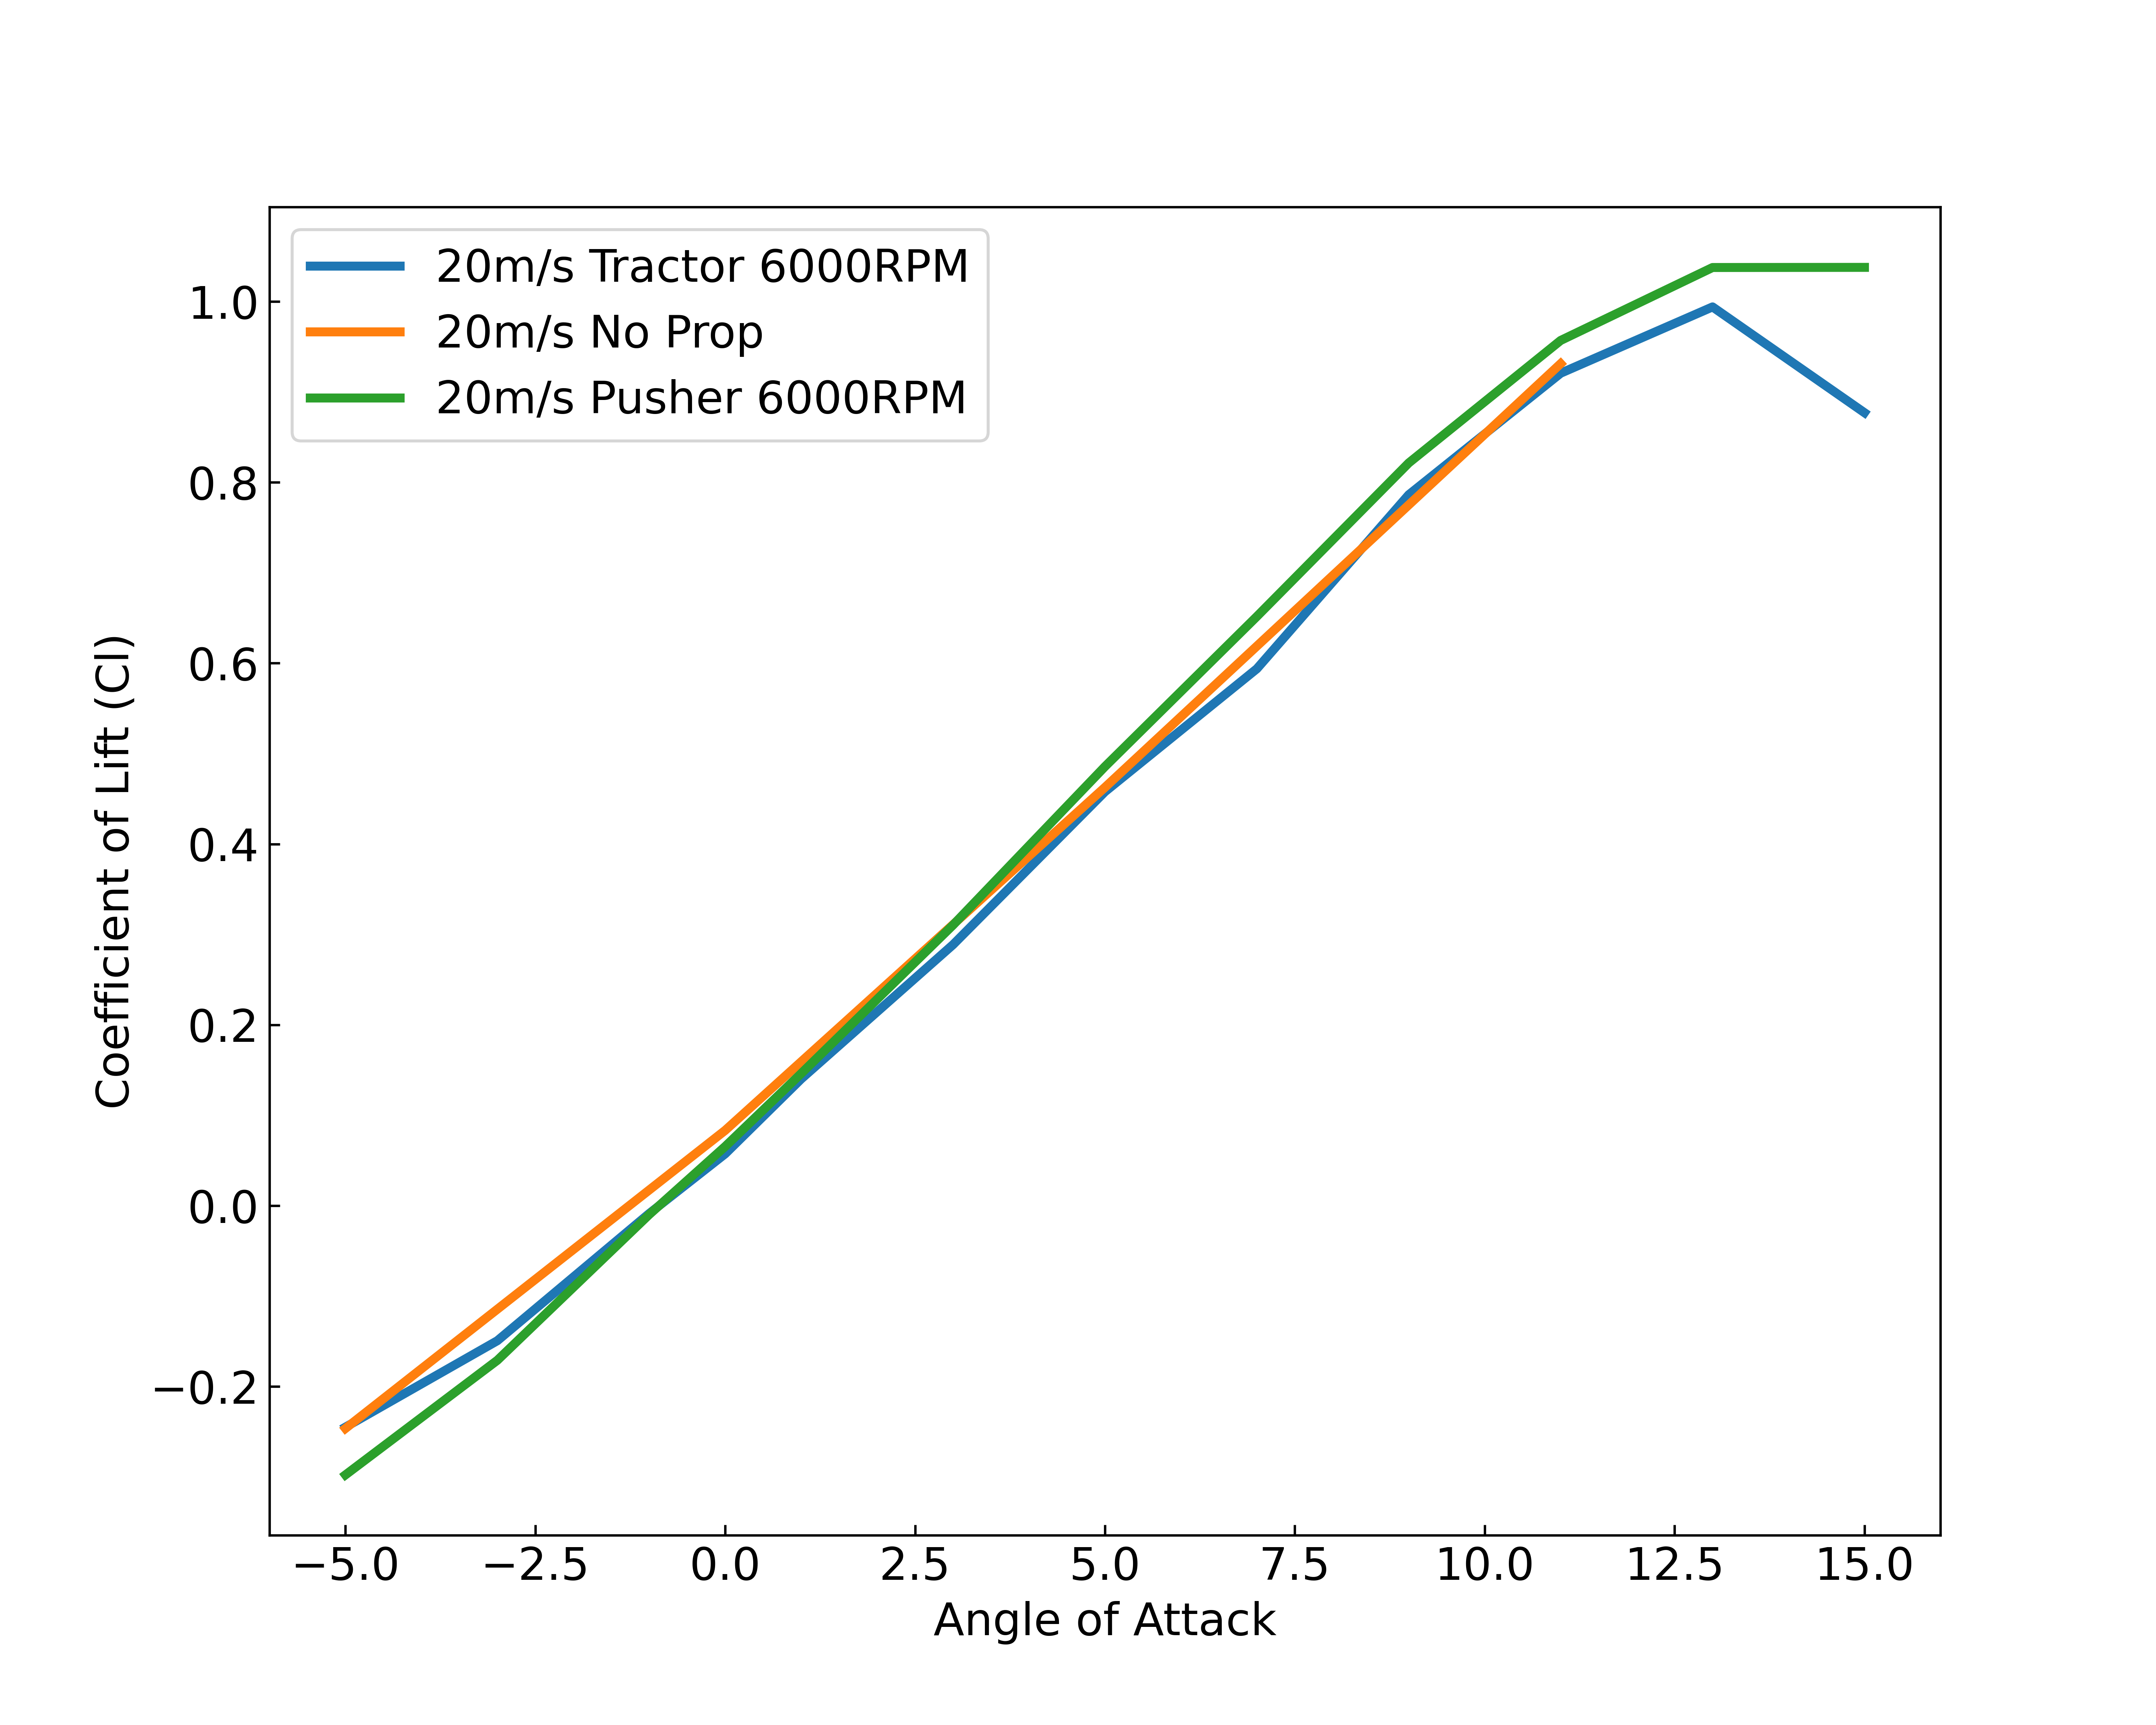
\includegraphics[width=\textwidth]{05_Results/Figs/Cl/20ms_6000RPM_Cl.png}
        \caption{Coefficient of lift at 20m/s airspeed and 6000RPM motor speed}
        \label{fig:Cl_20ms_6000}
    \end{subfigure}
    \begin{subfigure}[b]{0.467\textwidth}
        \centering
        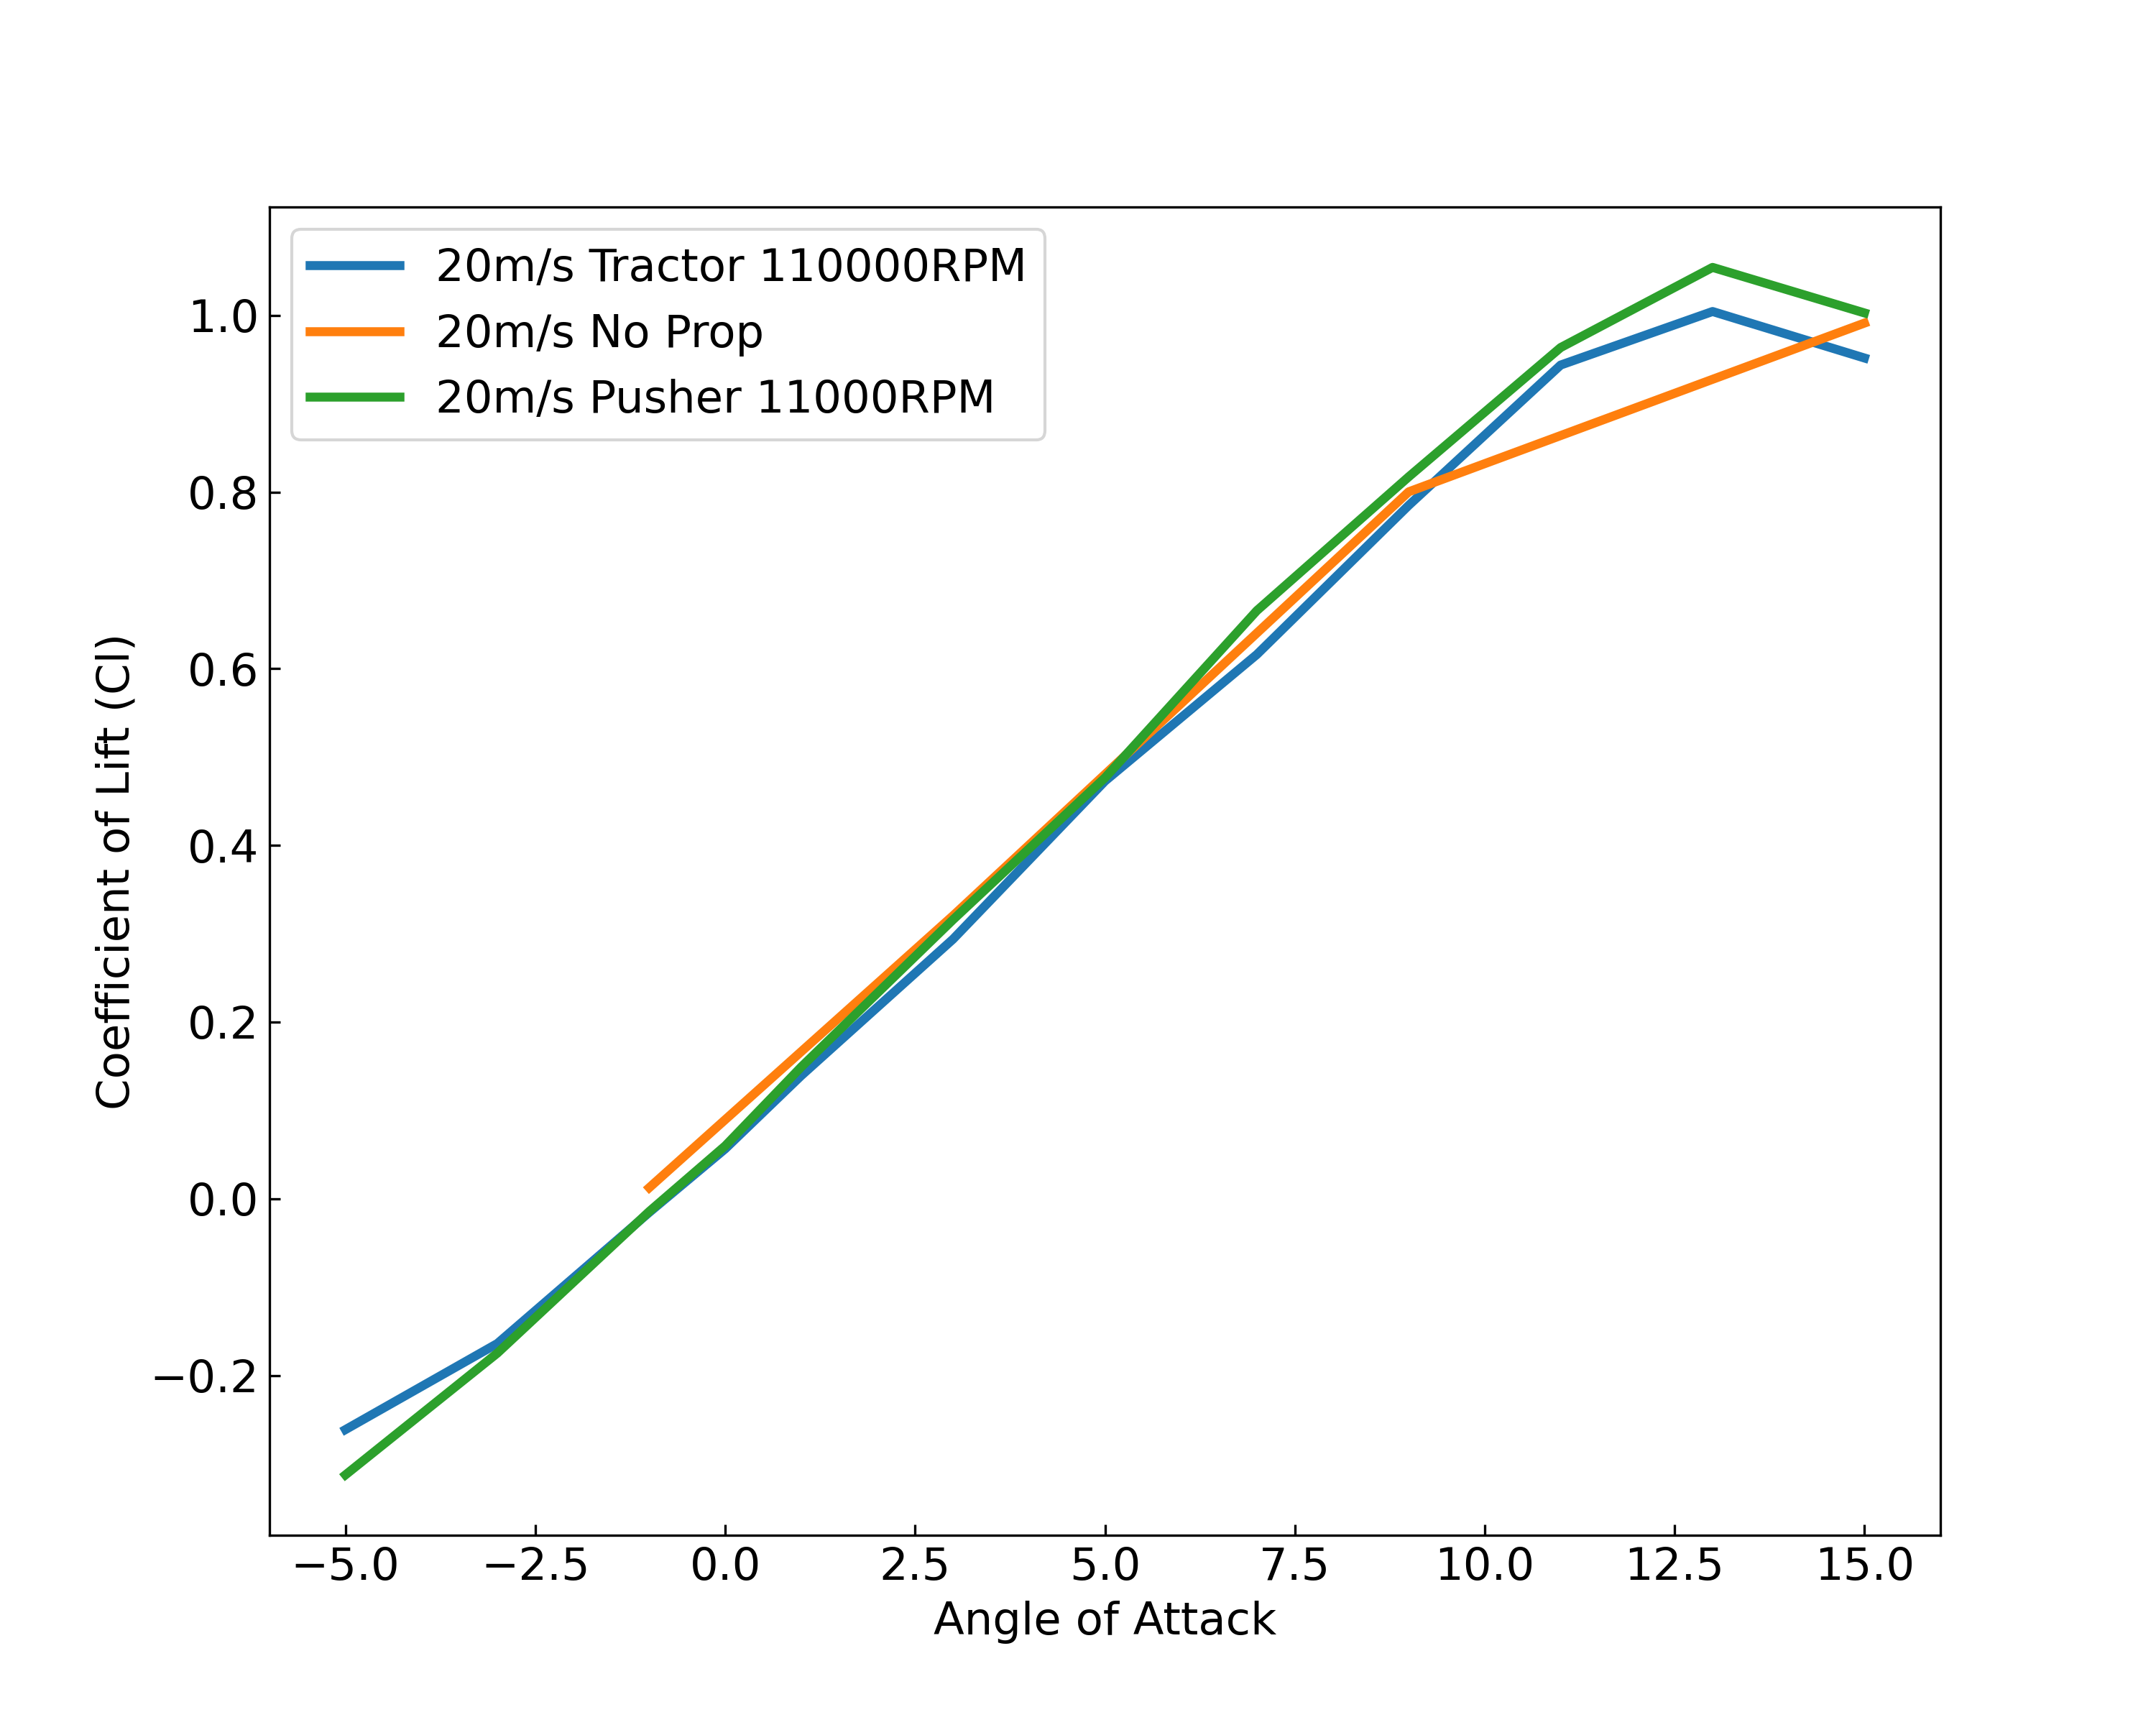
\includegraphics[width=\textwidth]{05_Results/Figs/Cl/20ms_110000RPM_Cl.png}
        \caption{Coefficient of lift at 20m/s airspeed and 11000RPM motor speed}
        \label{fig:Cl_20ms_11000}
    \end{subfigure}
    \caption{Coefficient of lift variation with various conditions for the pusher, tractor and no propeller configurations }
\end{figure}

\subsection{Aerodynamic Coefficient of Drag}
Figure \ref{fig:Cd_11000RPM} shows that as the airspeed of the wind tunnel increased the coefficient of drag shifted upwards for both the pusher and tractor configuration. The drag for both the tractor and puller configuration at 10m$s^{-1}$ airspeed is negative and shifts to positive value as the airspeed increases to 20m$s^{-1}$. This is due to the thrust produced by the propeller decreasing as the airspeed increases for both the tractor and puller configurations. The drag curve shifts into negative values for the tractor and puller configurations due to the thrust produced by the propeller. As the overall drag which is a measure of the thrust minus drag, the overall drag becomes negative, shifting the coefficient of drag curve into negative values. As the airspeed increases the coefficient of drag is also seen to increase for the pusher and tractor configuration due to an increase in drag for the overall model with increasing airspeed. This shifts the coefficeint of drag curves upwards as the airspeed increases.  The highest coefficient of drag is seen when no propeller is operating on the MAV model. When no propeller is added, no significant changes are seen with airspeed for the coefficient of drag. The tractor configuration in general produces less drag compared with the pusher configuration and hence the overall drag seen in the coefficient of drag is larger for the pusher configuration, this is most clearly seen at 20m$s^{-1}$ in Figure \ref{fig:Cd_11000RPM}. 
\todo{change line style here \& remove extra noProp lines}

\begin{figure}[H]
    \centering
    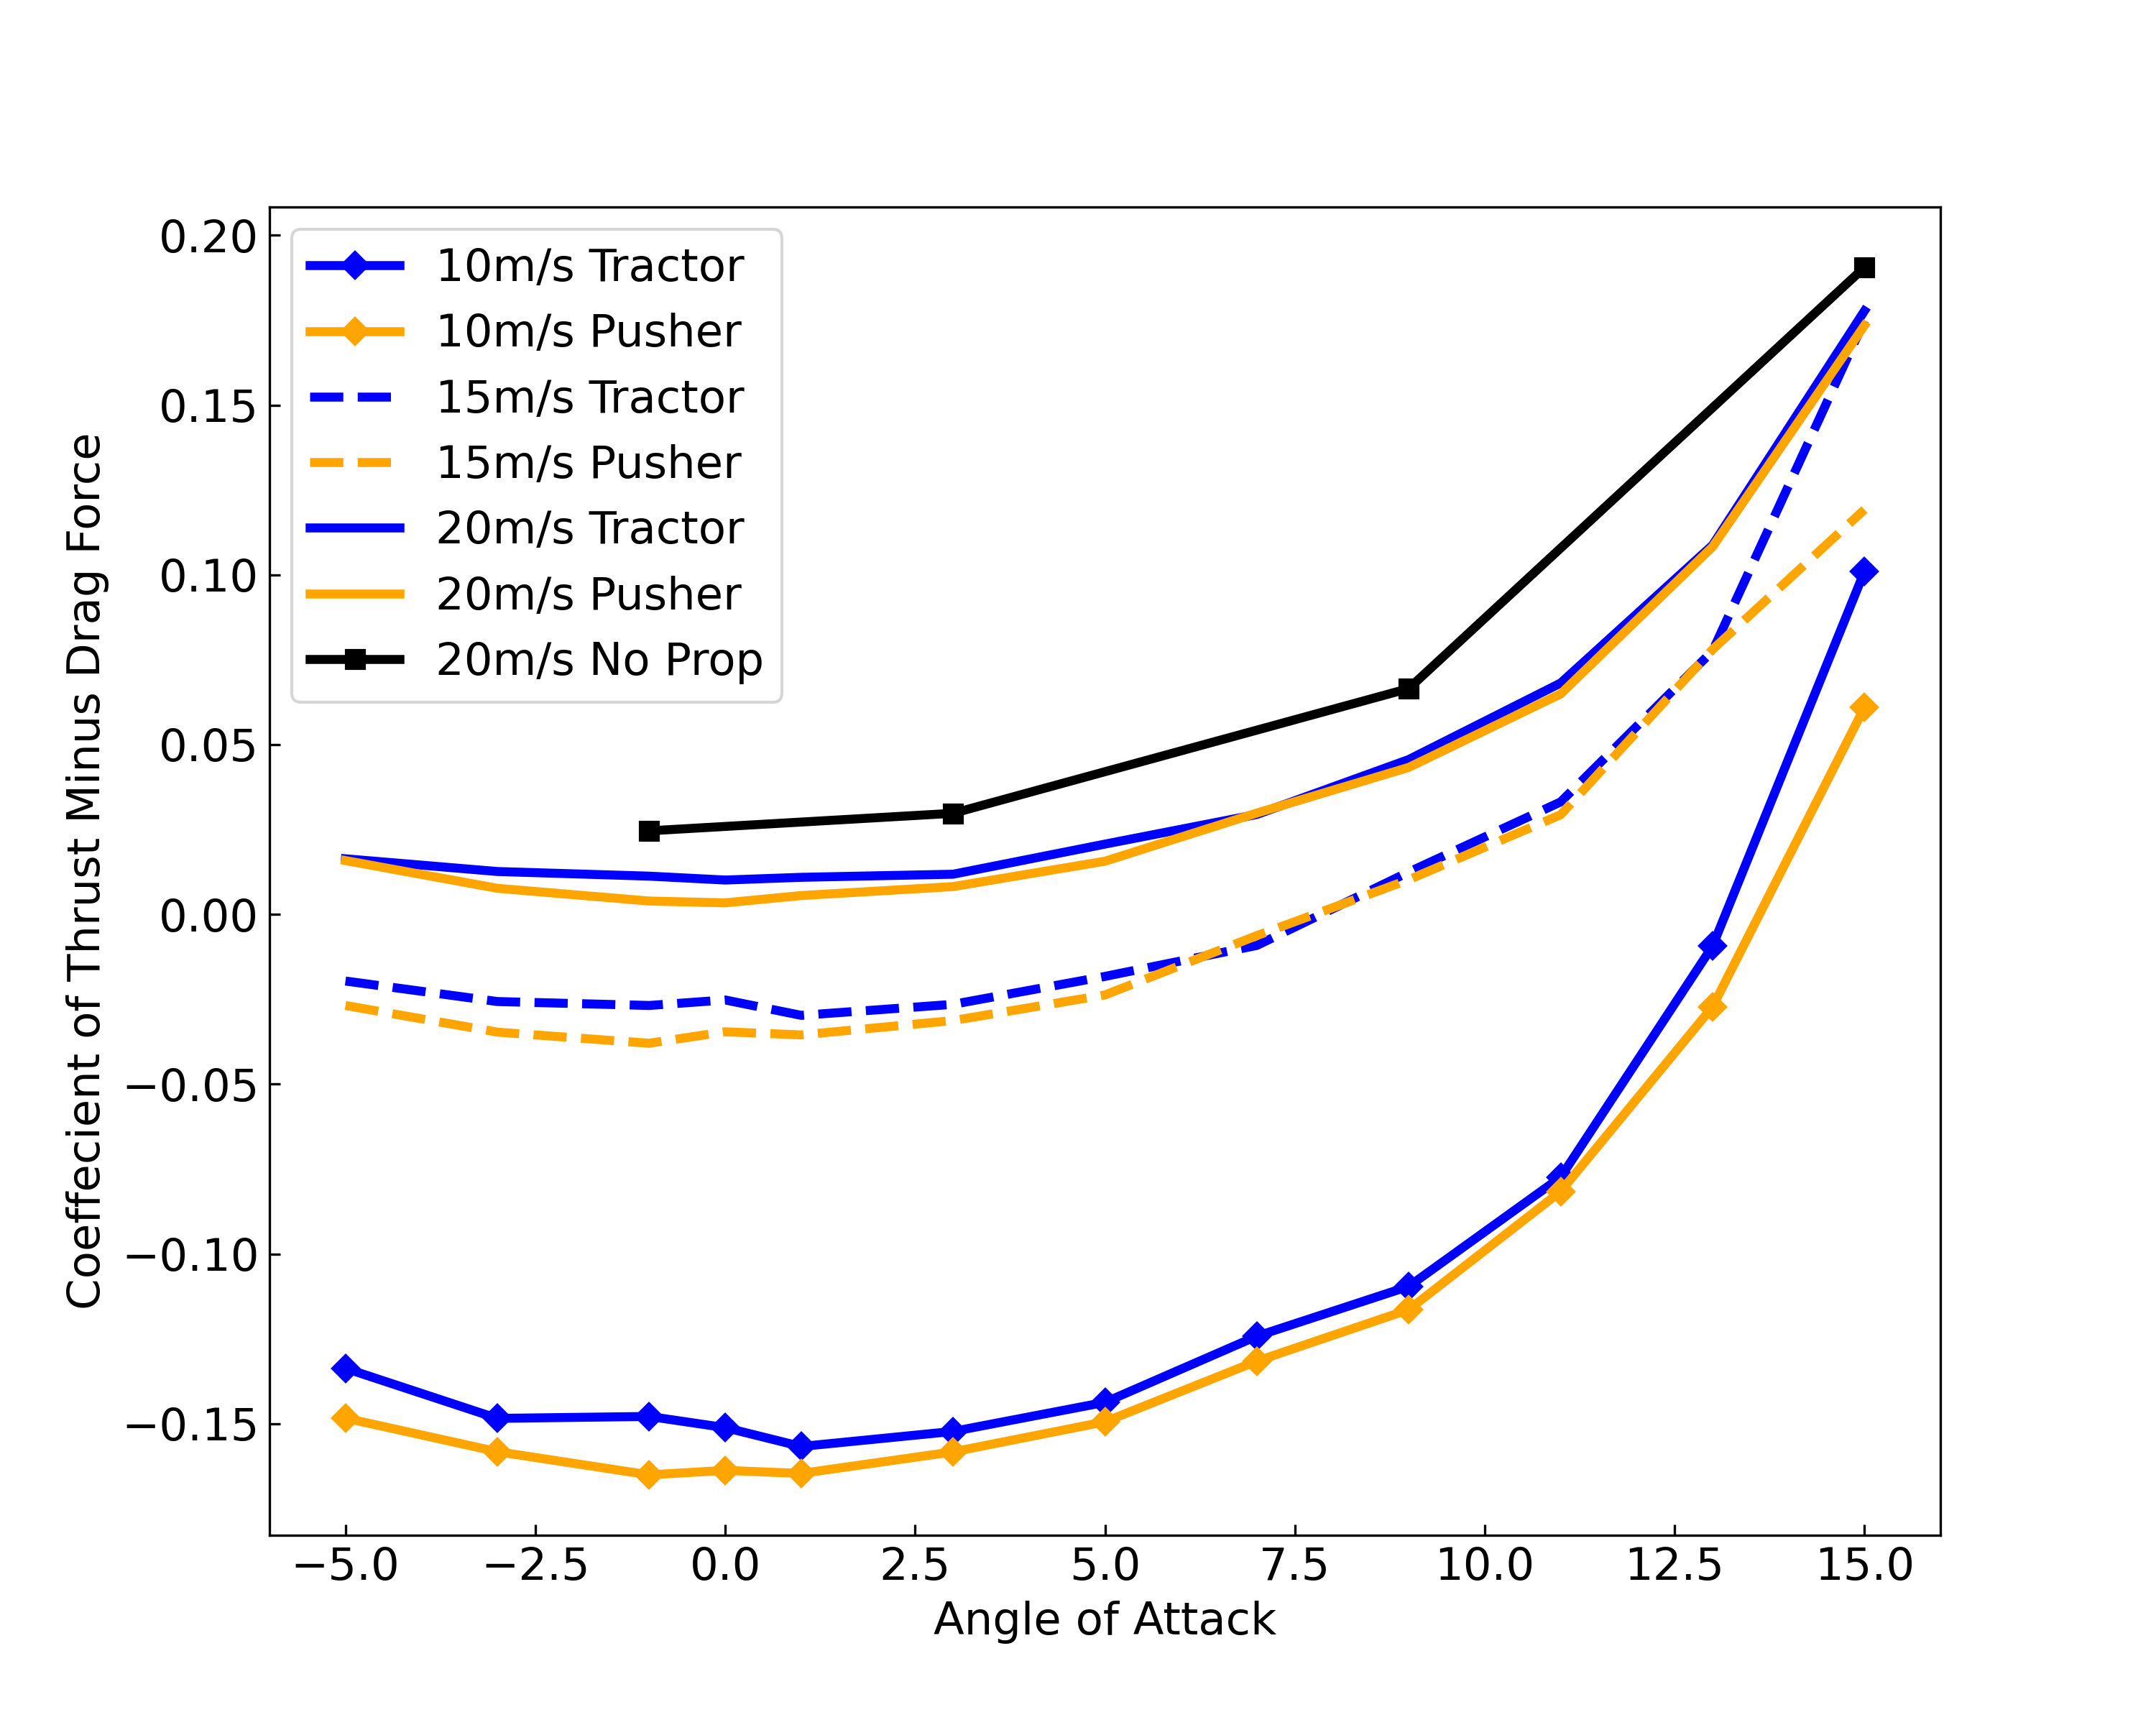
\includegraphics[scale = 0.7]{05_Results/Figs/Cd/110000RPM_Cd.png}
    \caption{Coefficient of drag variation at 11000RPM motor speed for the tractor, pusher and no propeller configurations}
    \label{fig:Cd_11000RPM}
\end{figure}

Figure \ref{fig:Cd_20ms} shows minimal differences between the pusher and tractor configurations. The addition of the propeller increases the coefficient of drag at 6000RPM. This shows that the propellers do not produce enough thrust to overcome the drag at 20m$s^{-1}$. As the motor speed increases to 11000RPM there is a significant drop in the coefficient of drag for both the tractor and pusher configuration, showing that the thrust produced is able to overcome drag at 11000RPM. 
\todo{get rid of extra no prop lines - keep one only}
\begin{figure}[H]
    \centering
    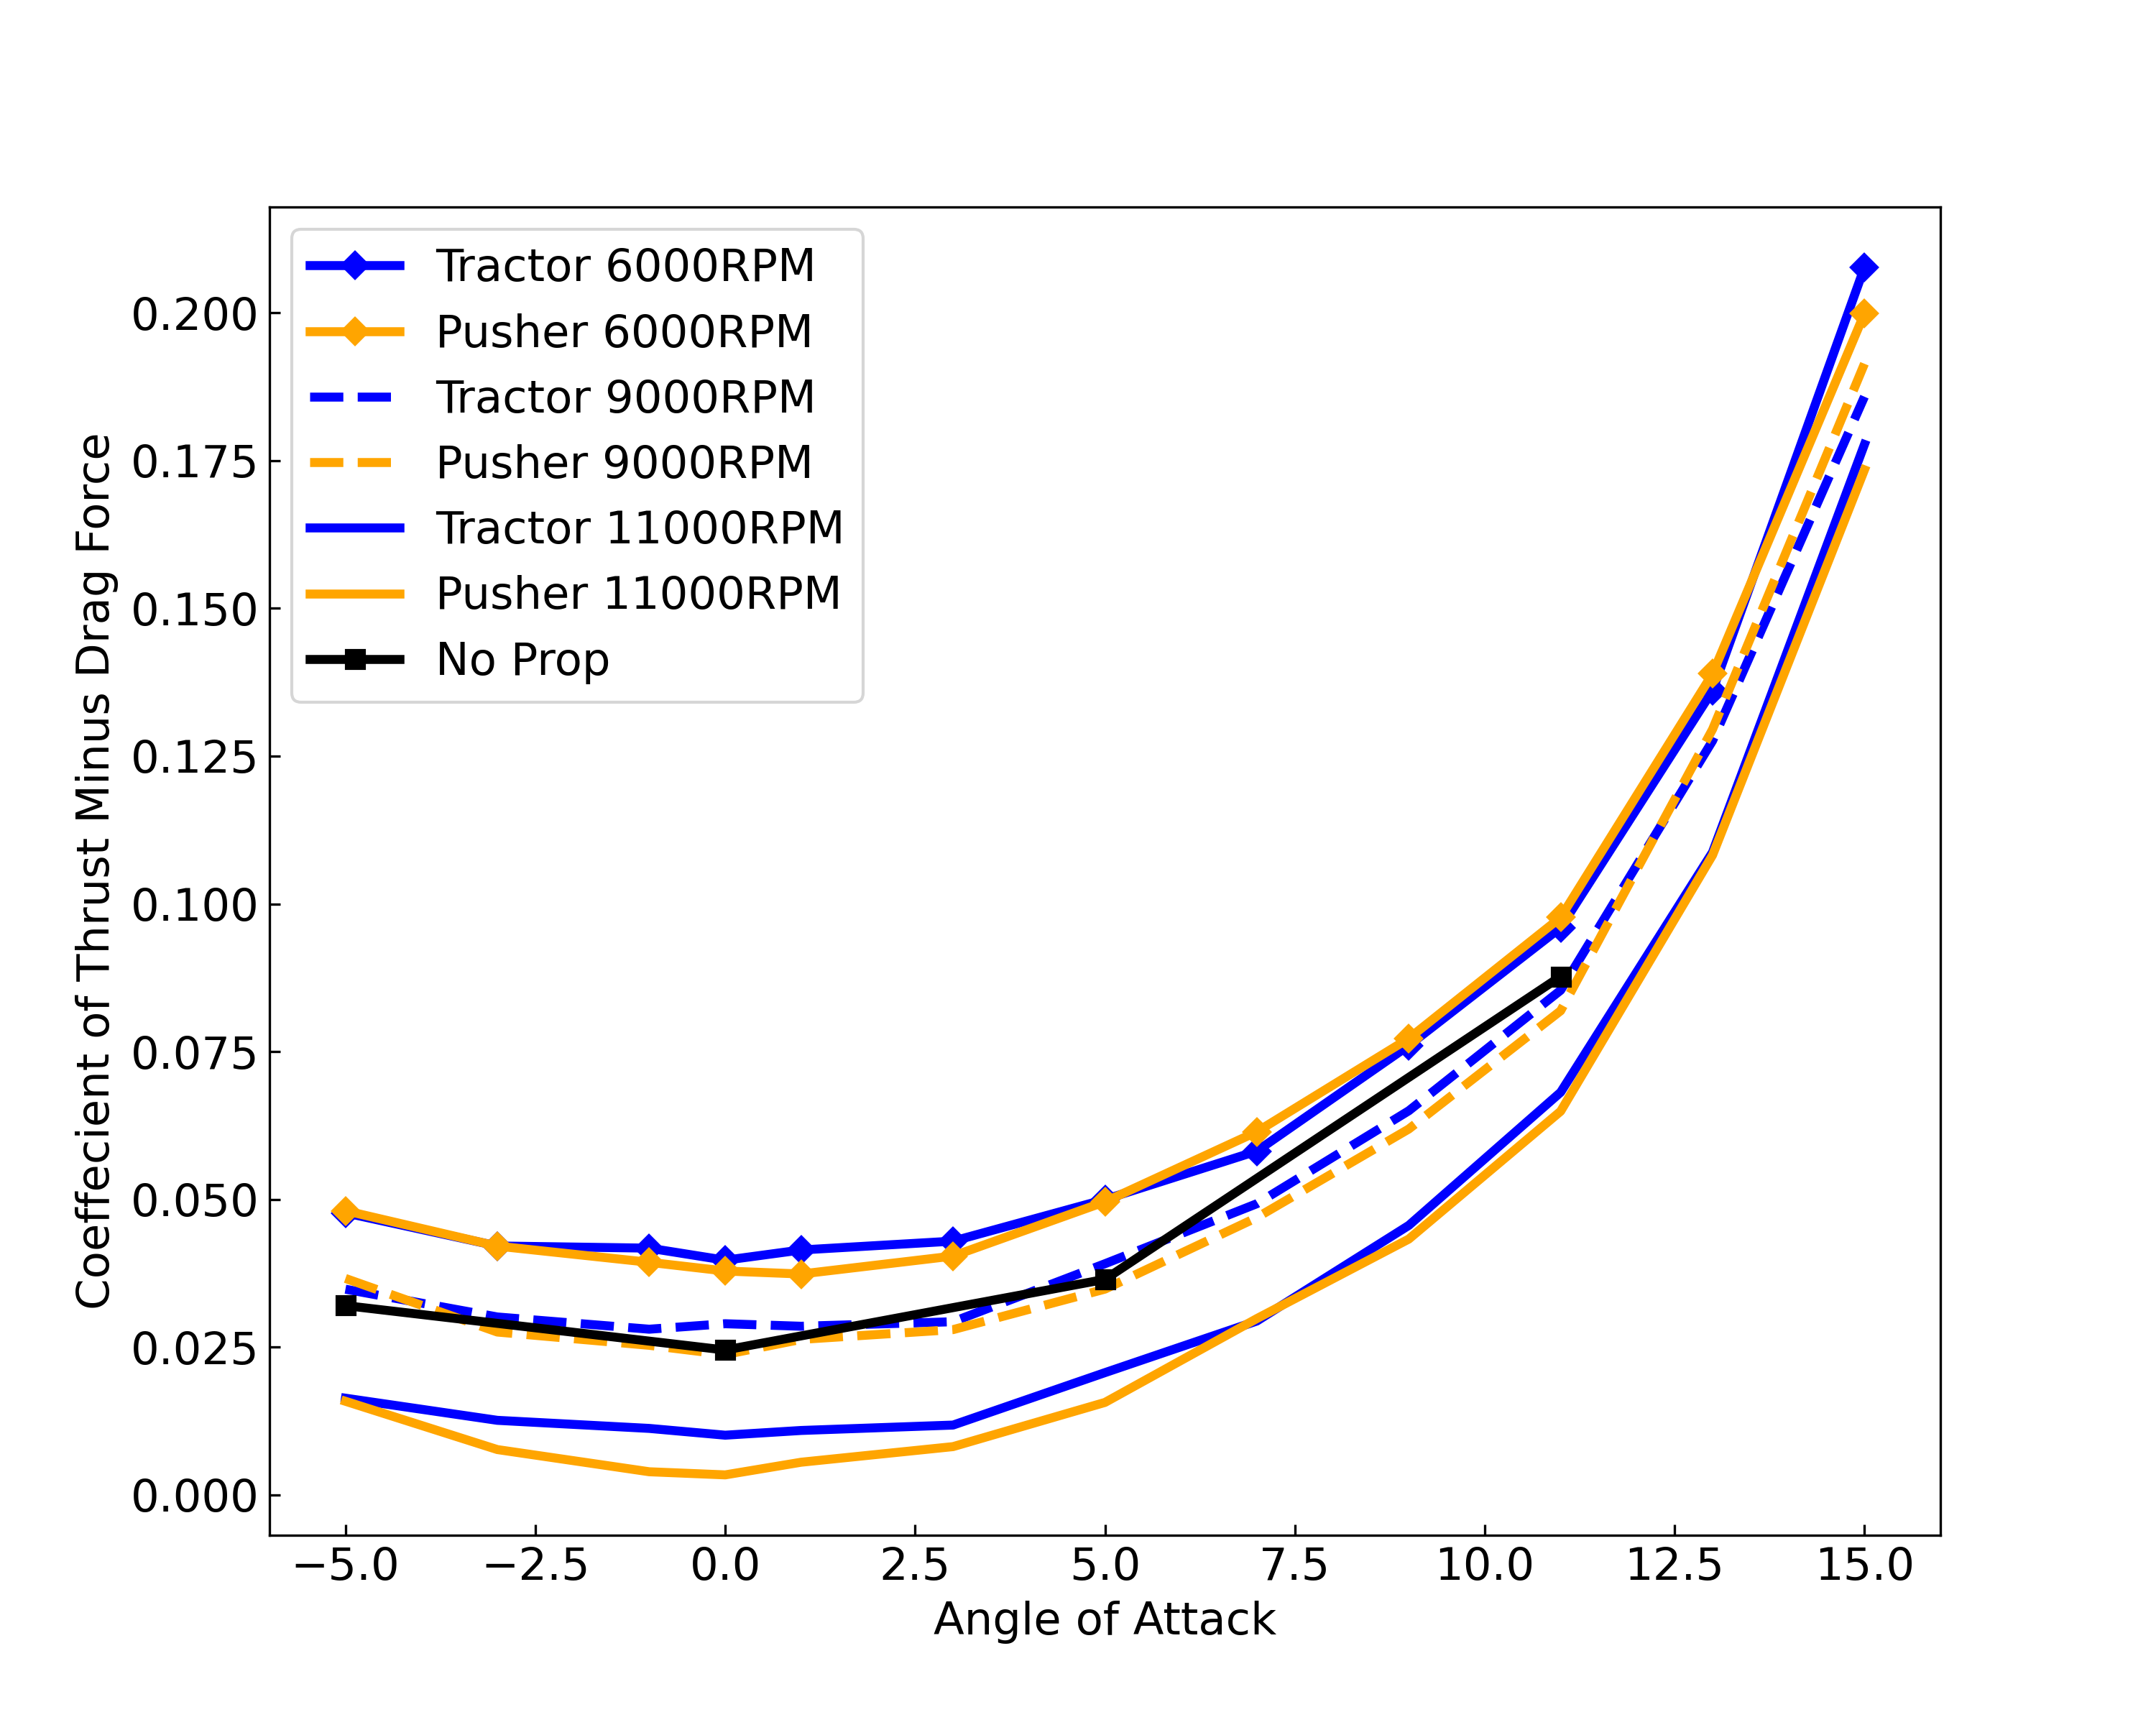
\includegraphics[scale = 0.7]{05_Results/Figs/Cd/20ms_Cd.png}
    \caption{Coefficient of drag variation at 20ms airspeed for the tractor, pusher and no propeller configuration}
    \label{fig:Cd_20ms}
\end{figure}

\subsection{Pitching Moment Coefficient}

Figure \ref{fig:Cm_graphs} shows that as the motor speed increases from 6000RPM to 11000RPM the tractor configuration experienced a decrease in pitching coefficient compared with the no propeller model up until stall at approximately 12$^\circ$ AoA. The pusher configration experienced an increase in the pitching moment compared with the no propeller model. Increasing the airspeed decreased the pitching moment for all motor speeds.

\begin{figure}[H]
    \centering
    \begin{subfigure}[b]{0.467\textwidth}
        \centering
        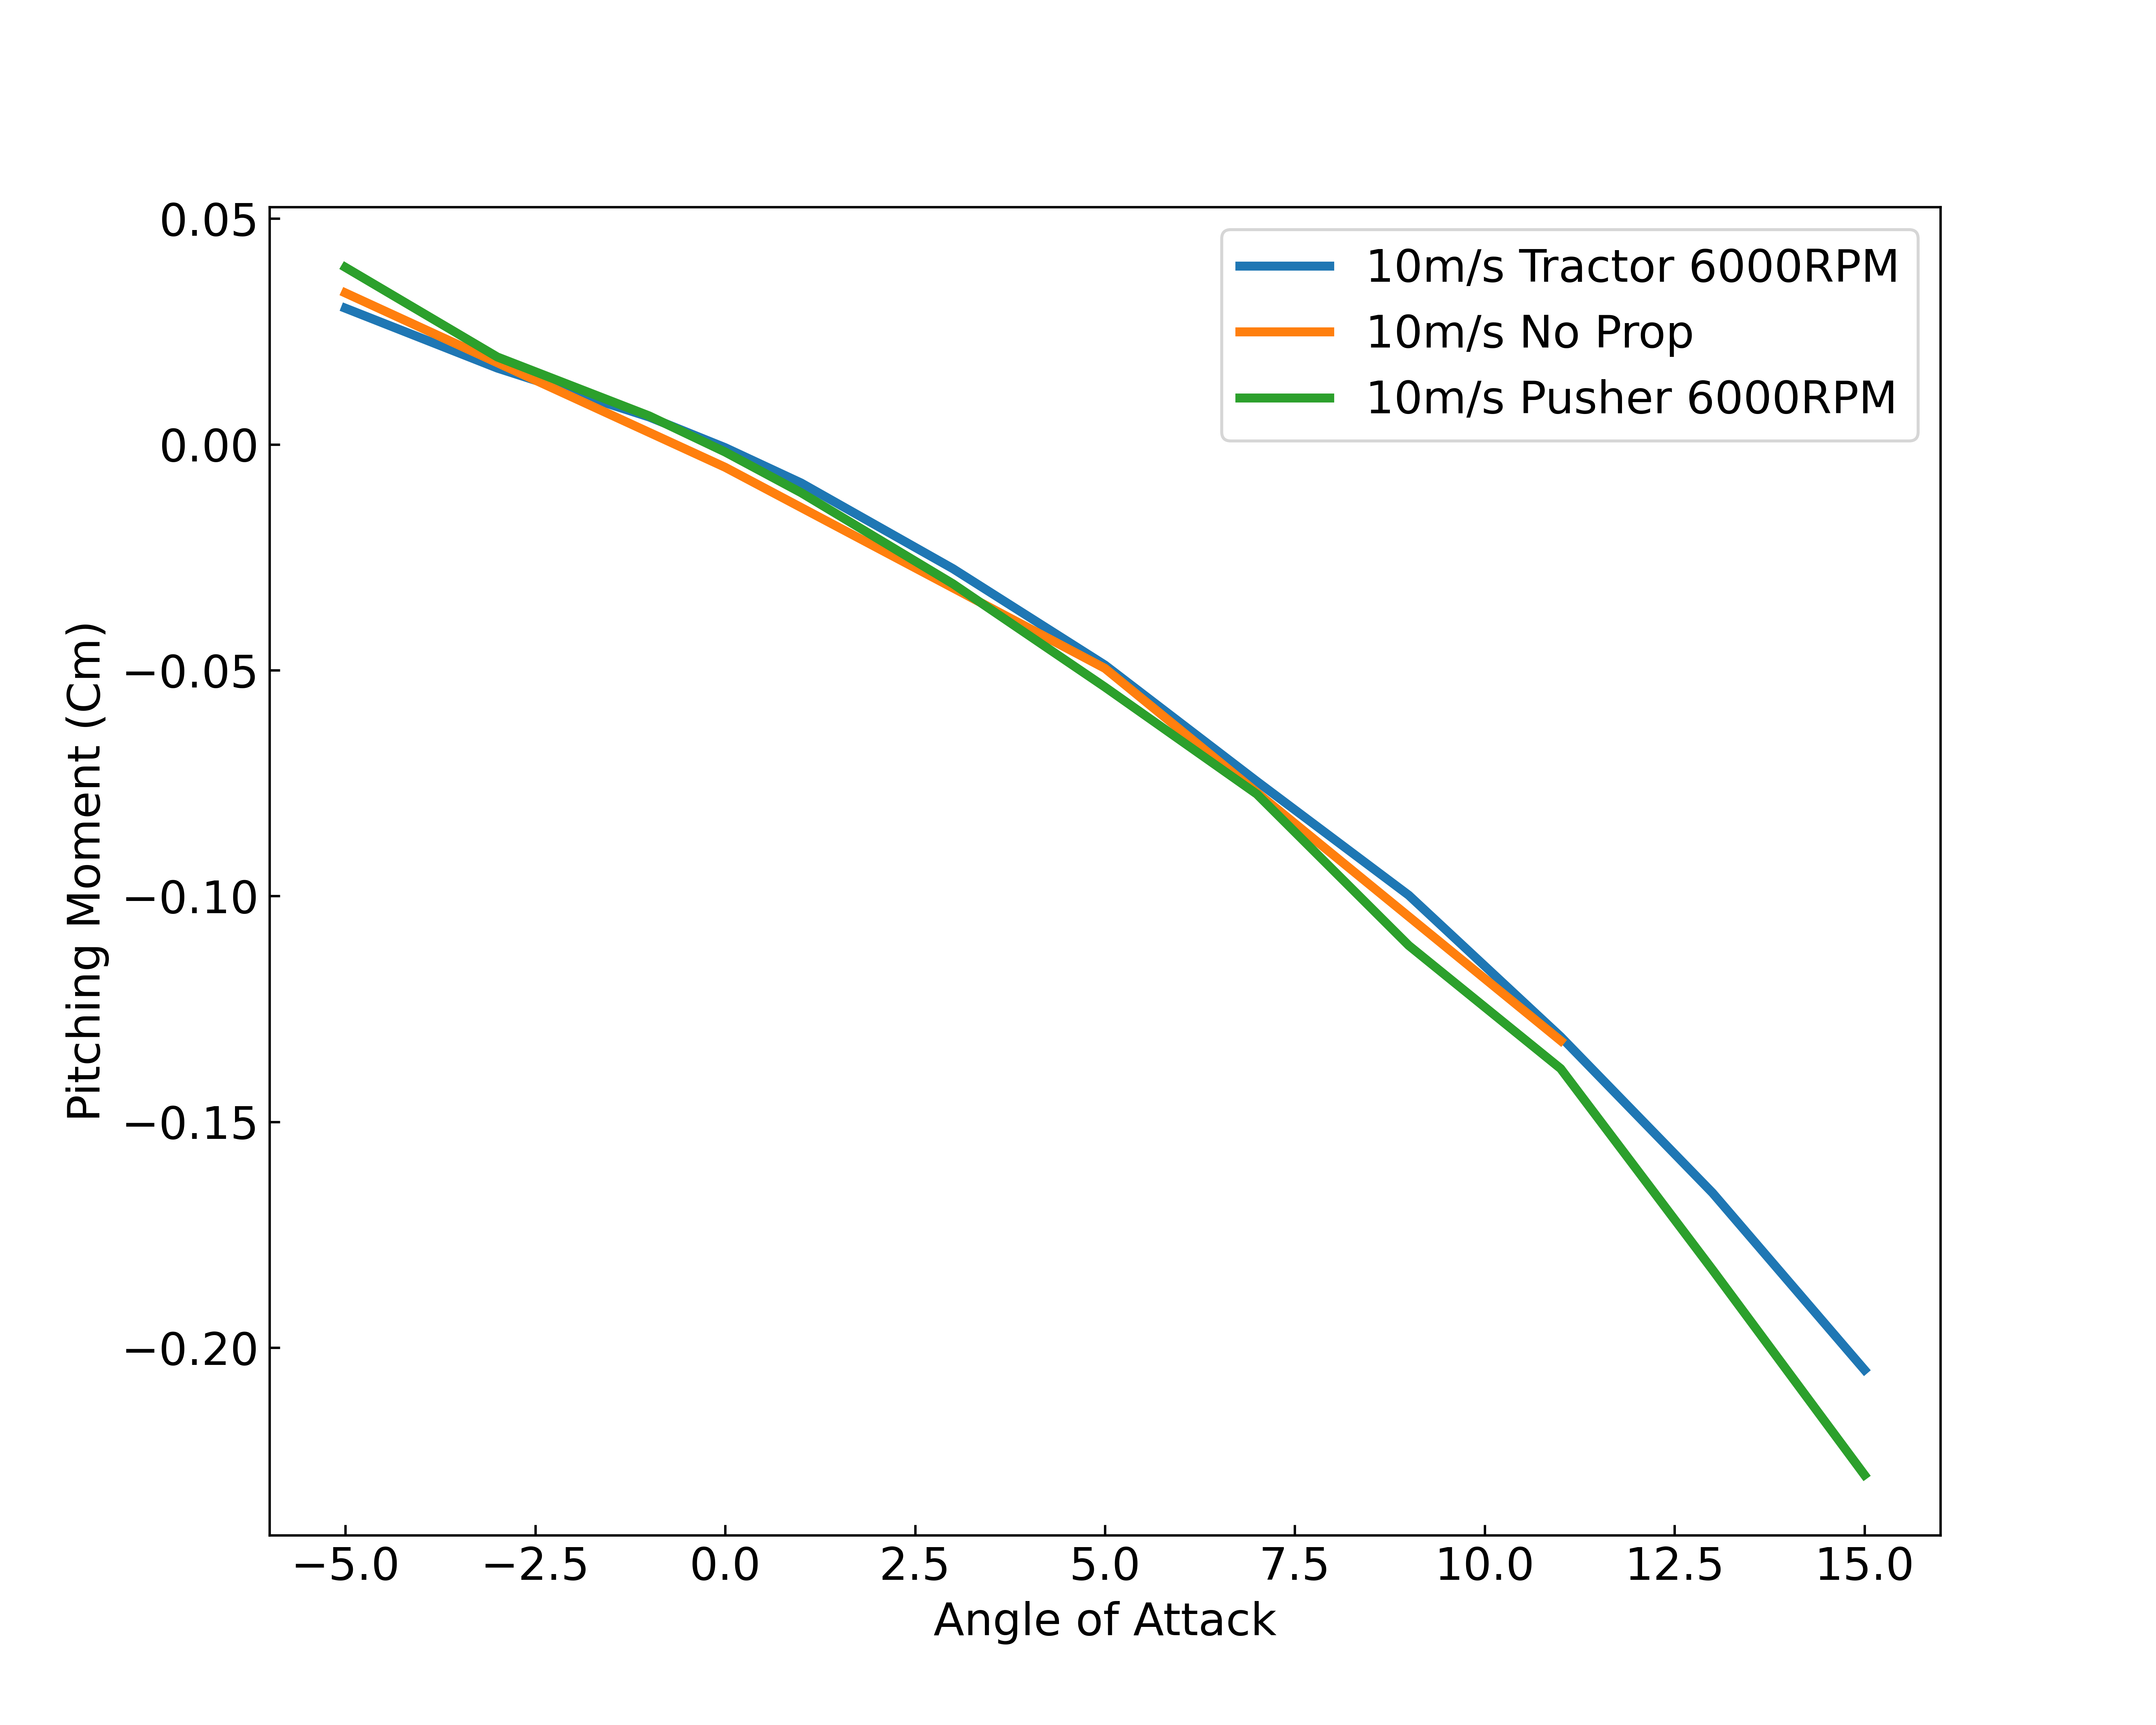
\includegraphics[width=\textwidth]{05_Results/Figs/Cm/10ms_6000RPM_Cm.png}
        \caption{Pitching Moment Coefficient at 10m/s airspeed and 6000RPM motor speed}
        \label{fig:Cm_10ms_6000}
    \end{subfigure}
    \begin{subfigure}[b]{0.467\textwidth}
        \centering
        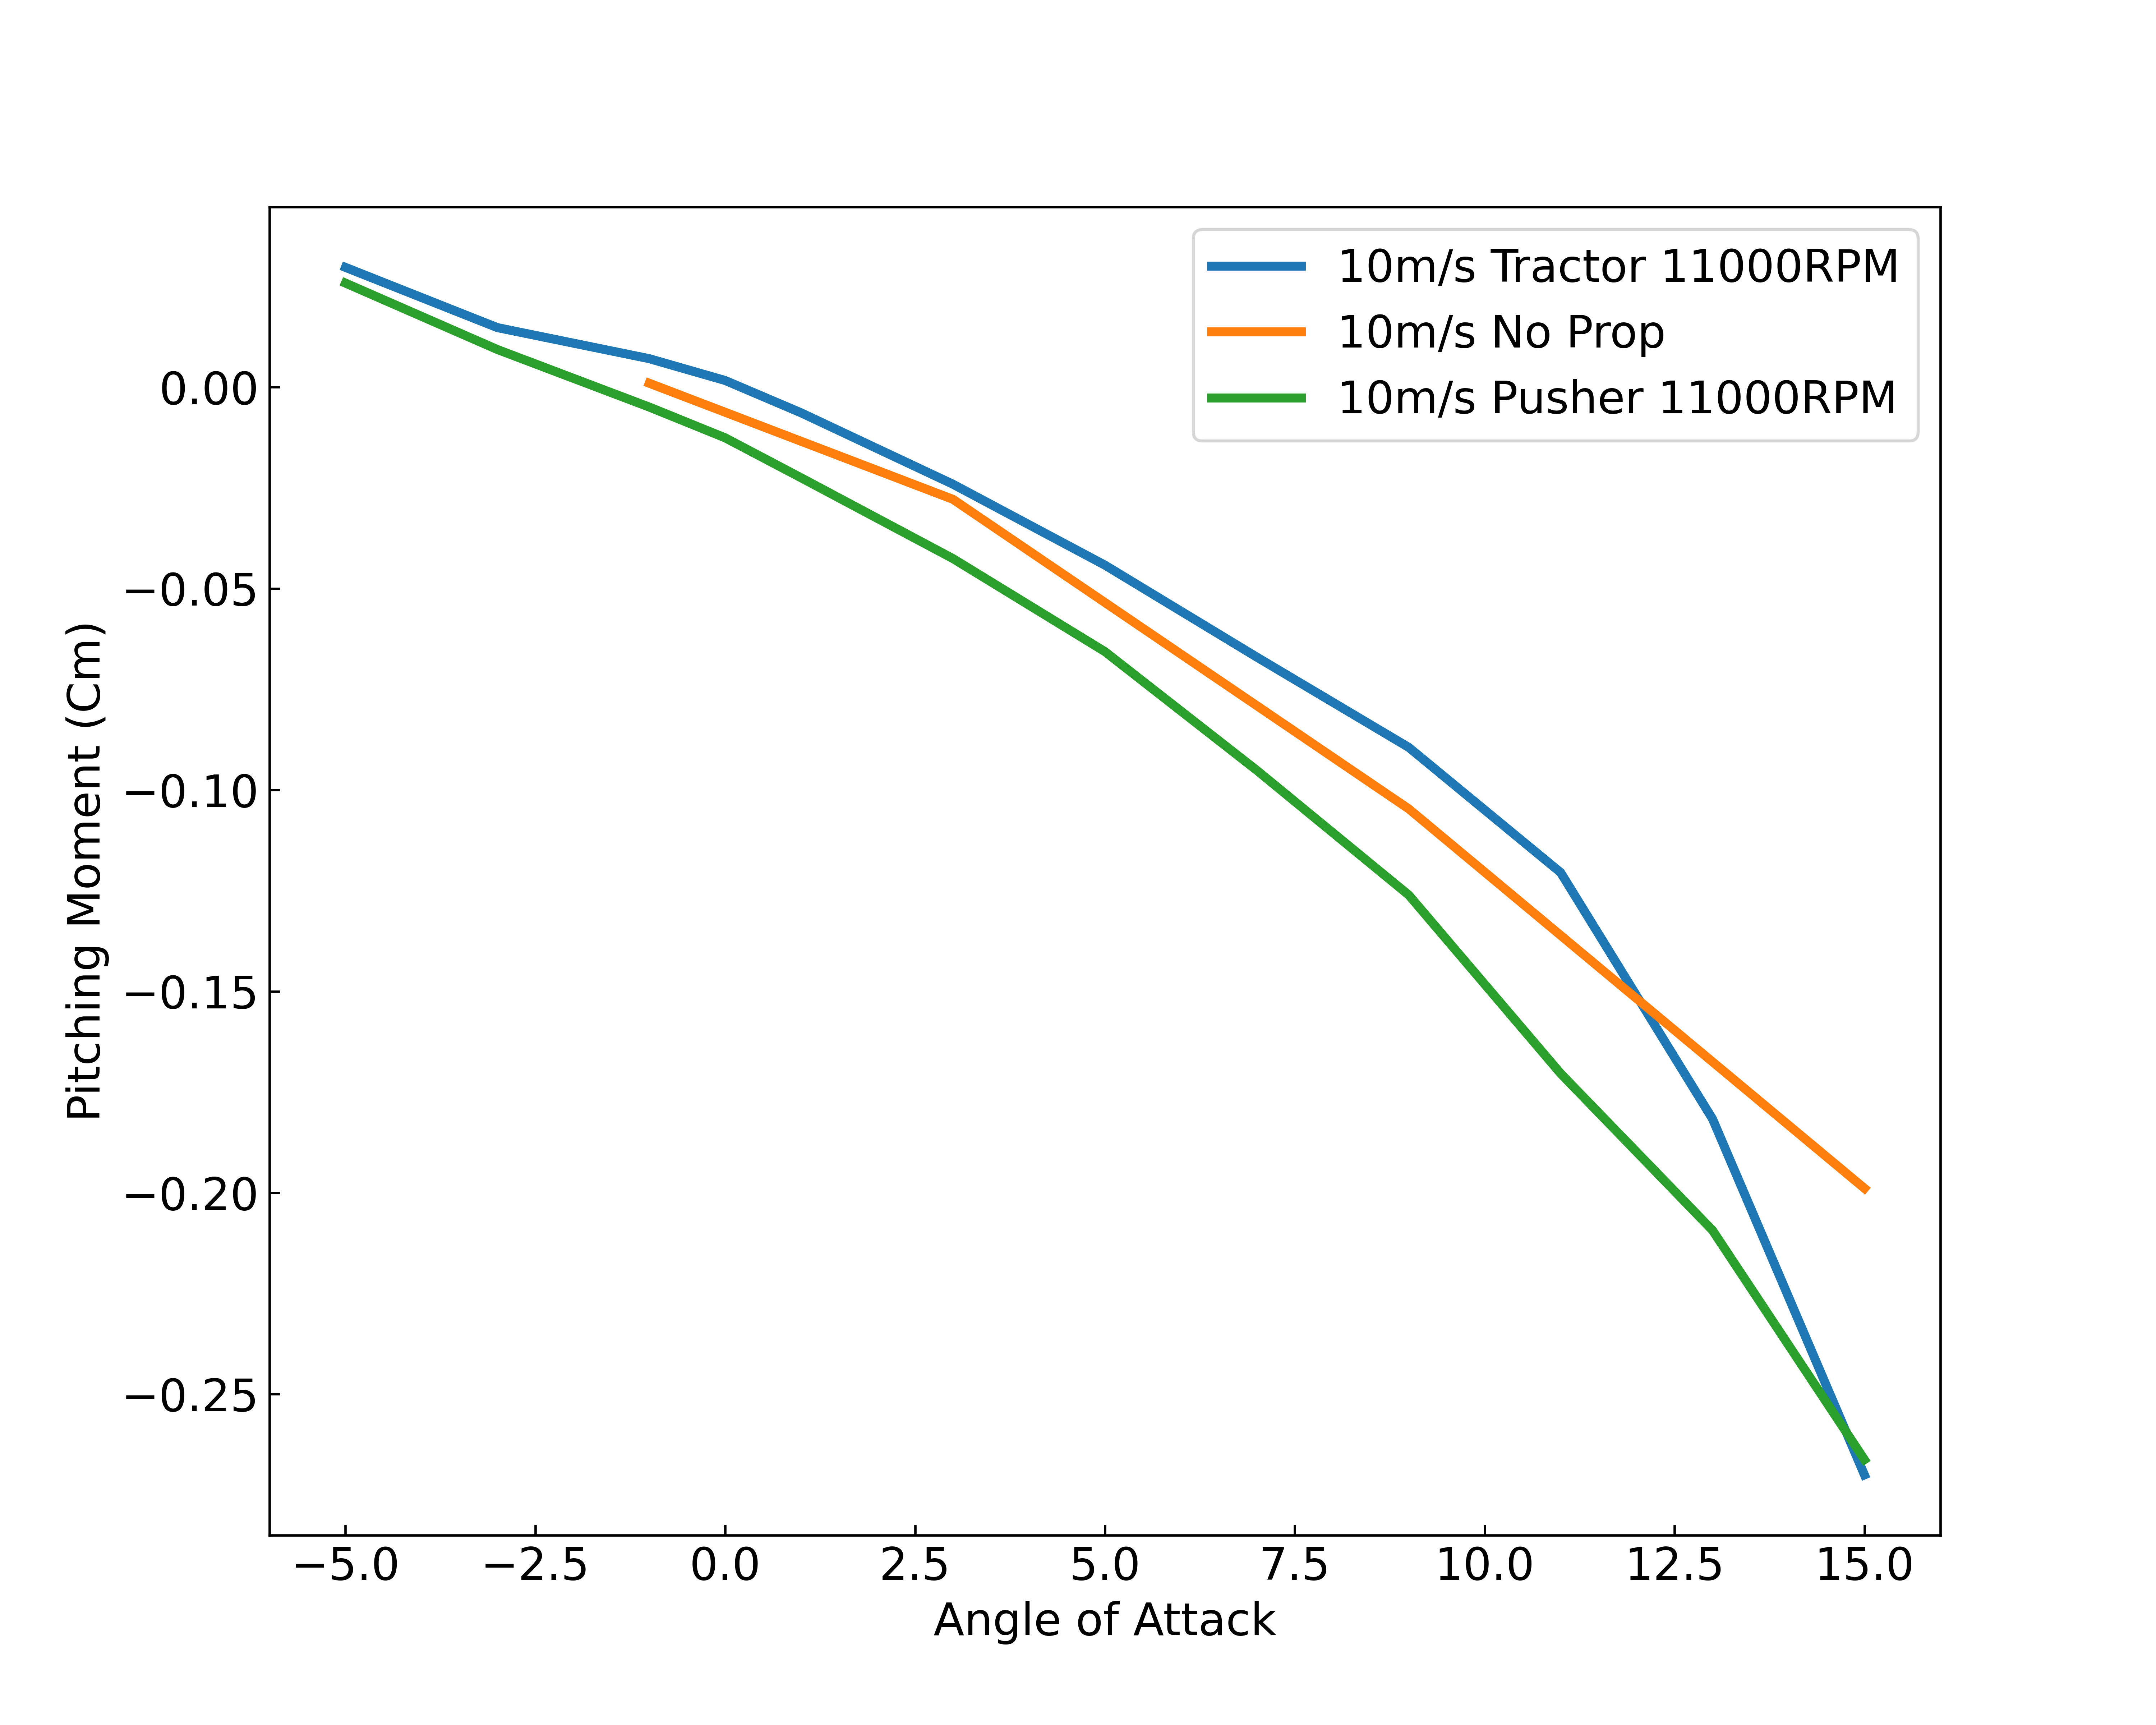
\includegraphics[width=\textwidth]{05_Results/Figs/Cm/10ms_11000RPM_Cm.png}
        \caption{Pitching Moment Coefficient at 10m/s airspeed and 11000RPM motor speed}
        \label{fig:Cm_10ms_11000}
    \end{subfigure}
    \begin{subfigure}[b]{0.467\textwidth}
        \centering
        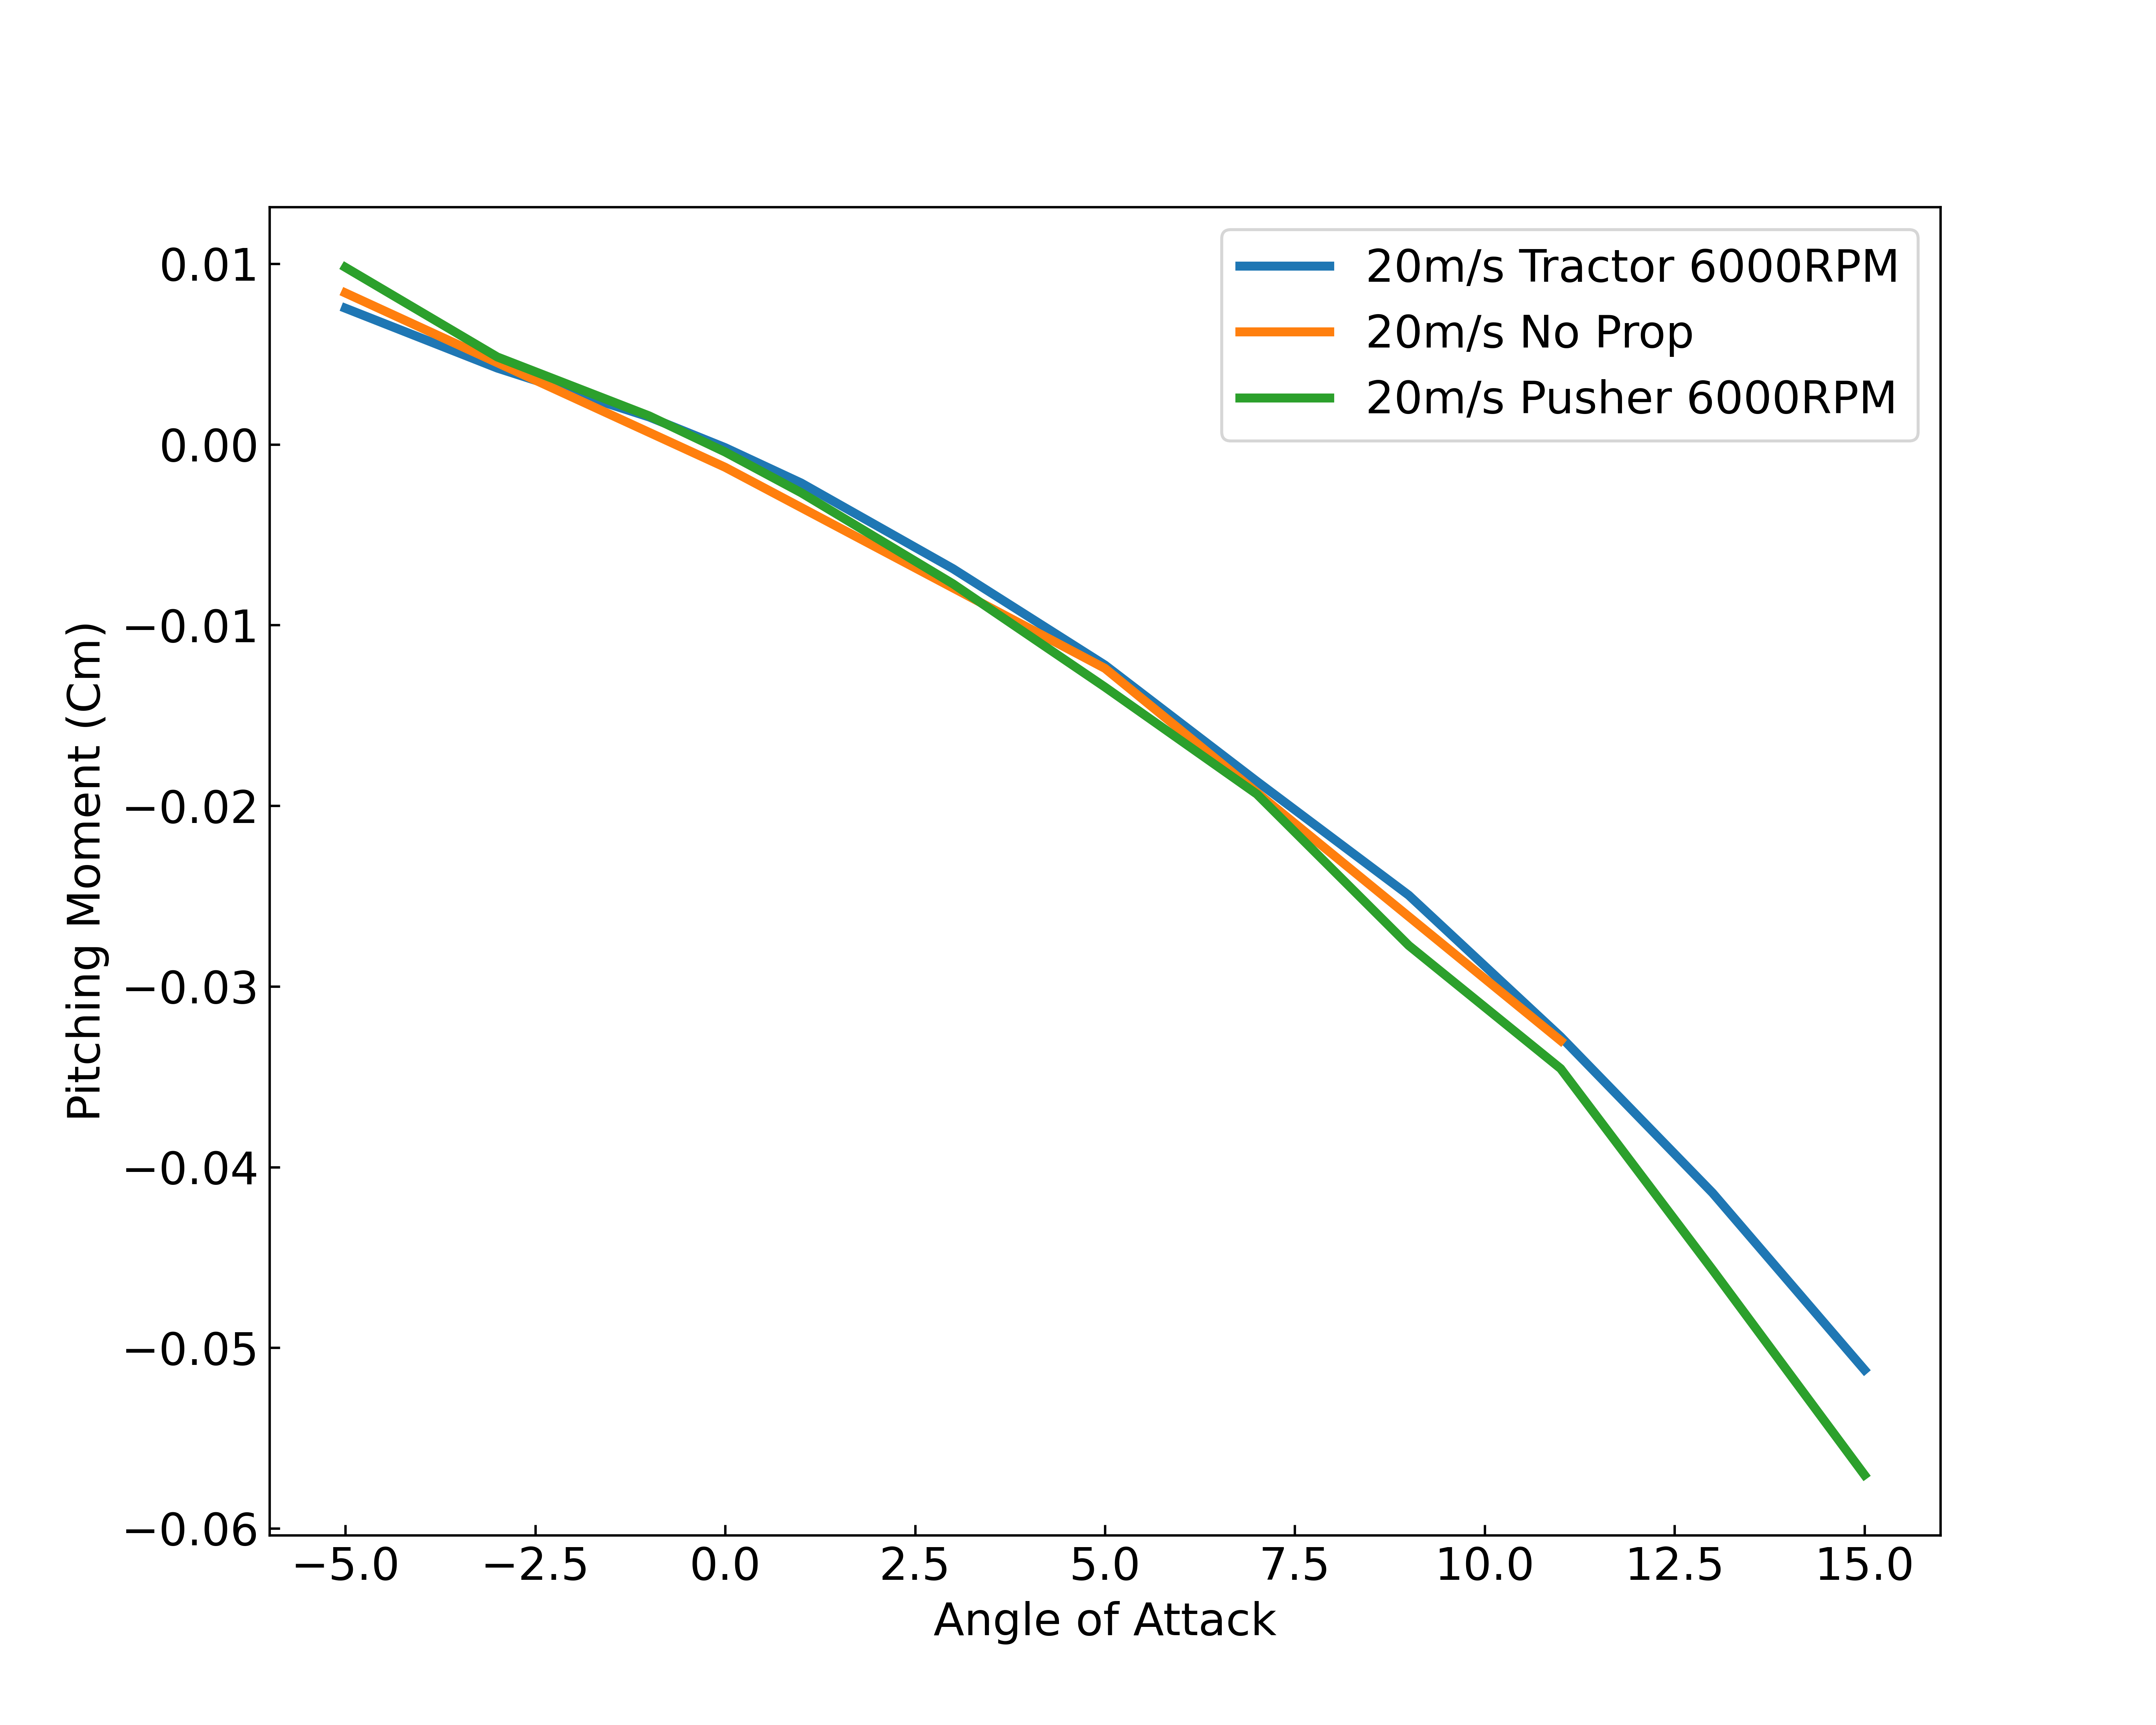
\includegraphics[width=\textwidth]{05_Results/Figs/Cm/20ms_6000RPM_Cm.png}
        \caption{Pitching Moment Coefficient at 20m/s airspeed and 6000RPM motor speed}
        \label{fig:Cm_20ms_6000}
    \end{subfigure}
    \begin{subfigure}[b]{0.467\textwidth}
        \centering
        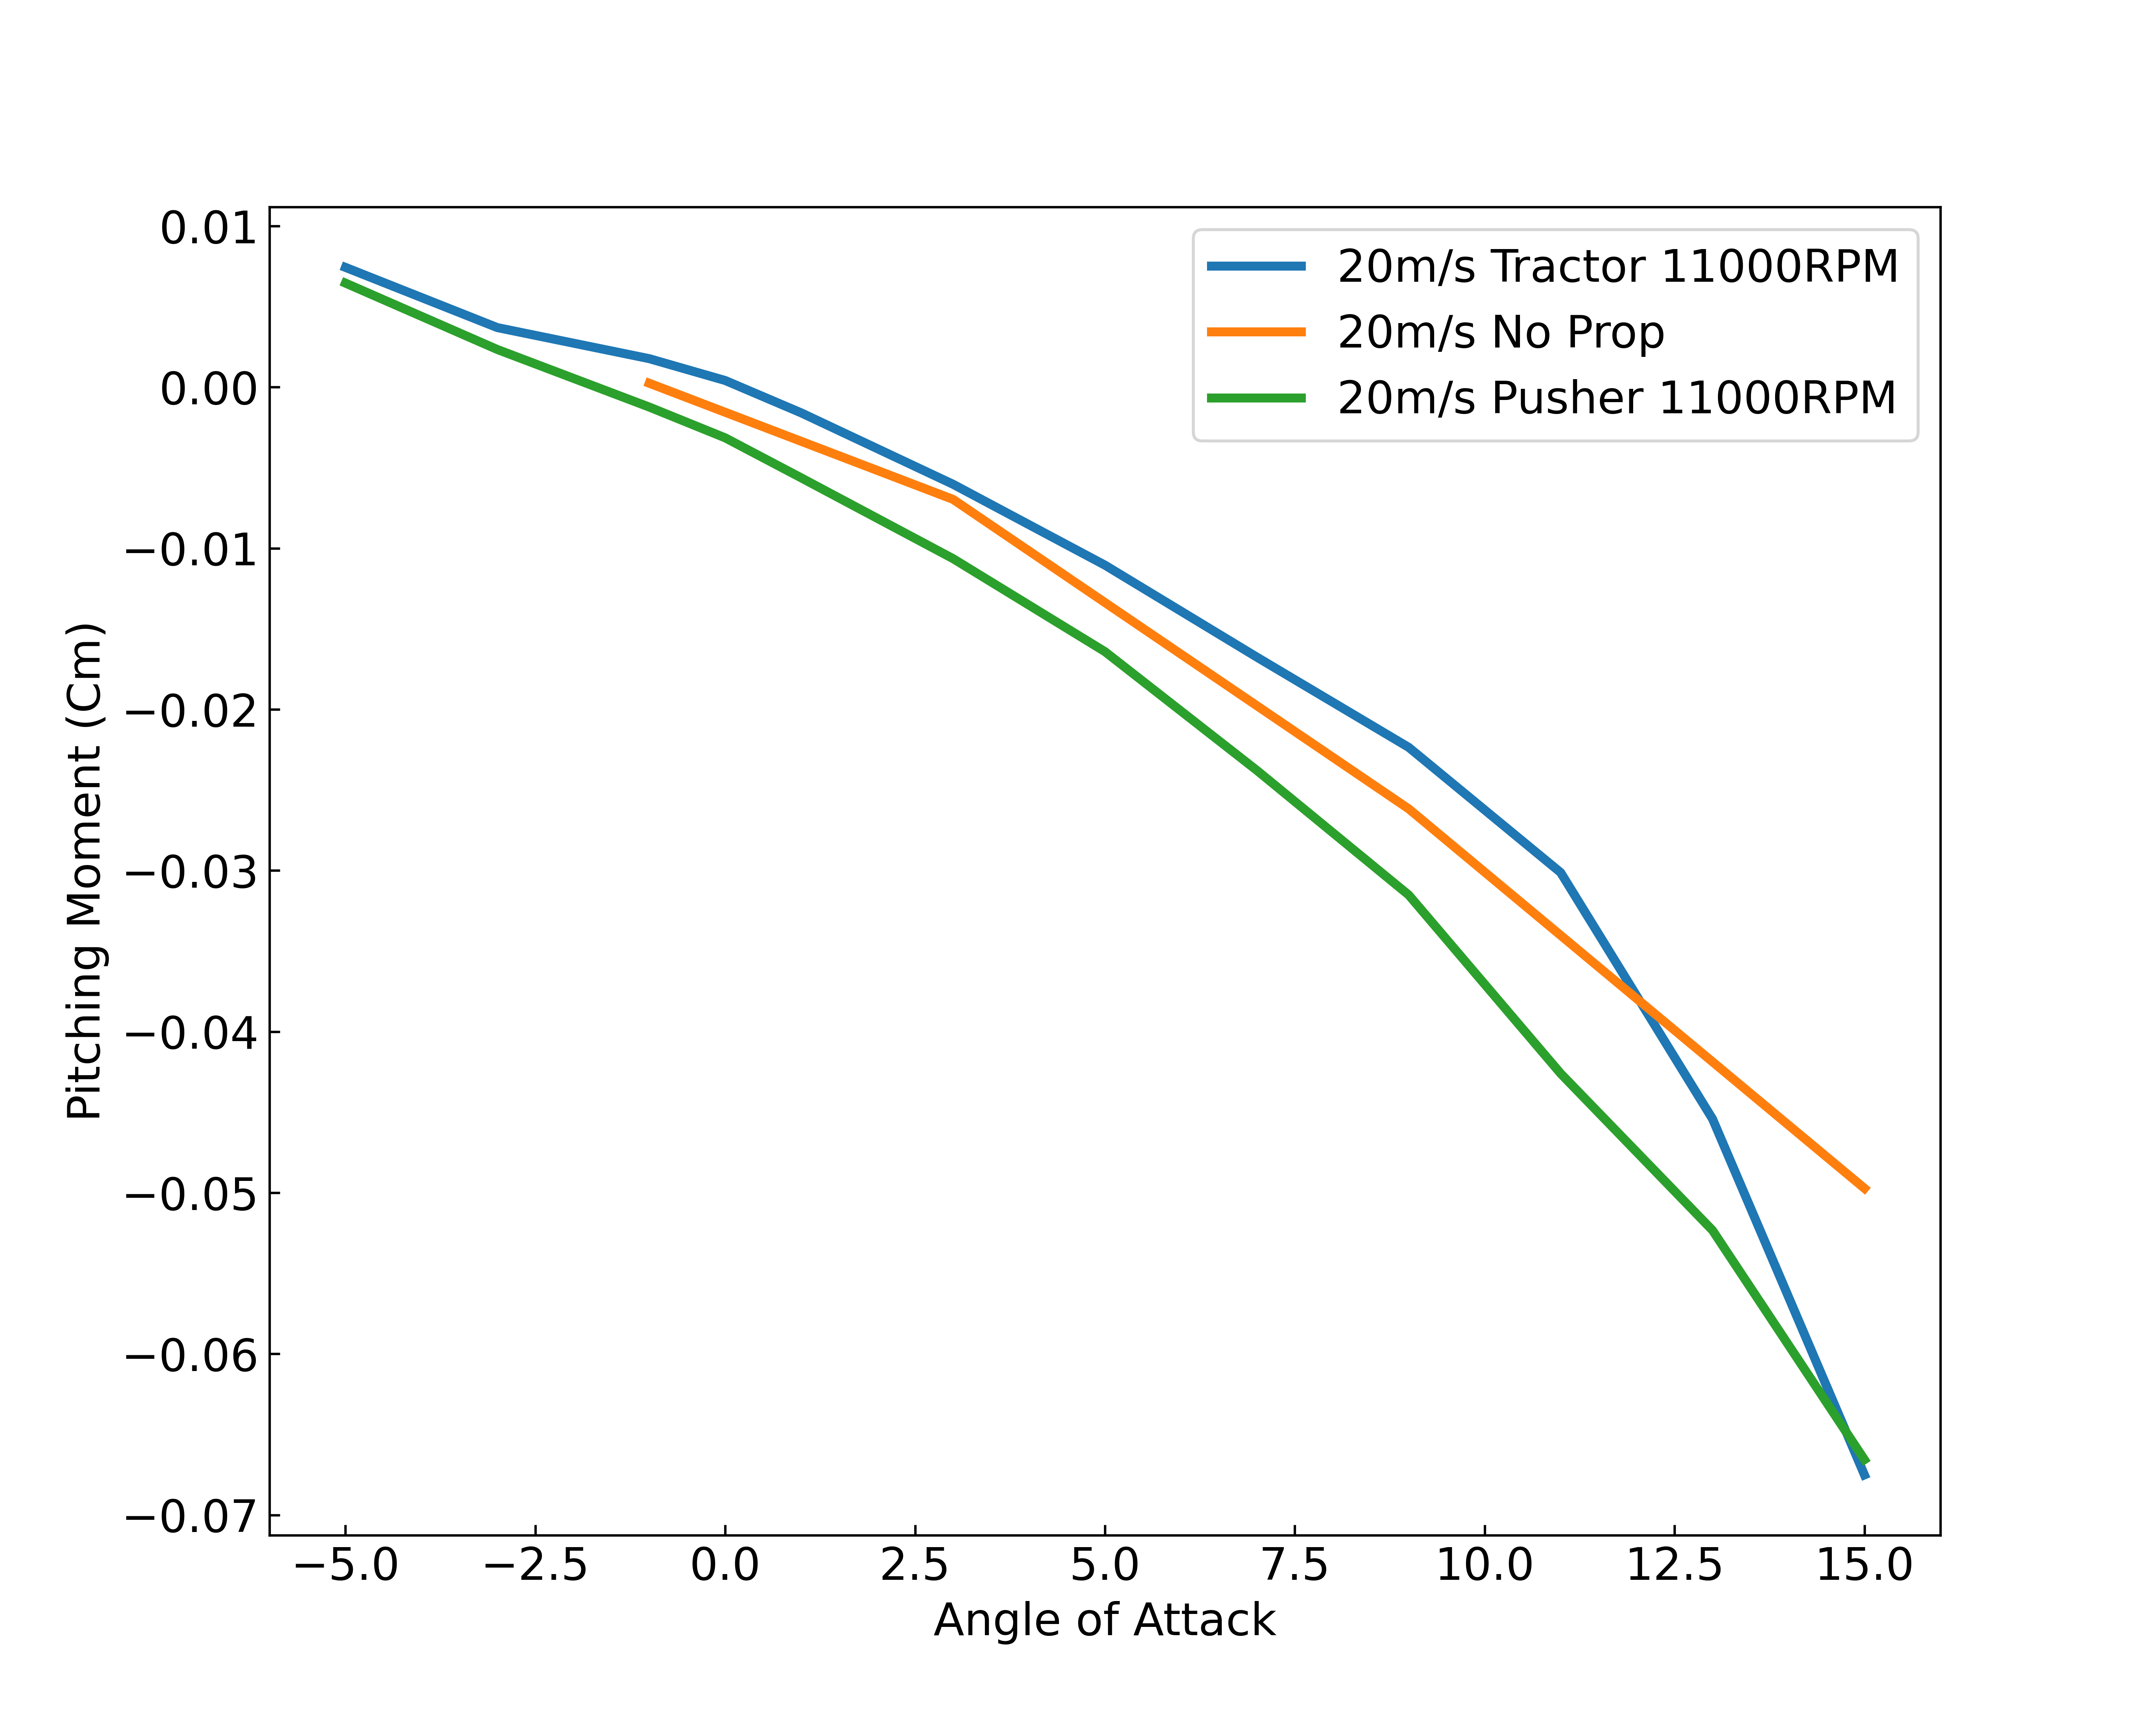
\includegraphics[width=\textwidth]{05_Results/Figs/Cm/20ms_11000RPM_Cm.png}
        \caption{Pitching Moment Coefficient at 20m/s airspeed and 11000RPM motor speed}
        \label{fig:Cm_20ms_11000}
    \end{subfigure}
    \label{fig:Cm_graphs}
\end{figure}



\subsection{Yawing Moment Coefficient}
The yawing coefficient was larger for the tractor configuration due to a larger moment arm 

\begin{figure}[H]
    \centering
    \begin{subfigure}[b]{0.467\textwidth}
        \centering
        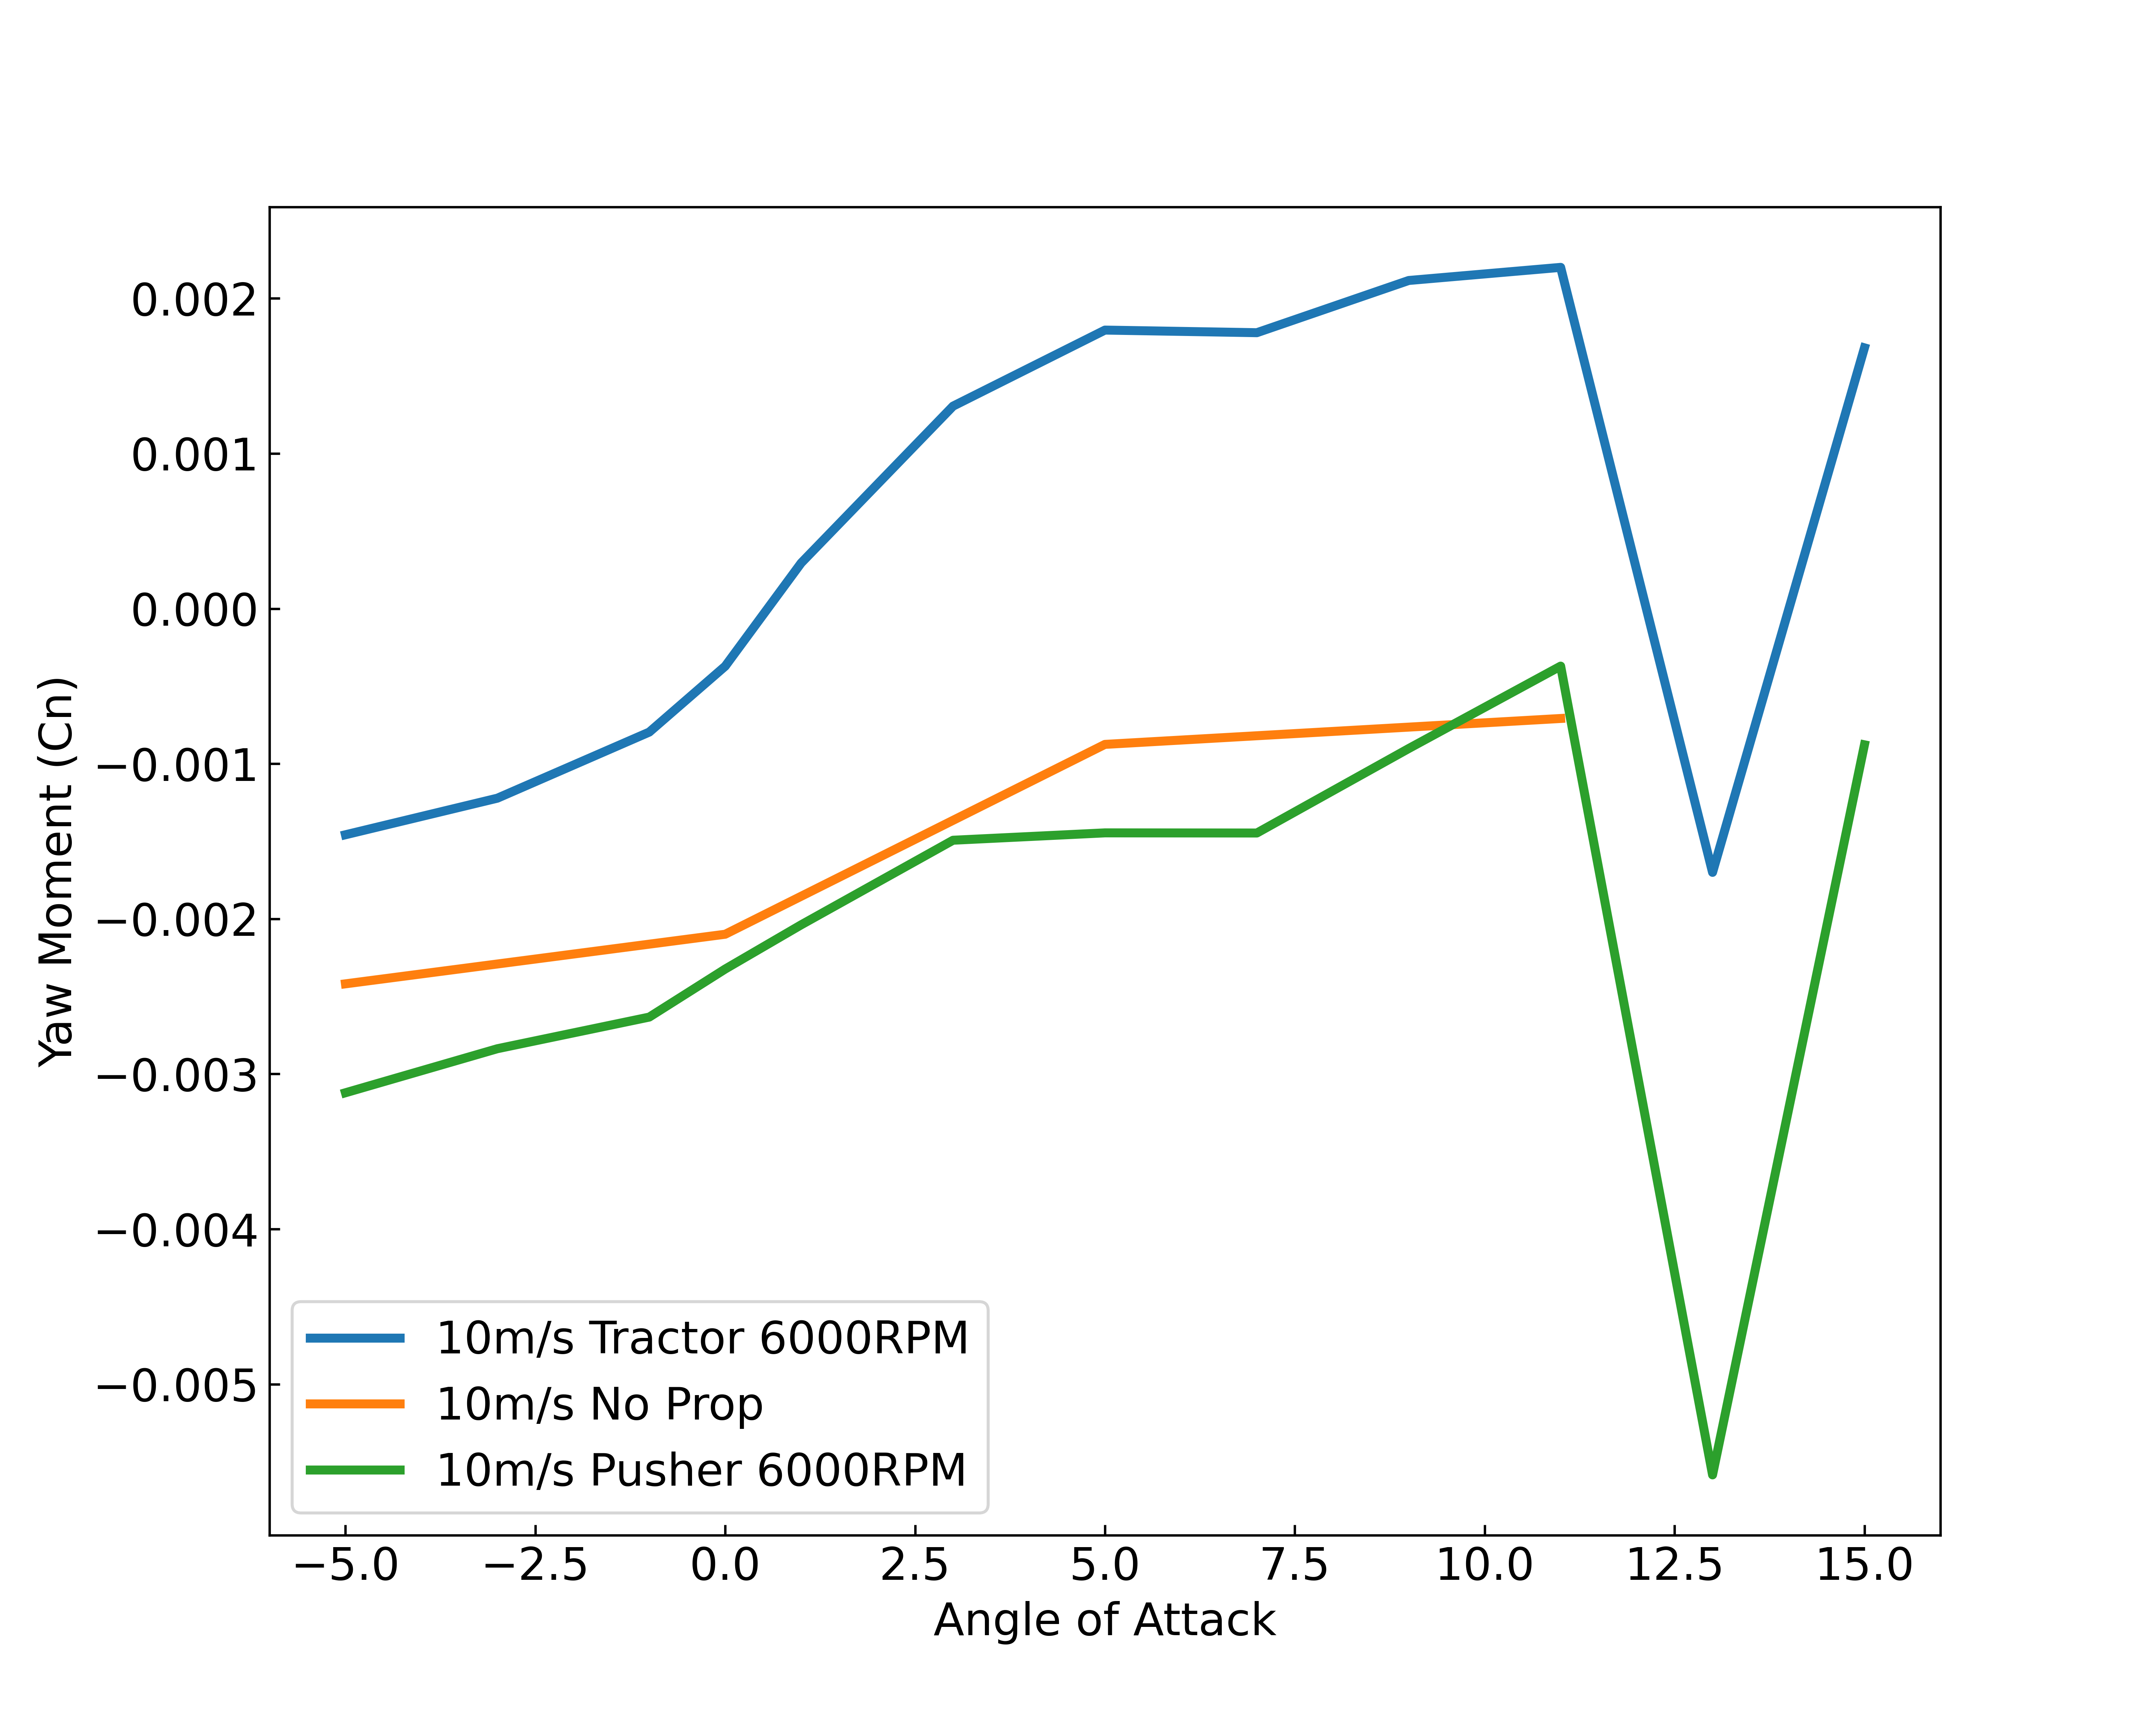
\includegraphics[width=\textwidth]{05_Results/Figs/Cn/10ms_6000RPM_Cn.png}
        \caption{Yawing Moment Coefficient at 10m/s airspeed and 6000RPM motor speed}
        \label{fig:Cn_10ms_6000}
    \end{subfigure}
    \begin{subfigure}[b]{0.467\textwidth}
        \centering
        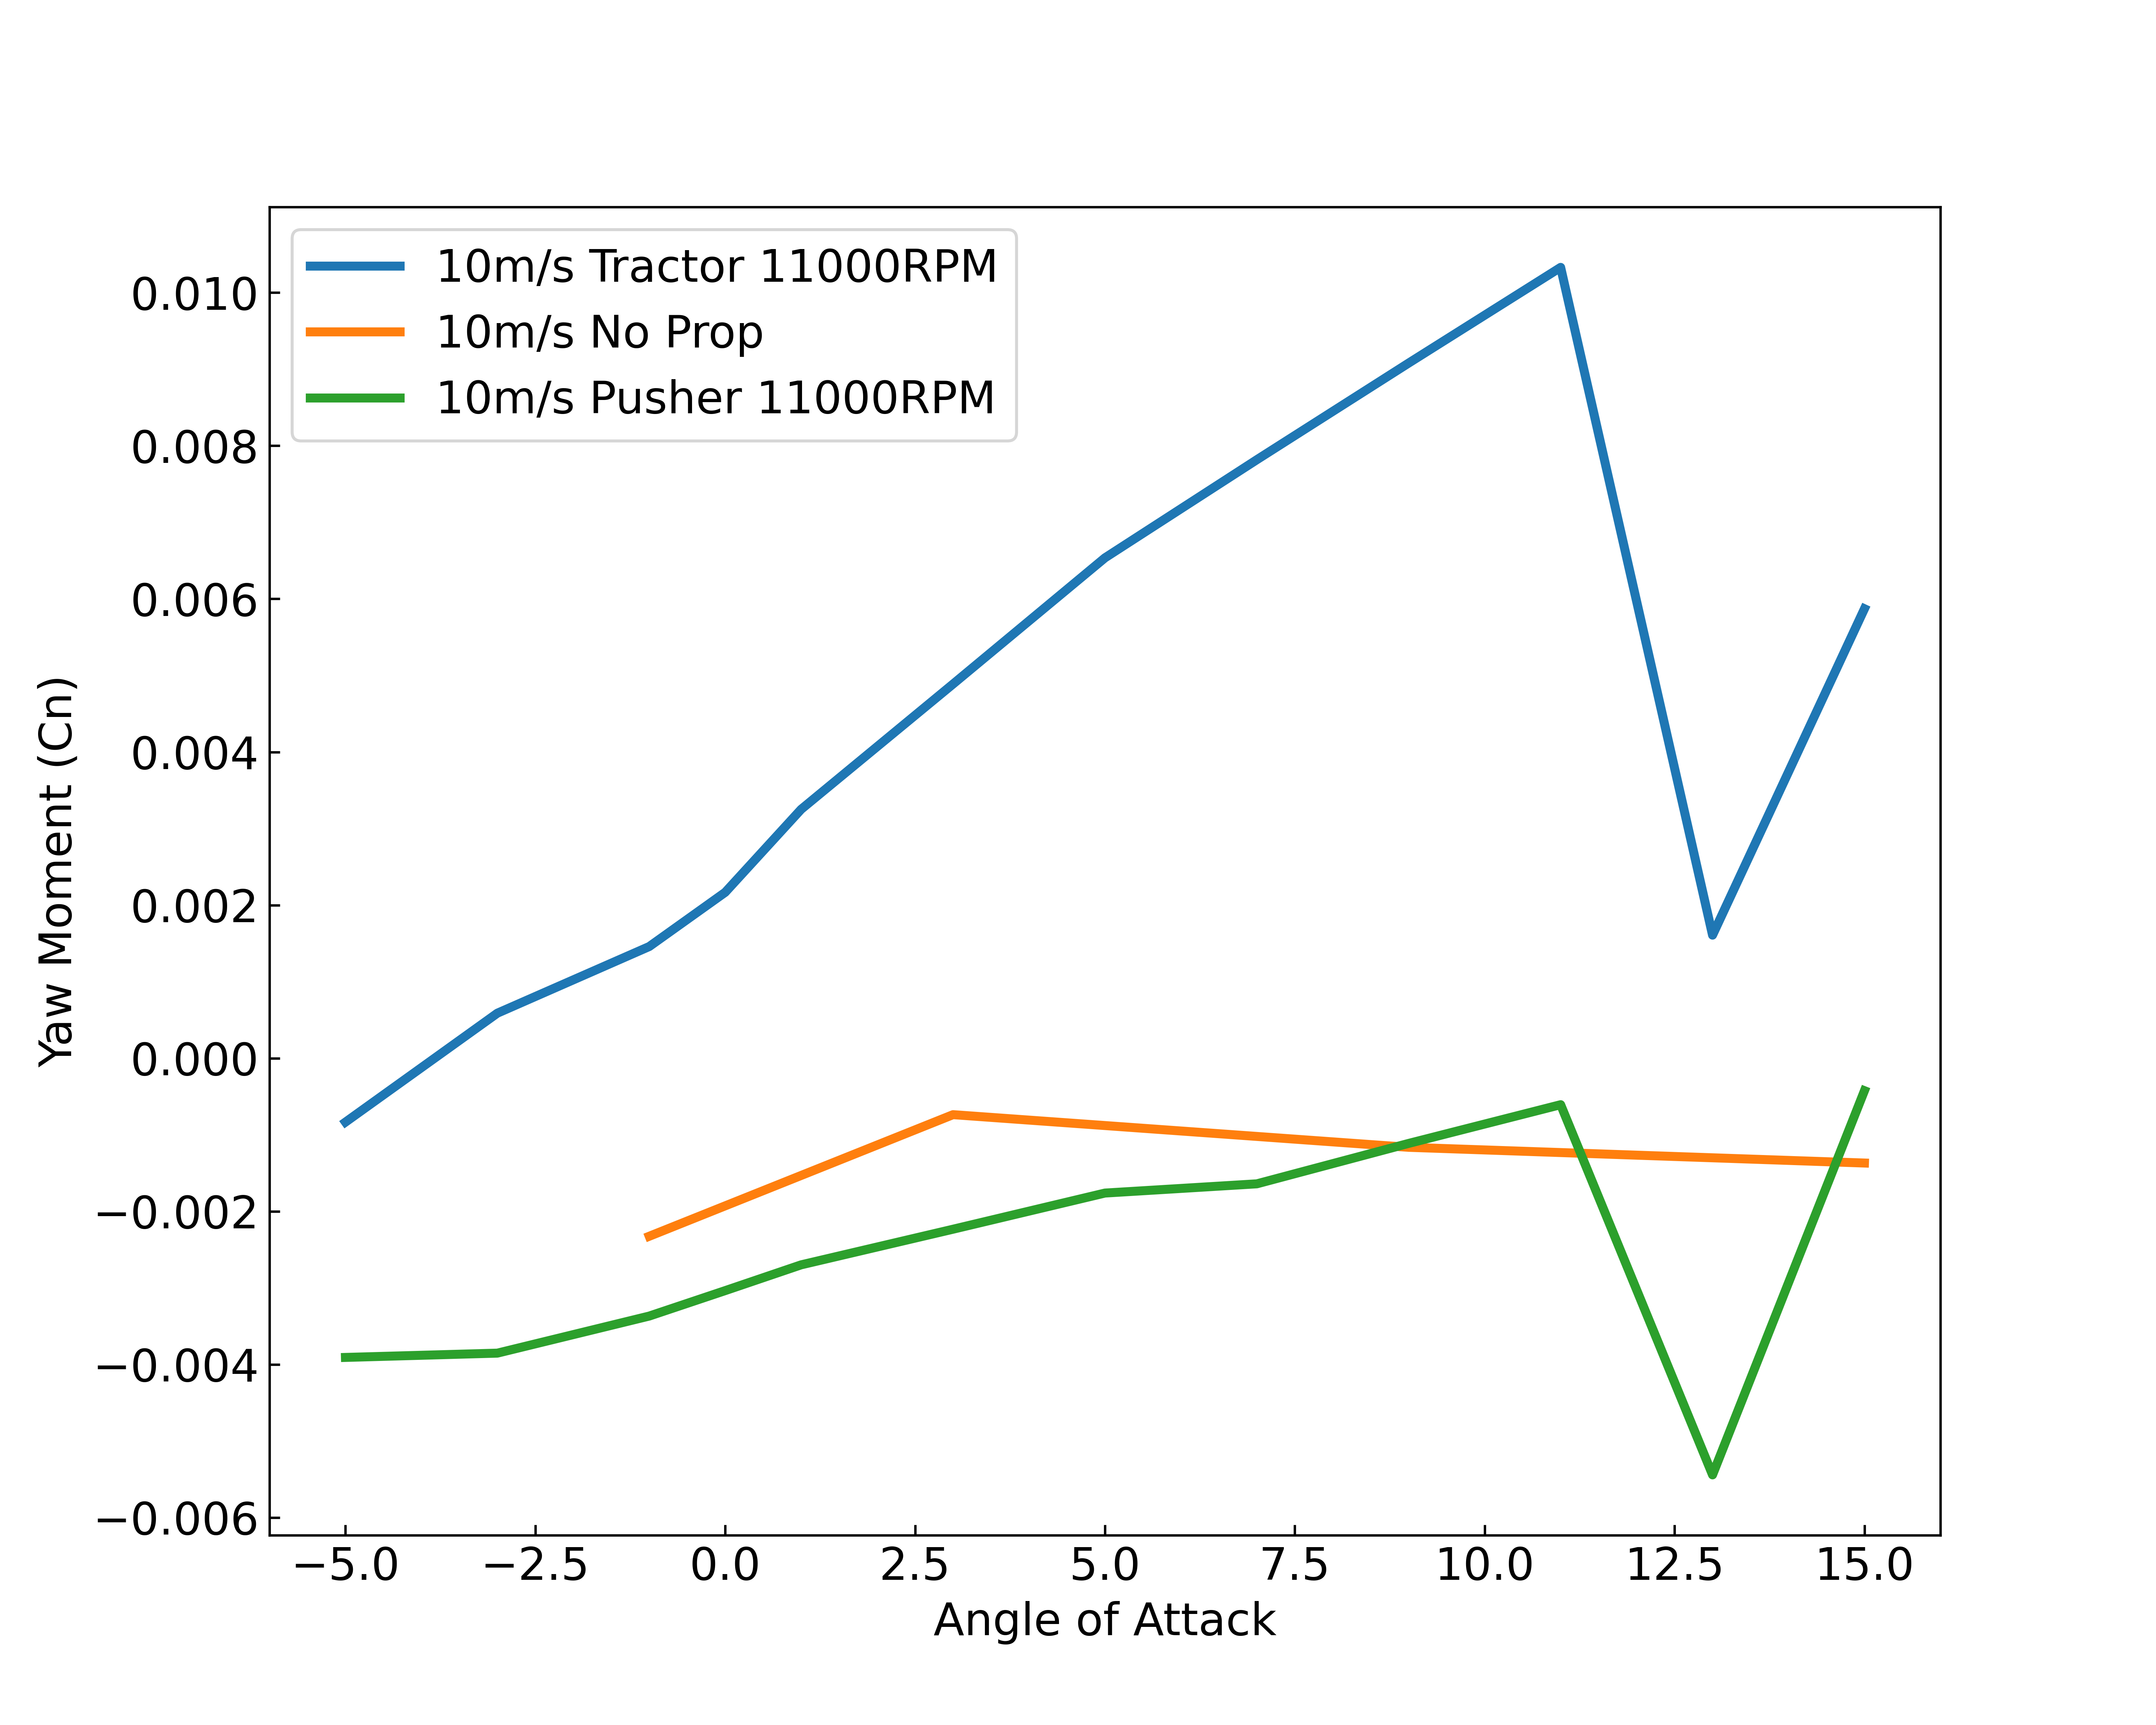
\includegraphics[width=\textwidth]{05_Results/Figs/Cn/10ms_11000RPM_Cn.png}
        \caption{Yawing Moment Coefficient at 10m/s airspeed and 11000RPM motor speed}
        \label{fig:Cn_10ms_11000}
    \end{subfigure}
    \begin{subfigure}[b]{0.467\textwidth}
        \centering
        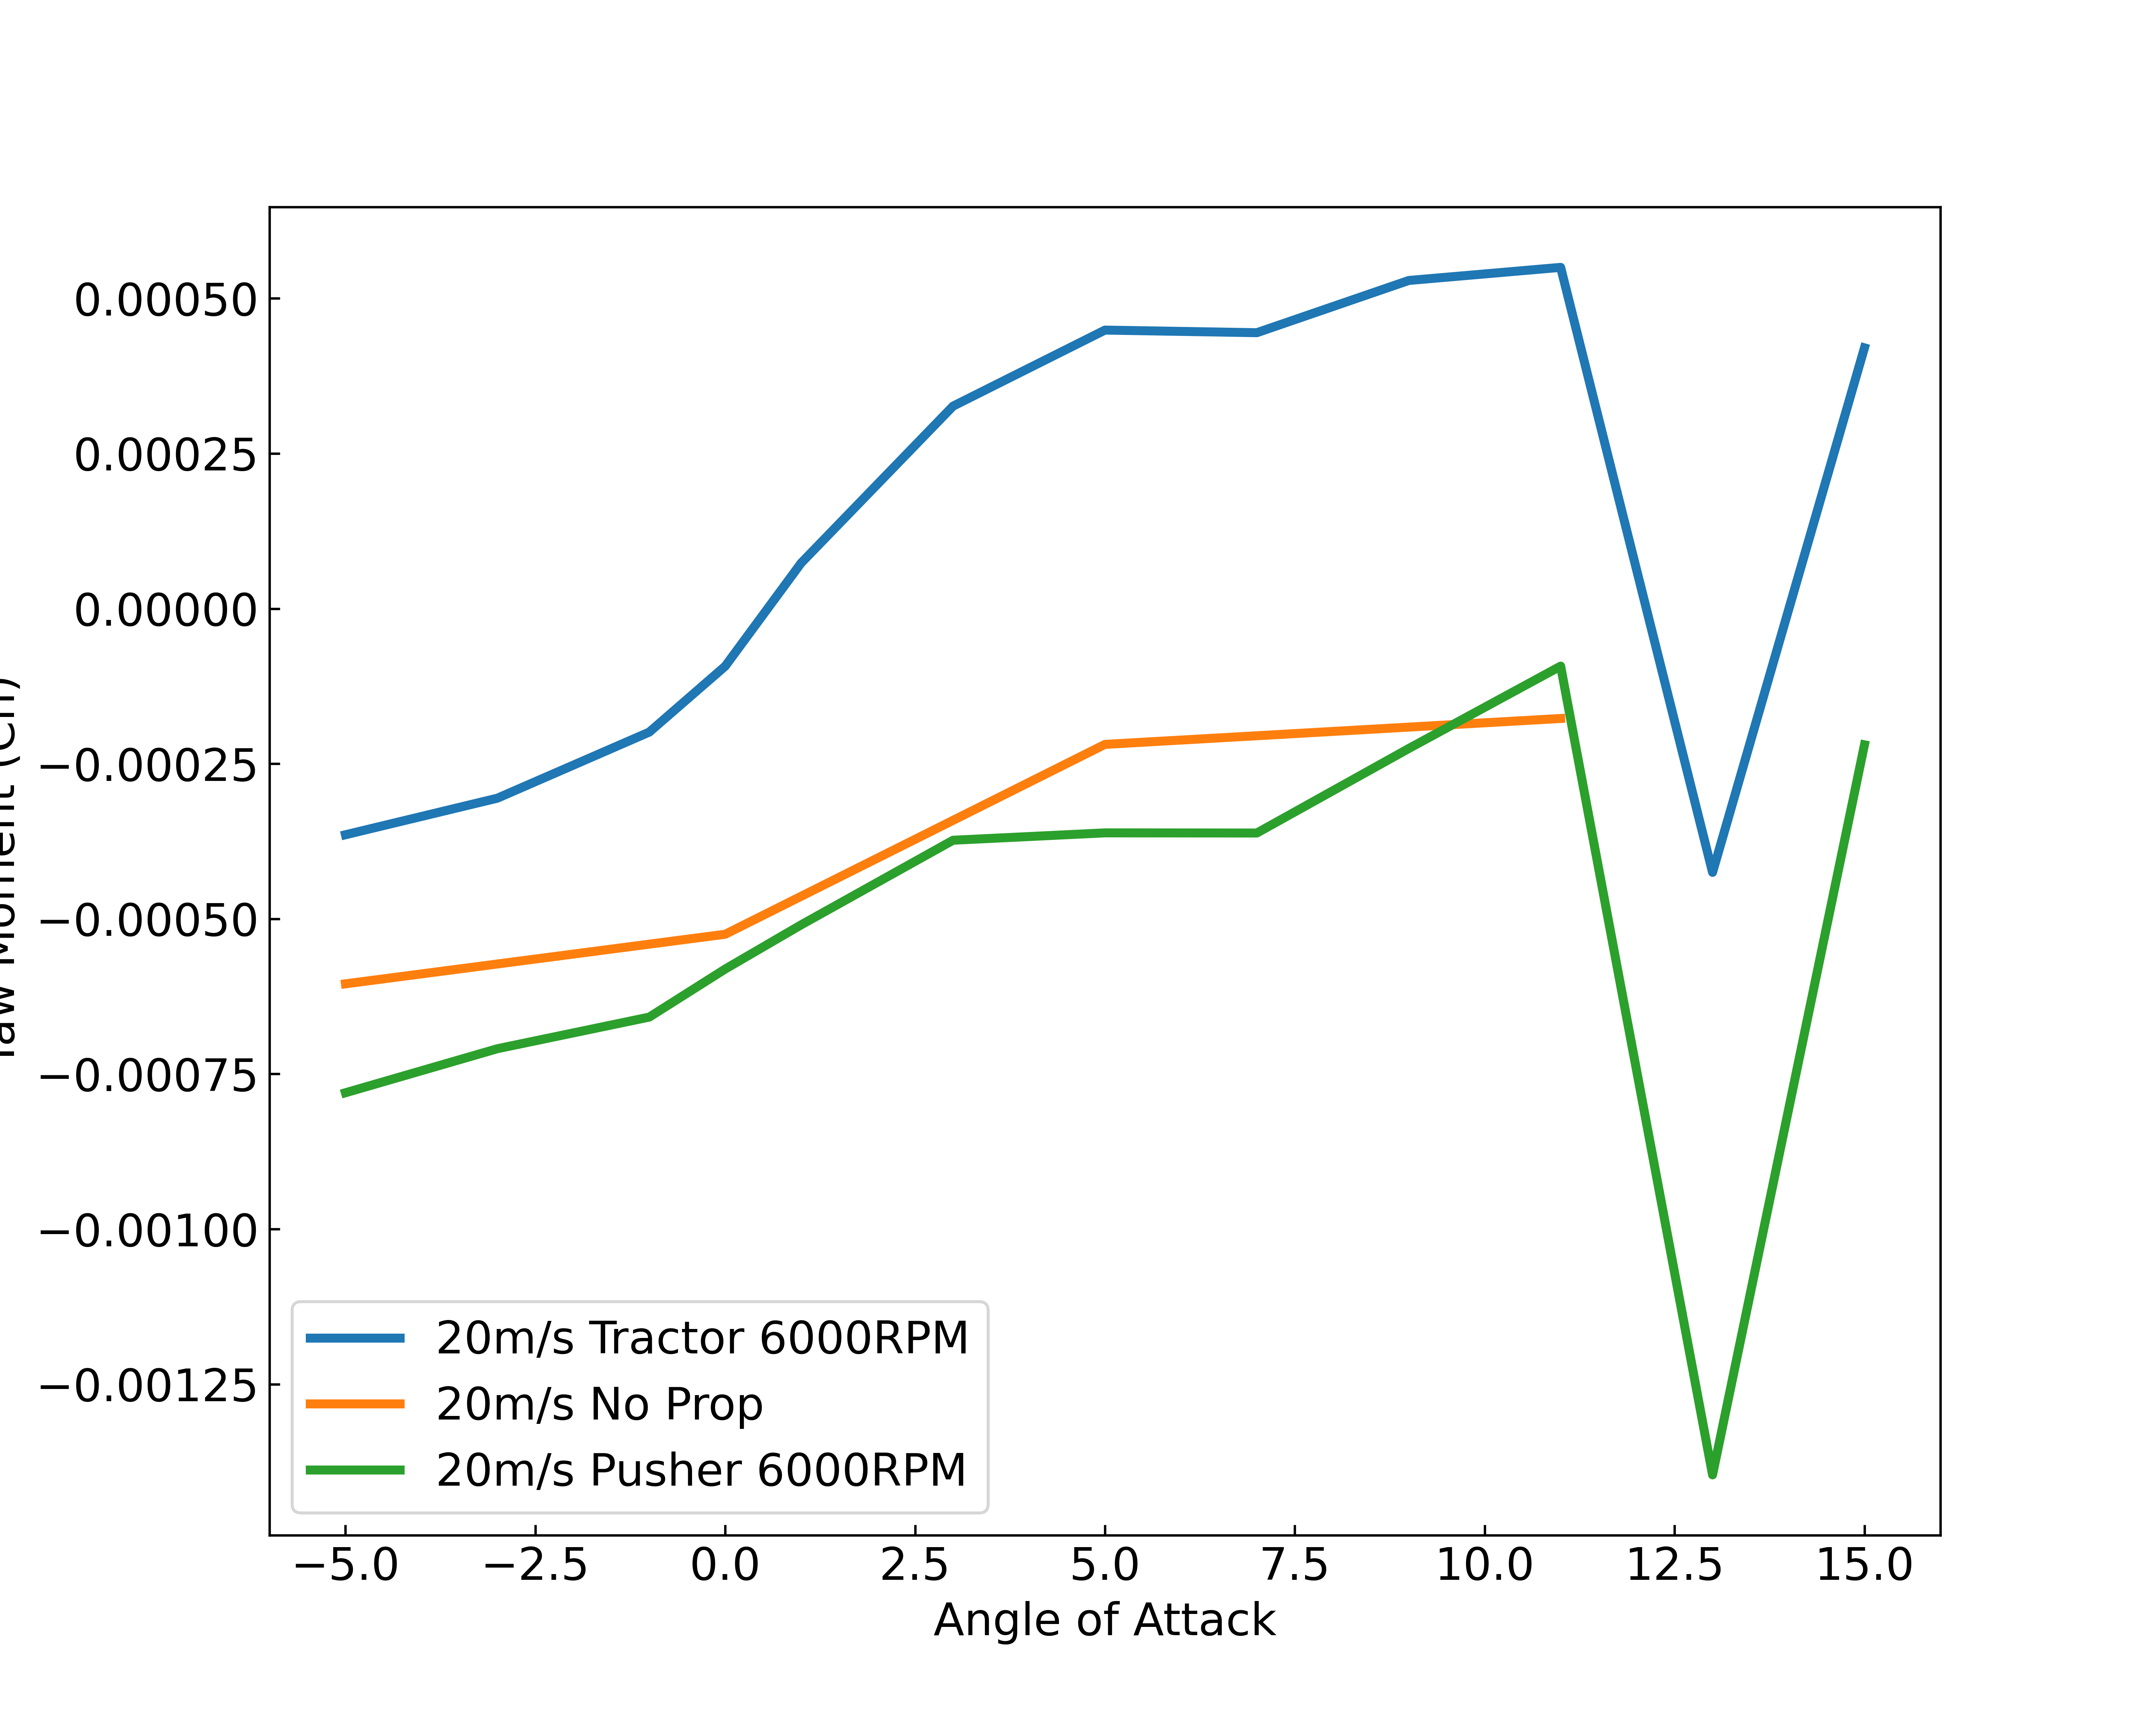
\includegraphics[width=\textwidth]{05_Results/Figs/Cn/20ms_6000RPM_Cn.png}
        \caption{Yawing Moment Coefficient at 20m/s airspeed and 6000RPM motor speed}
        \label{fig:Cn_20ms_6000}
    \end{subfigure}
    \begin{subfigure}[b]{0.467\textwidth}
        \centering
        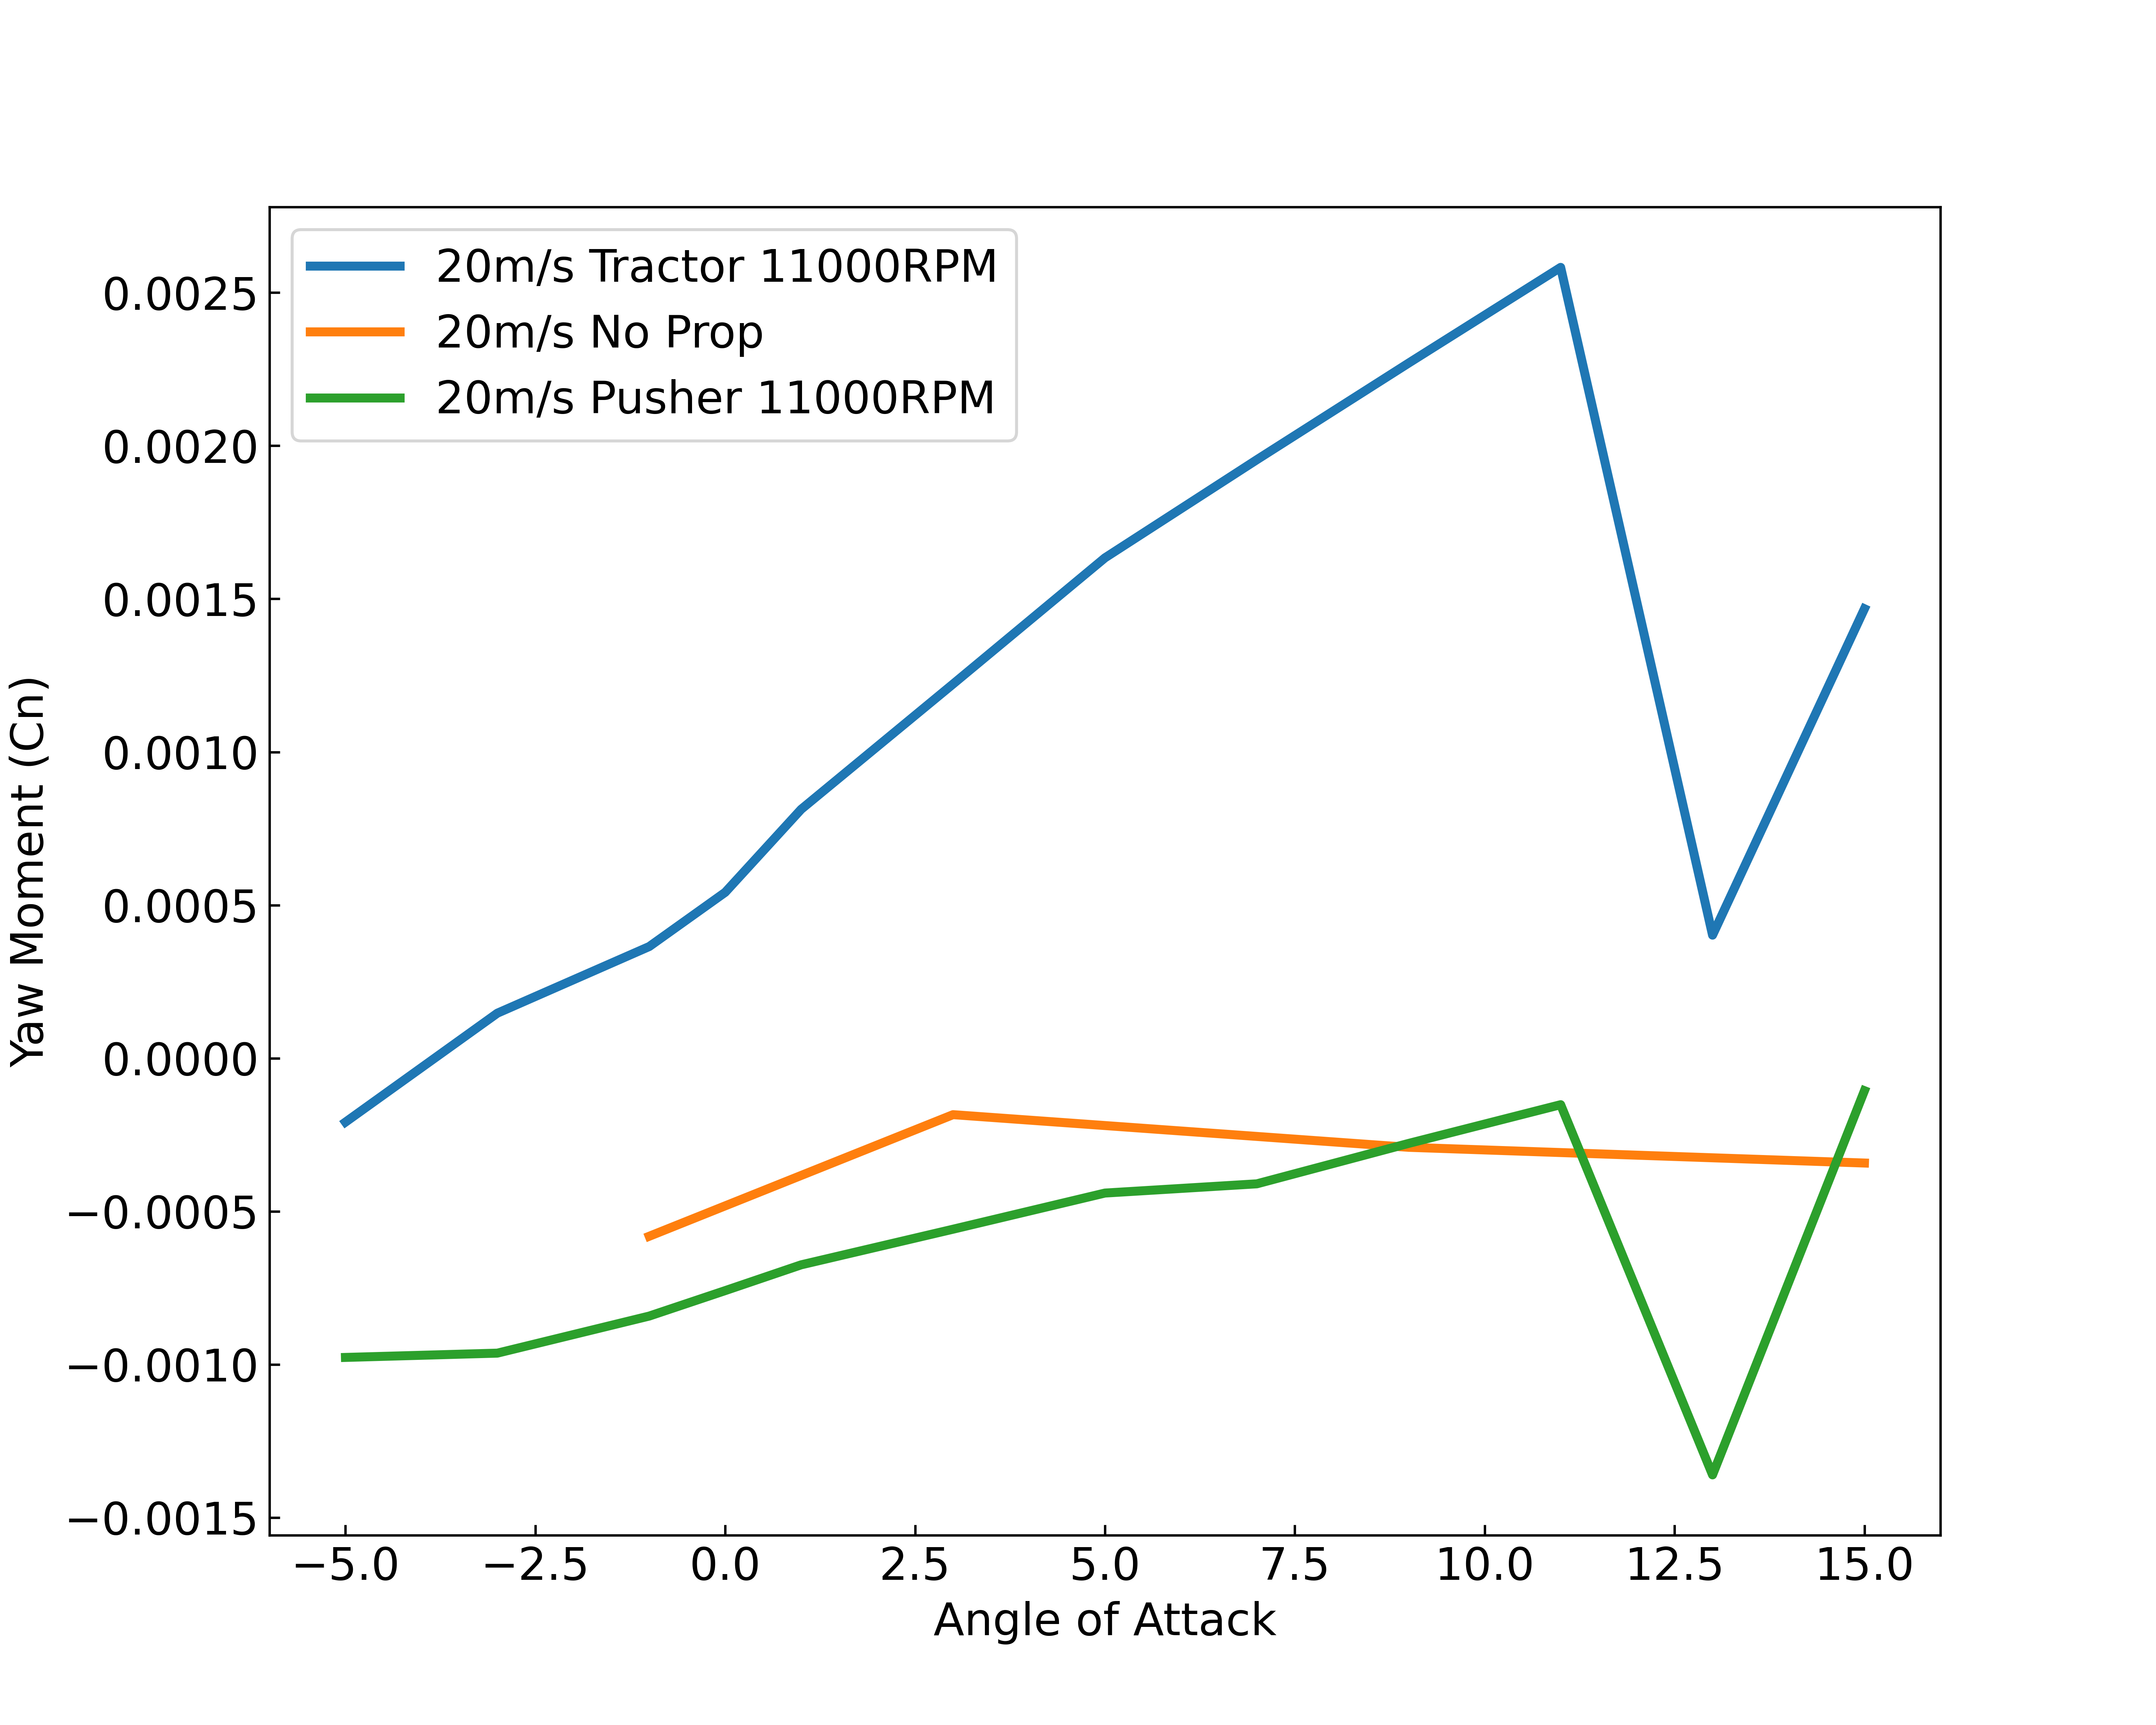
\includegraphics[width=\textwidth]{05_Results/Figs/Cn/20ms_11000RPM_Cn.png}
        \caption{Yawing Moment Coefficient at 20m/s airspeed and 11000RPM motor speed}
        \label{fig:Cn_20ms_11000}
    \end{subfigure}
\end{figure}


\subsection{Rolling Moment Coefficient}

\begin{figure}[H]
    \centering
    \begin{subfigure}[b]{0.467\textwidth}
        \centering
        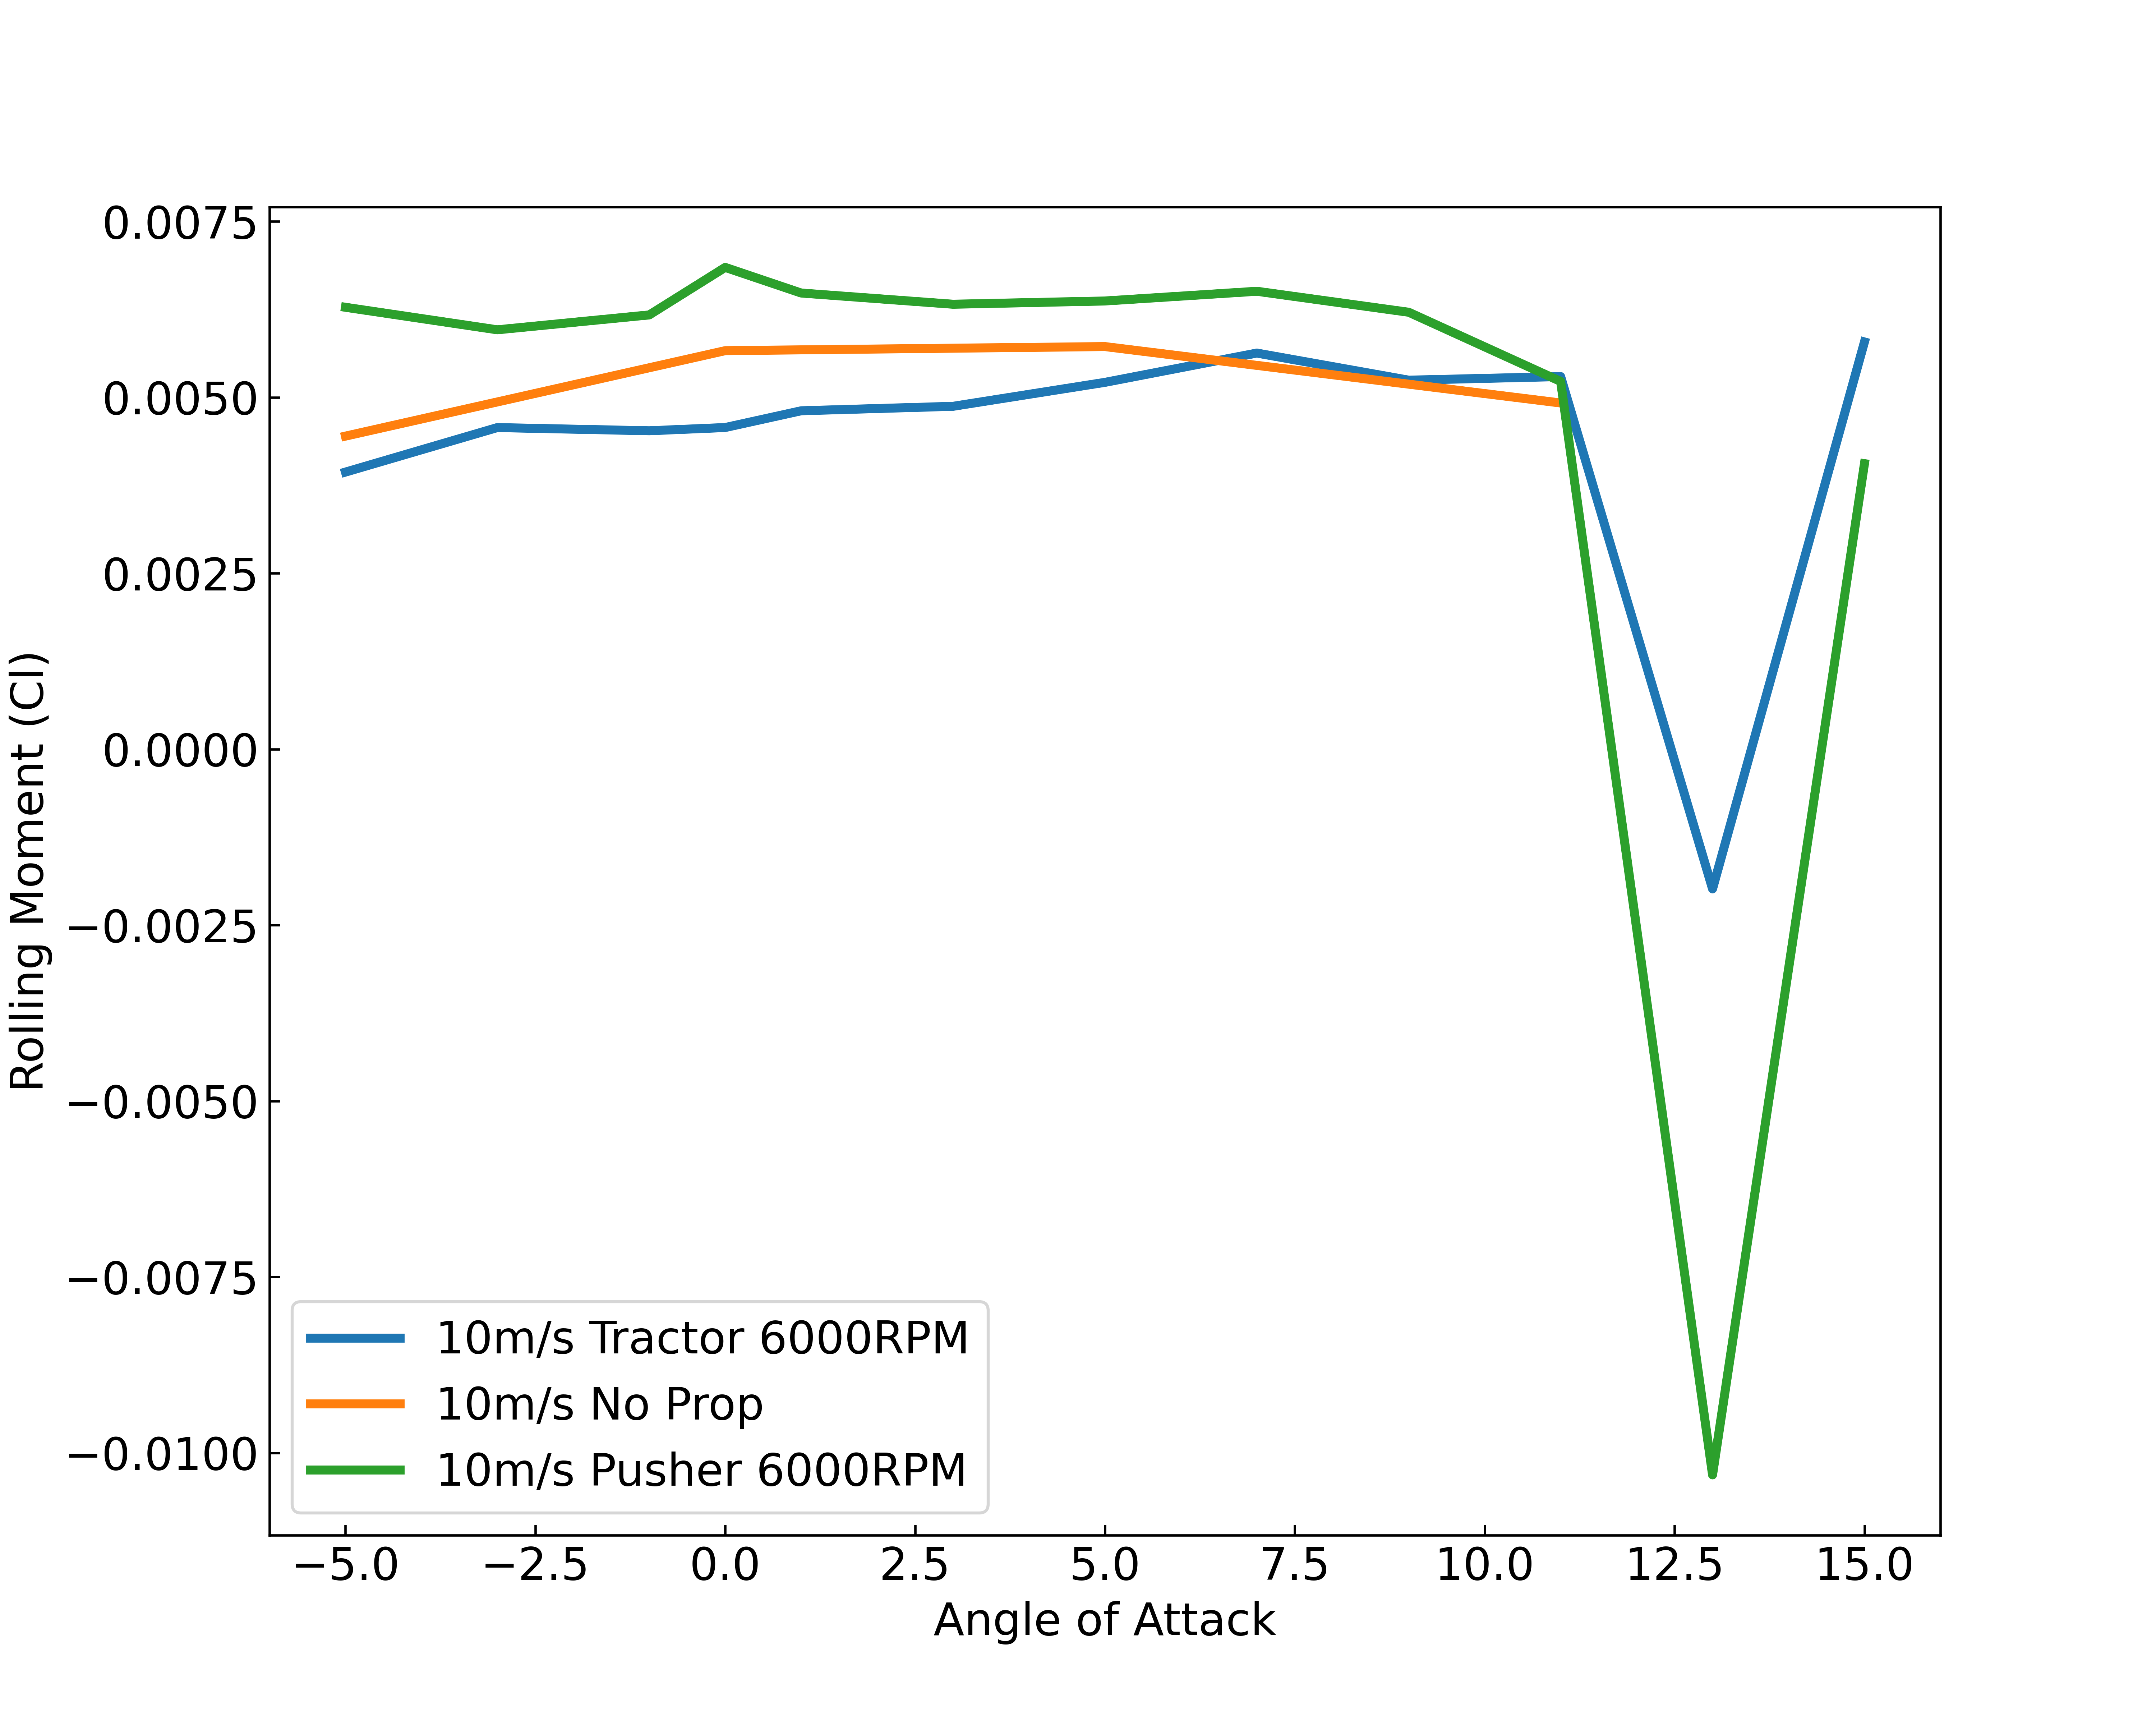
\includegraphics[width=\textwidth]{05_Results/Figs/Cl_roll/10ms_6000RPM_Cl_roll.png}
        \caption{Rolling Moment Coefficient at 10m/s airspeed and 6000RPM motor speed}
        \label{fig:Cl_roll_10ms_6000}
    \end{subfigure}
    \begin{subfigure}[b]{0.467\textwidth}
        \centering
        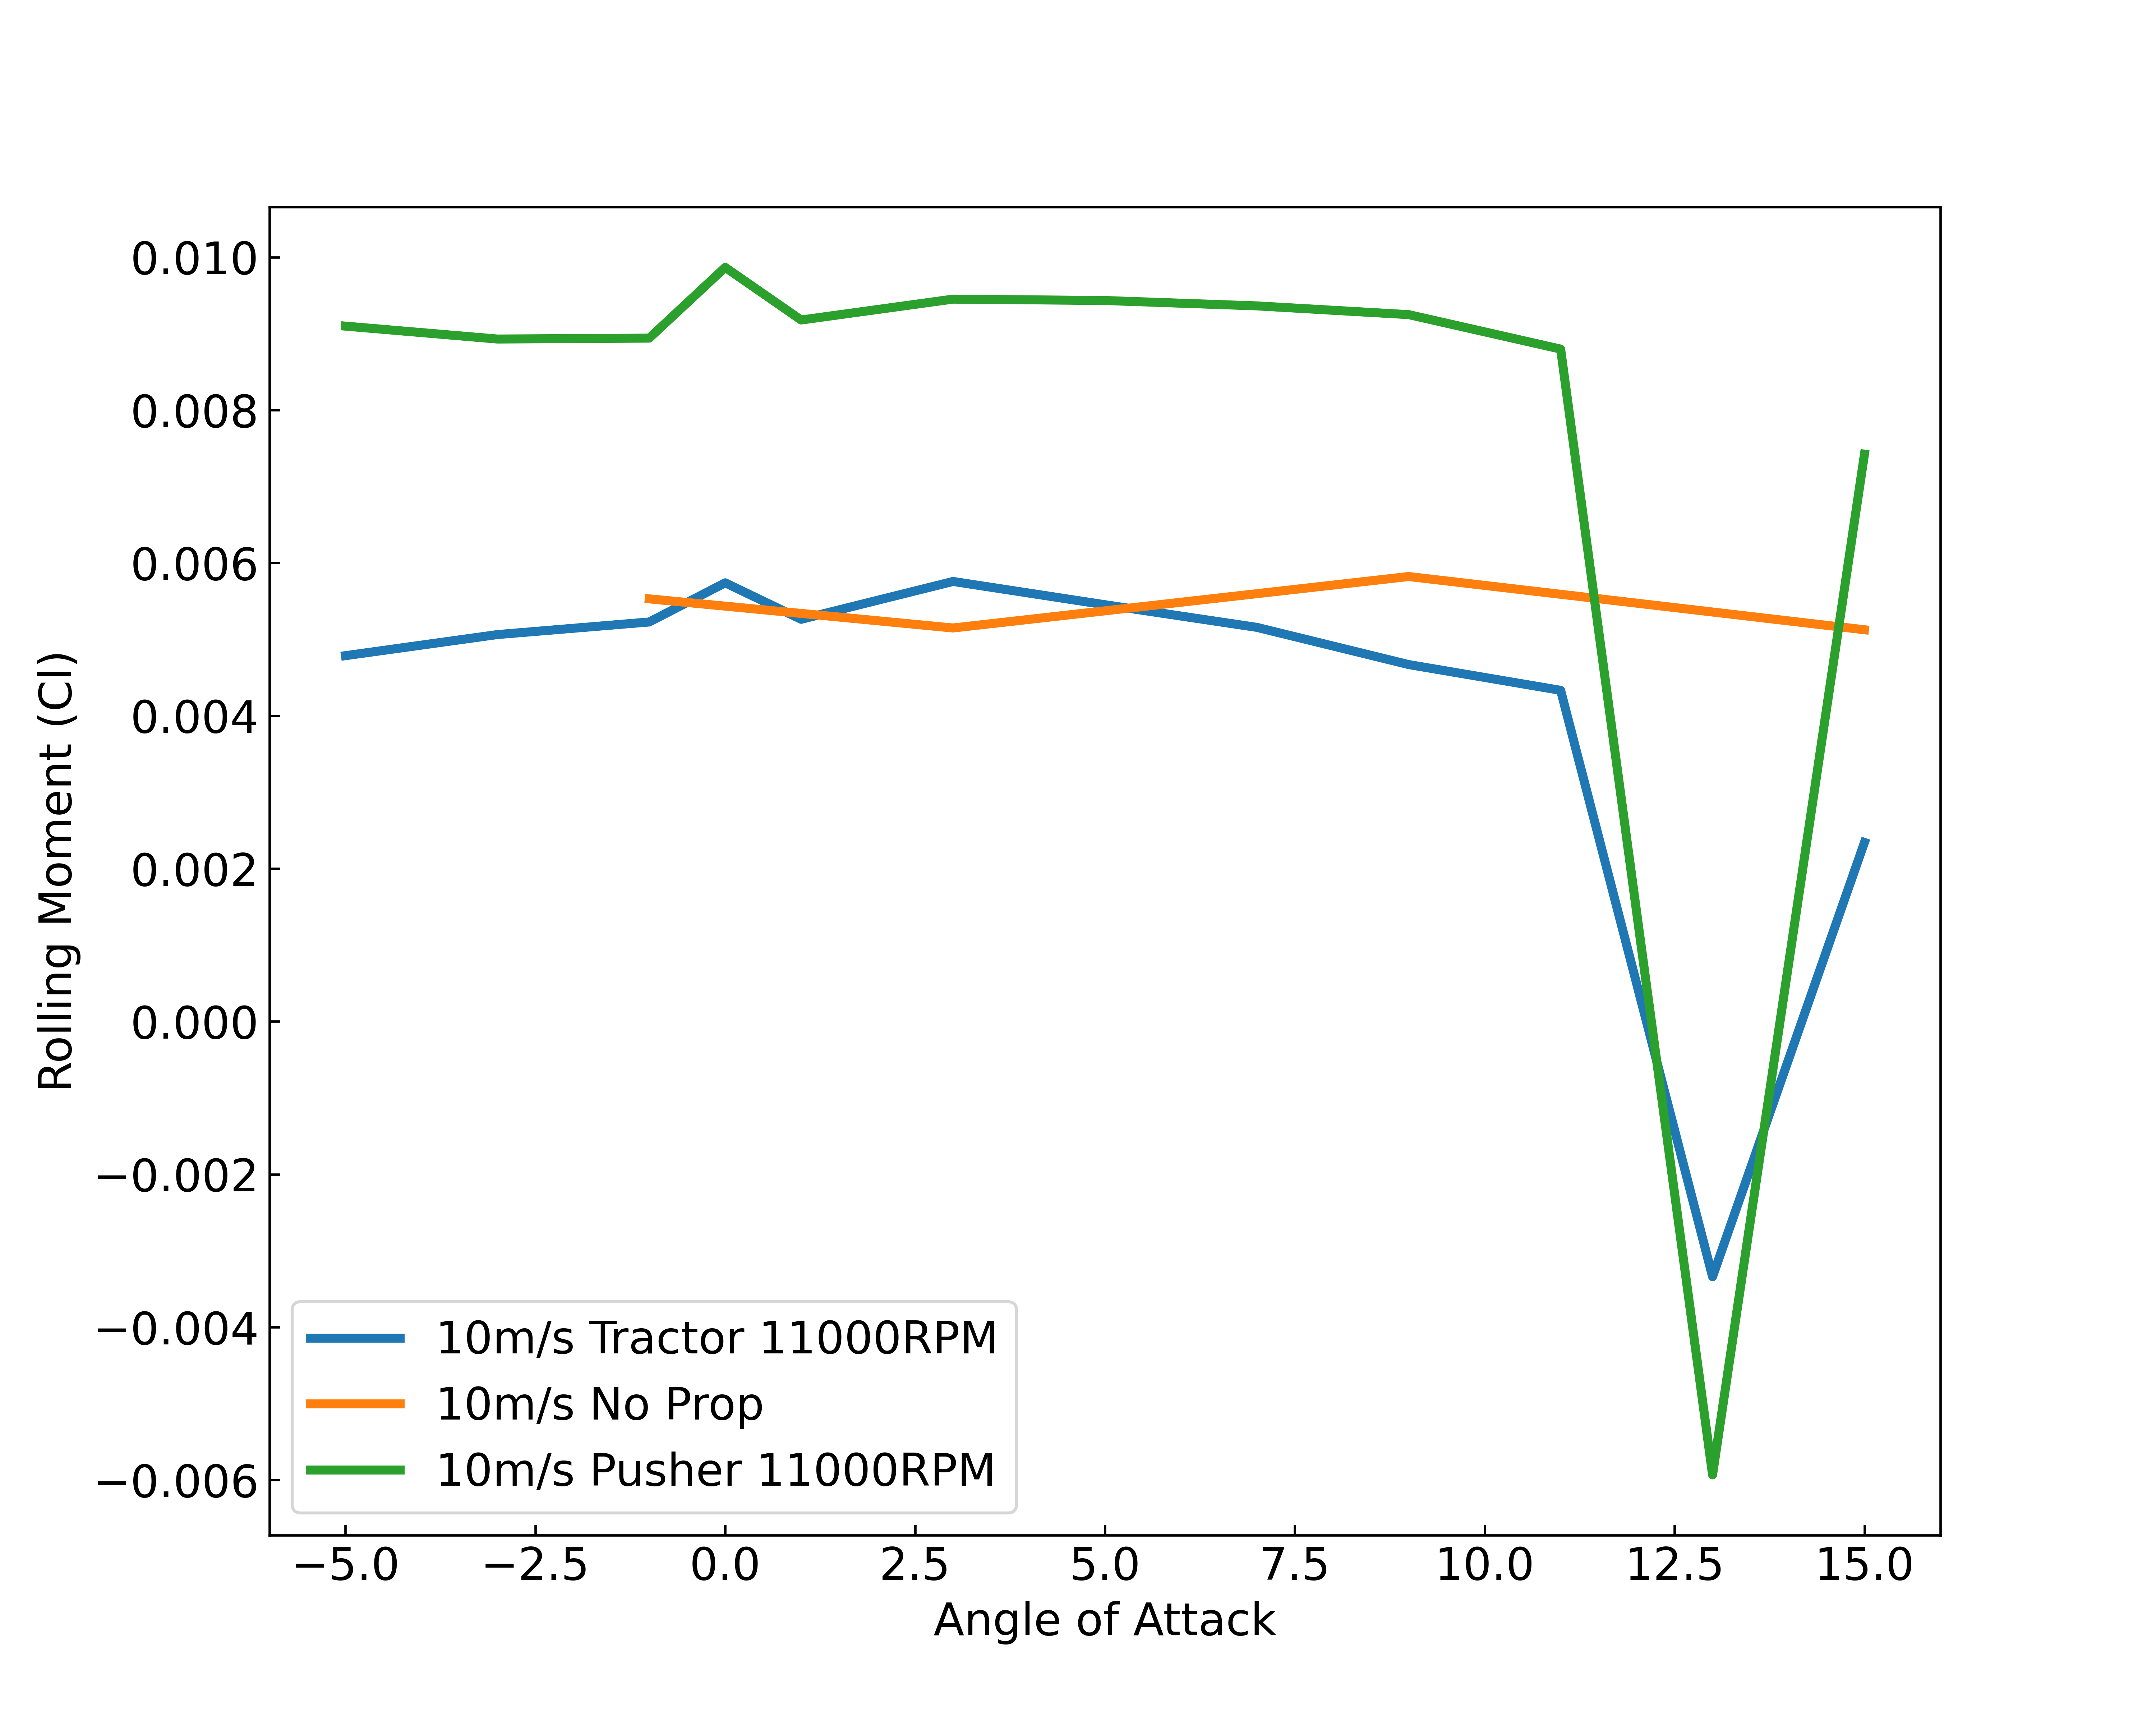
\includegraphics[width=\textwidth]{05_Results/Figs/Cl_roll/10ms_11000RPM_Cl.png}
        \caption{Rolling Moment Coefficient at 10m/s airspeed and 11000RPM motor speed}
        \label{fig:Cl_roll_10ms_11000}
    \end{subfigure}
    \begin{subfigure}[b]{0.467\textwidth}
        \centering
        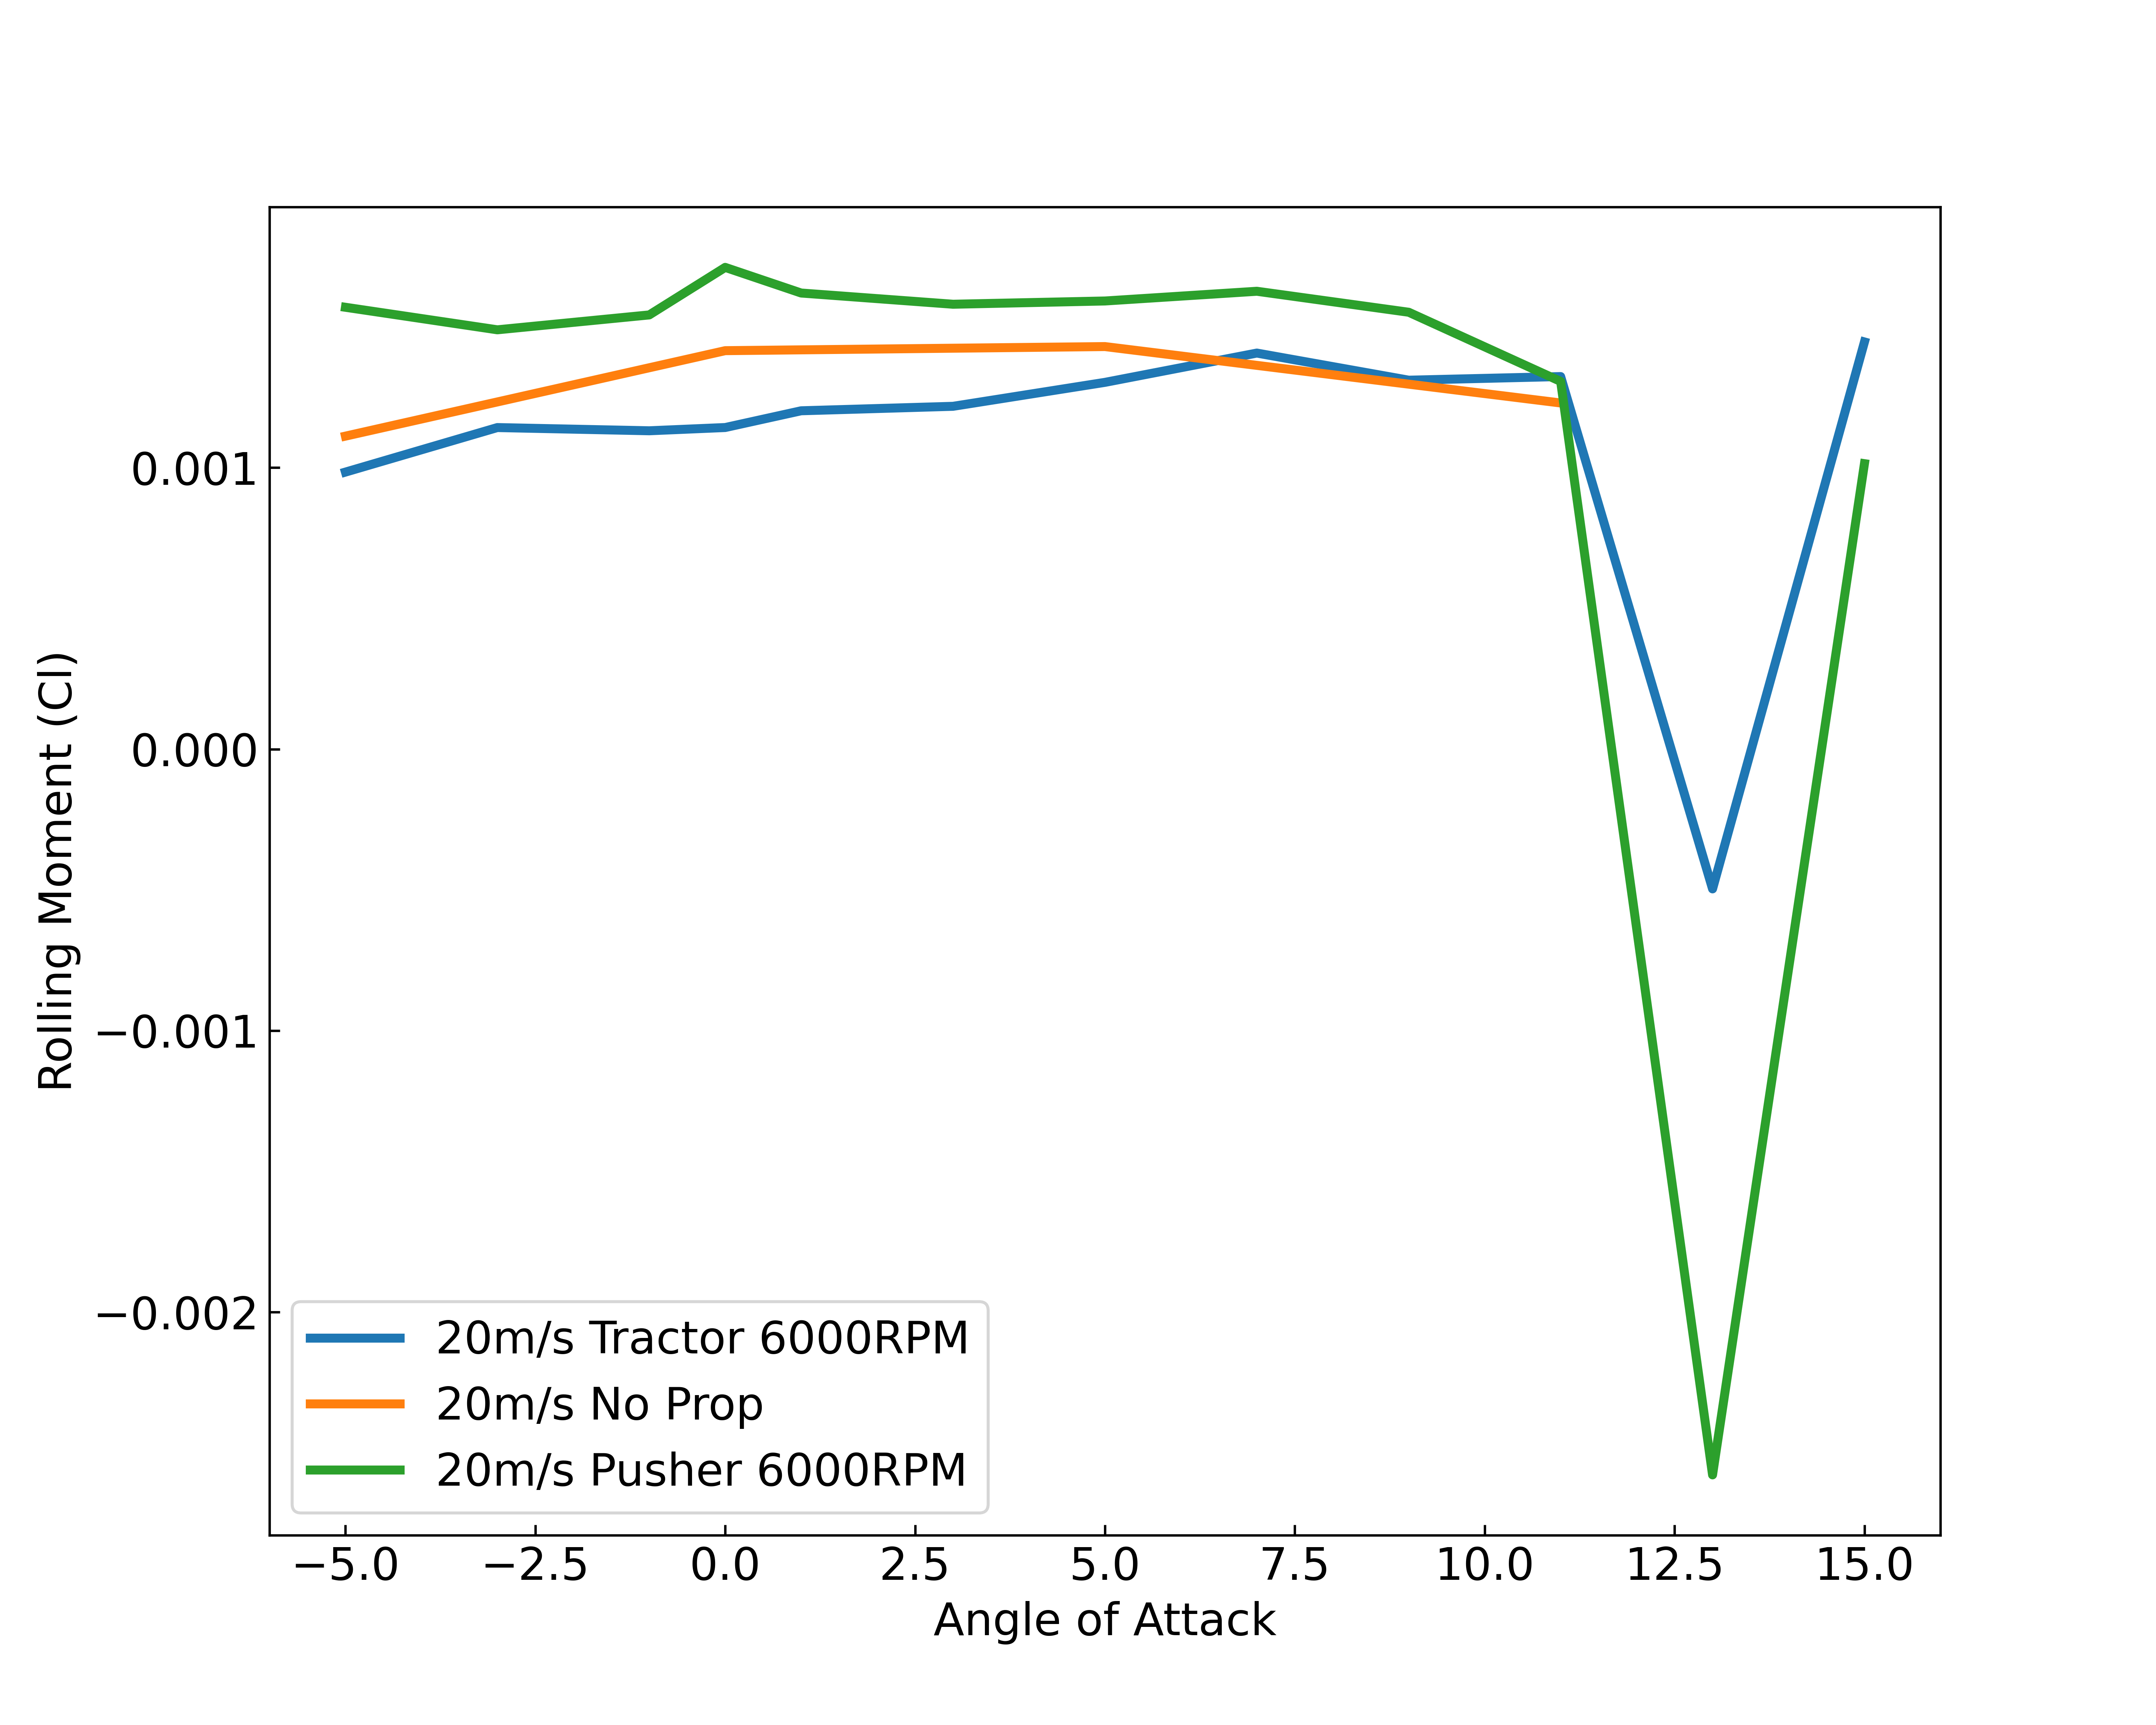
\includegraphics[width=\textwidth]{05_Results/Figs/Cl_roll/20ms_6000RPM_Cl_roll.png}
        \caption{Rolling Moment Coefficient at 20m/s airspeed and 6000RPM motor speed}
        \label{fig:Cl_roll_20ms_6000}
    \end{subfigure}
    \begin{subfigure}[b]{0.467\textwidth}
        \centering
        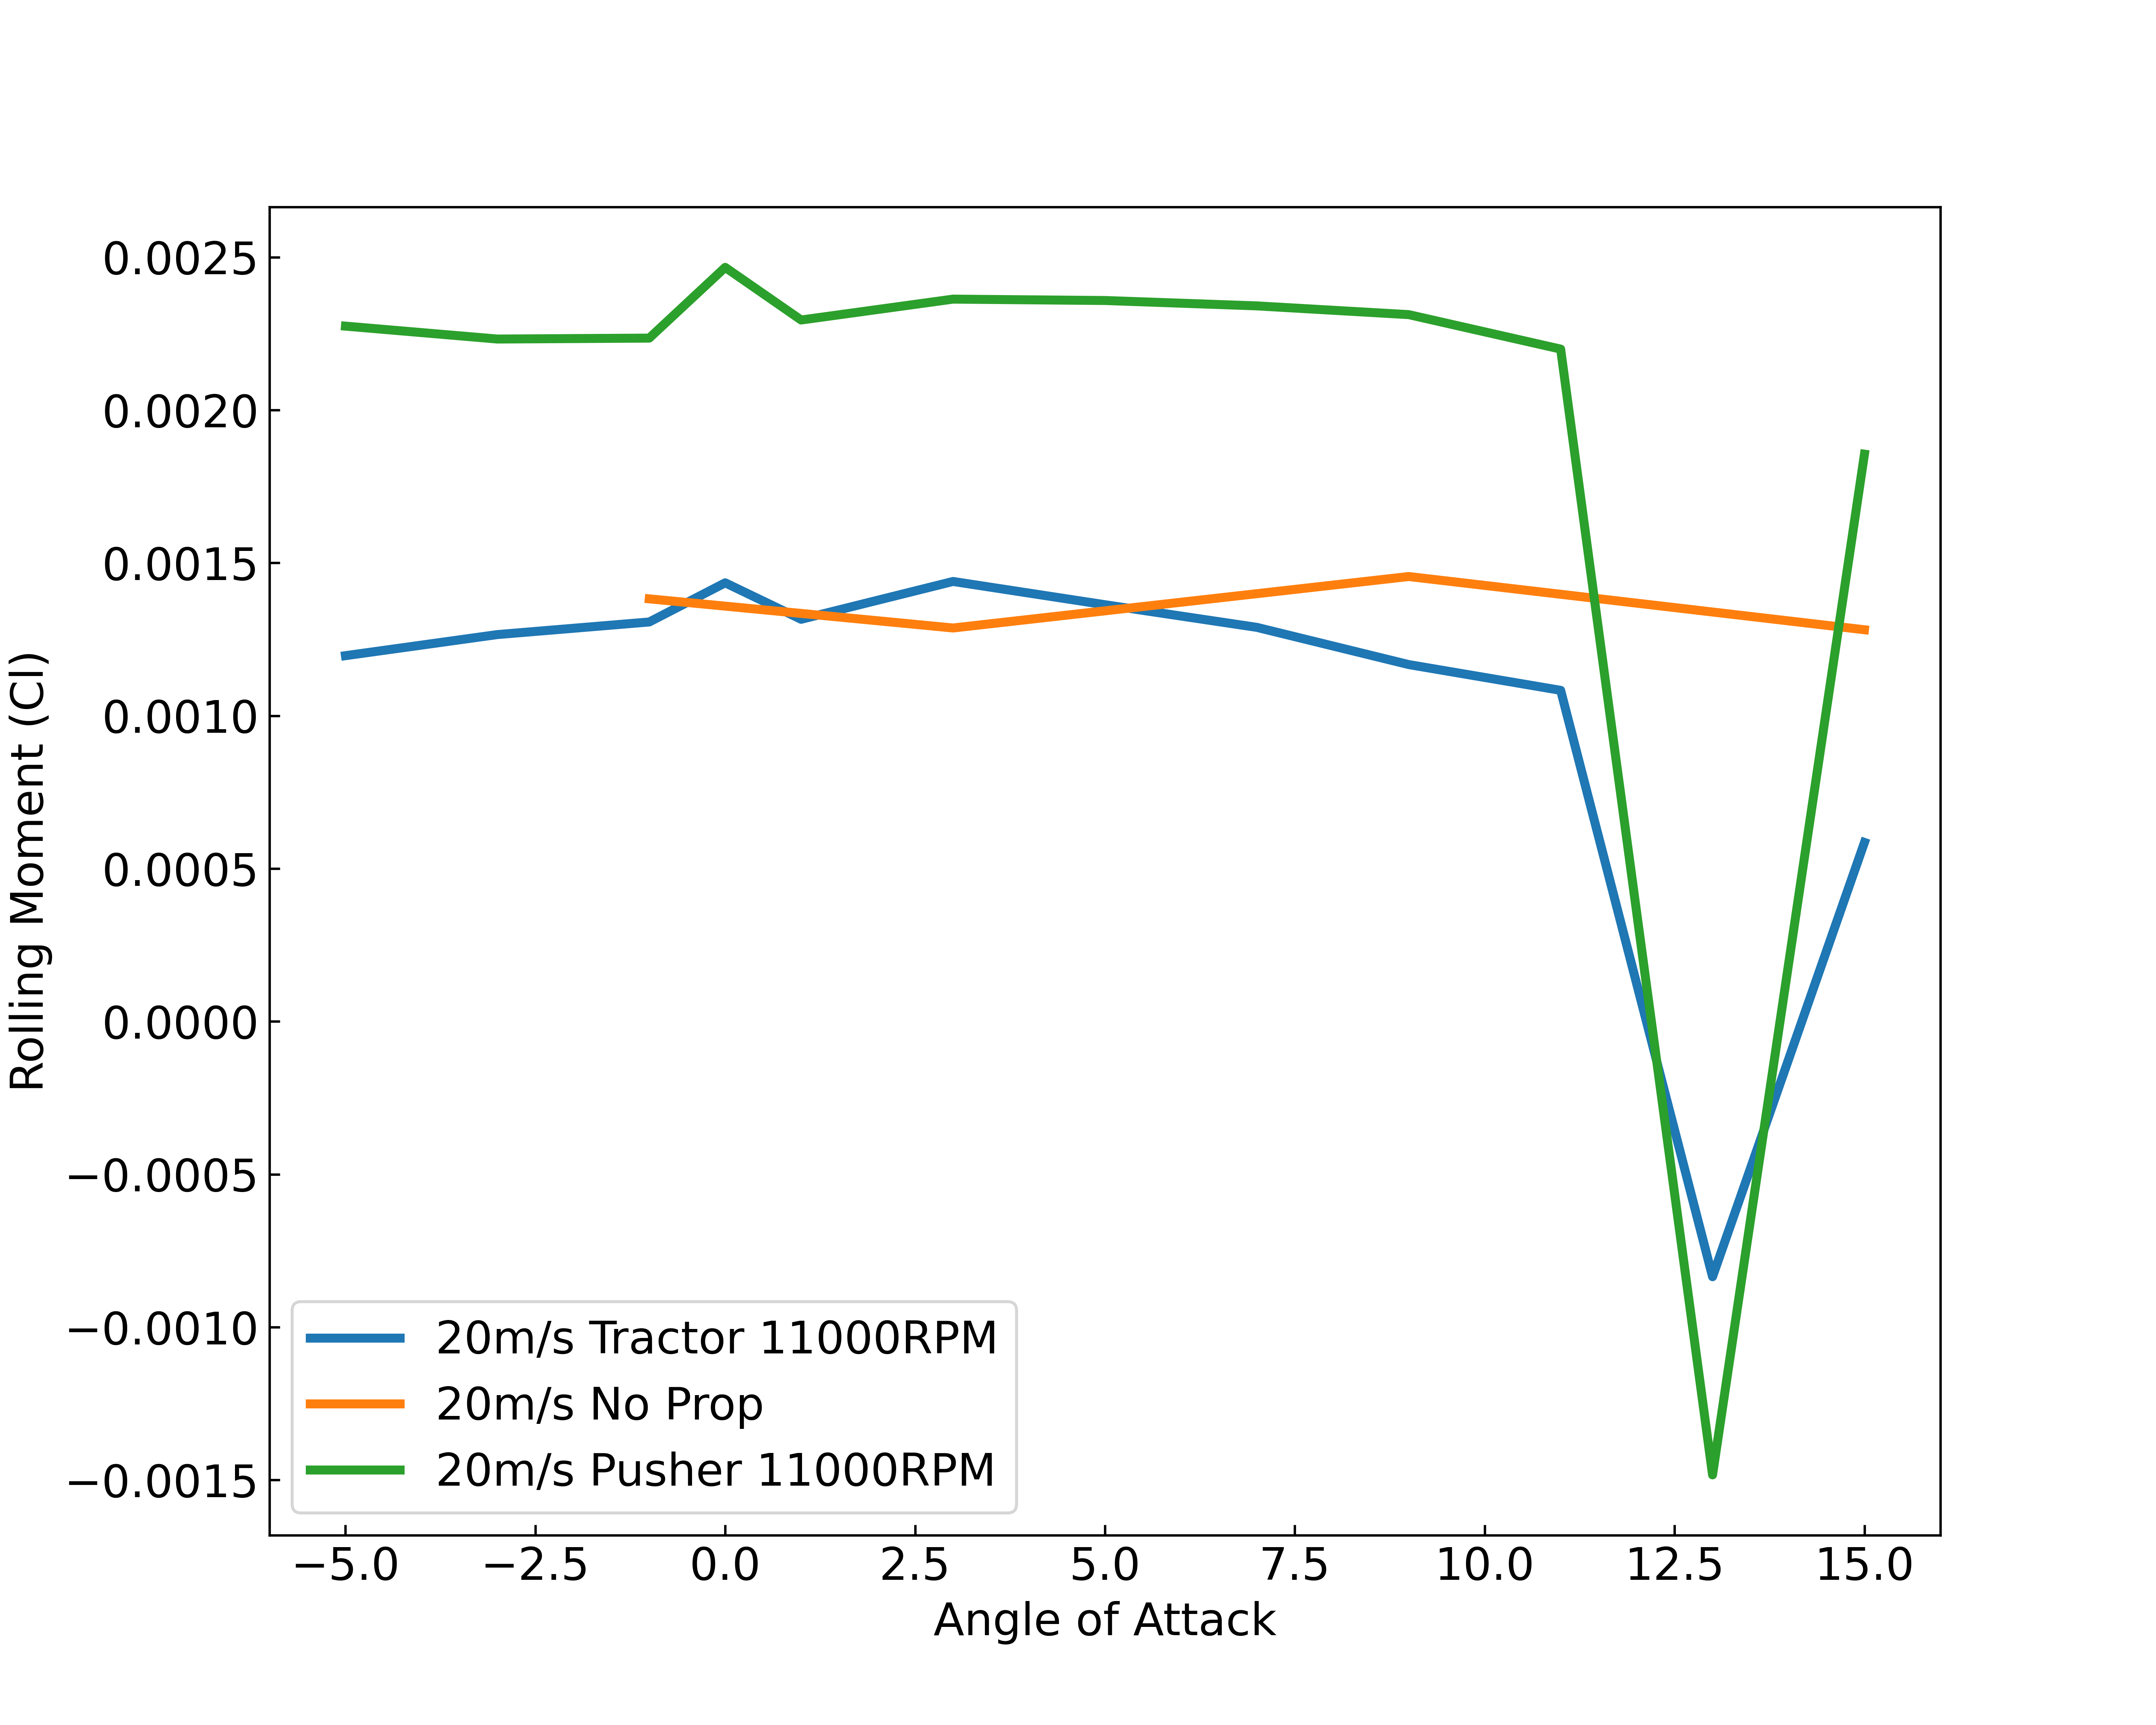
\includegraphics[width=\textwidth]{05_Results/Figs/Cl_roll/20ms_11000RPM_Cl.png}
        \caption{Rolling Moment Coefficient at 20m/s airspeed and 11000RPM motor speed}
        \label{fig:Cl_roll_20ms_11000}
    \end{subfigure}
\end{figure}

\subsection{Static Margin}

\todo{Add table with values of static margin}
\begin{figure}[H]
    \centering
    \begin{subfigure}[b]{0.467\textwidth}
        \centering
        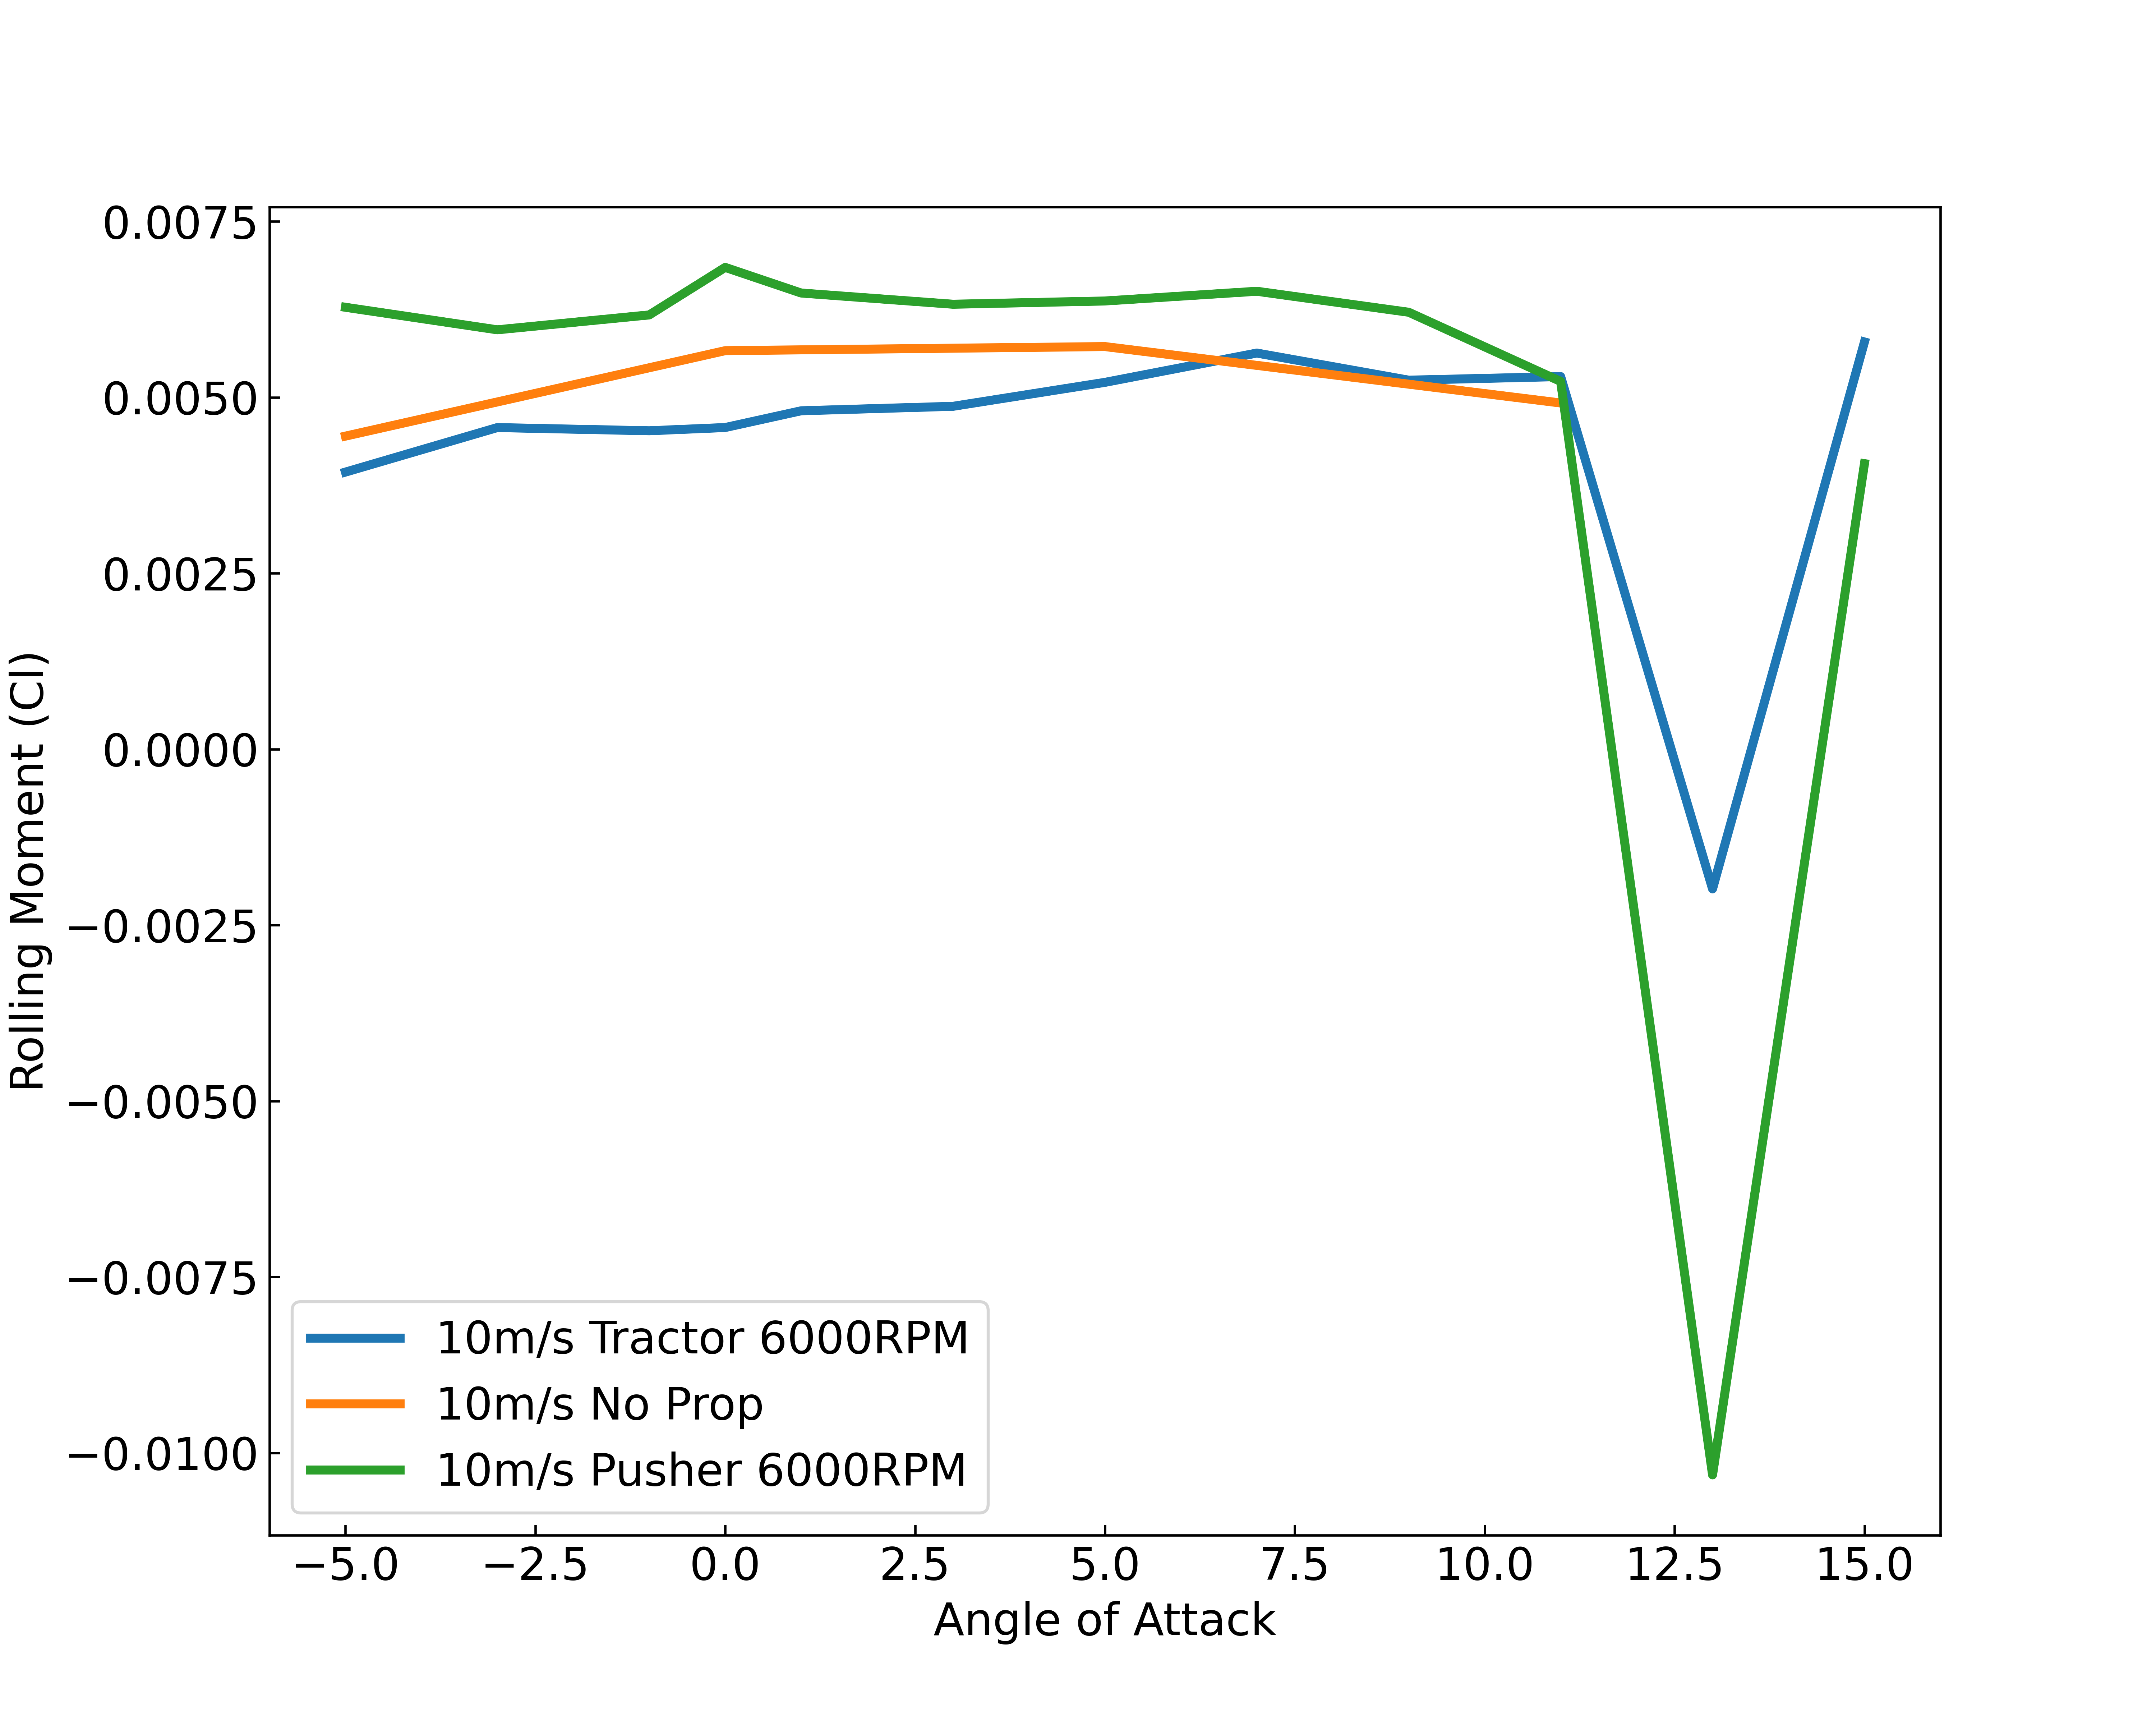
\includegraphics[width=\textwidth]{05_Results/Figs/Cl_roll/10ms_6000RPM_Cl_roll.png}
        \caption{Rolling Moment Coefficient at 10m/s airspeed and 6000RPM motor speed}
        \label{fig:CmCl_10ms_6000}
    \end{subfigure}
    \begin{subfigure}[b]{0.467\textwidth}
        \centering
        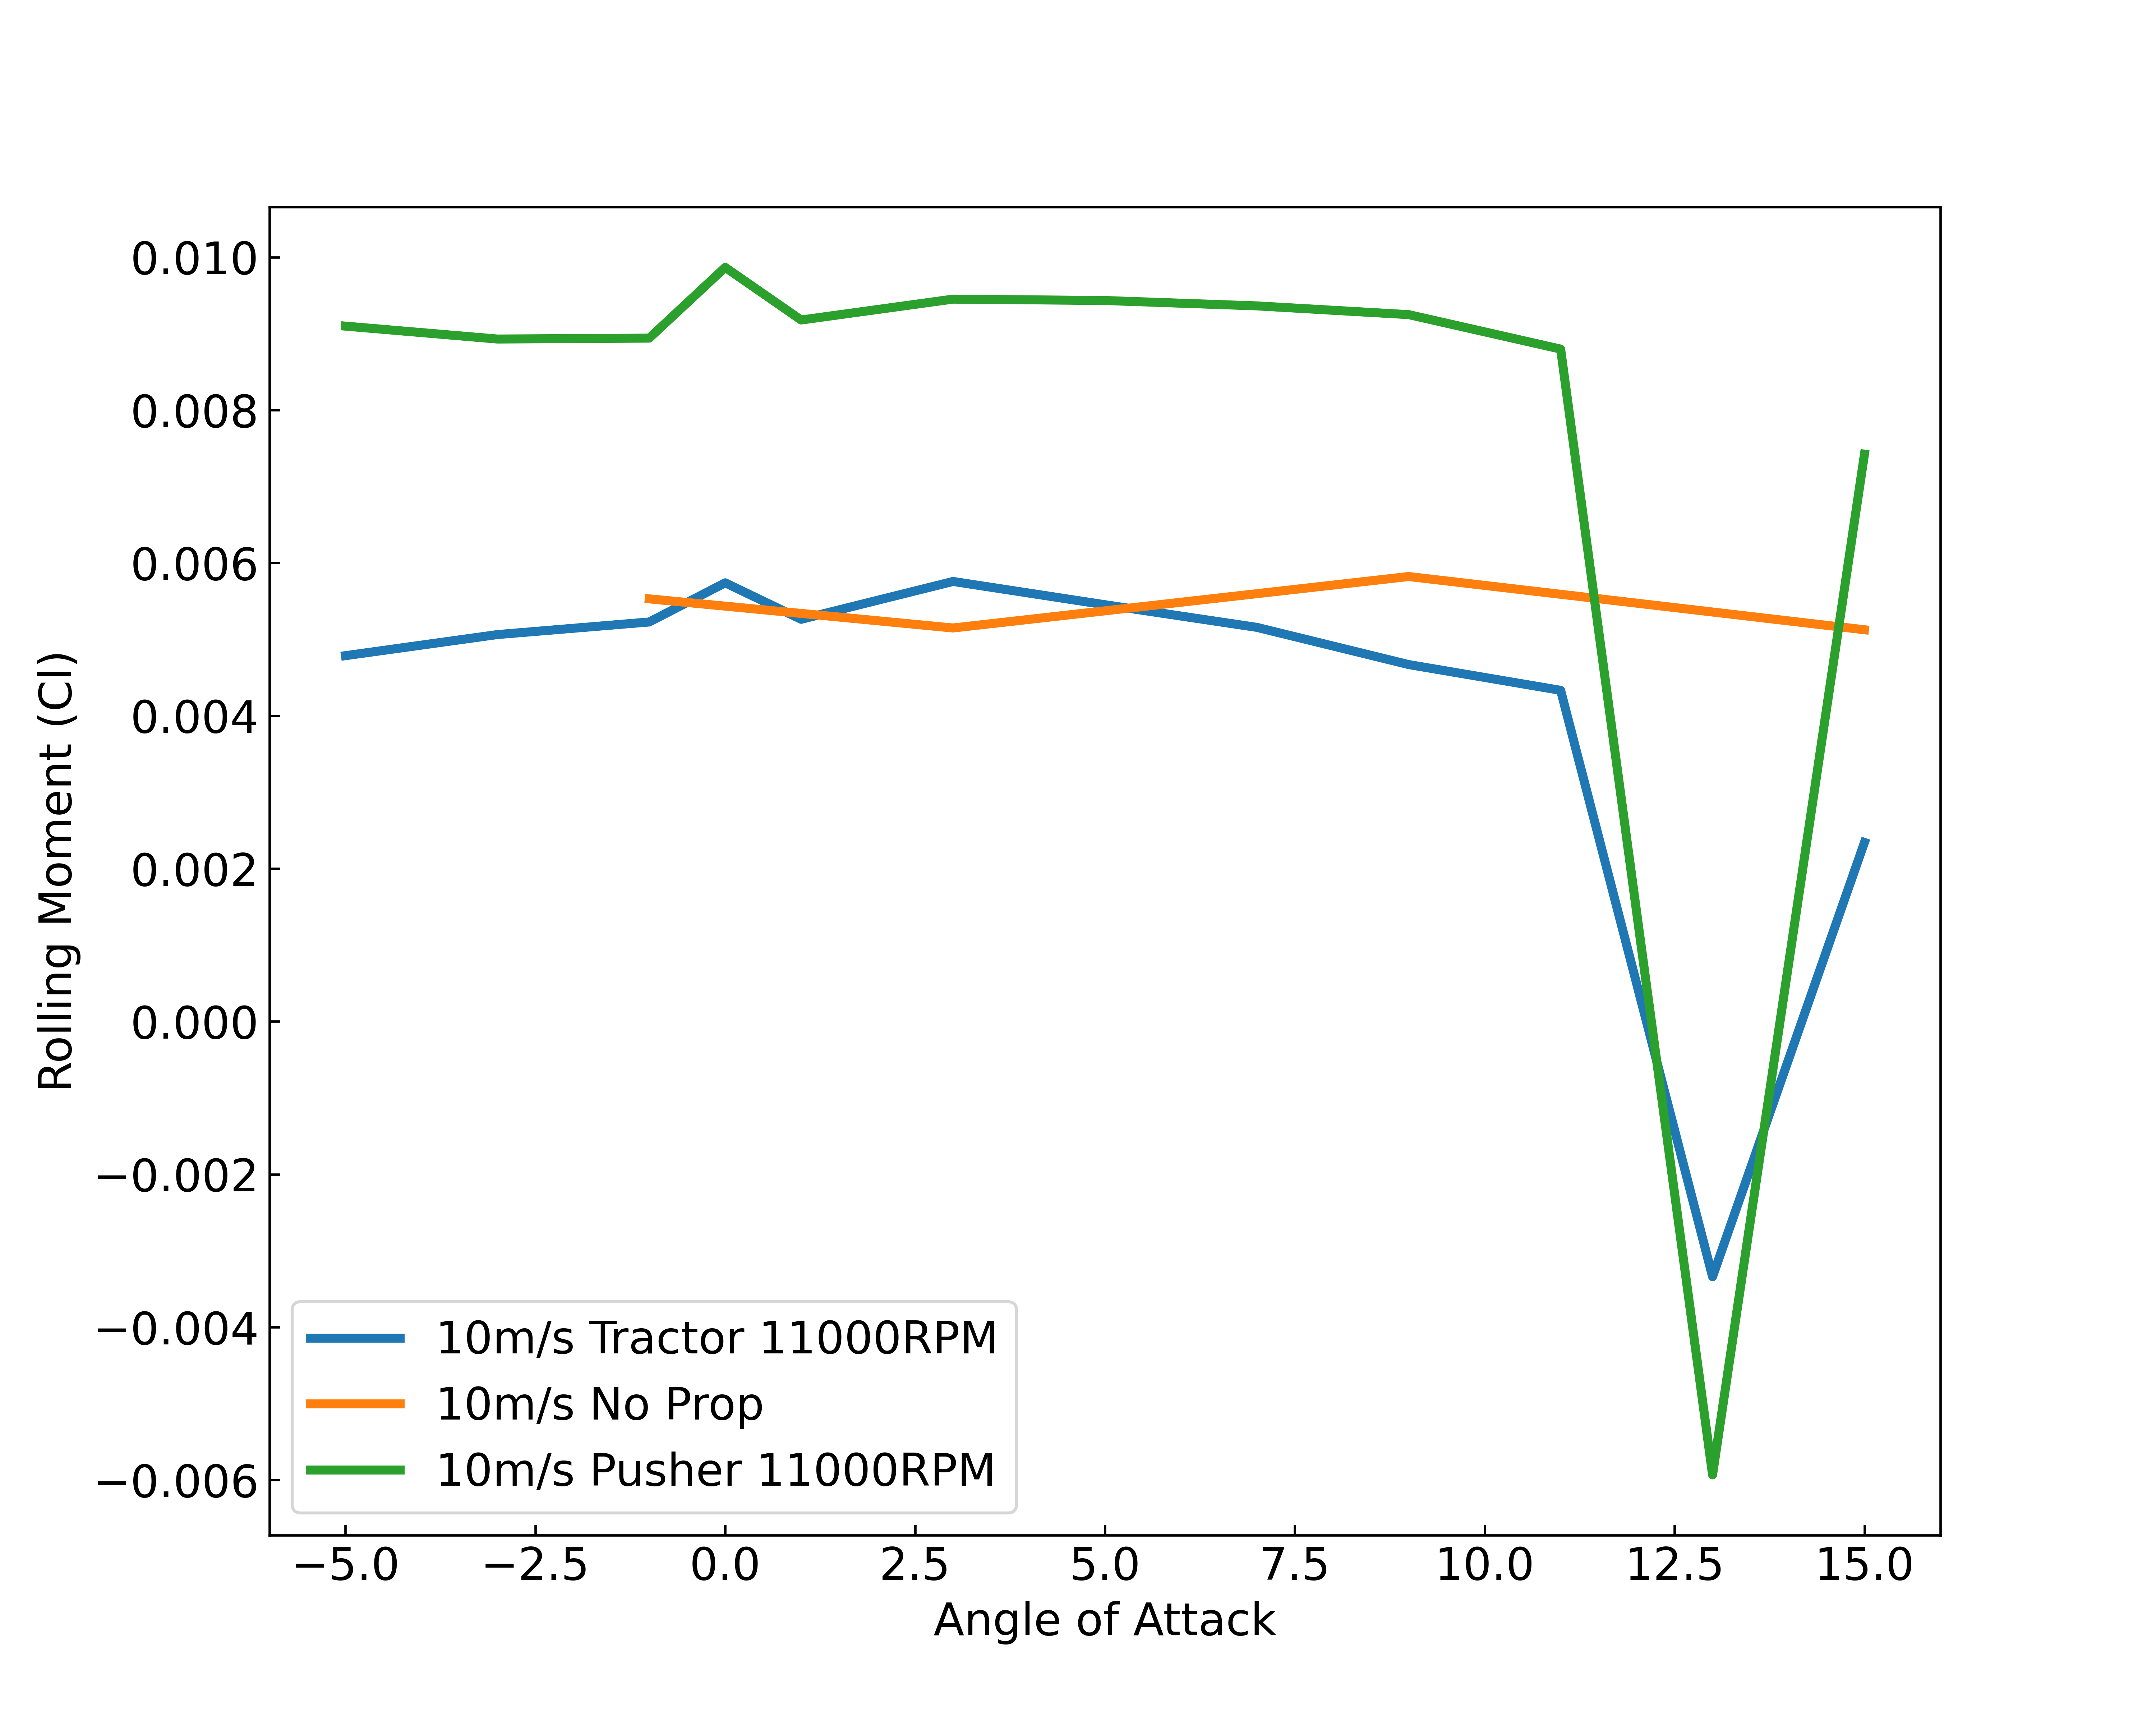
\includegraphics[width=\textwidth]{05_Results/Figs/Cl_roll/10ms_11000RPM_Cl.png}
        \caption{Rolling Moment Coefficient at 10m/s airspeed and 11000RPM motor speed}
        \label{fig:CmCl_10ms_11000}
    \end{subfigure}
    \begin{subfigure}[b]{0.467\textwidth}
        \centering
        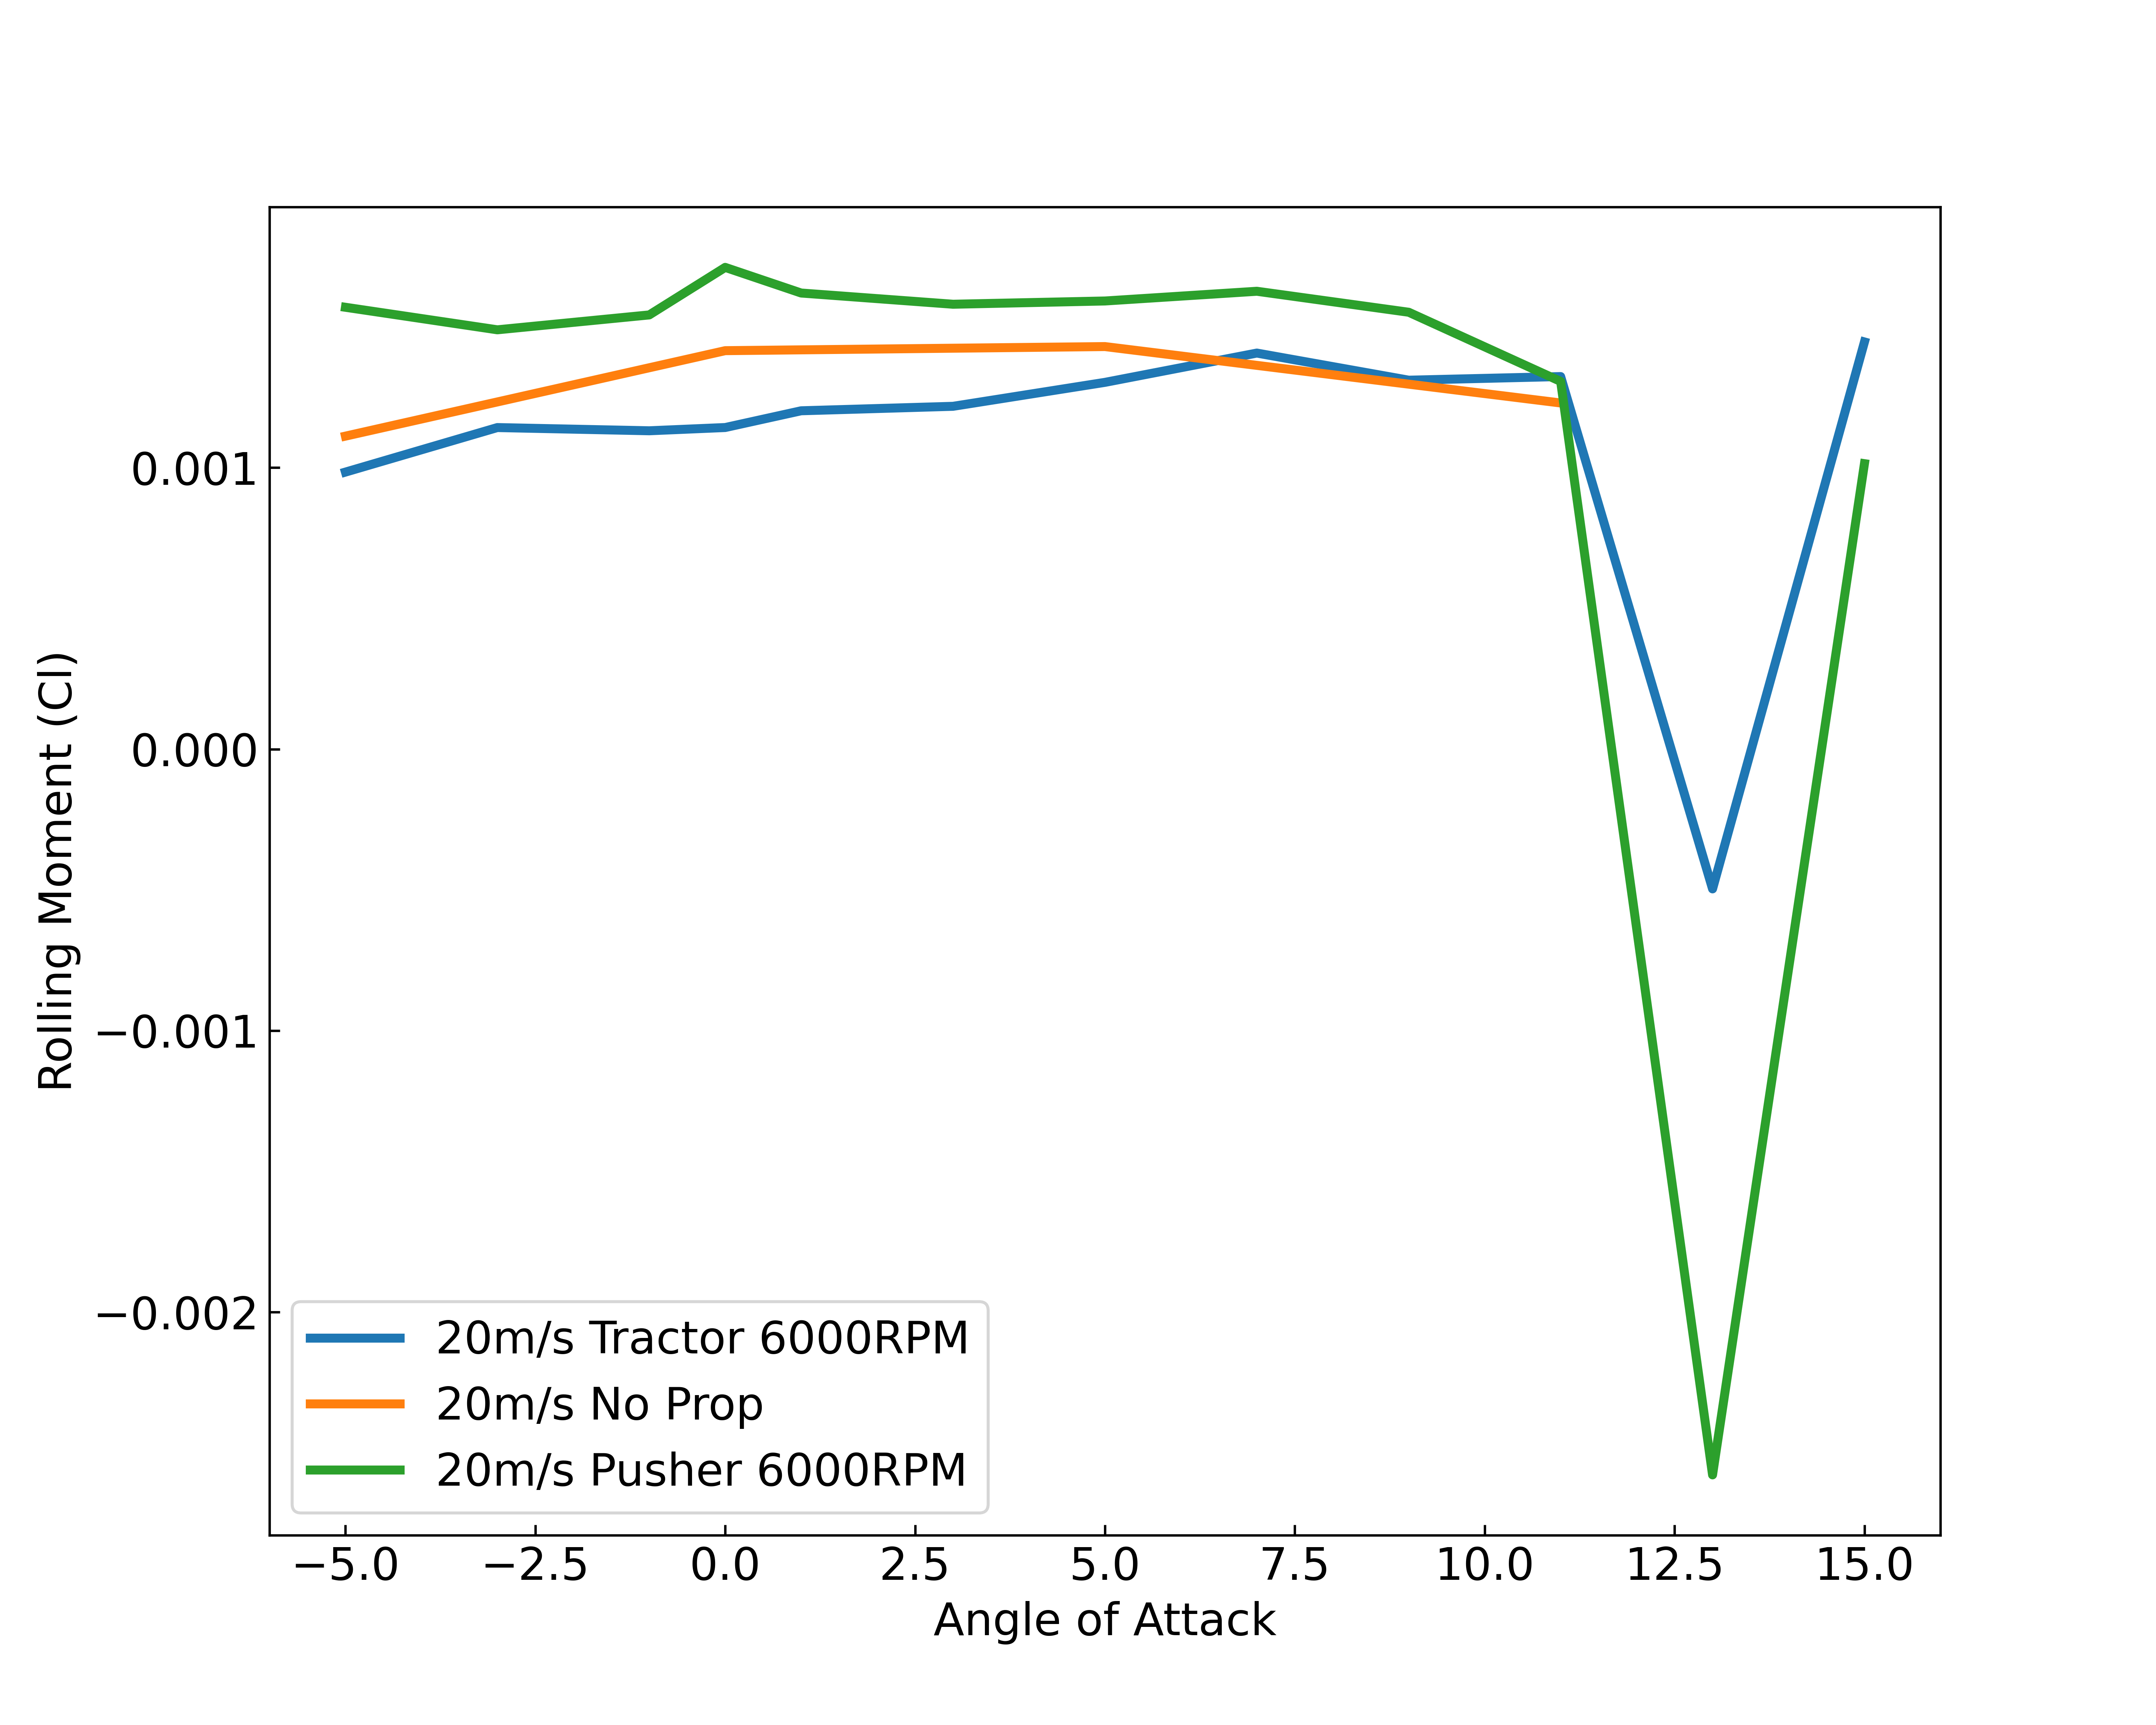
\includegraphics[width=\textwidth]{05_Results/Figs/Cl_roll/20ms_6000RPM_Cl_roll.png}
        \caption{Rolling Moment Coefficient at 20m/s airspeed and 6000RPM motor speed}
        \label{fig:CmCl_20ms_6000}
    \end{subfigure}
    \begin{subfigure}[b]{0.467\textwidth}
        \centering
        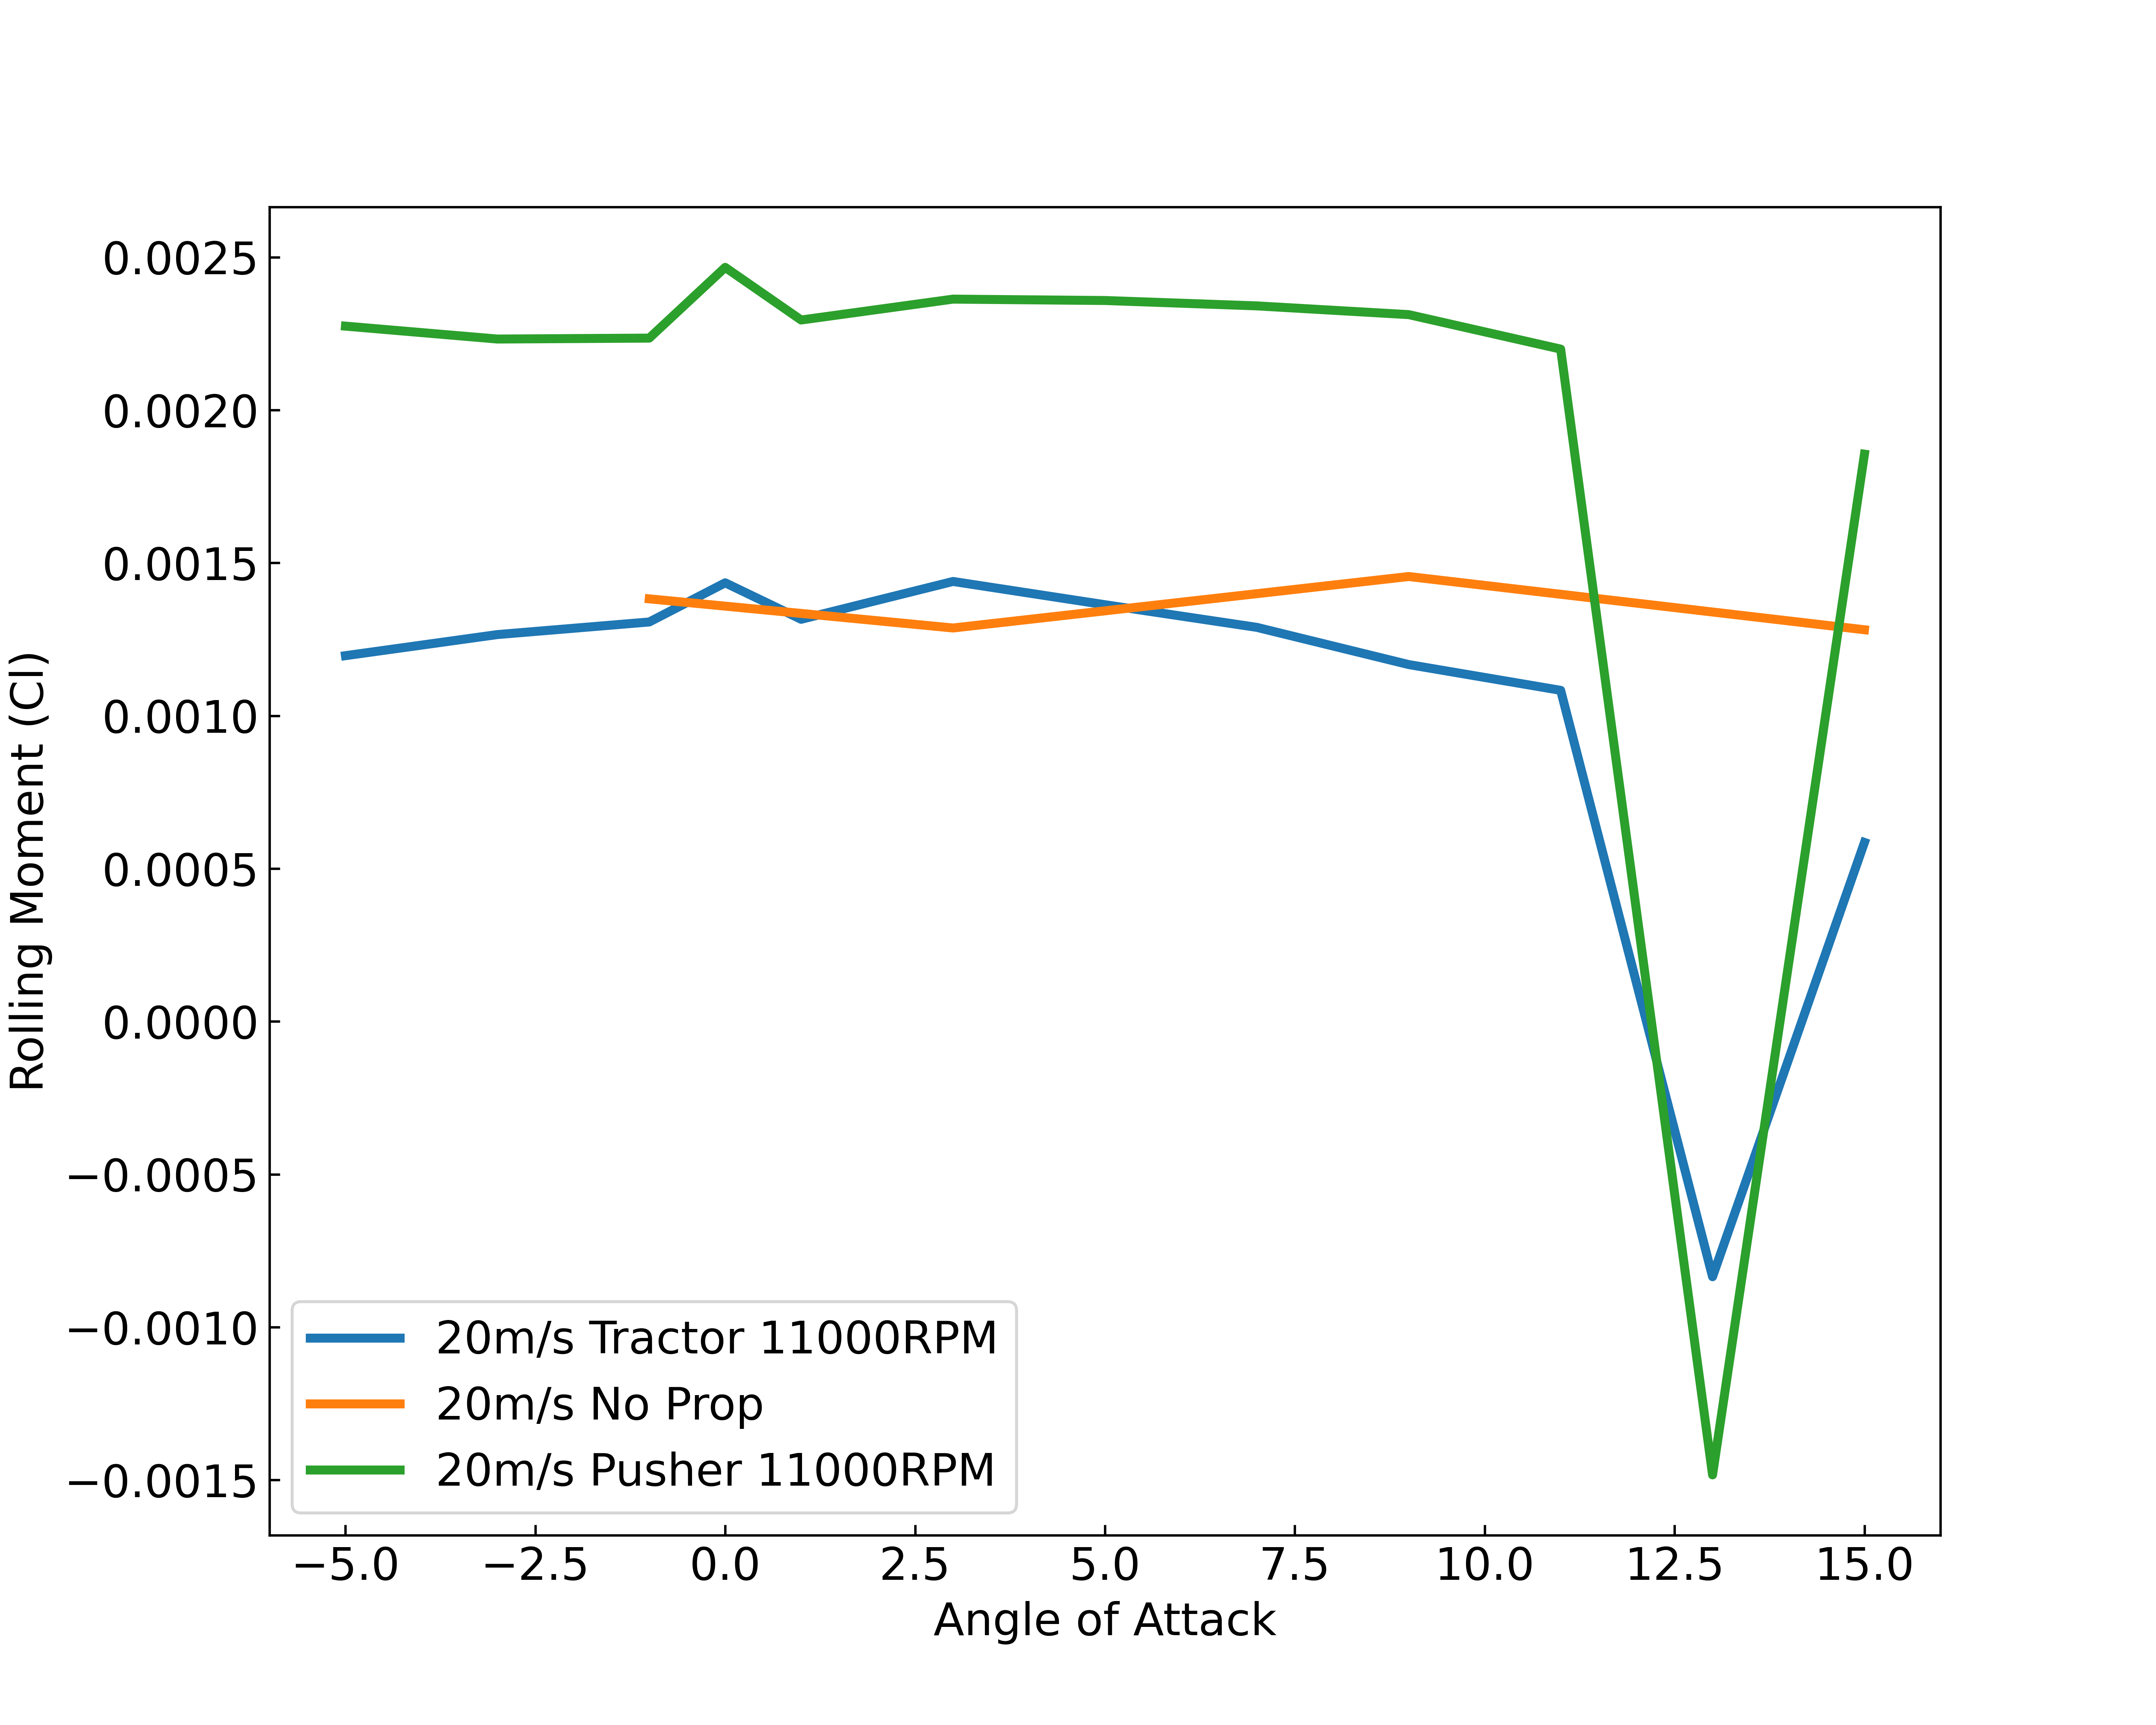
\includegraphics[width=\textwidth]{05_Results/Figs/Cl_roll/20ms_11000RPM_Cl.png}
        \caption{Rolling Moment Coefficient at 20m/s airspeed and 11000RPM motor speed}
        \label{fig:CmCl_20ms_11000}
    \end{subfigure}
\end{figure}


\section{VAP Validation}

\subsection{Wing Validation}


\begin{figure}[H]
     \centering
     \begin{subfigure}[b]{0.45\textwidth}
         \centering
         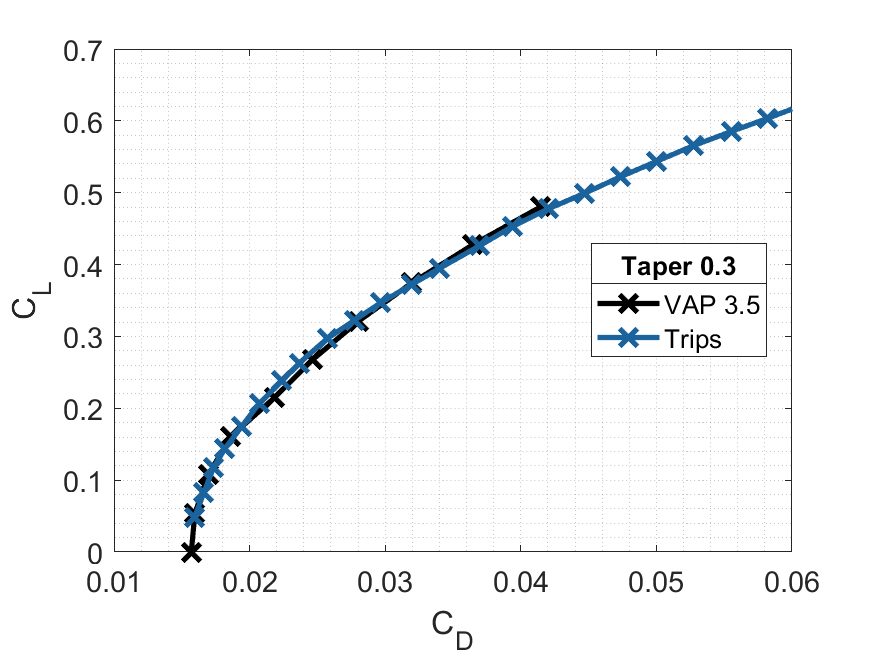
\includegraphics[width=\textwidth]{05_Results/Figs/VAP/genMAV/taper3a.png}

     \end{subfigure}
     \hfill
     \begin{subfigure}[b]{0.45\textwidth}
         \centering
         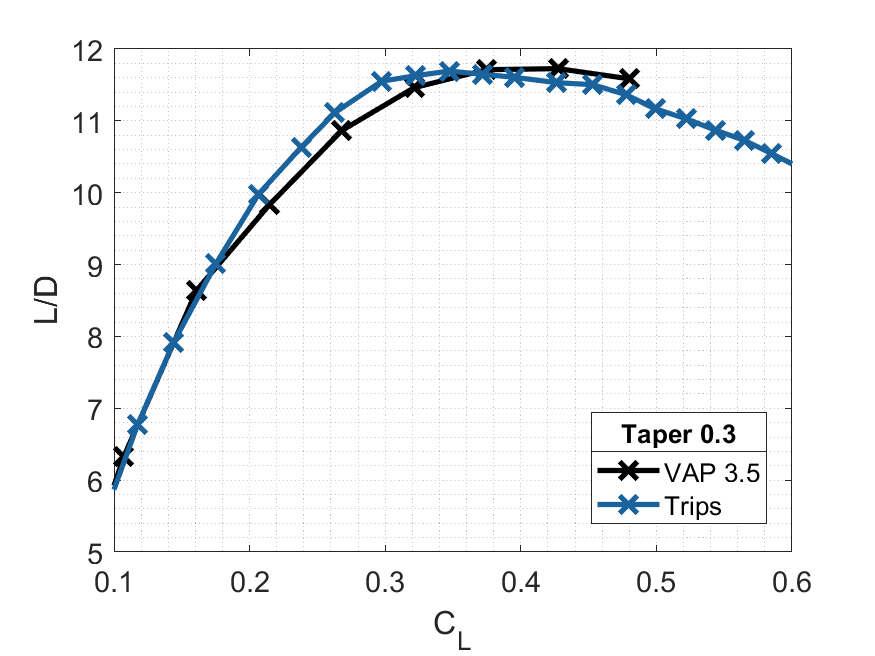
\includegraphics[width=\textwidth]{05_Results/Figs/VAP/genMAV/taper3b.png}
      
     \end{subfigure}
     \hfill

        
\end{figure}


\begin{figure}[H]
     \centering
     \begin{subfigure}[b]{0.45\textwidth}
         \centering
         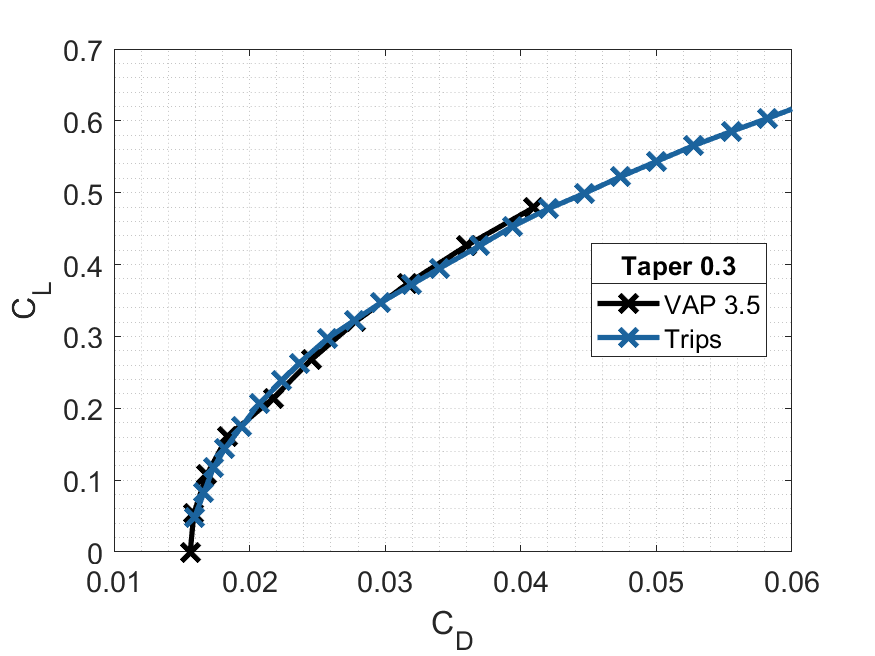
\includegraphics[width=\textwidth]{05_Results/Figs/VAP/genMAV/taper5a.png}

     \end{subfigure}
     \hfill
     \begin{subfigure}[b]{0.45\textwidth}
         \centering
         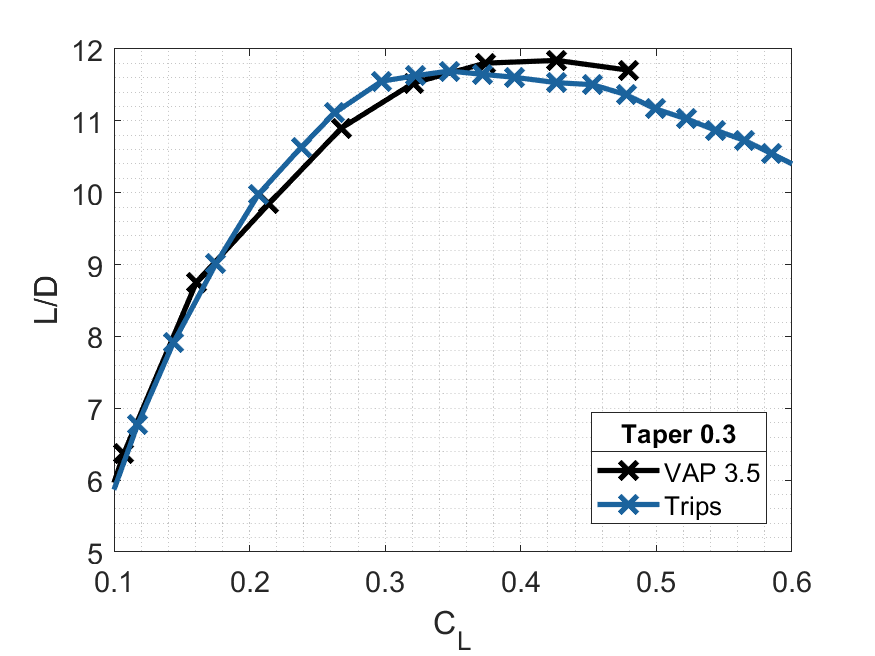
\includegraphics[width=\textwidth]{05_Results/Figs/VAP/genMAV/taper5b.png}
      
     \end{subfigure}
     \hfill

        
\end{figure}


\begin{figure}[H]
     \centering
     \begin{subfigure}[b]{0.45\textwidth}
         \centering
         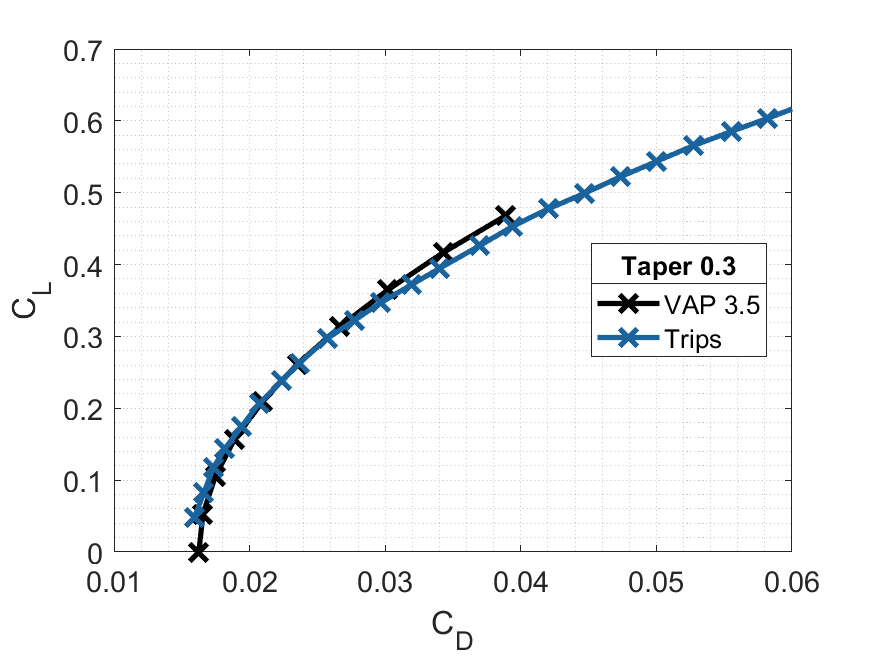
\includegraphics[width=\textwidth]{05_Results/Figs/VAP/genMAV/taper10a.png}

     \end{subfigure}
     \hfill
     \begin{subfigure}[b]{0.45\textwidth}
         \centering
         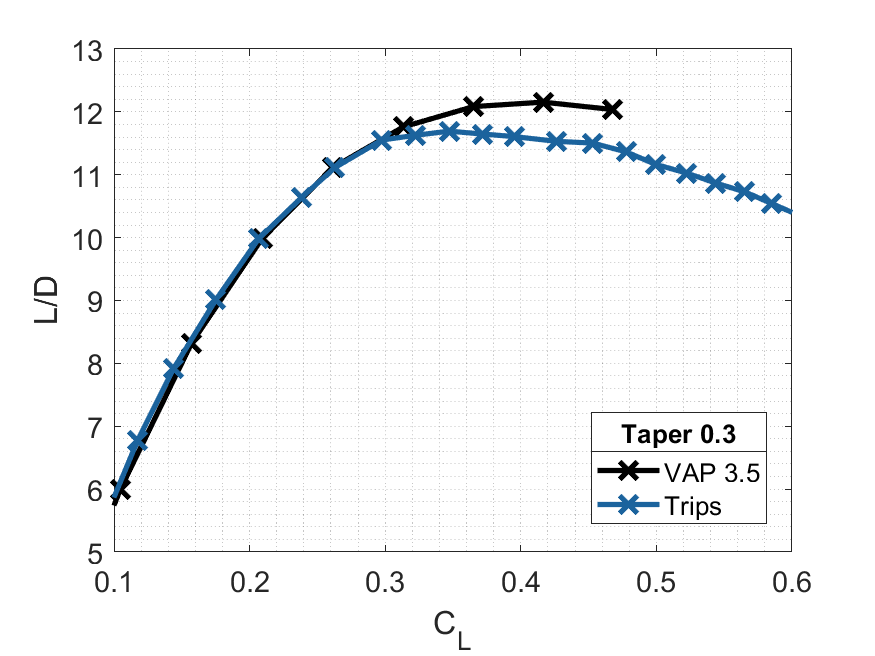
\includegraphics[width=\textwidth]{05_Results/Figs/VAP/genMAV/taper10b.png}
      
     \end{subfigure}
     \hfill

        
\end{figure}


\subsection{GenMAV model validation}


\begin{figure}[H]
     \centering
     \begin{subfigure}[b]{0.45\textwidth}
          \centering
        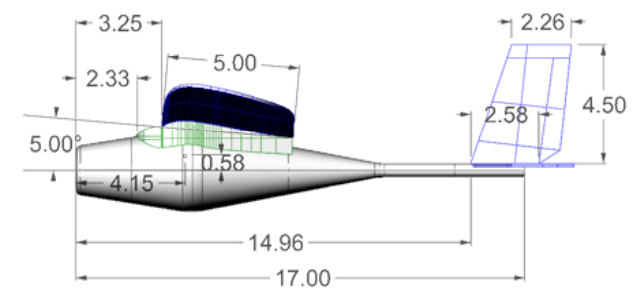
\includegraphics[width=0.5\textwidth]{05_Results/Figs/VAP/genMAV/dimensions.png}
            \label{fig:genMAVDimensions}

     \end{subfigure}
     \hfill
     \begin{subfigure}[b]{0.45\textwidth}
                \centering
            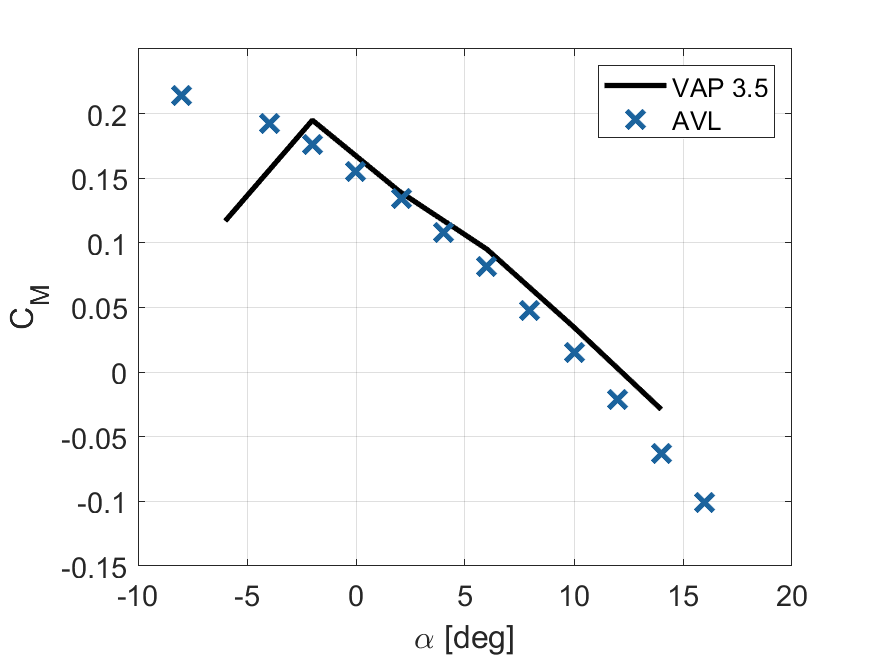
\includegraphics[width=0.5\textwidth]{05_Results/Figs/VAP/genMAV/GenMAVModelValidation1.png}
             \label{fig:genMAV_Cm}
              \caption{}
     \end{subfigure}
     \hfill

        
\end{figure}


\begin{figure}[H]
     \centering
     \begin{subfigure}[b]{0.45\textwidth}
            \centering
         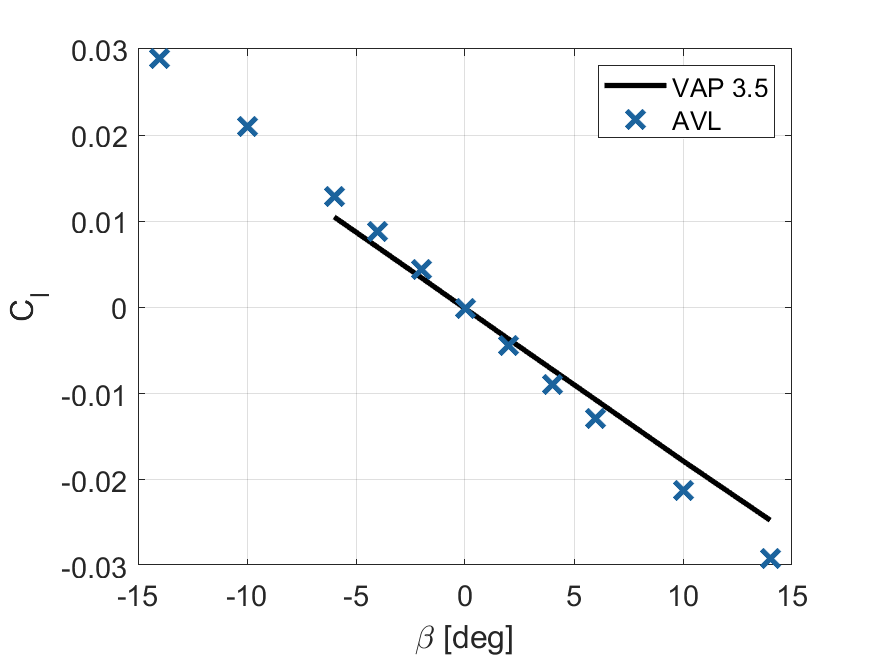
\includegraphics[width=0.5\textwidth]{05_Results/Figs/VAP/genMAV/GenMAVModelValidation2.png}
         \label{fig:genMAV_Cl_roll}
         \caption{}

     \end{subfigure}
     \hfill
     \begin{subfigure}[b]{0.45\textwidth}
               \centering
         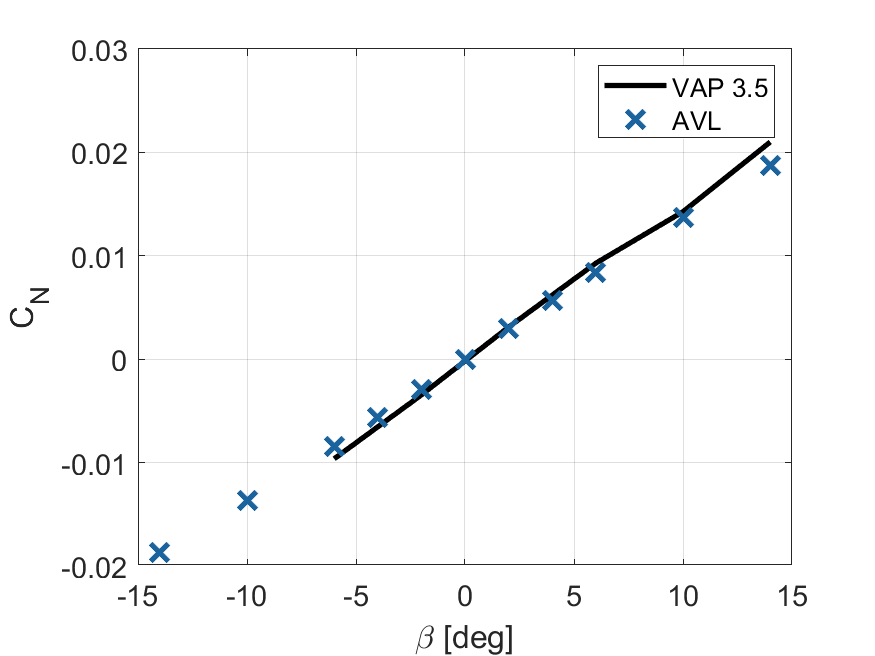
\includegraphics[width=0.5\textwidth]{05_Results/Figs/VAP/genMAV/GenMAVModelValidation3.png}
         \label{fig:genMAV_Cn}
         \caption{}
     \end{subfigure}
     \hfill
\end{figure}



% \begin{figure}[H]
%     \centering
%     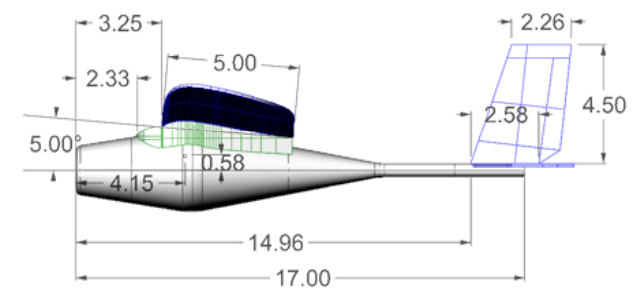
\includegraphics[width=0.5\textwidth]{05_Results/Figs/VAP/genMAV/dimensions.png}
%     \label{fig:genMAVDimensions}
% \end{figure}

% \begin{figure}[H]
%          \centering
%          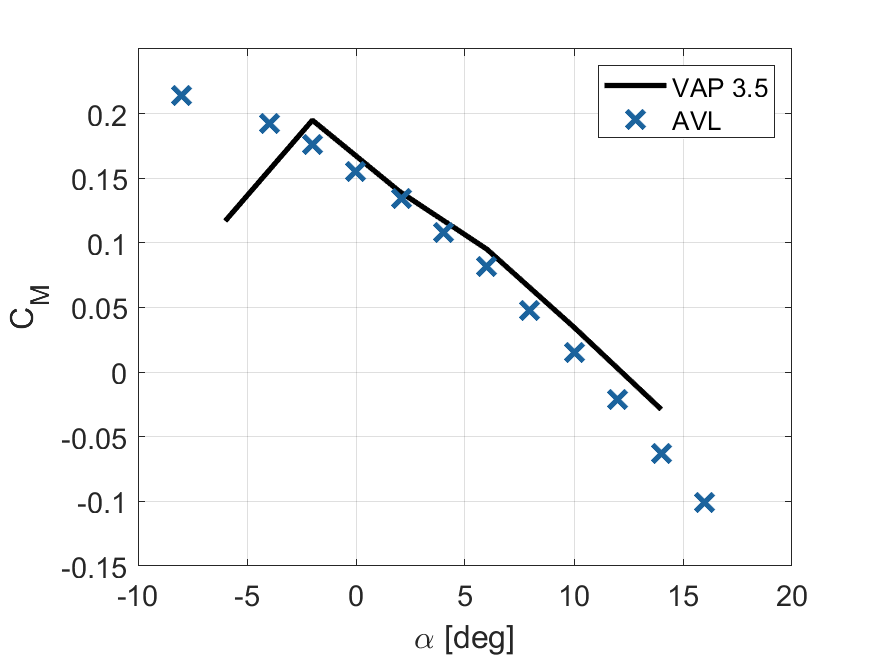
\includegraphics[width=0.5\textwidth]{05_Results/Figs/VAP/genMAV/GenMAVModelValidation1.png}
%          \label{fig:genMAV_Cm}
%          \caption{}
% \end{figure}

% \begin{figure}[H]
       
% \end{figure}

% \begin{figure}
       
% \end{figure}

\subsection{Validation of Wind Tunnel Results with VAP}


\subsubsection{No Propeller Configuration}


\begin{figure}[H]
    \centering
    \begin{subfigure}[b]{0.467\textwidth}
        \centering
        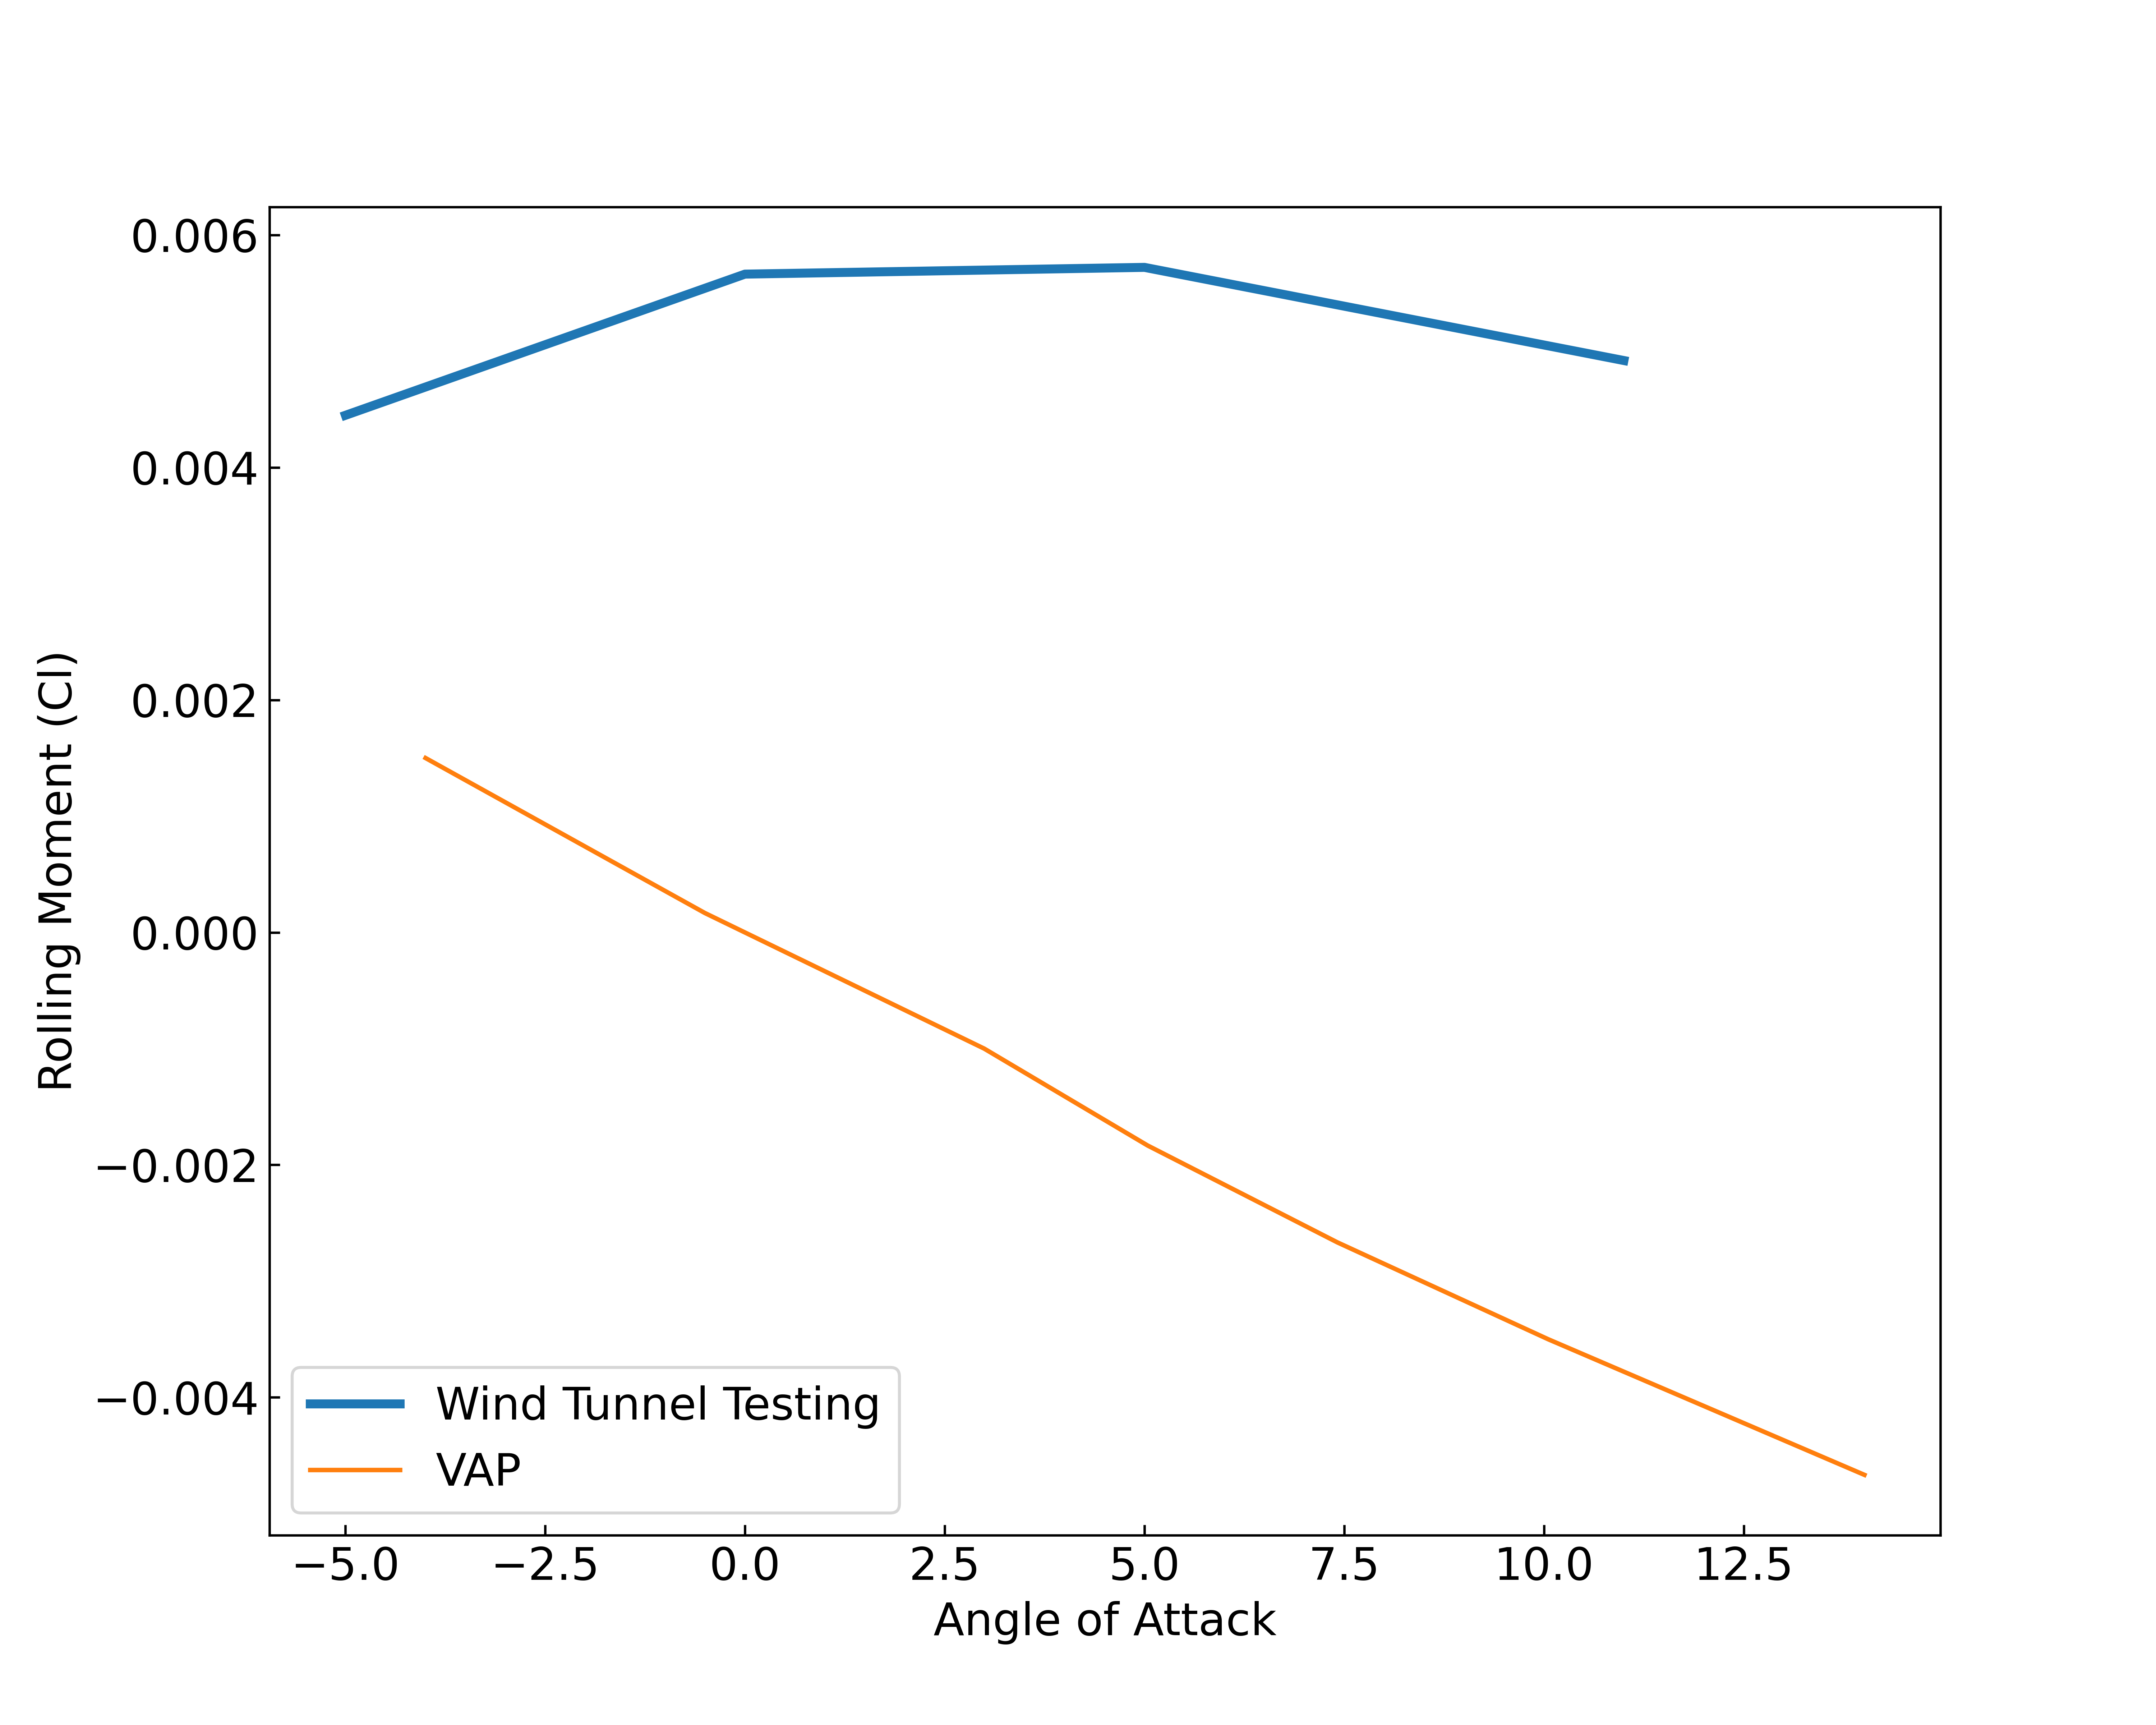
\includegraphics[width=\textwidth]{05_Results/VAP/noProp/Cl/10ms_6000RPM_Cl.png}
        \caption{Rolling Moment Coefficient at 10m/s airspeed and 6000RPM motor speed}
        \label{fig:VAP_NoProp_Cl_10ms_6000}
    \end{subfigure}
    \begin{subfigure}[b]{0.467\textwidth}
        \centering
        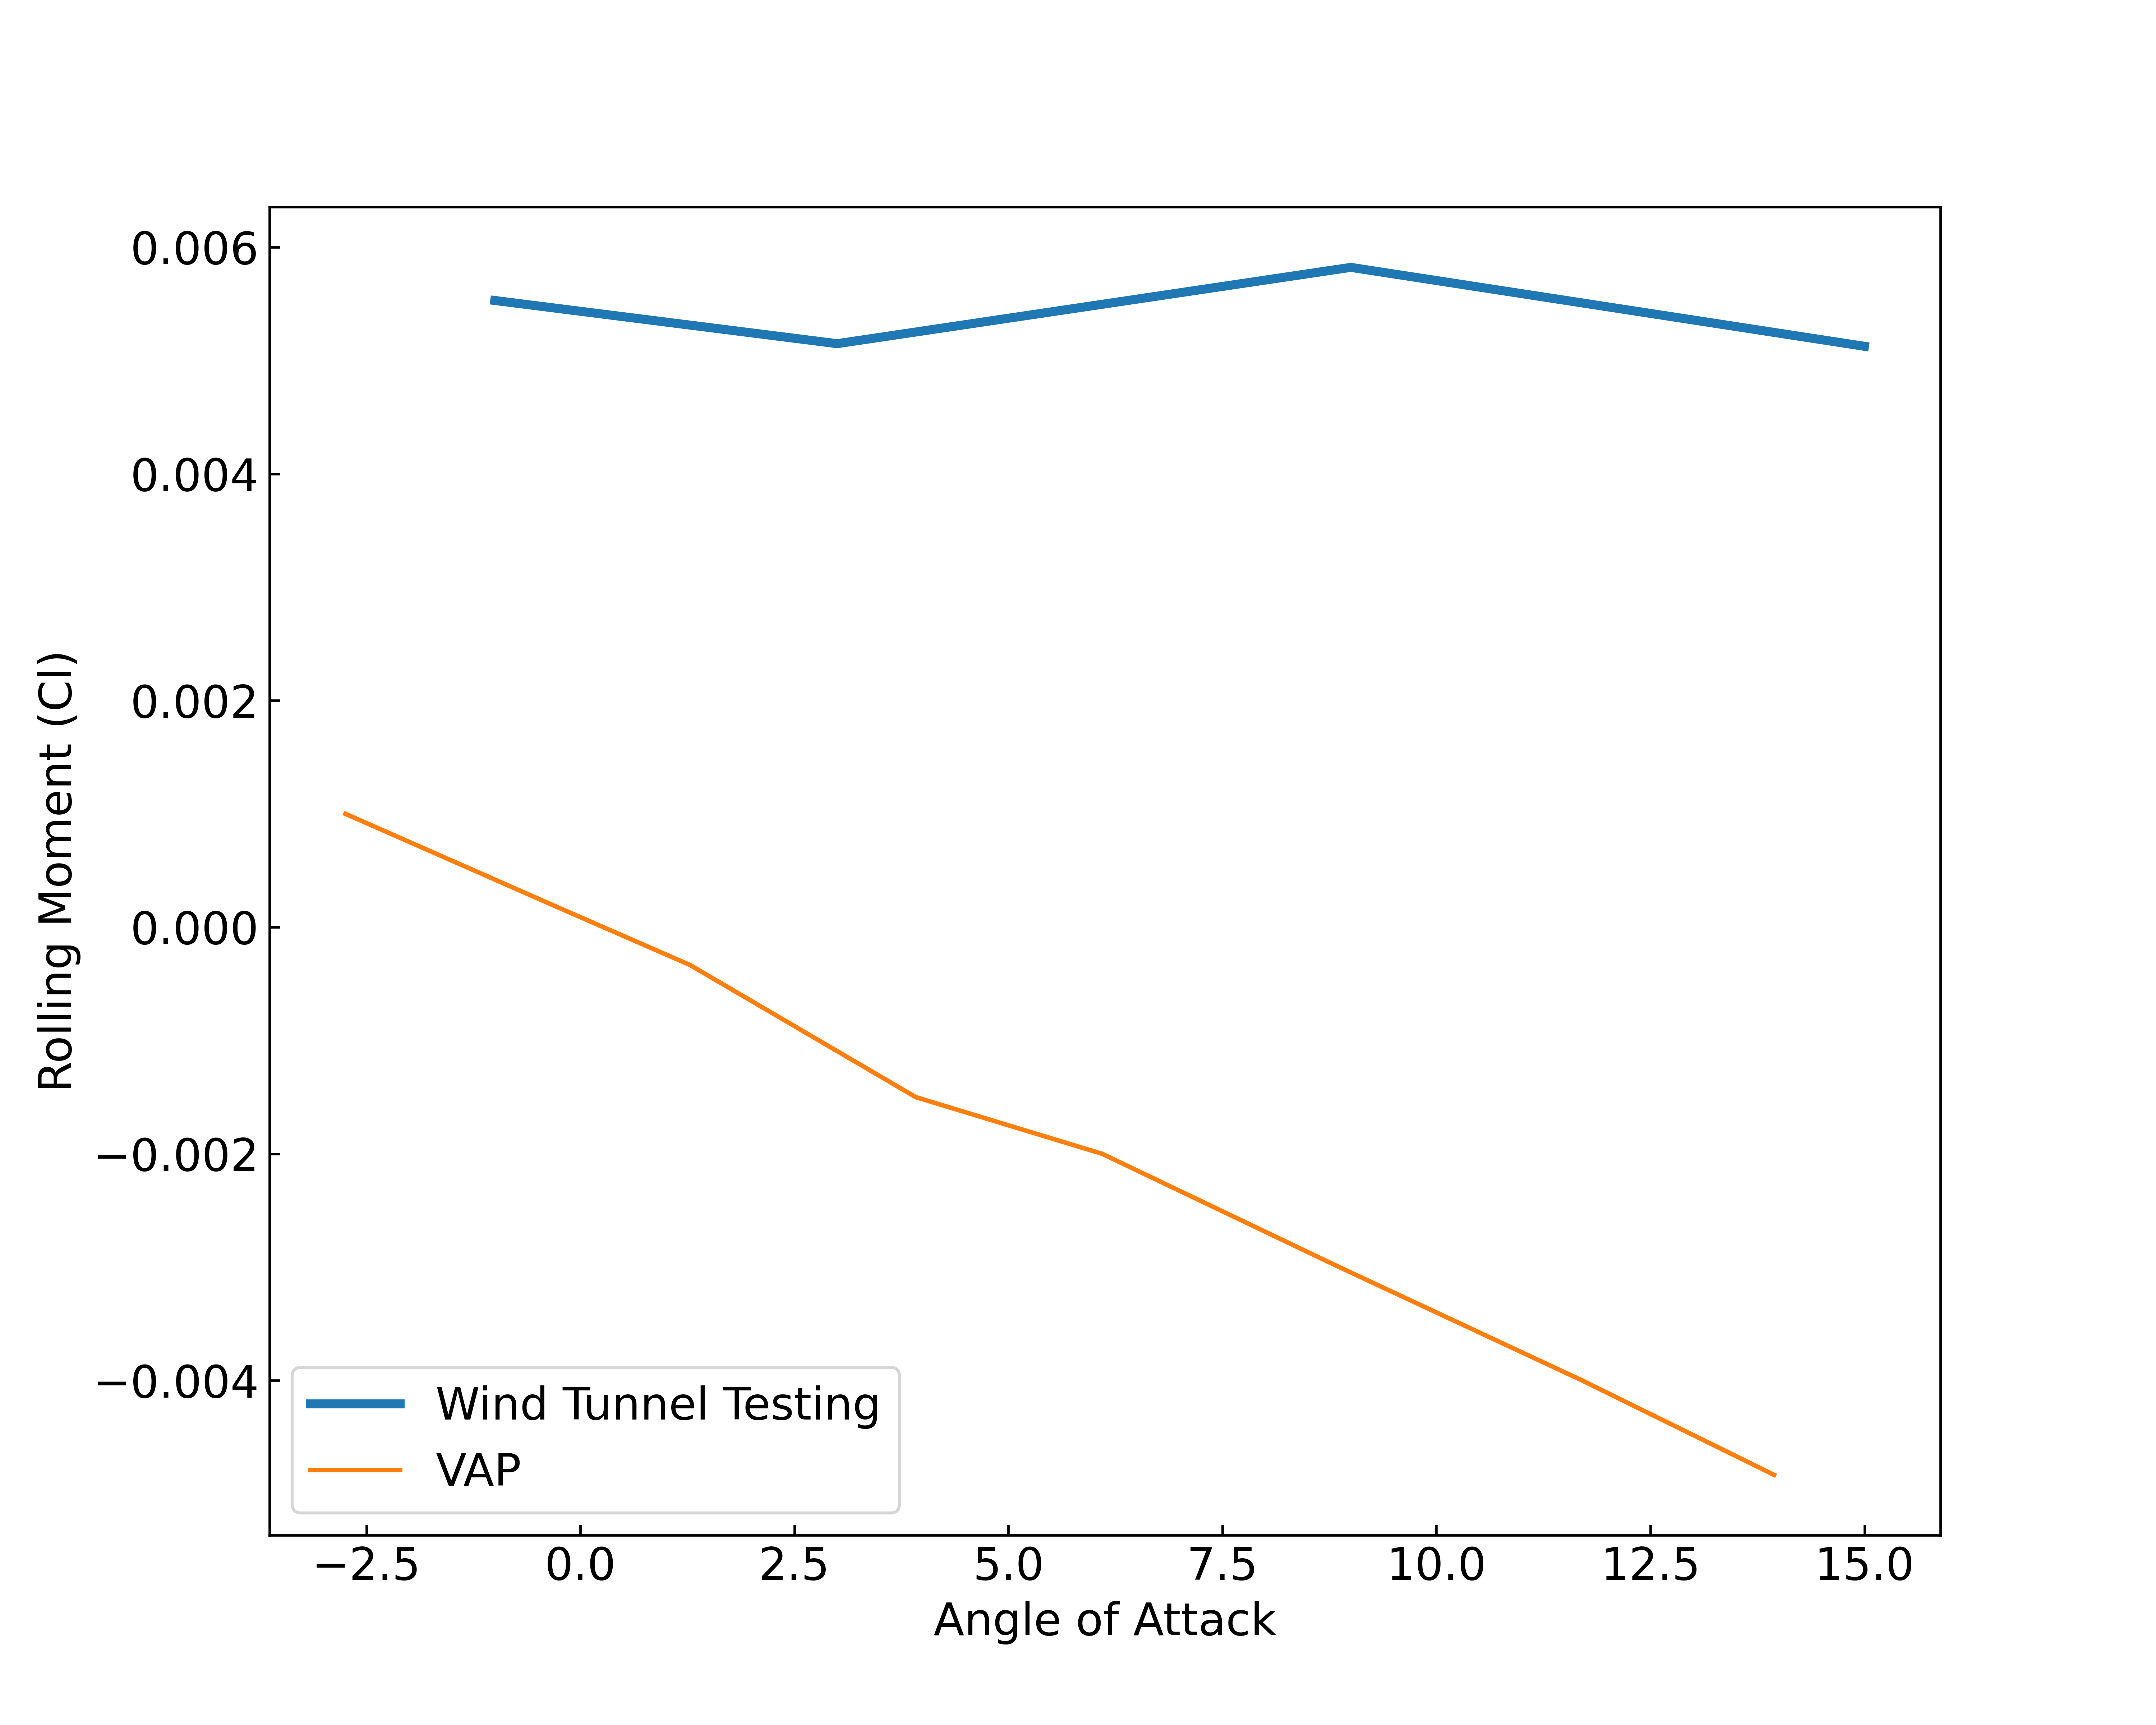
\includegraphics[width=\textwidth]{05_Results/VAP/noProp/Cl/10ms_11000RPM_Cl.png}
        \caption{Rolling Moment Coefficient at 10m/s airspeed and 11000RPM motor speed}
        \label{fig:VAP_NoProp_Cl_10ms_11000}
    \end{subfigure}
    \begin{subfigure}[b]{0.467\textwidth}
        \centering
        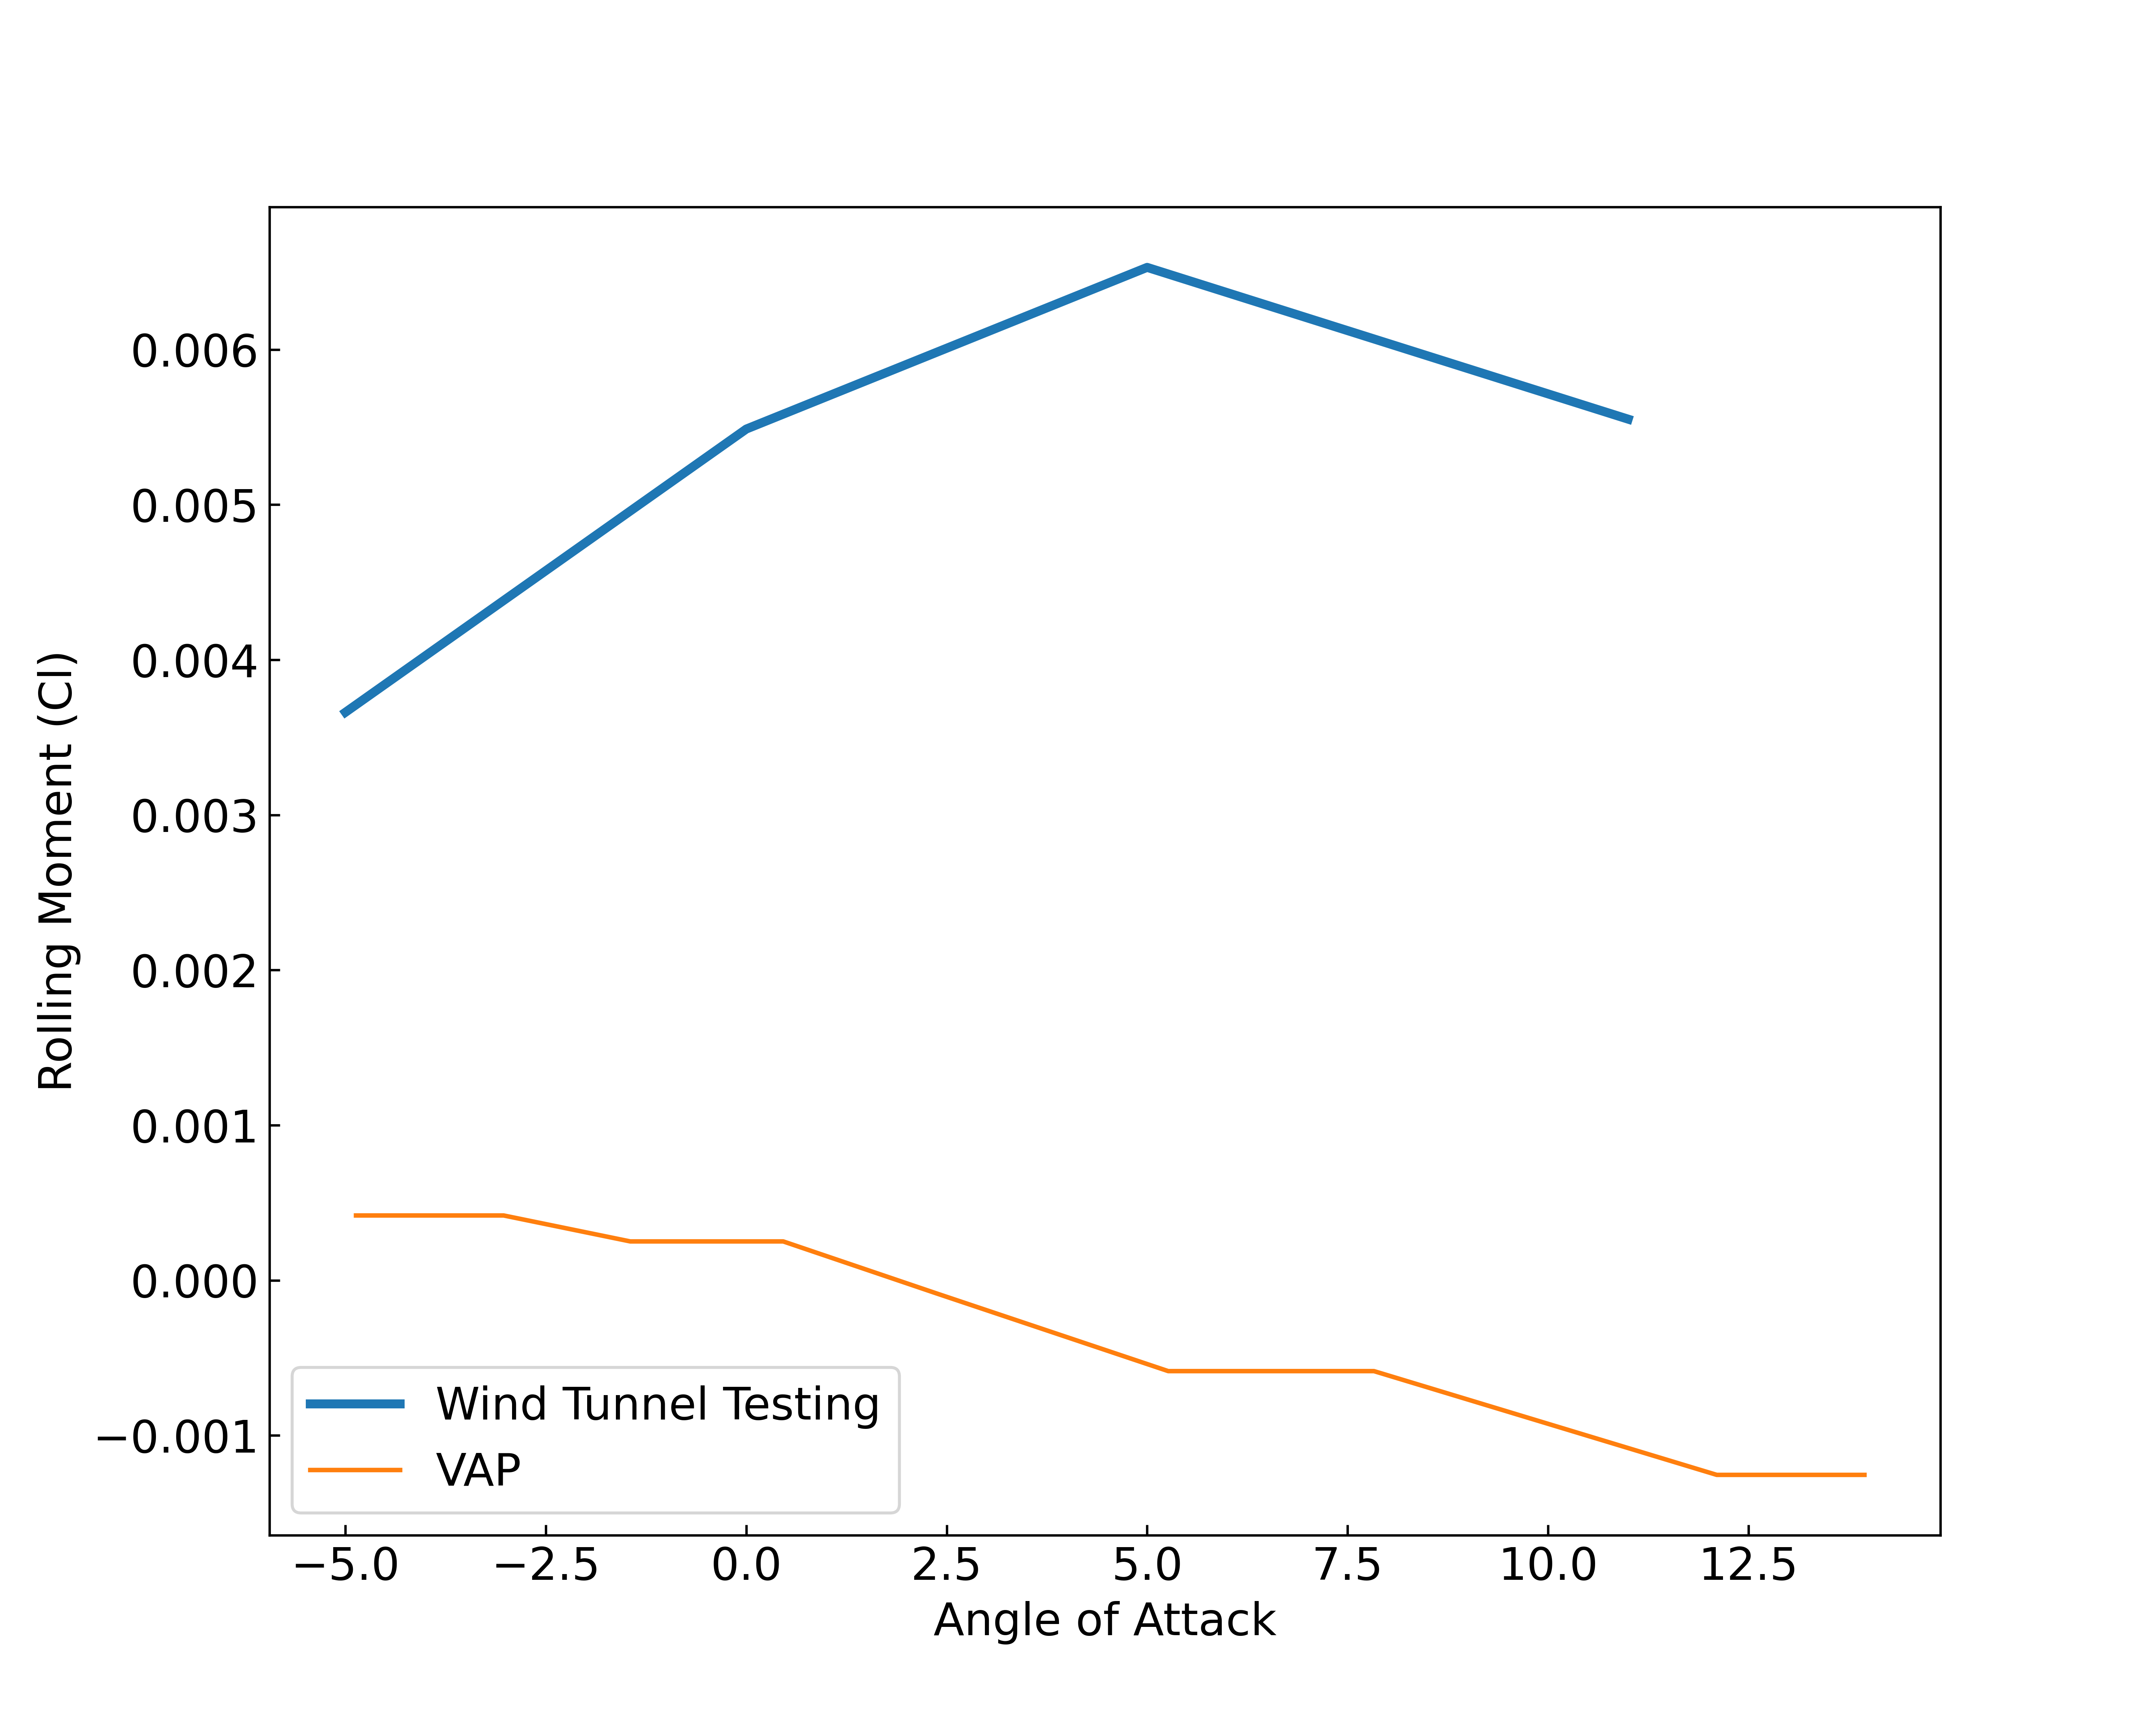
\includegraphics[width=\textwidth]{05_Results/VAP/noProp/Cl/20ms_6000RPM_Cl.png}
        \caption{Rolling Moment Coefficient at 20m/s airspeed and 6000RPM motor speed}
        \label{fig:VAP_NoProp_Cl_20ms_6000}
    \end{subfigure}
    \begin{subfigure}[b]{0.467\textwidth}
        \centering
        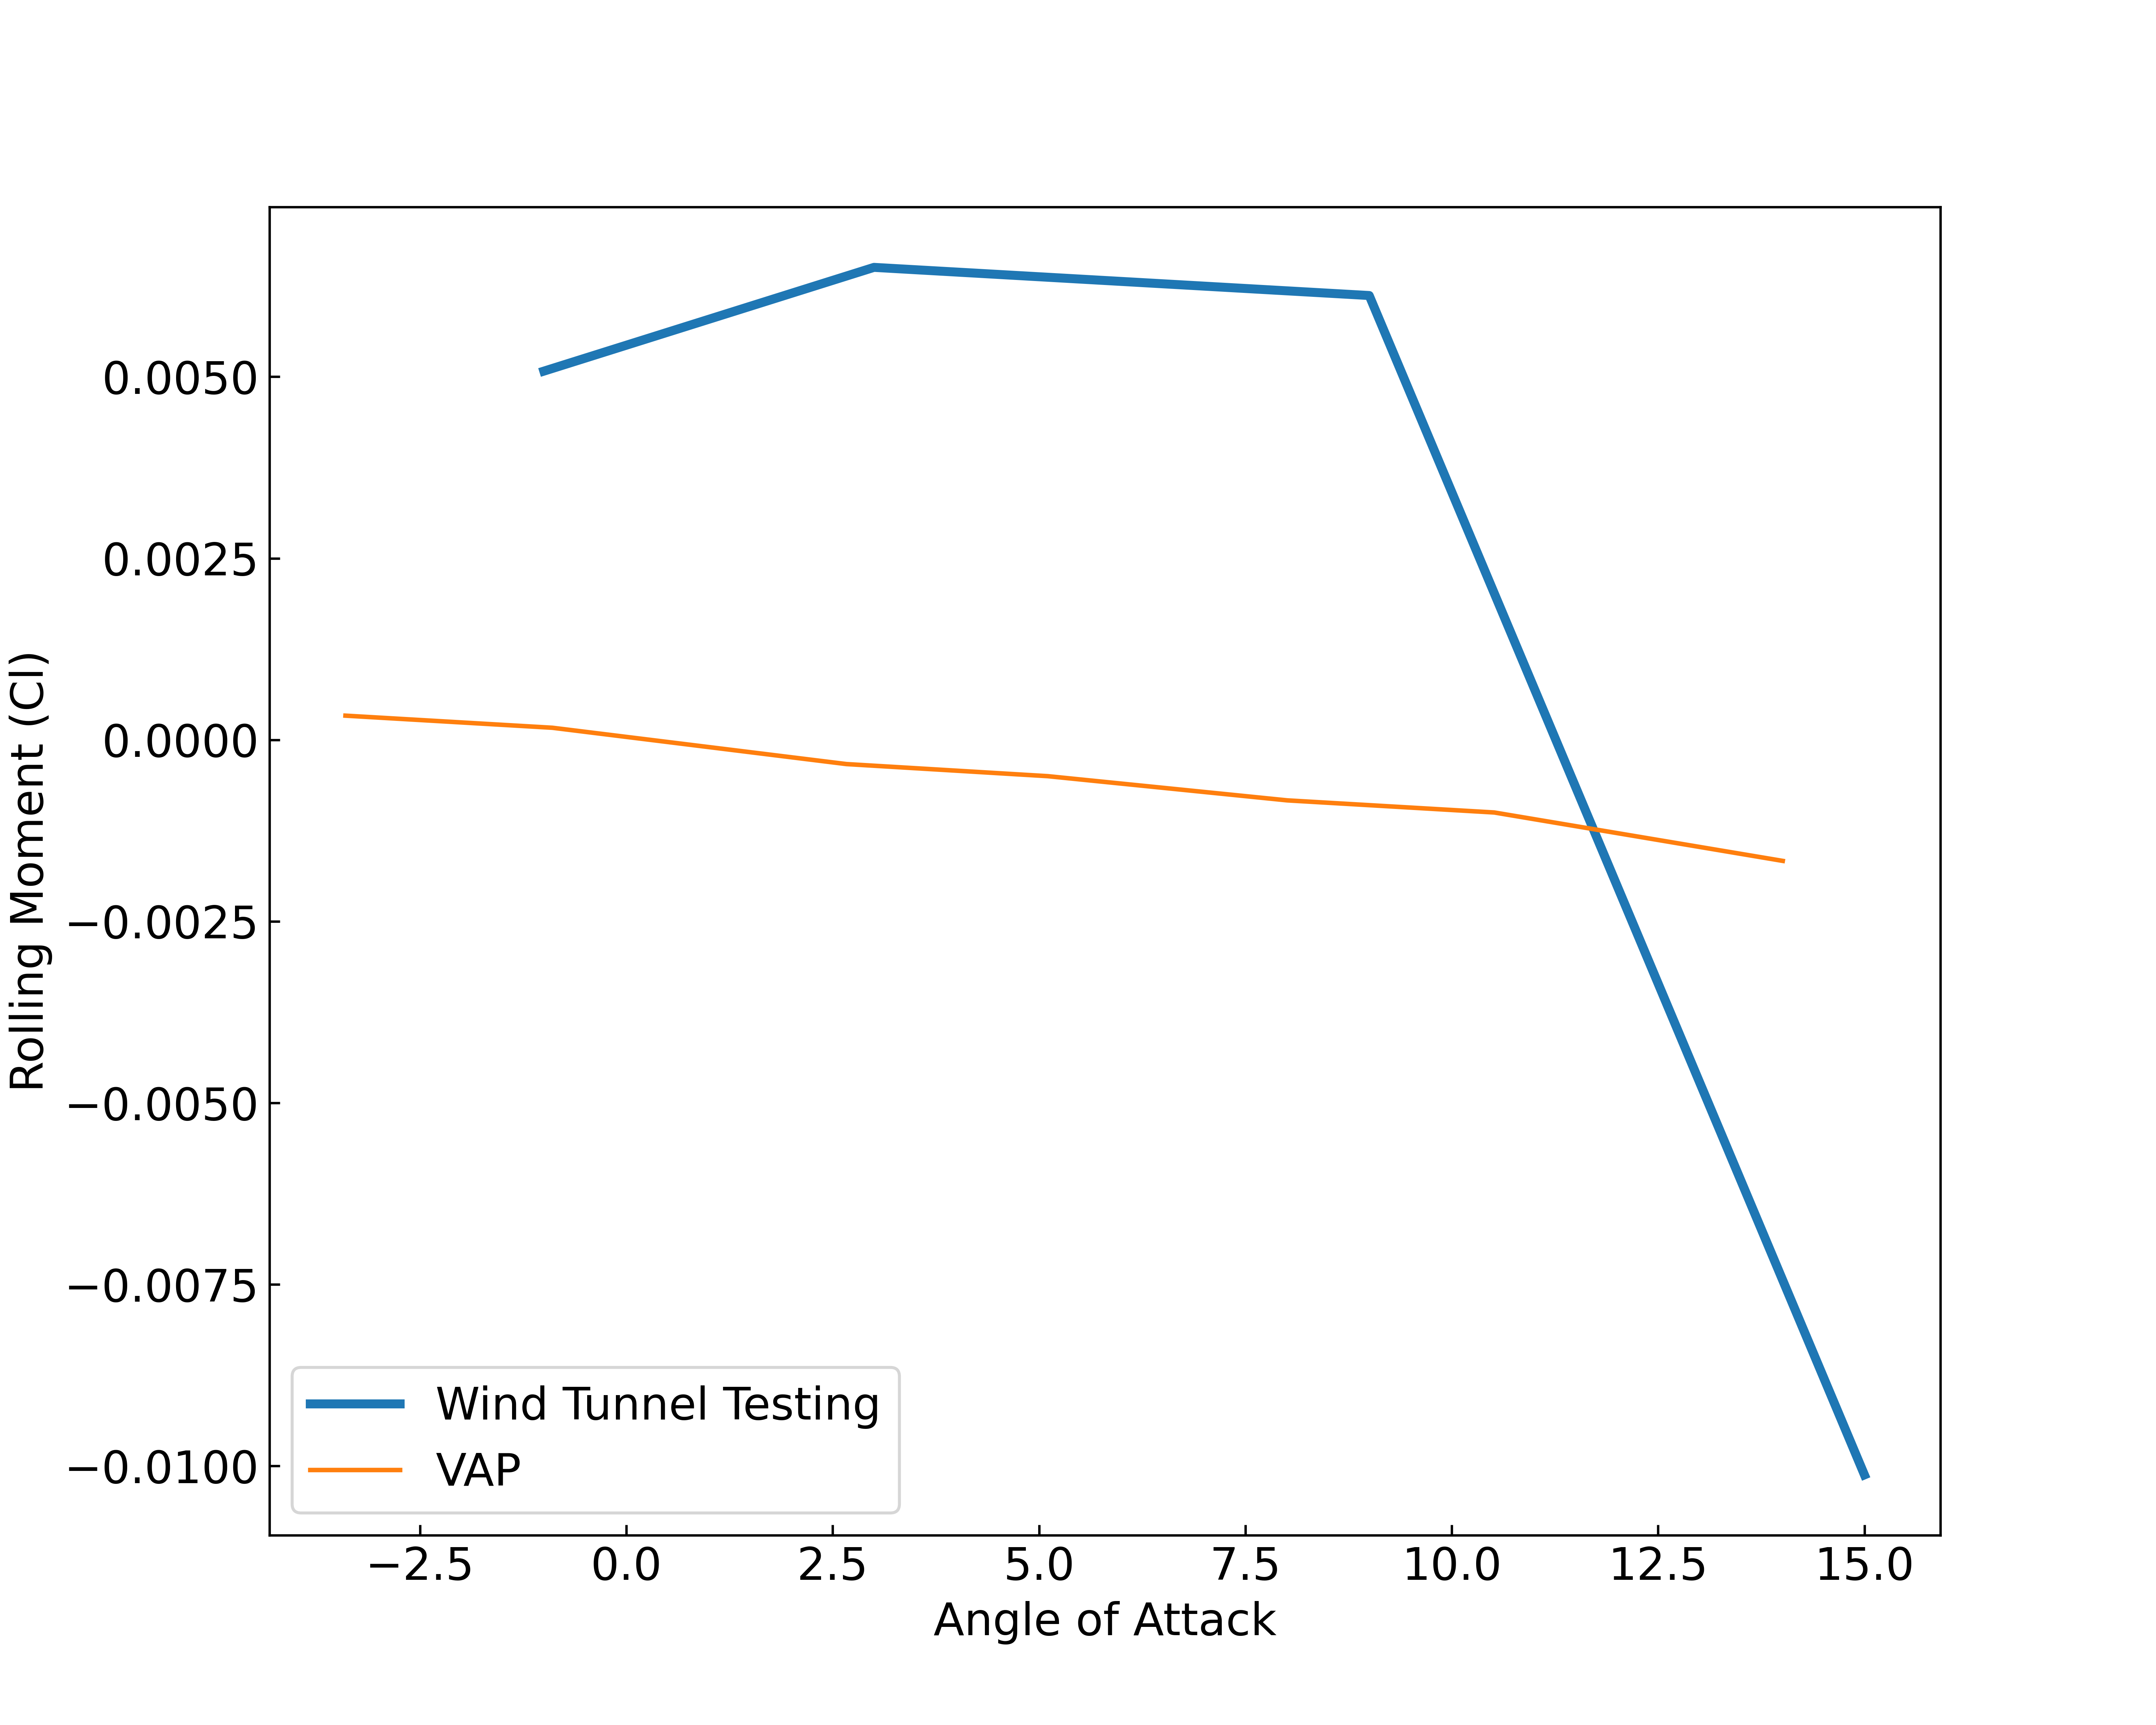
\includegraphics[width=\textwidth]{05_Results/VAP/noProp/Cl/20ms_11000RPM_Cl.png}
        \caption{Rolling Moment Coefficient at 20m/s airspeed and 11000RPM motor speed}
        \label{fig:VAP_NoProp_Cl_20ms_11000}
    \end{subfigure}
\end{figure}


\begin{figure}[H]
    \centering
    \begin{subfigure}[b]{0.467\textwidth}
        \centering
        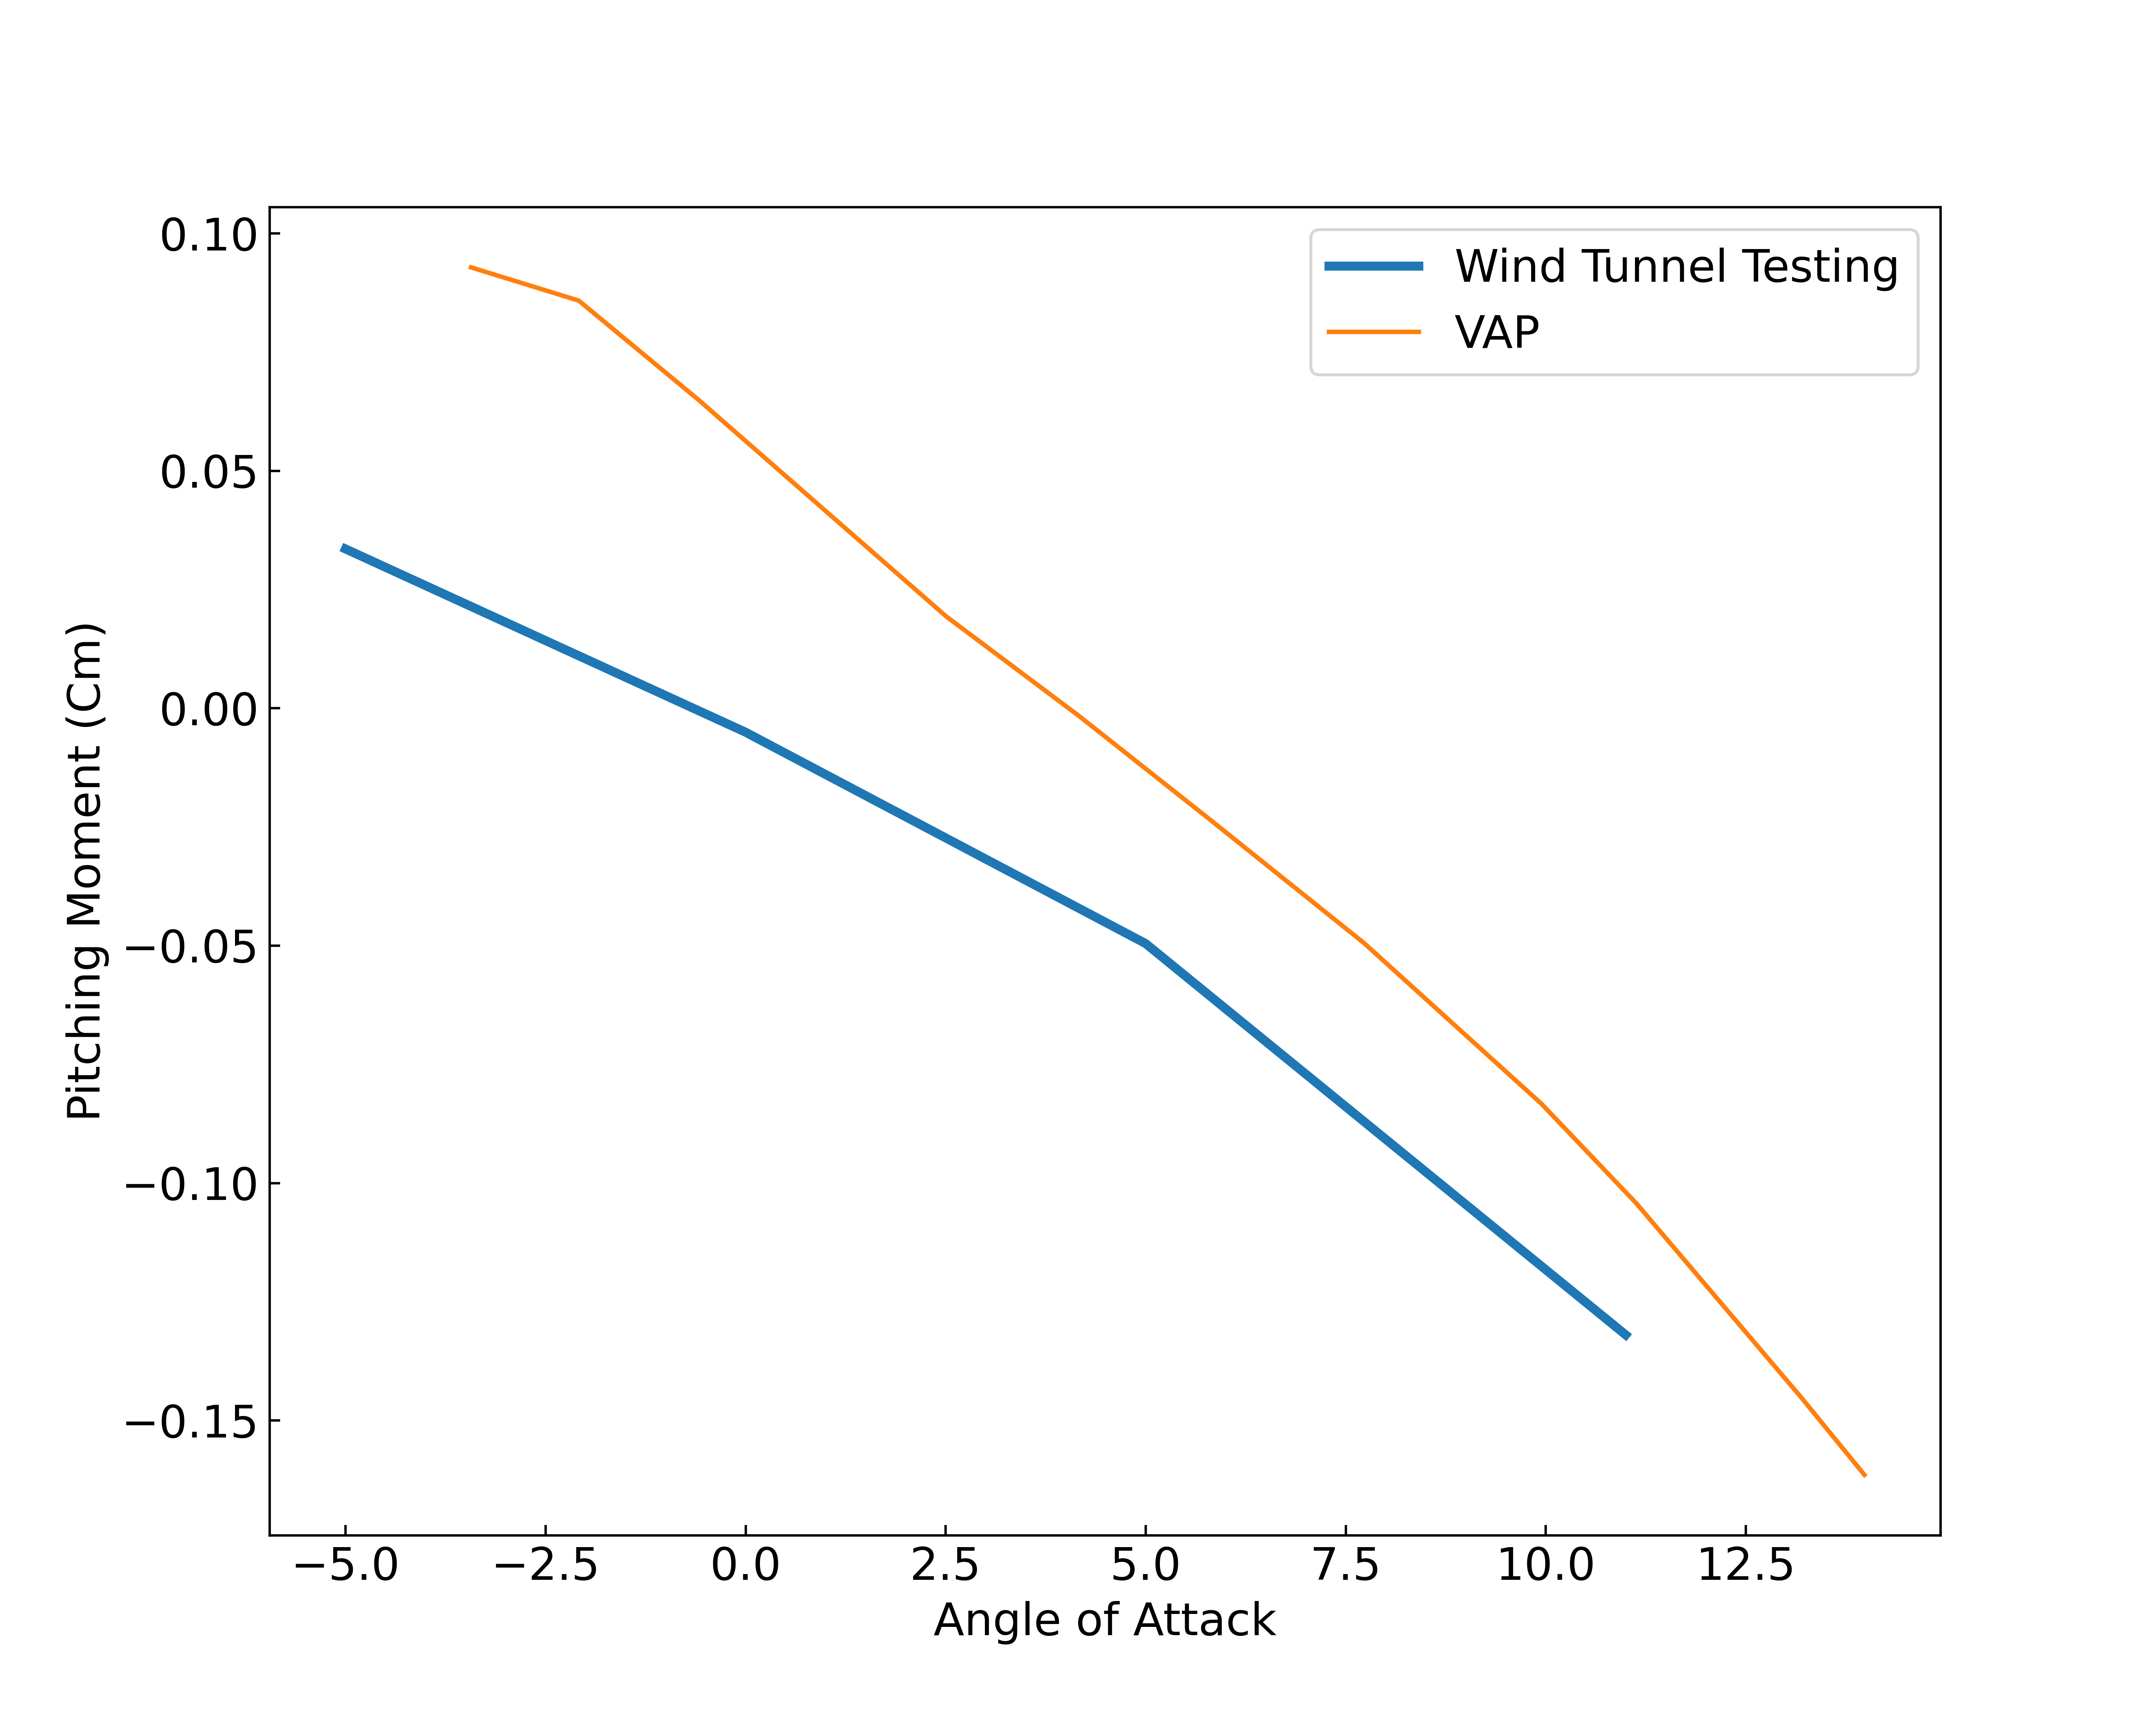
\includegraphics[width=\textwidth]{05_Results/VAP/noProp/Cm/10ms_6000RPM_Cm.png}
        \caption{Pitching Moment Coefficient at 10m/s airspeed and 6000RPM motor speed}
        \label{fig:VAP_NoProp_Cm_10ms_6000}
    \end{subfigure}
    \begin{subfigure}[b]{0.467\textwidth}
        \centering
        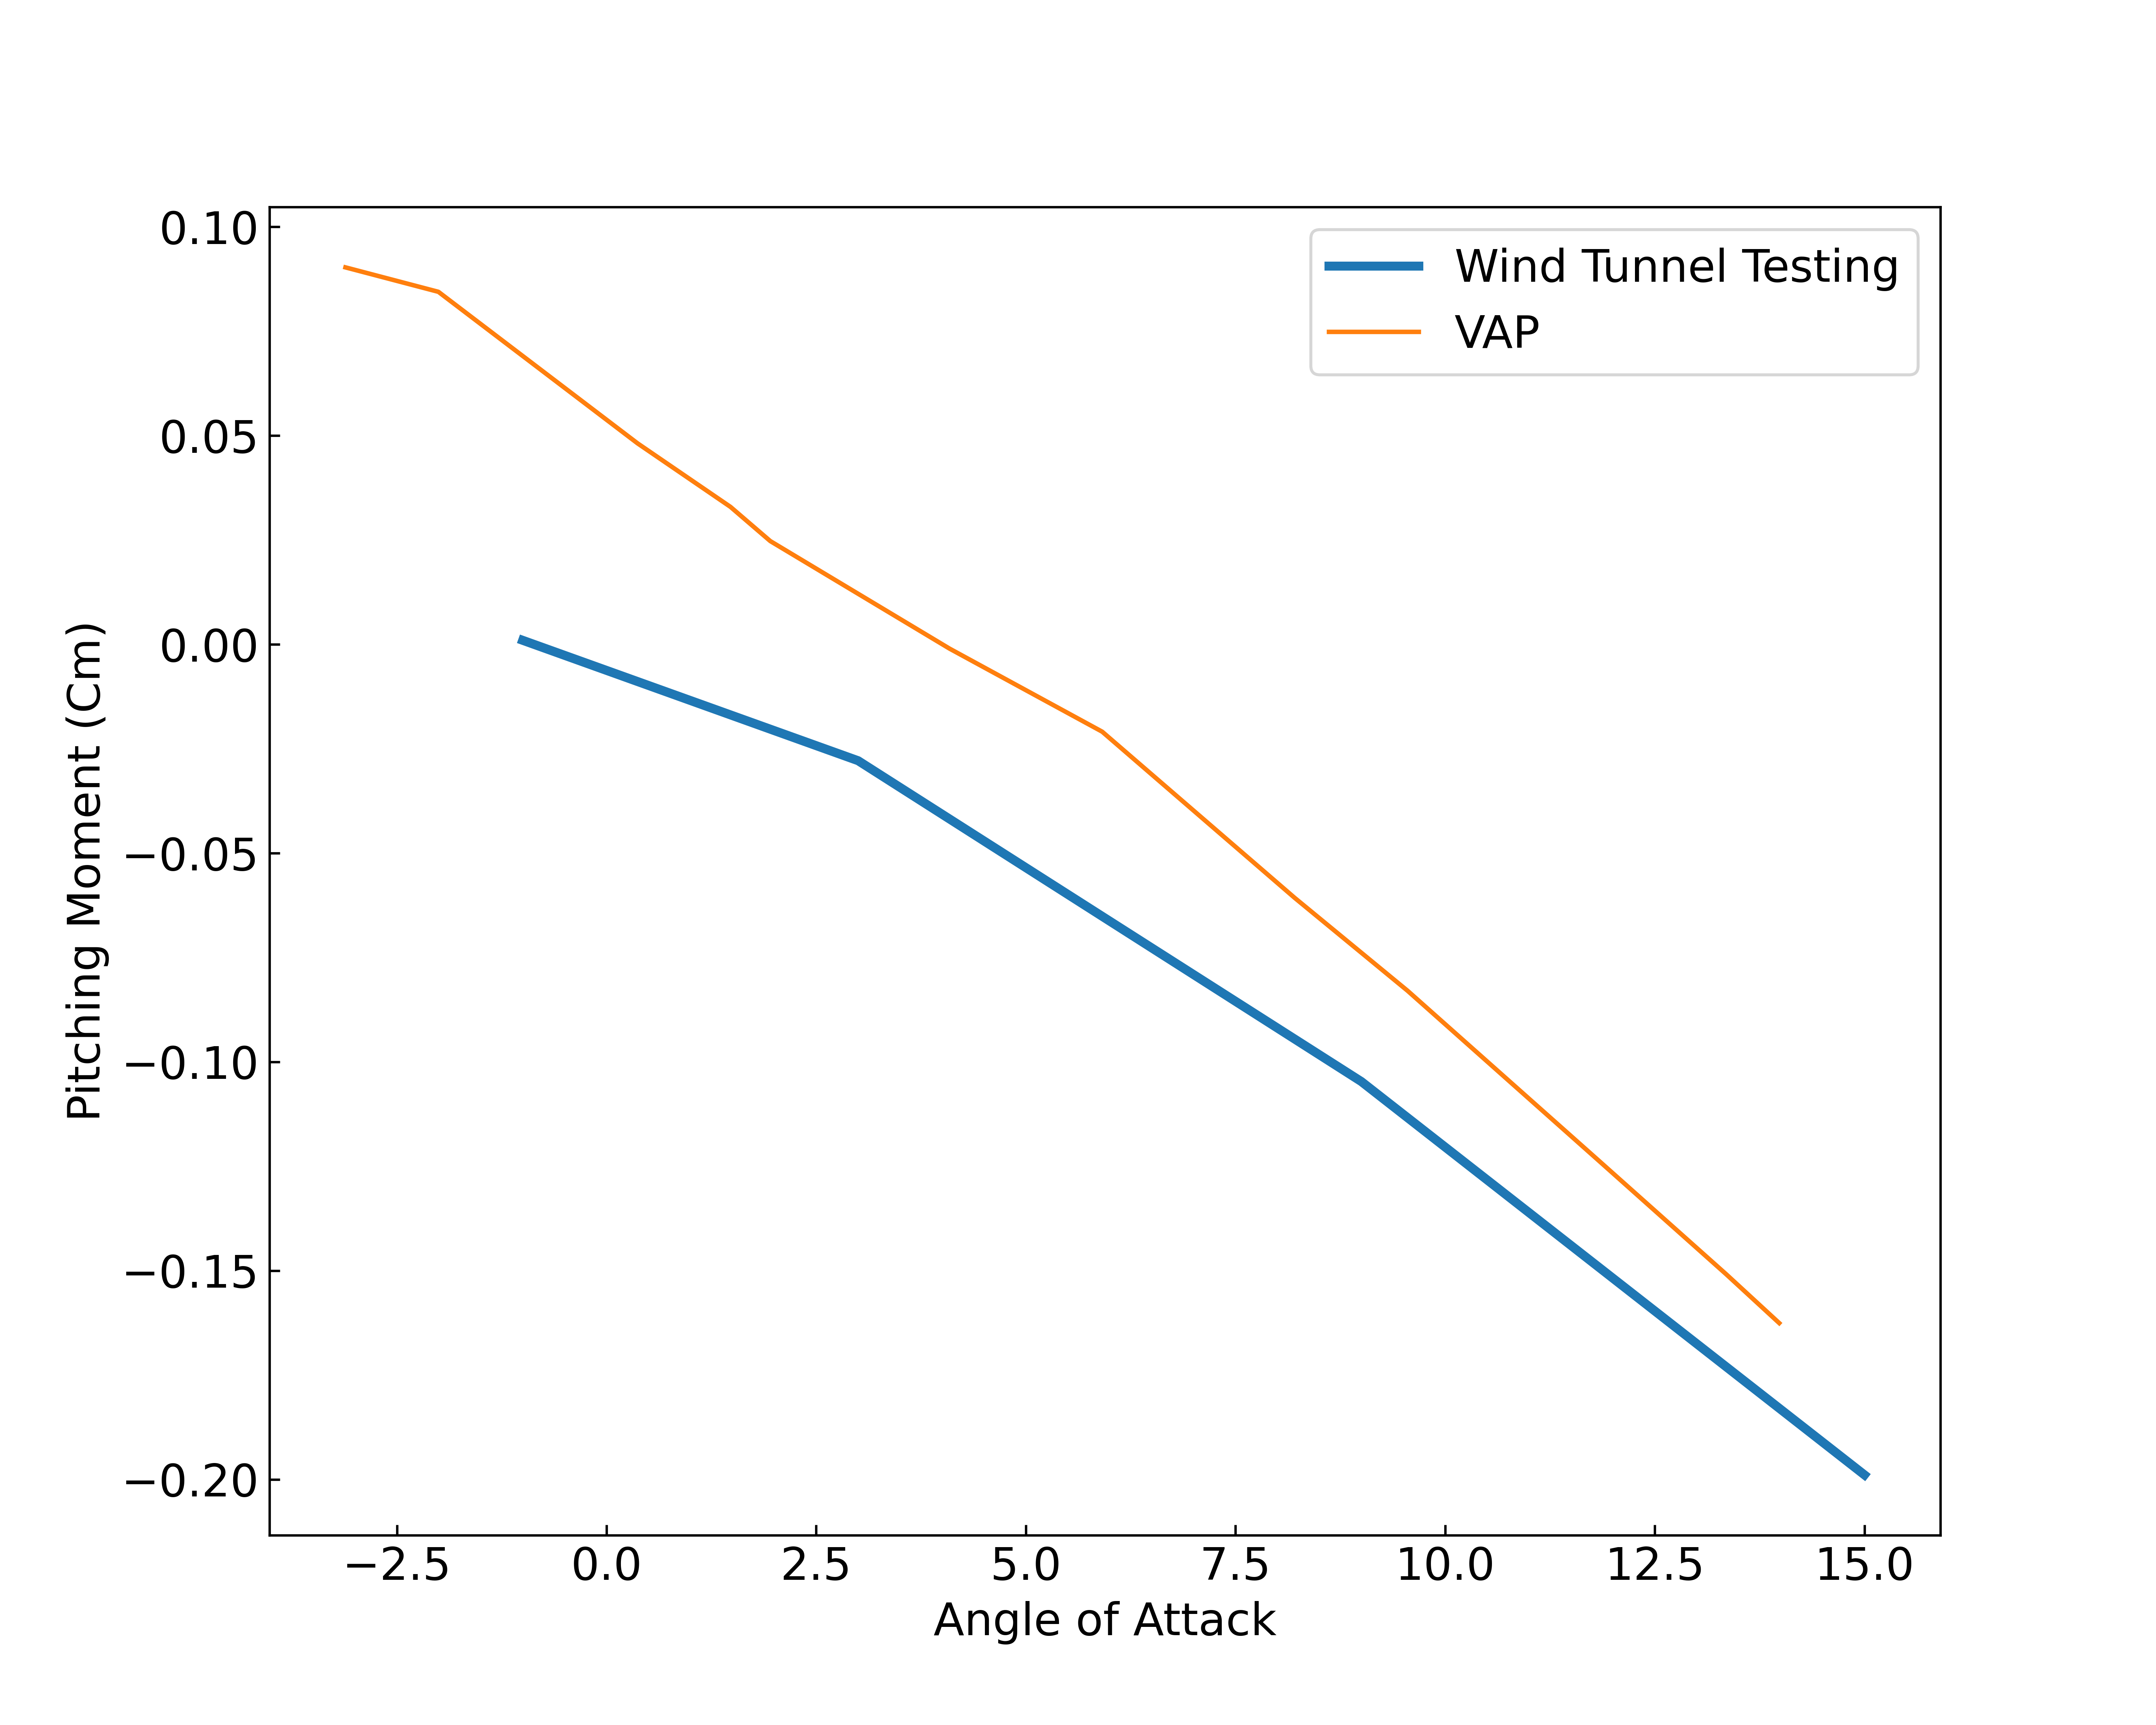
\includegraphics[width=\textwidth]{05_Results/VAP/noProp/Cm/10ms_11000RPM_Cm.png}
        \caption{Pitching Moment Coefficient at 10m/s airspeed and 11000RPM motor speed}
        \label{fig:VAP_NoProp_Cm_10ms_11000}
    \end{subfigure}
    \begin{subfigure}[b]{0.467\textwidth}
        \centering
        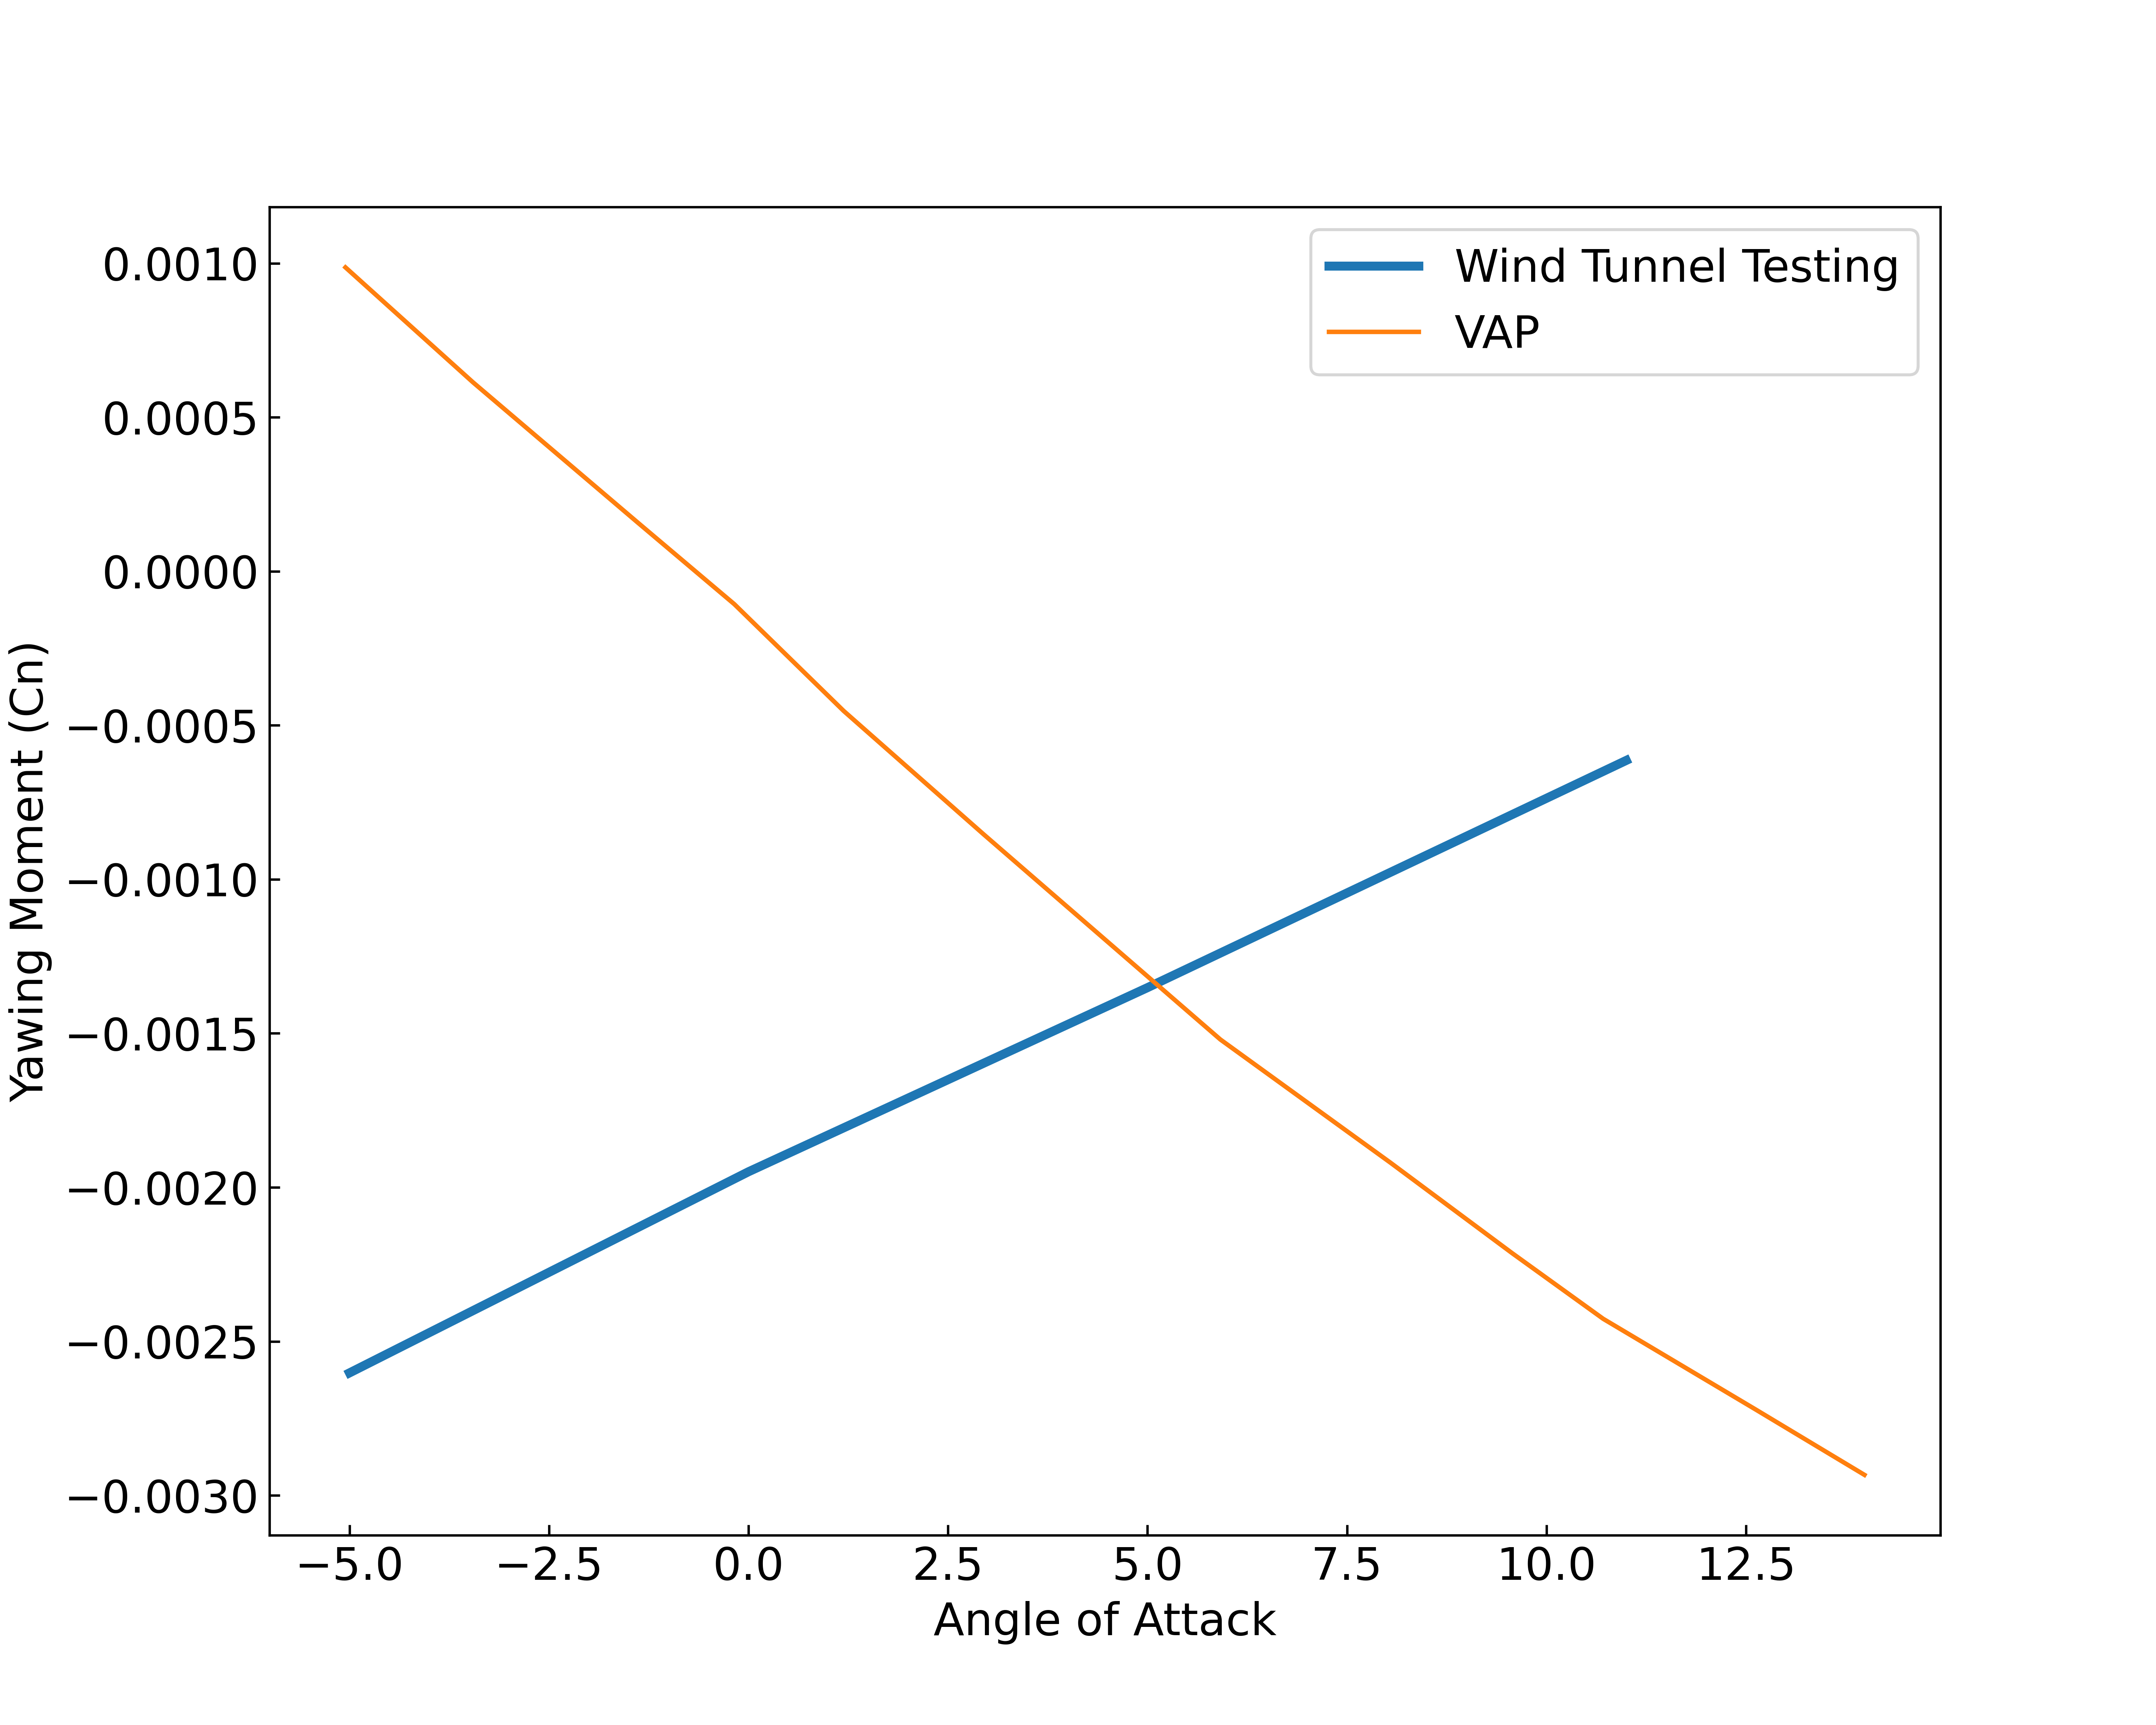
\includegraphics[width=\textwidth]{05_Results/VAP/noProp/Cn/20ms_6000RPM_Cn.png}
        \caption{Pitching Moment Coefficient at 20m/s airspeed and 6000RPM motor speed}
        \label{fig:VAP_NoProp_Cm_20ms_6000}
    \end{subfigure}
    \begin{subfigure}[b]{0.467\textwidth}
        \centering
        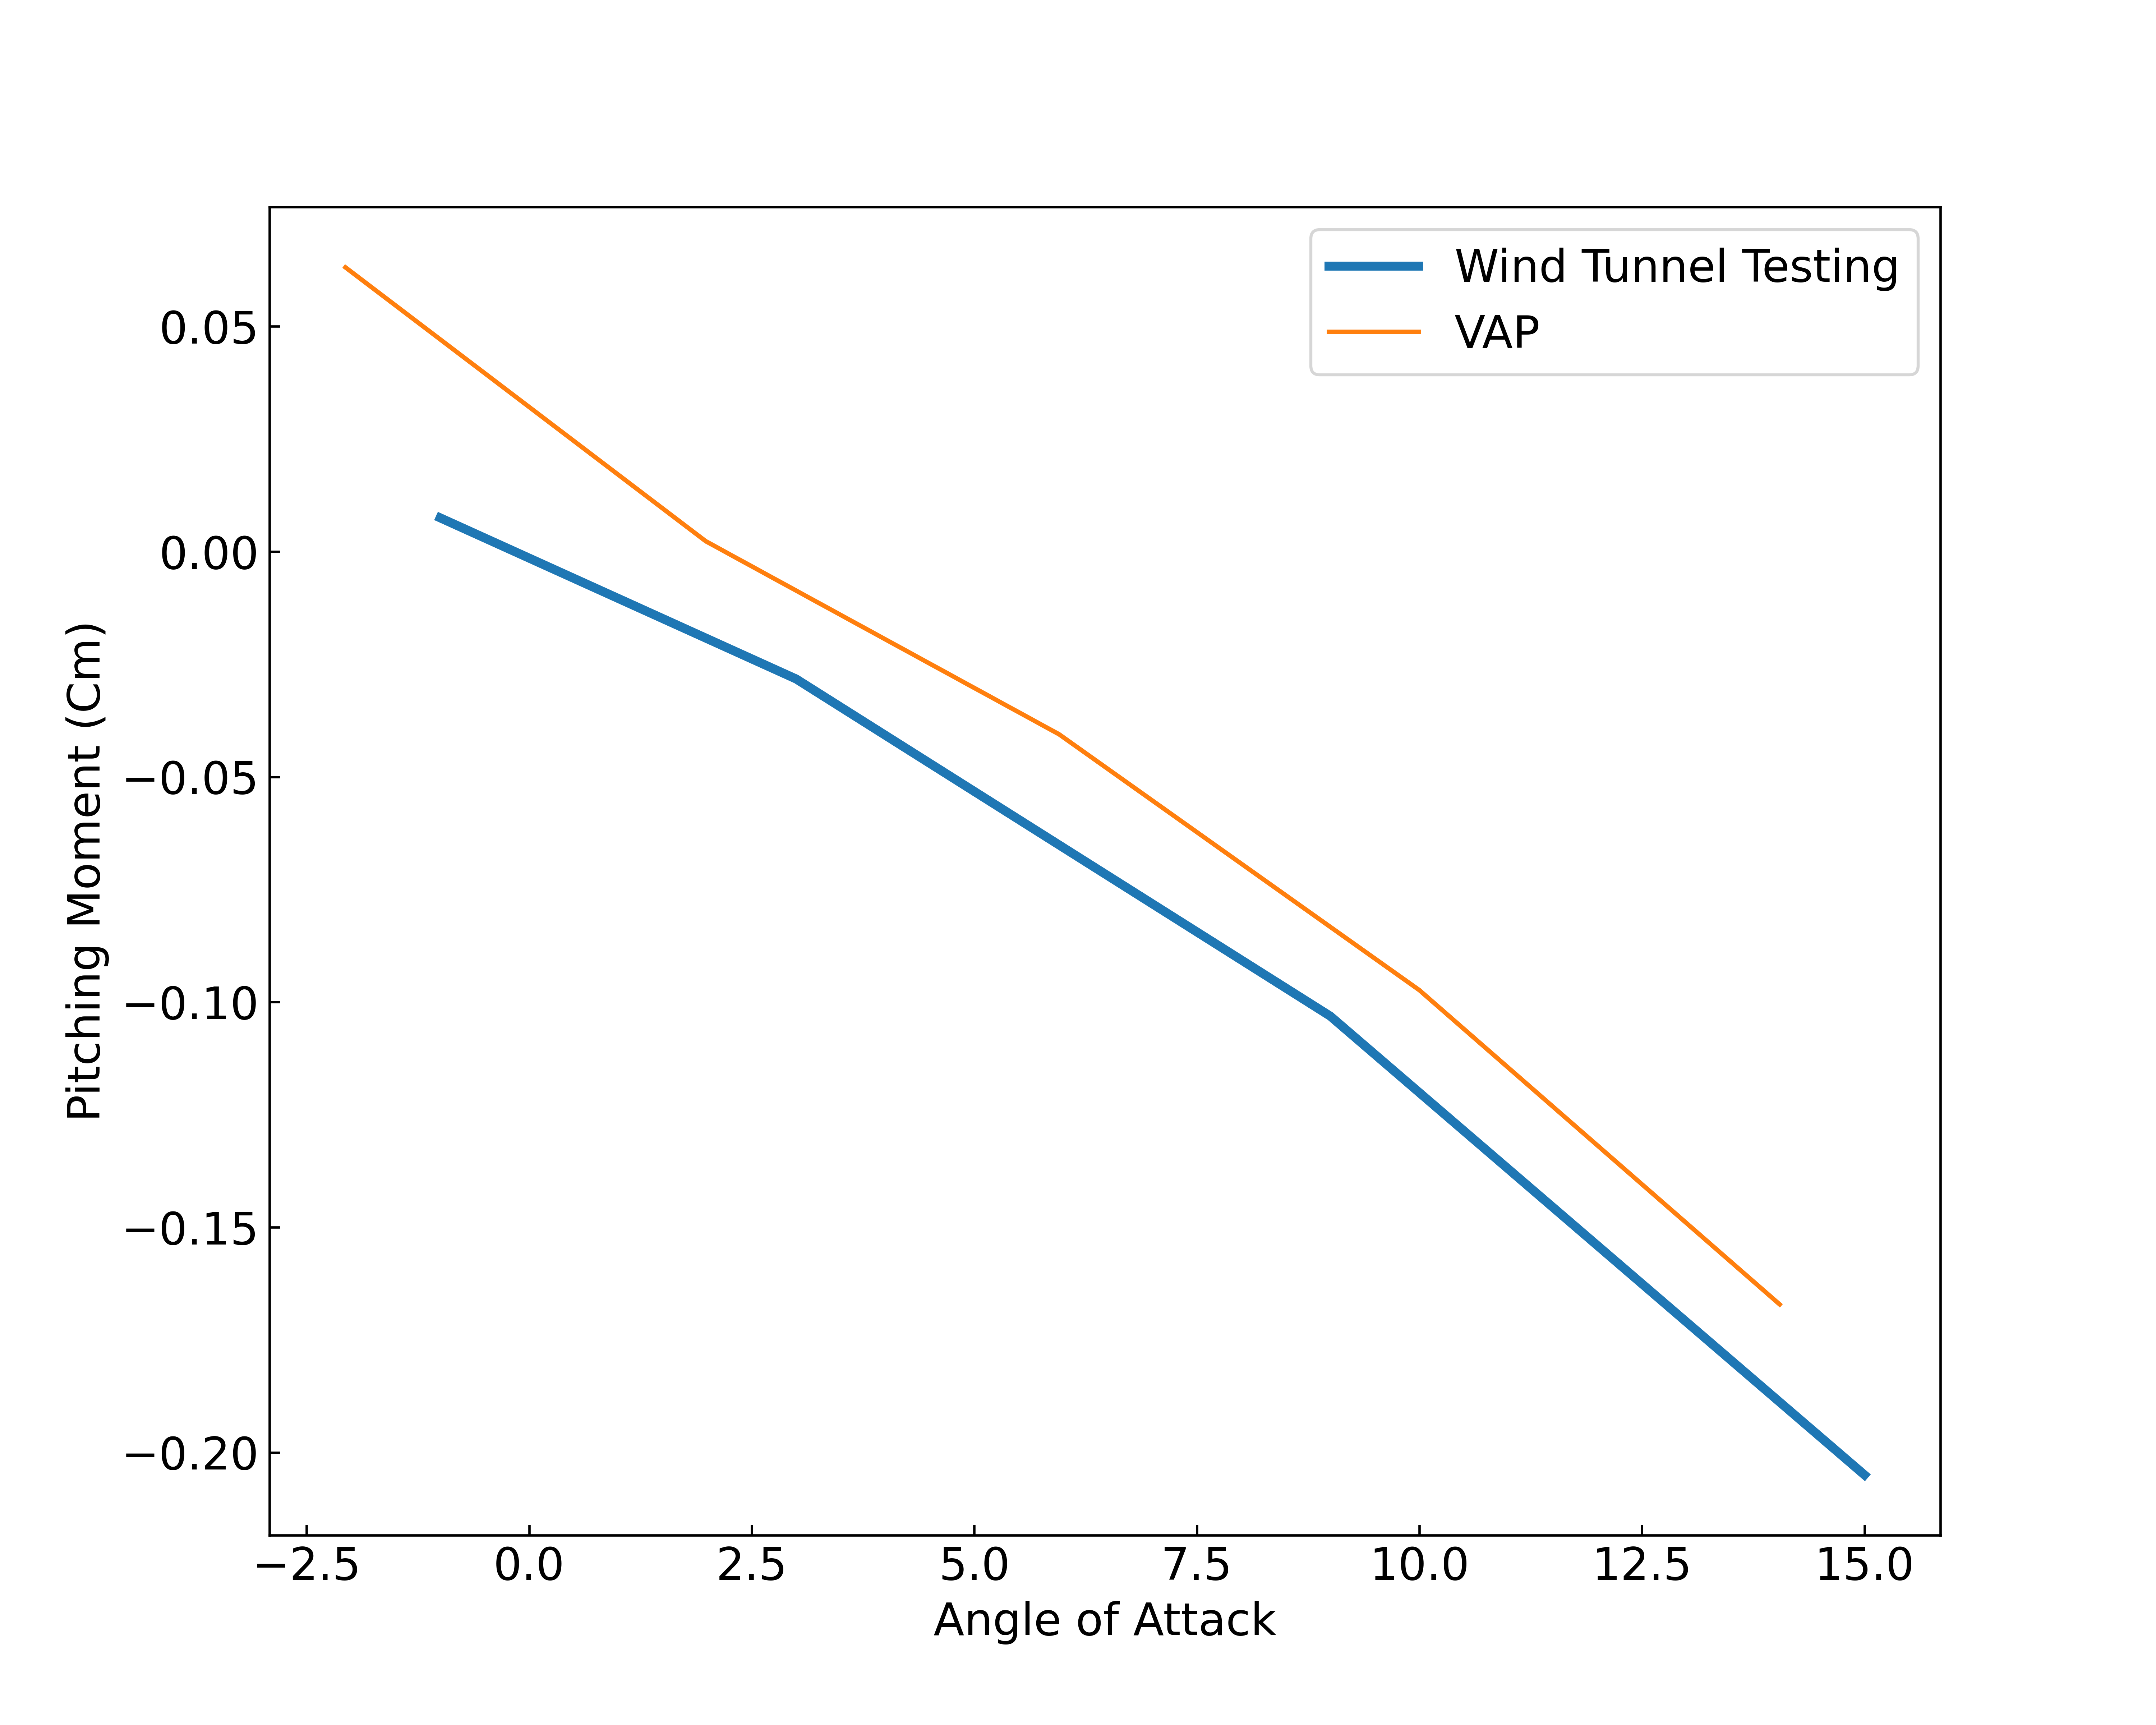
\includegraphics[width=\textwidth]{05_Results/VAP/noProp/Cm/20ms_11000RPM_Cm.png}
        \caption{Pitching Moment Coefficient at 20m/s airspeed and 11000RPM motor speed}
        \label{fig:VAP_NoProp_Cm_20ms_11000}
    \end{subfigure}
\end{figure}



\begin{figure}[H]
    \centering
    \begin{subfigure}[b]{0.467\textwidth}
        \centering
        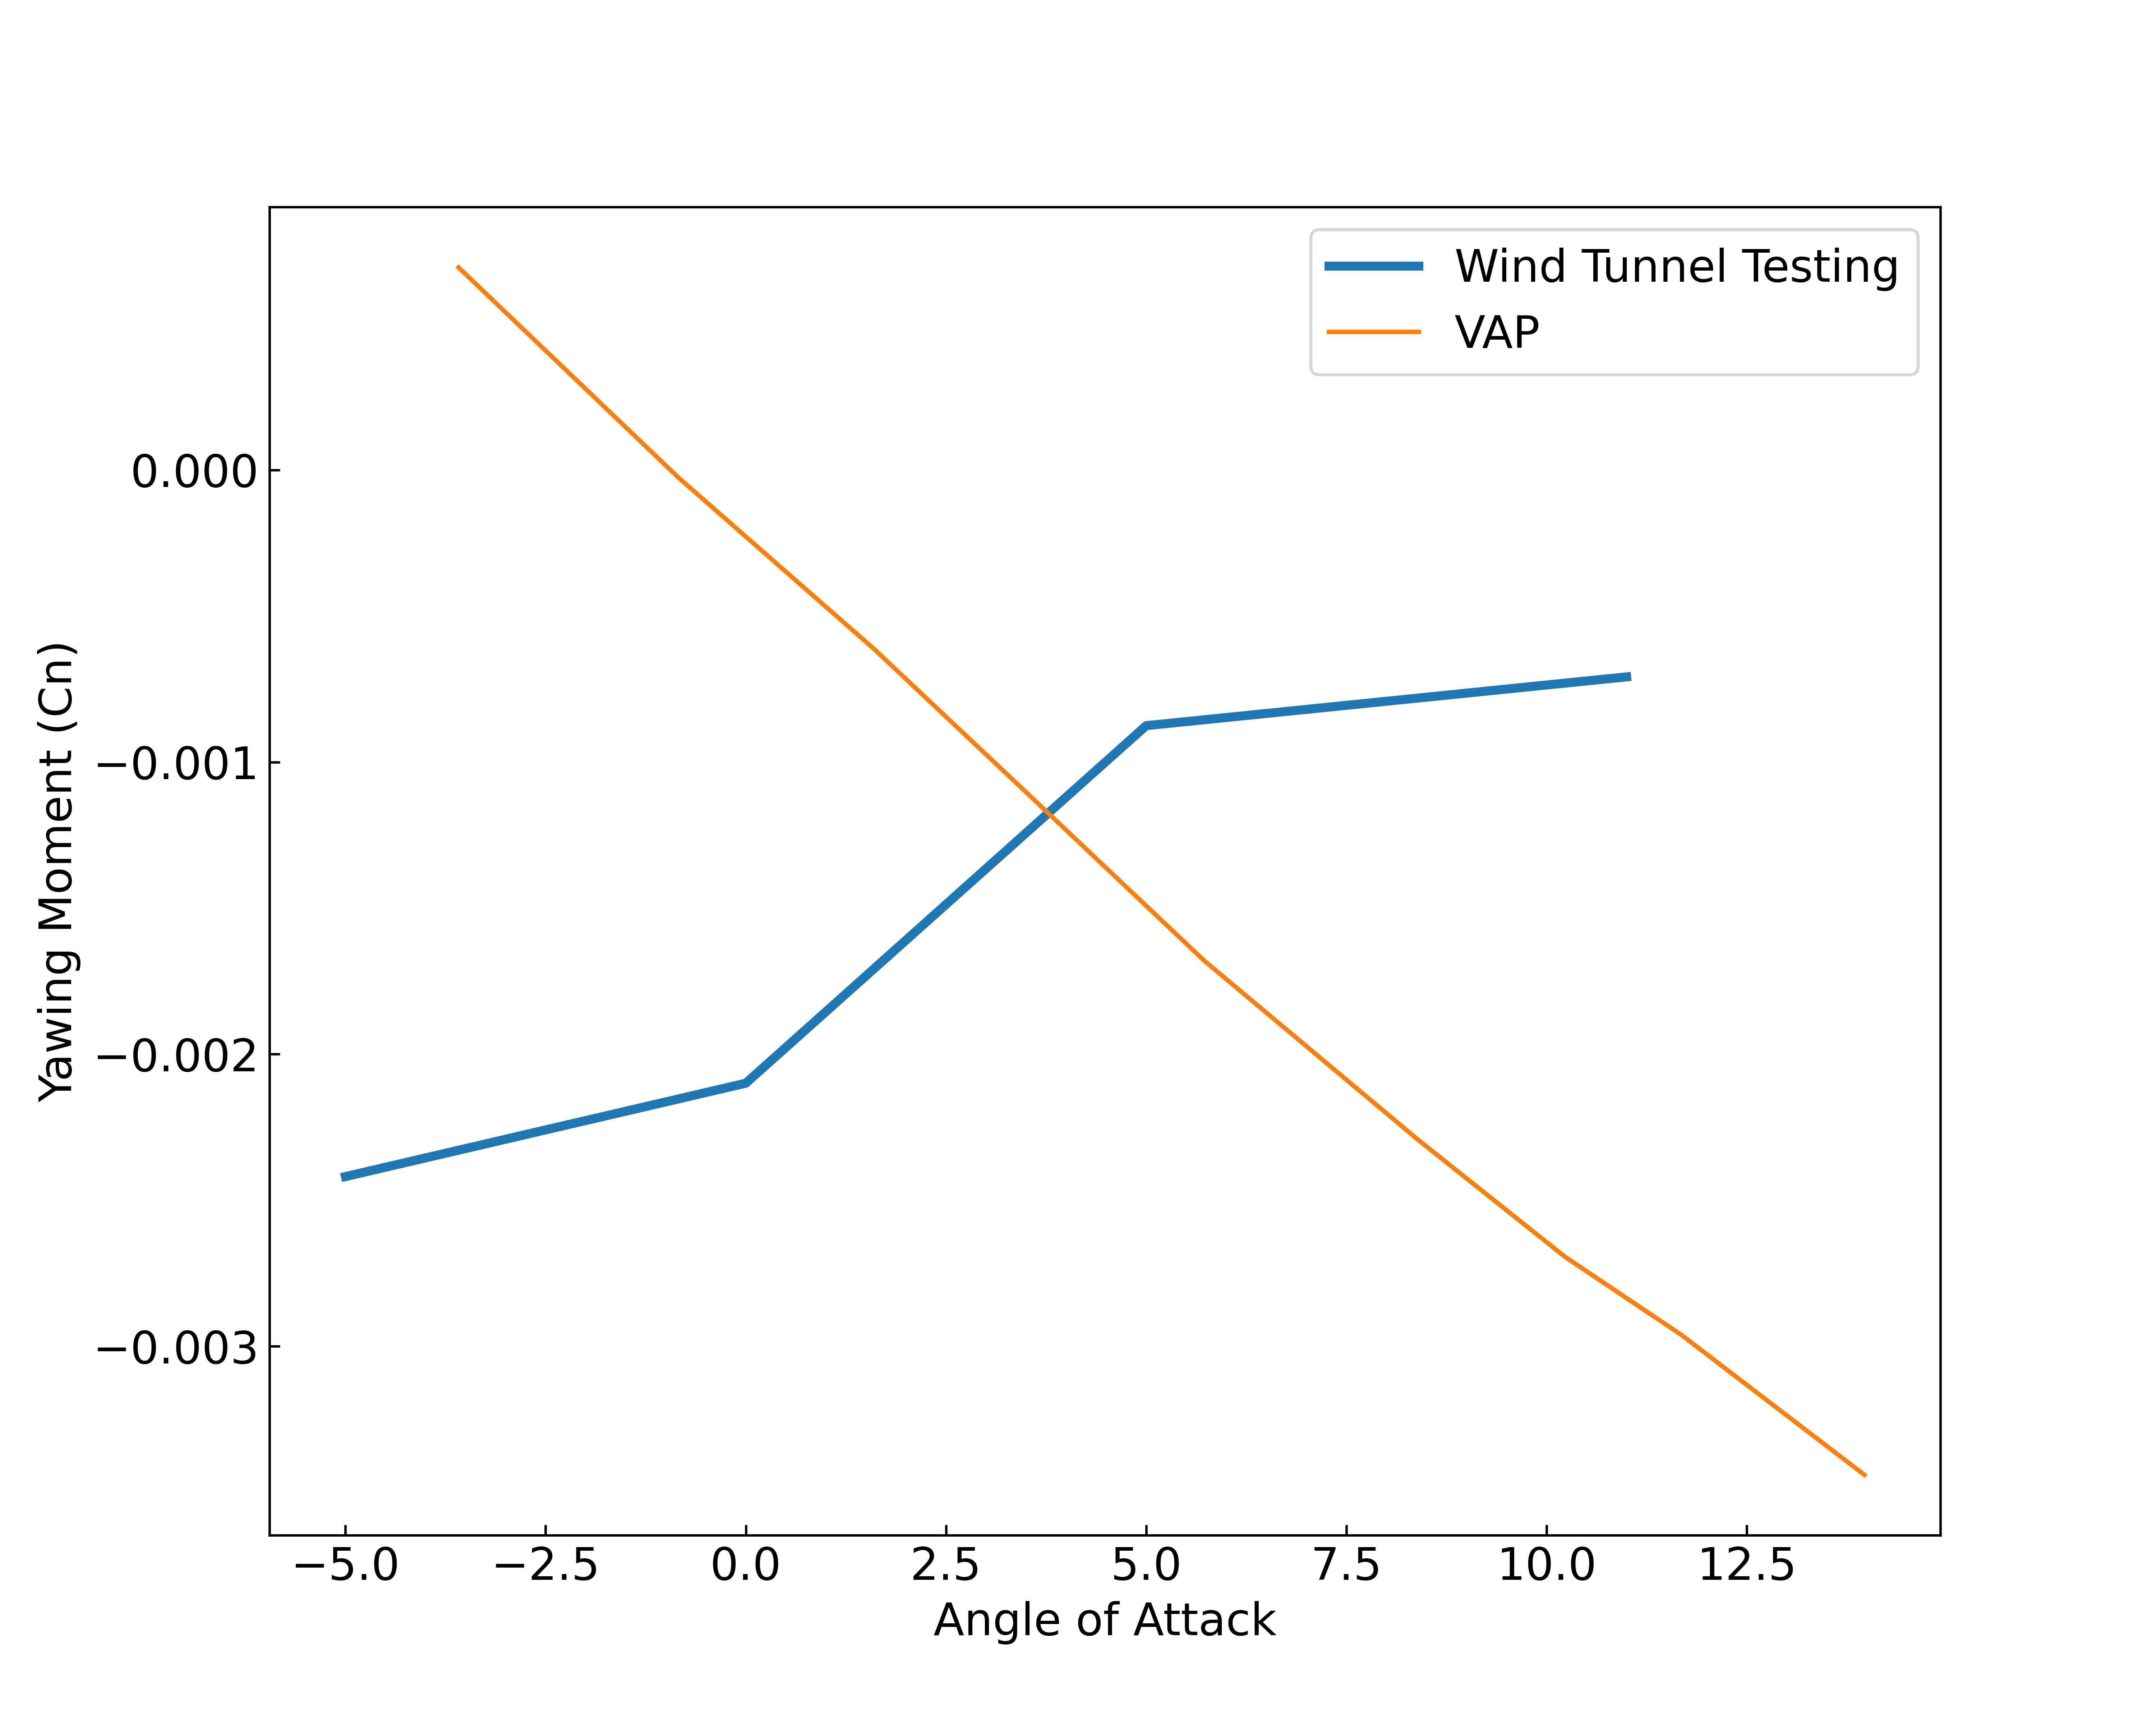
\includegraphics[width=\textwidth]{05_Results/VAP/noProp/Cn/10ms_6000RPM_Cn.png}
        \caption{Yawing Moment Coefficient at 10m/s airspeed and 6000RPM motor speed}
        \label{fig:VAP_noProp_Cm_10ms_6000}
    \end{subfigure}
    \begin{subfigure}[b]{0.467\textwidth}
        \centering
        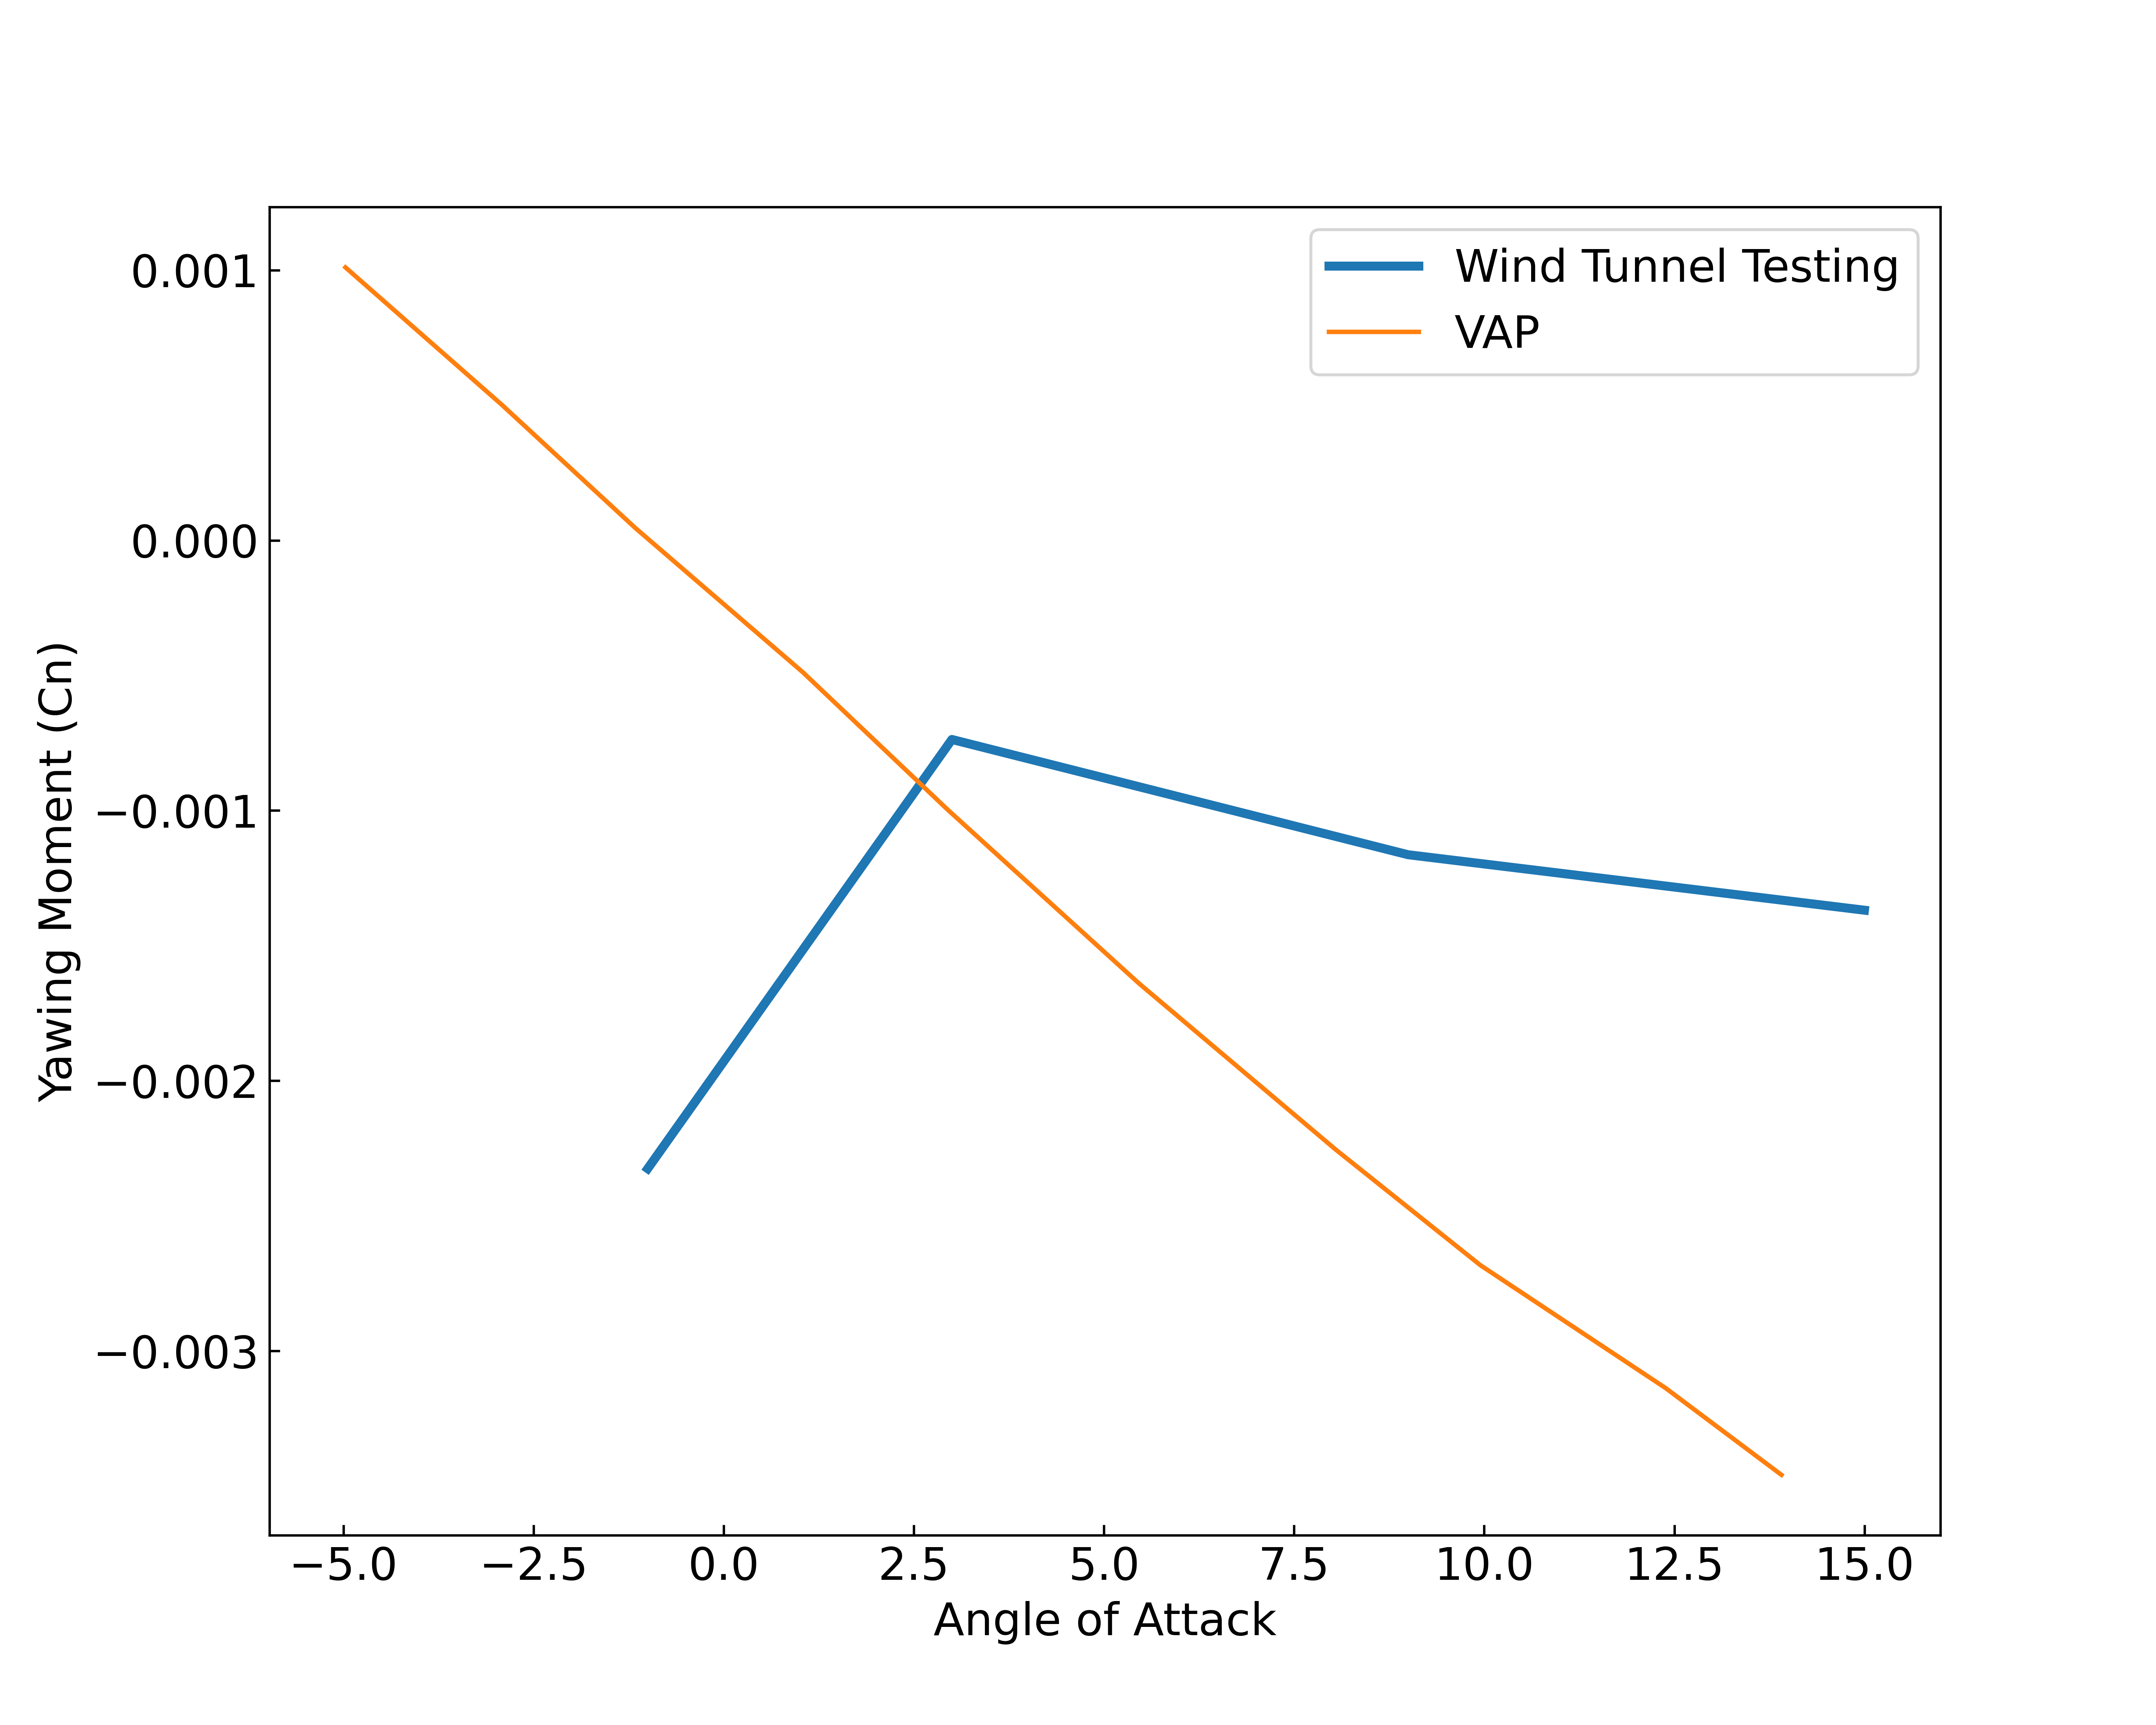
\includegraphics[width=\textwidth]{05_Results/VAP/noProp/Cn/10ms_11000RPM_Cn.png}
        \caption{Yawing Moment Coefficient at 10m/s airspeed and 11000RPM motor speed}
        \label{fig:VAP_noProp_Cm_10ms_11000}
    \end{subfigure}
    \begin{subfigure}[b]{0.467\textwidth}
        \centering
        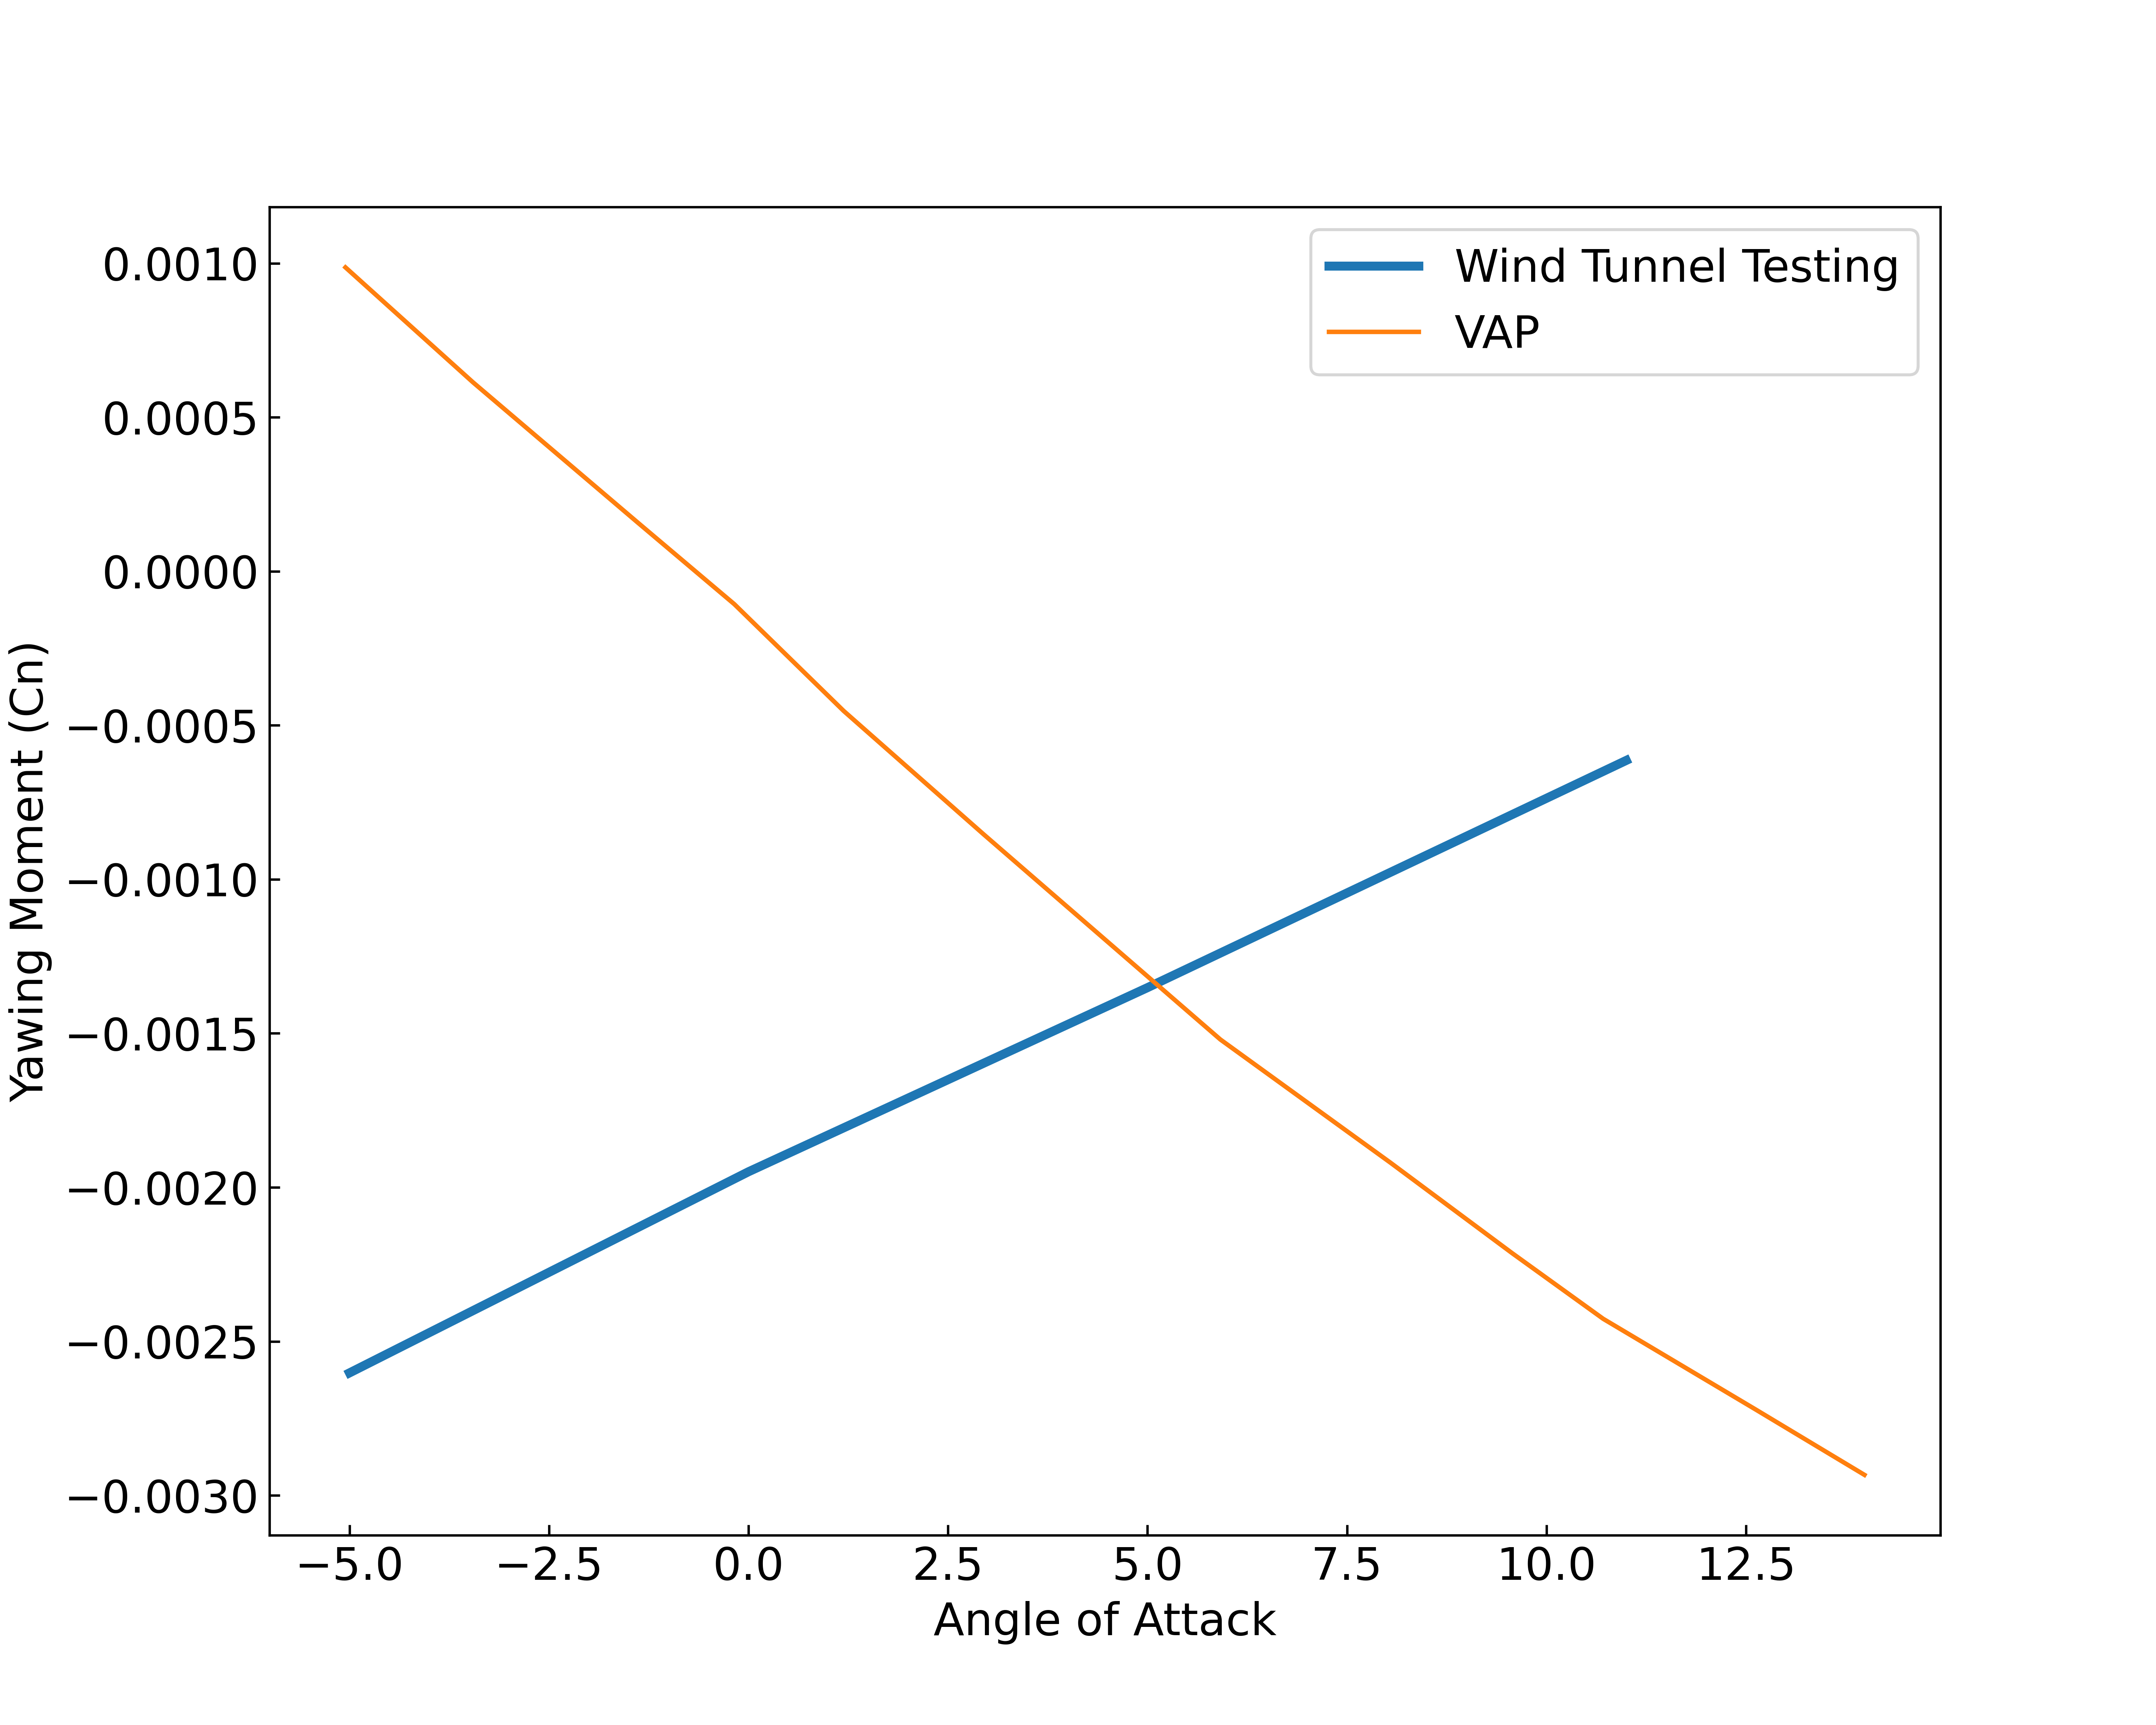
\includegraphics[width=\textwidth]{05_Results/VAP/noProp/Cn/20ms_6000RPM_Cn.png}
        \caption{Yawing Moment Coefficient at 20m/s airspeed and 6000RPM motor speed}
        \label{fig:VAP_noProp_Cm_20ms_6000}
    \end{subfigure}
    \begin{subfigure}[b]{0.467\textwidth}
        \centering
        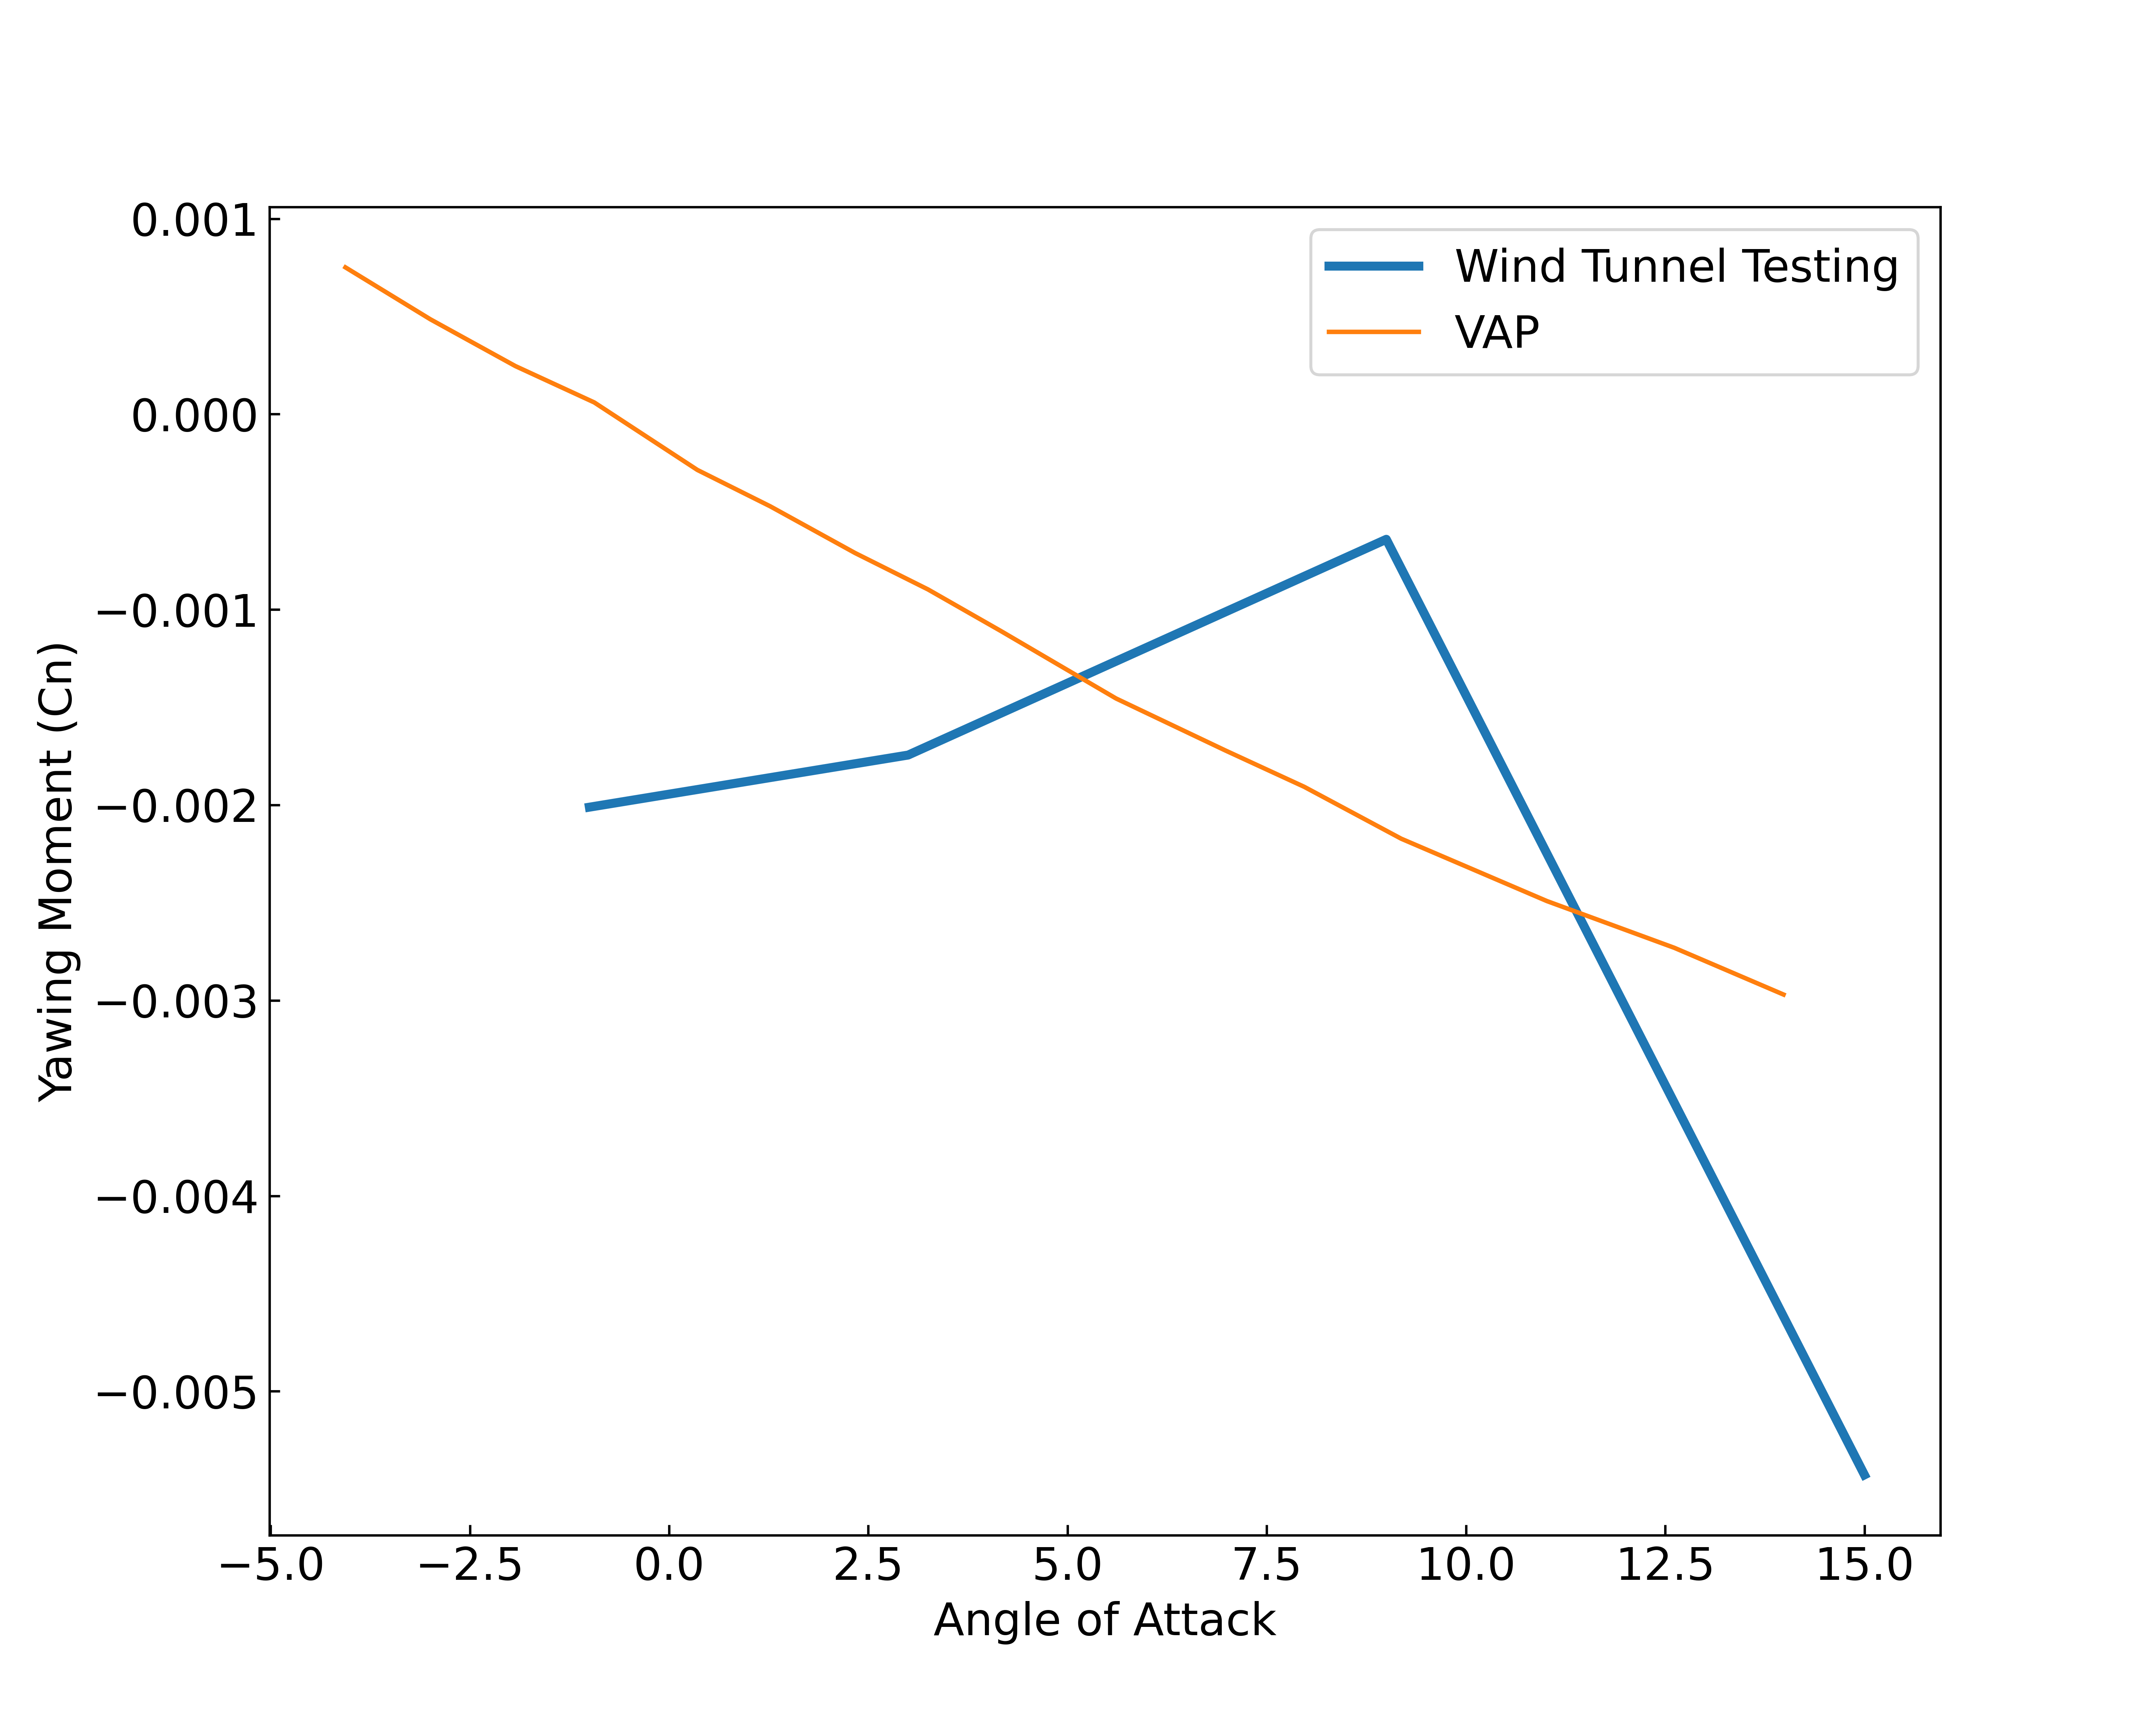
\includegraphics[width=\textwidth]{05_Results/VAP/noProp/Cn/20ms_11000RPM_Cn.png}
        \caption{Yawing Moment Coefficient at 20m/s airspeed and 11000RPM motor speed}
        \label{fig:VAP_noProp_Cm_20ms_11000}
    \end{subfigure}
\end{figure}



\subsubsection{Tractor Configuration}


\begin{figure}[H]
    \centering
    \begin{subfigure}[b]{0.467\textwidth}
        \centering
        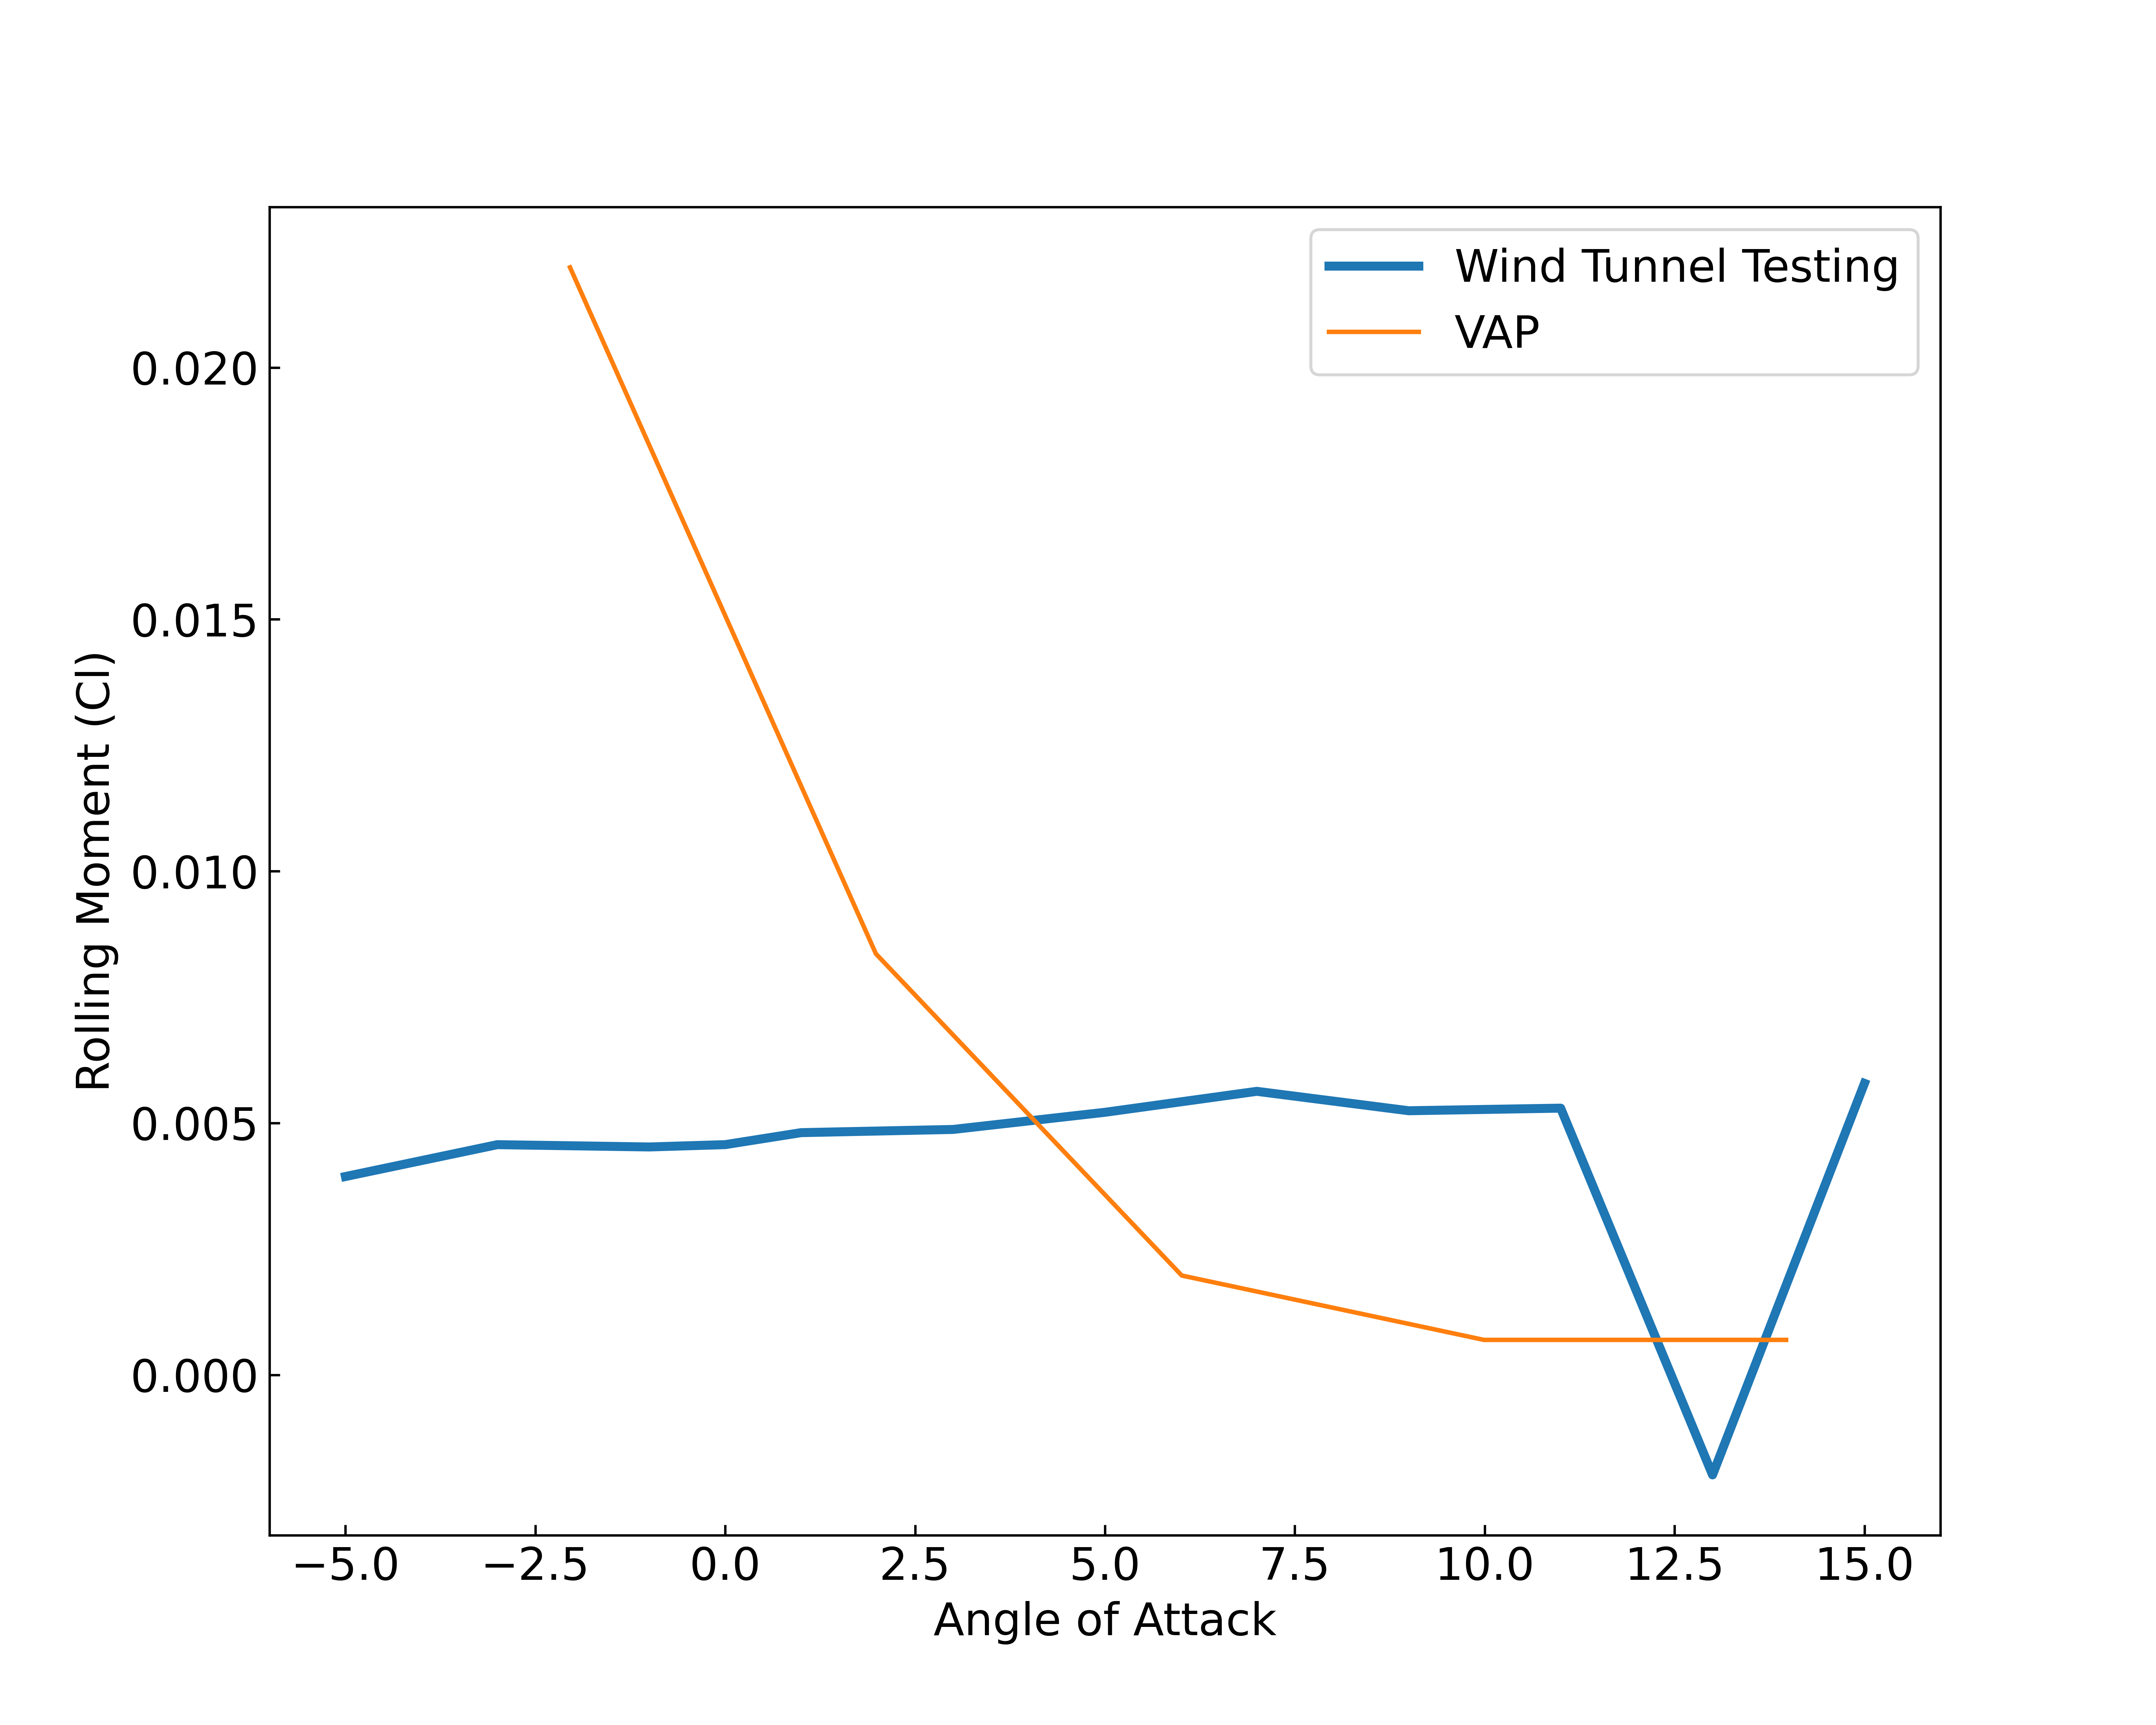
\includegraphics[width=\textwidth]{05_Results/VAP/tractor/Cl/10ms_6000RPM_Cl.png}
        \caption{Rolling Moment Coefficient at 10m/s airspeed and 6000RPM motor speed}
        \label{fig:VAP_Cl_10ms_6000}
    \end{subfigure}
    \begin{subfigure}[b]{0.467\textwidth}
        \centering
        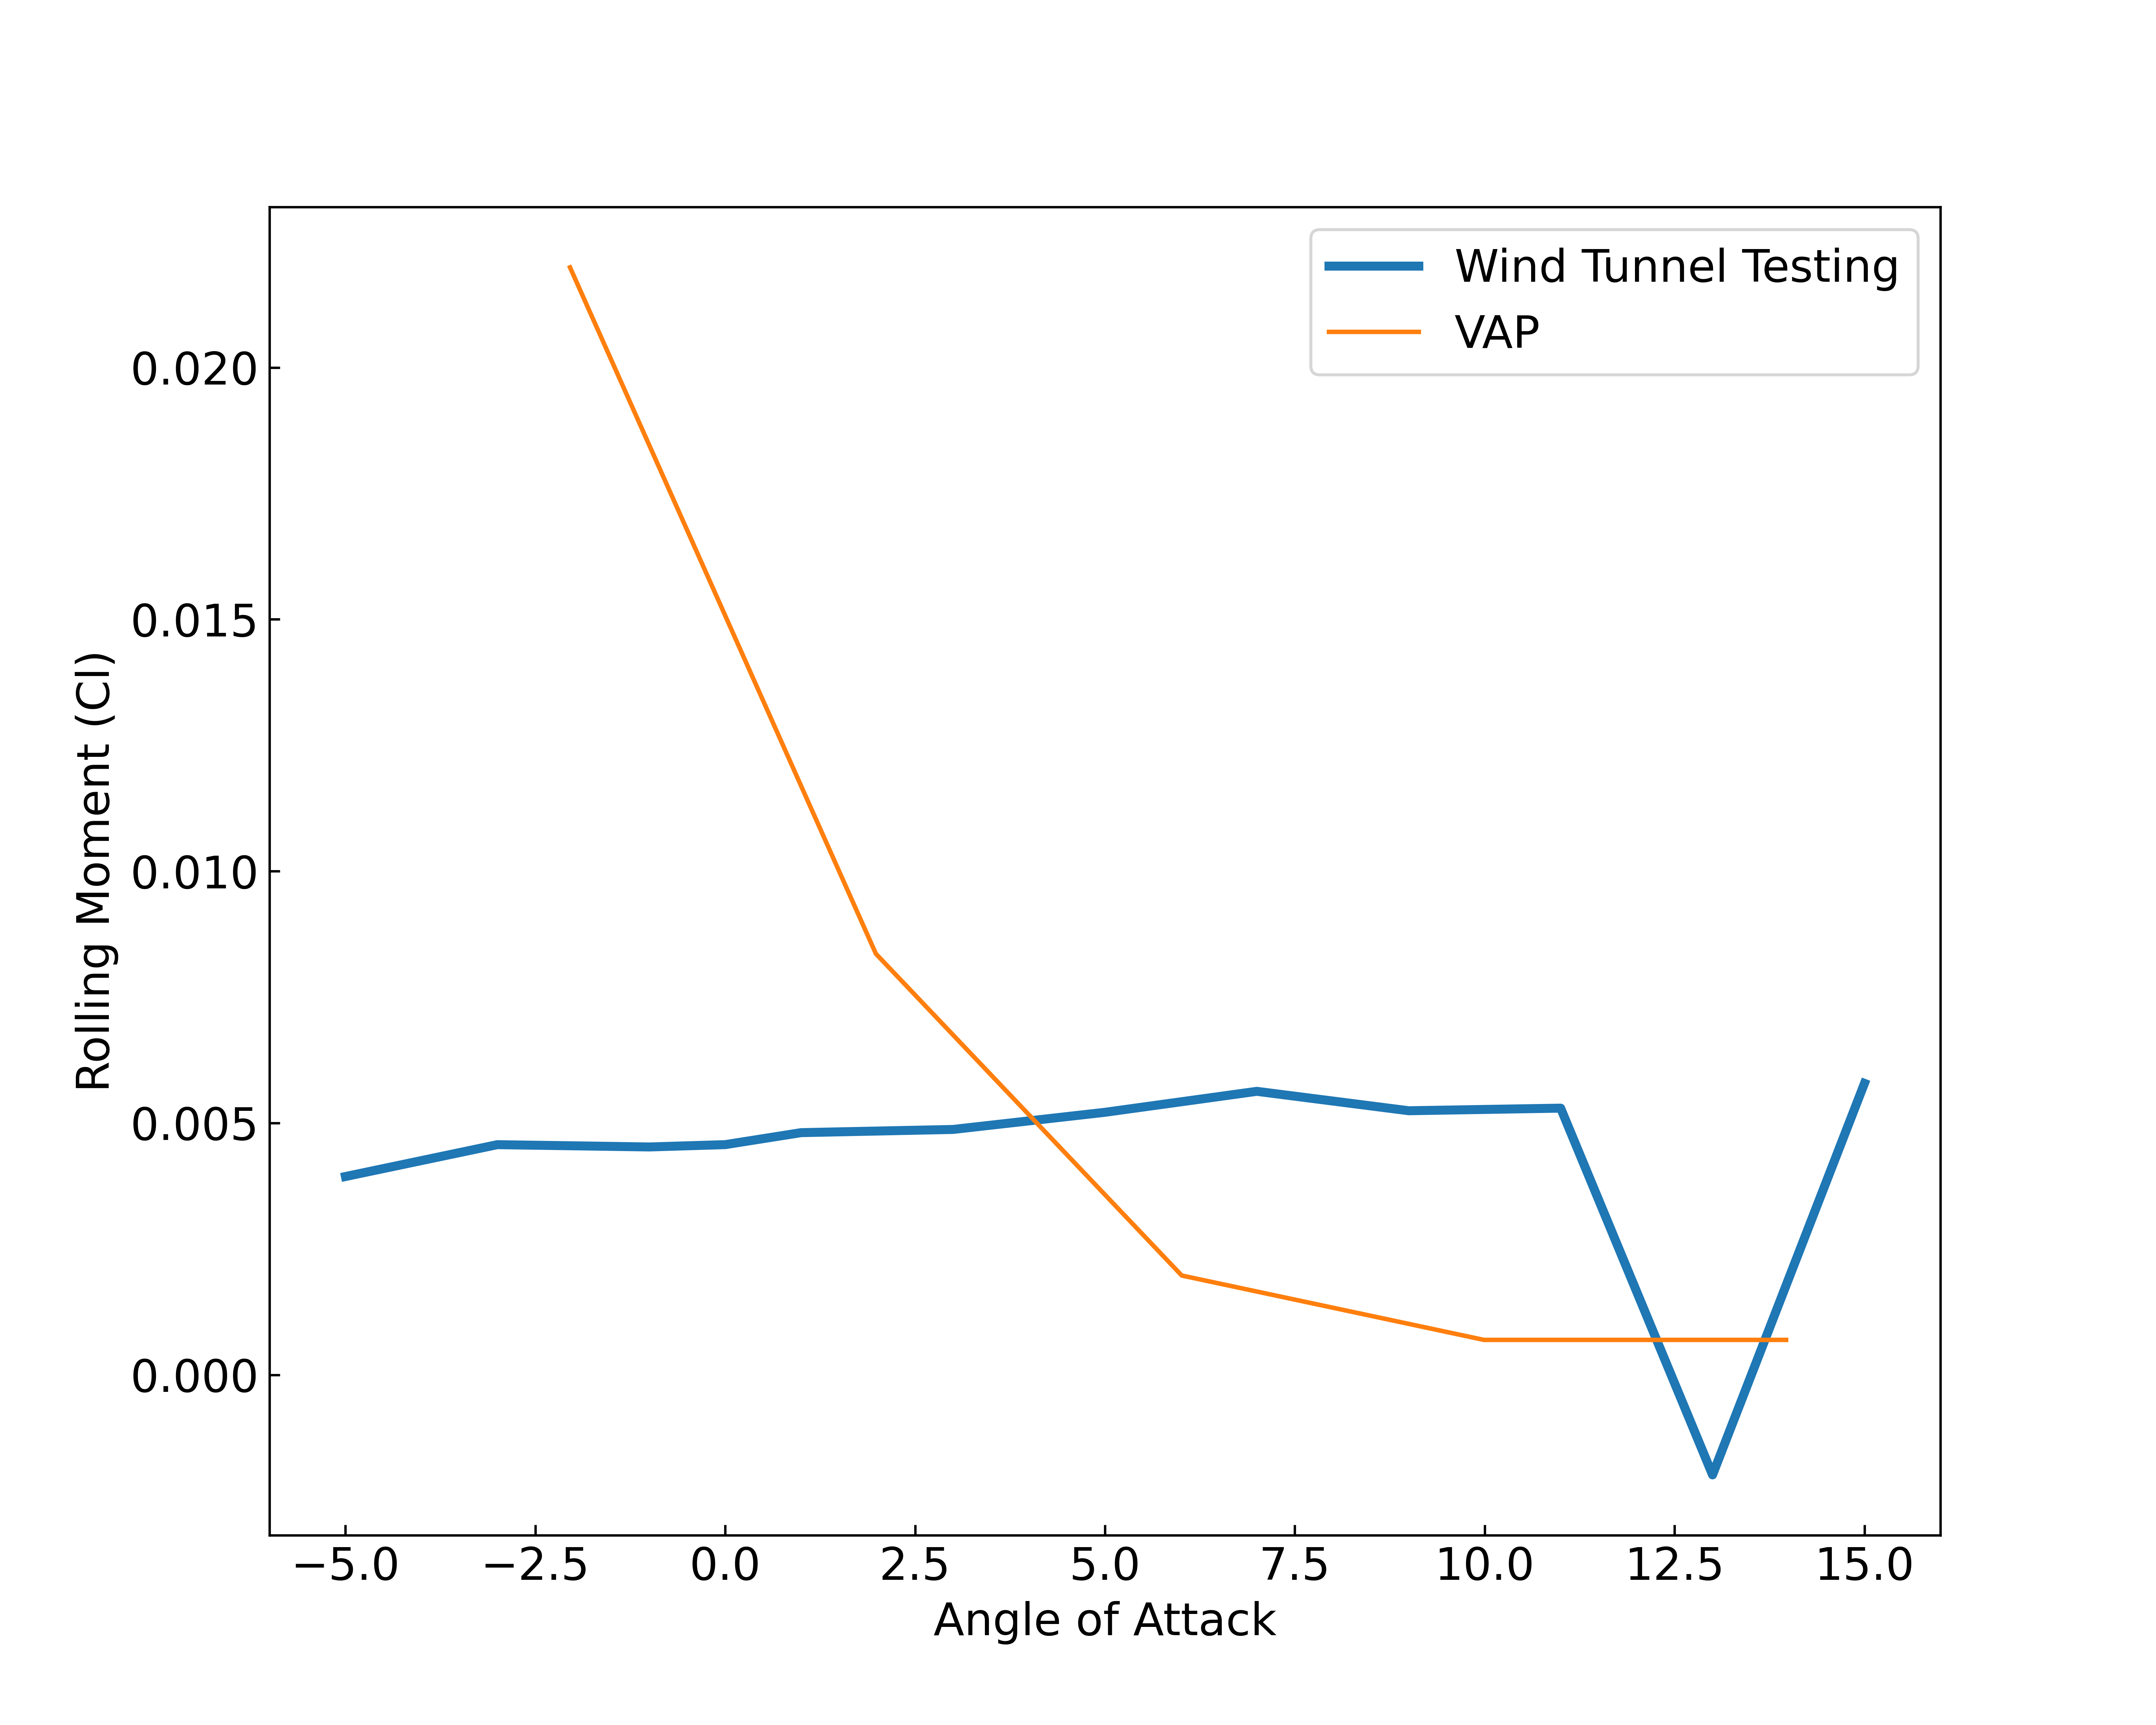
\includegraphics[width=\textwidth]{05_Results/VAP/tractor/Cl/10ms_6000RPM_Cl.png}
        \caption{Rolling Moment Coefficient at 10m/s airspeed and 11000RPM motor speed}
        \label{fig:Missing2}
    \end{subfigure}
    \begin{subfigure}[b]{0.467\textwidth}
        \centering
        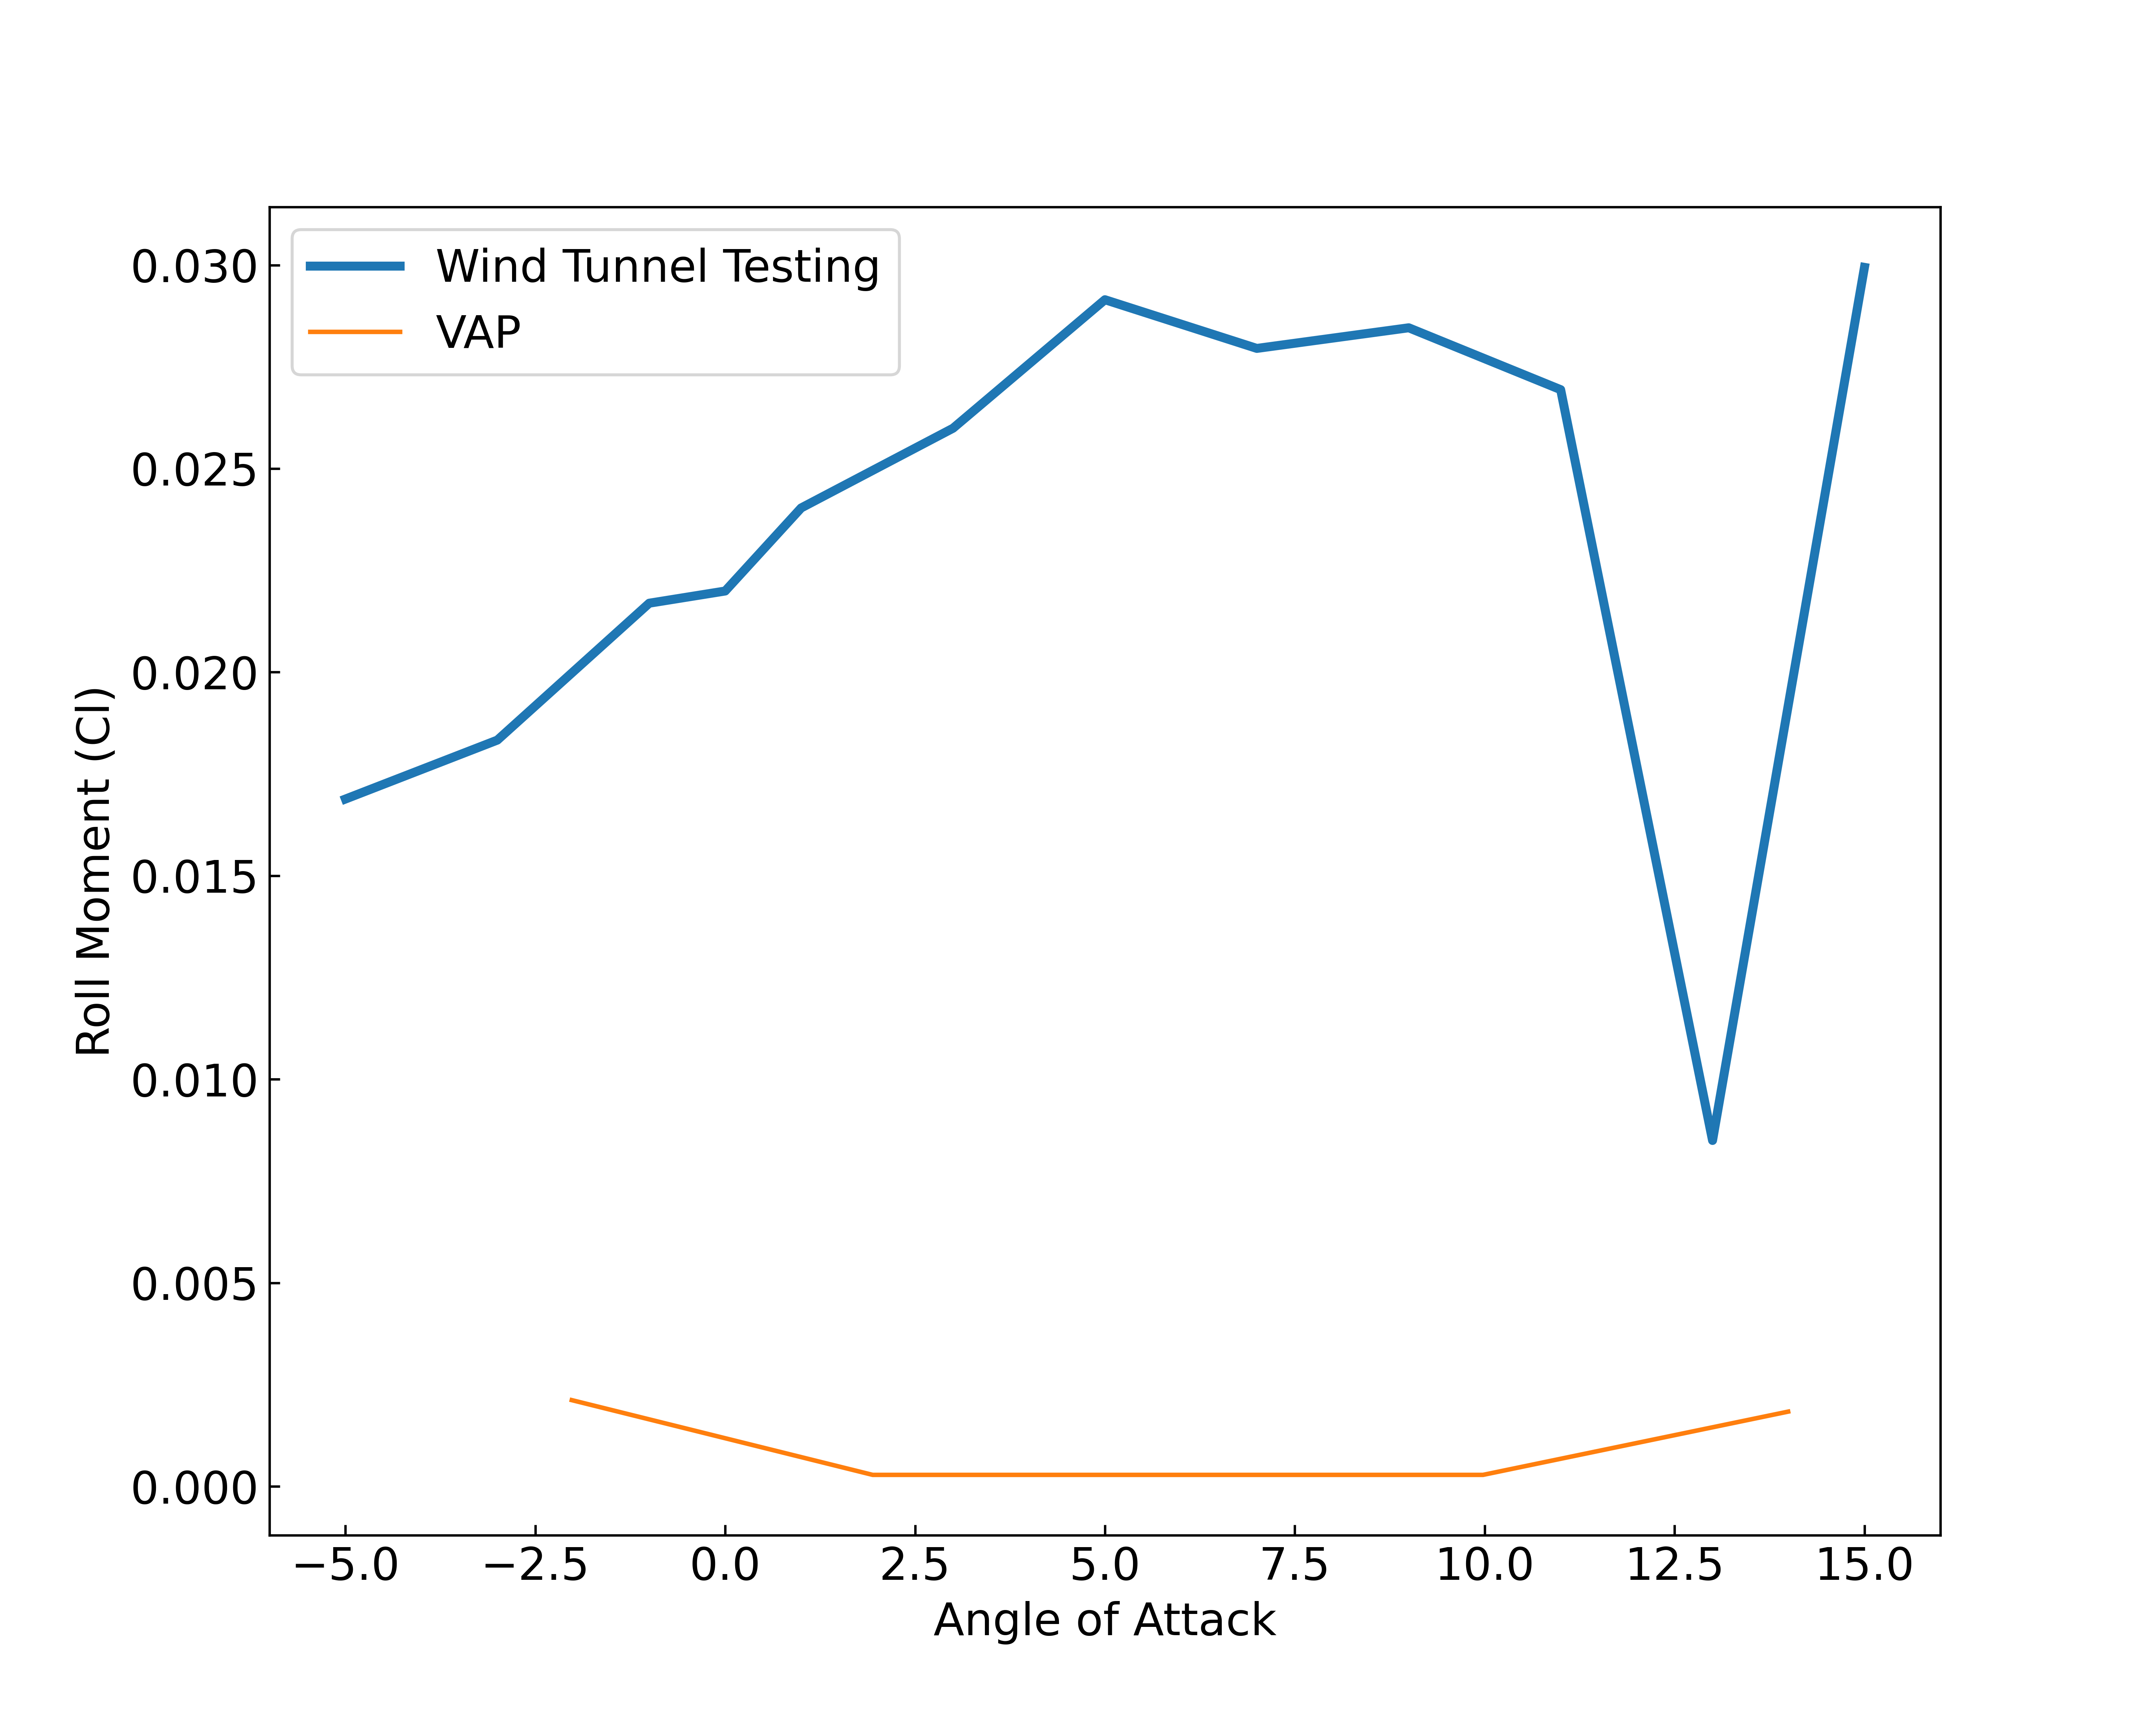
\includegraphics[width=\textwidth]{05_Results/VAP/tractor/Cl/20ms_6000RPM_Cl.png}
        \caption{Rolling Moment Coefficient at 20m/s airspeed and 6000RPM motor speed}
        \label{fig:VAP_Cl_20ms_6000}
    \end{subfigure}
    \begin{subfigure}[b]{0.467\textwidth}
        \centering
        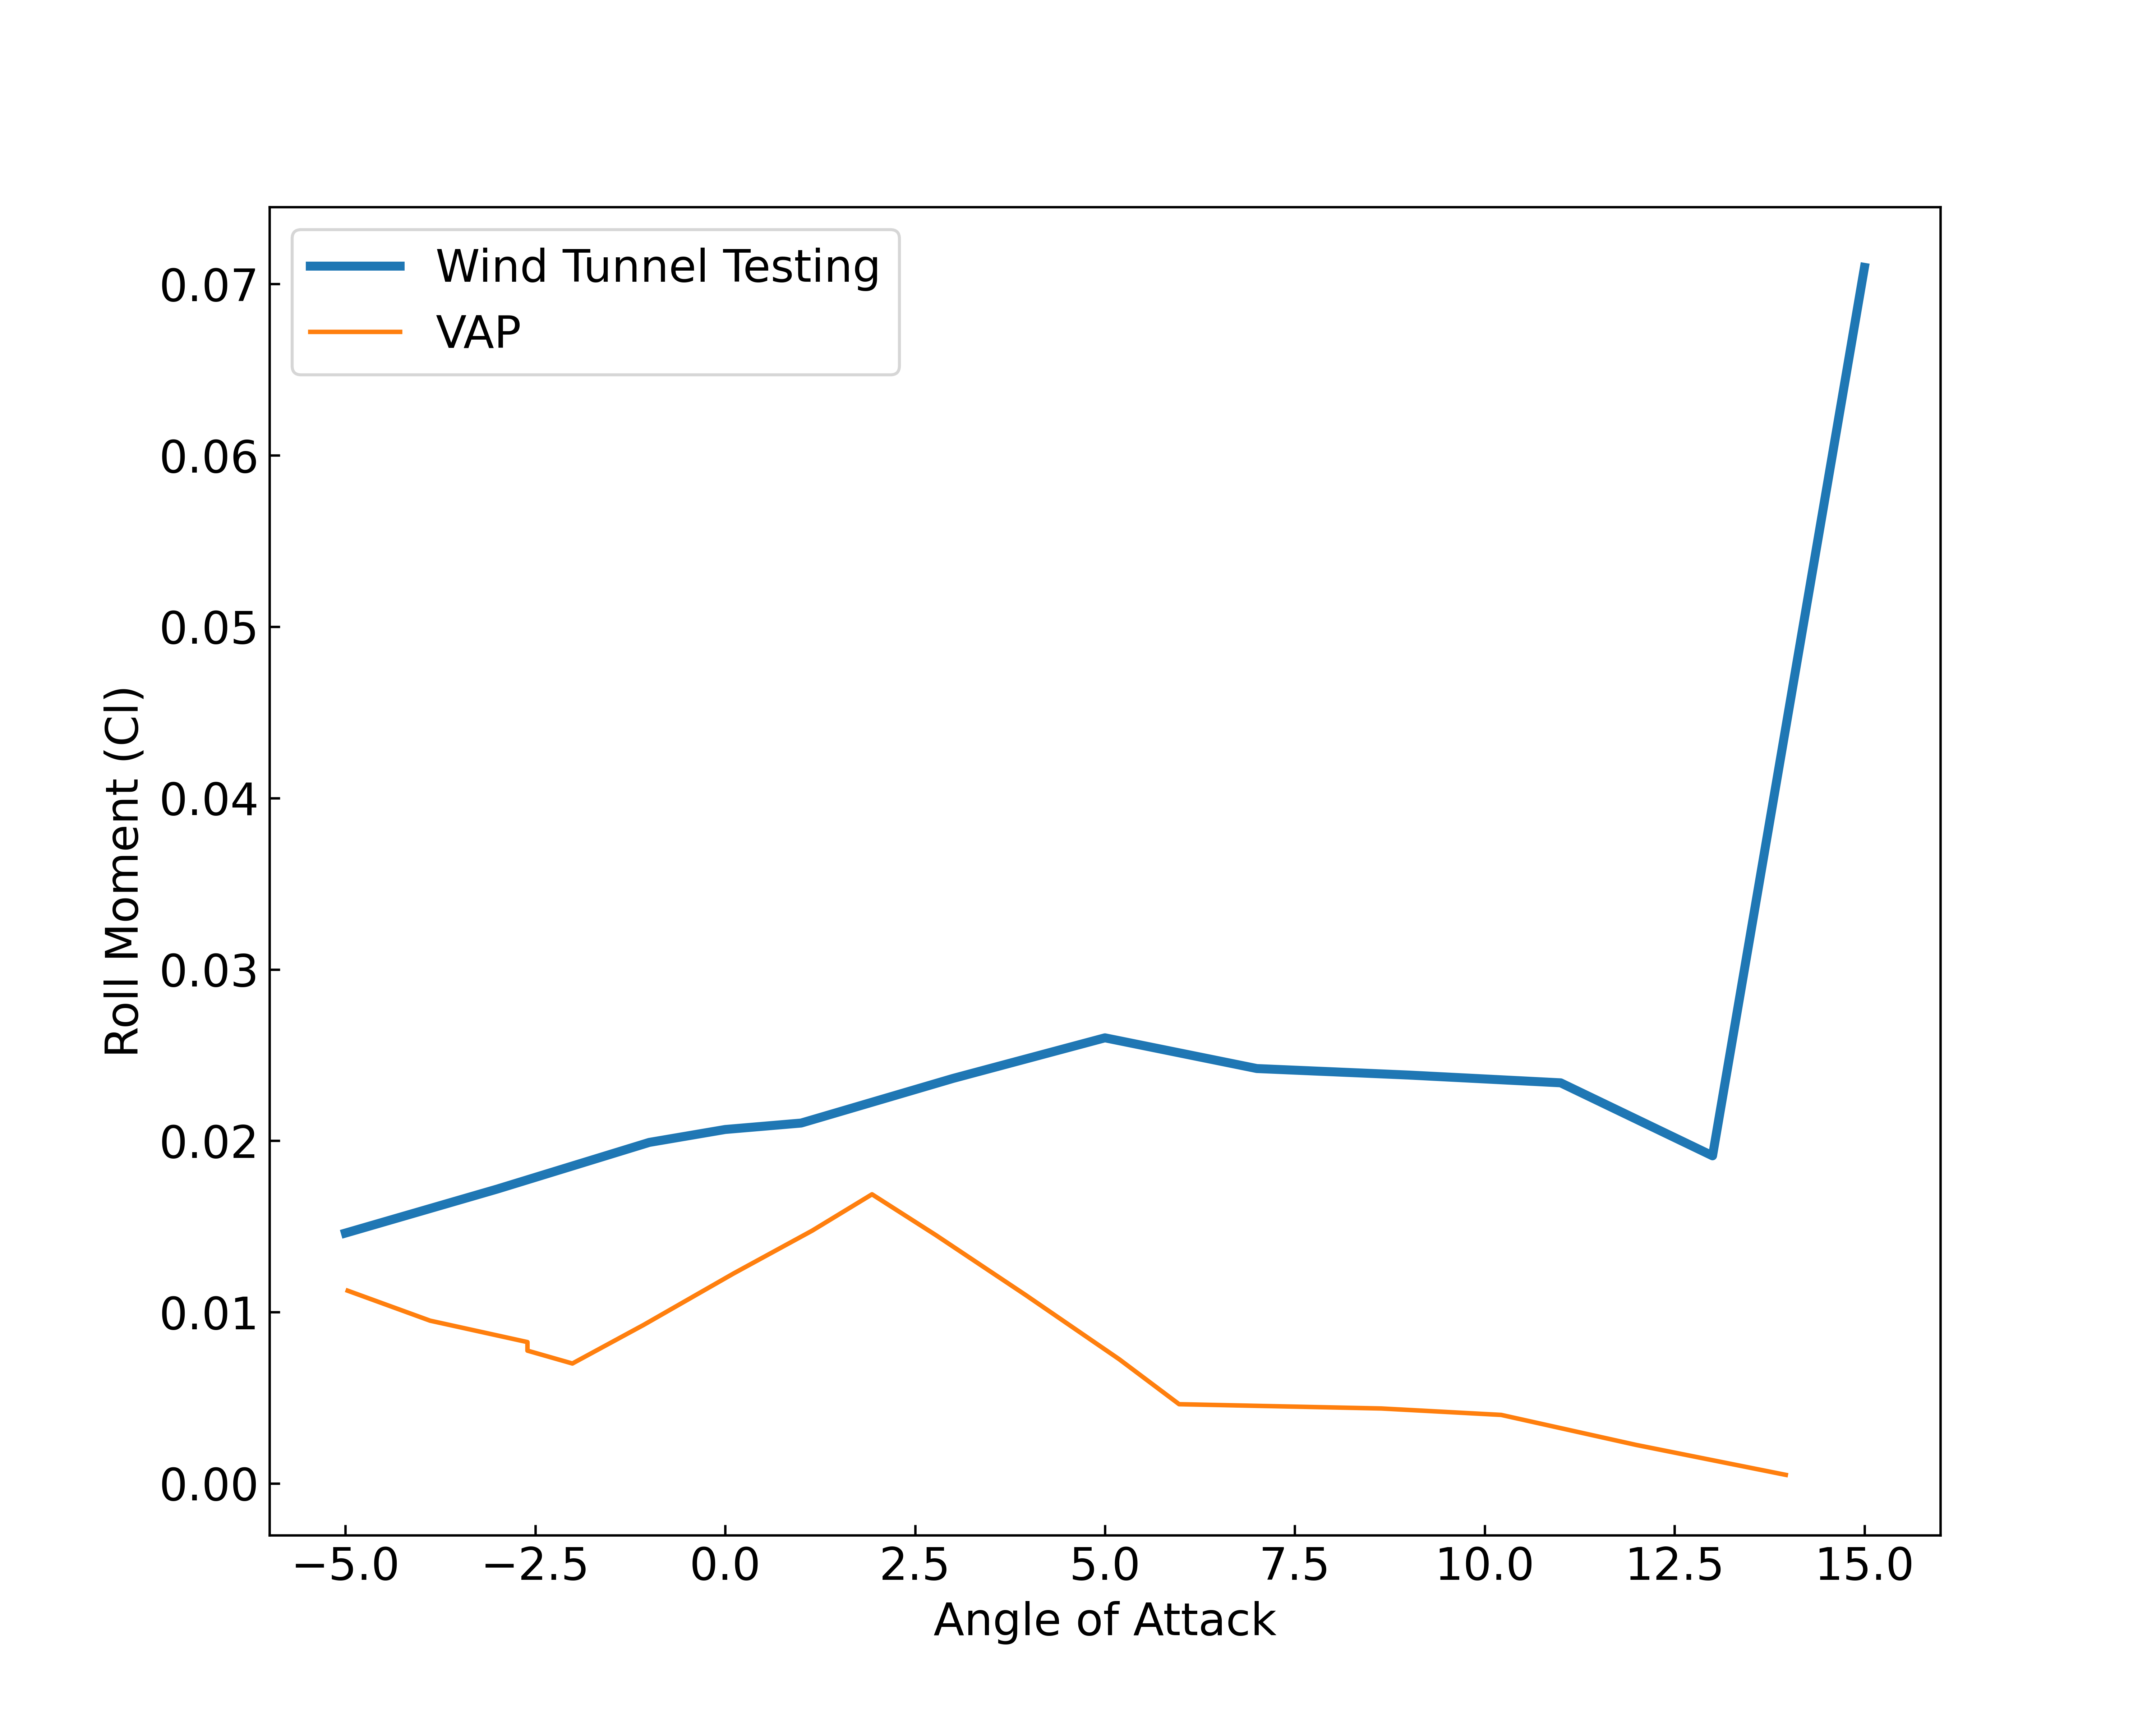
\includegraphics[width=\textwidth]{05_Results/VAP/tractor/Cl/20ms_11000RPM_Cl.png}
        \caption{Rolling Moment Coefficient at 20m/s airspeed and 11000RPM motor speed}
        \label{fig:VAP_Cl_20ms_11000}
    \end{subfigure}
\end{figure}


\begin{figure}[H]
    \centering
    \begin{subfigure}[b]{0.467\textwidth}
        \centering
        \includegraphics[width=\textwidth]{05_Results/VAP/tractor/Cm/10ms_6000RPM_Cm.png}
        \caption{Pitching Moment Coefficient at 10m/s airspeed and 6000RPM motor speed}
        \label{fig:VAP_Cm_10ms_6000}
    \end{subfigure}
    \begin{subfigure}[b]{0.467\textwidth}
        \centering
        \includegraphics[width=\textwidth]{05_Results/VAP/tractor/Cm/10ms_11000RPM_Cm.png}
        \caption{Pitching Moment Coefficient at 10m/s airspeed and 11000RPM motor speed}
        \label{fig:VAP_Cm_10ms_11000}
    \end{subfigure}
    \begin{subfigure}[b]{0.467\textwidth}
        \centering
        \includegraphics[width=\textwidth]{05_Results/VAP/tractor/Cm/20ms_6000RPM_Cm.png}
        \caption{Pitching Moment Coefficient at 20m/s airspeed and 6000RPM motor speed}
        \label{fig:VAP_Cm_20ms_6000}
    \end{subfigure}
    \begin{subfigure}[b]{0.467\textwidth}
        \centering
        \includegraphics[width=\textwidth]{05_Results/VAP/tractor/Cm/20ms_11000RPM_Cm.png}
        \caption{Pitching Moment Coefficient at 20m/s airspeed and 11000RPM motor speed}
        \label{fig:VAP_Cm_20ms_11000}
    \end{subfigure}
\end{figure}



\begin{figure}[H]
    \centering
    \begin{subfigure}[b]{0.467\textwidth}
        \centering
        \includegraphics[width=\textwidth]{05_Results/VAP/tractor/Cn/10ms_11000RPM_Cn.png}
        \caption{Yawing Moment Coefficient at 10m/s airspeed and 6000RPM motor speed}
        \label{fig:VAP_Cn_10ms_6000}
    \end{subfigure}
    \begin{subfigure}[b]{0.467\textwidth}
        \centering
        \includegraphics[width=\textwidth]{05_Results/VAP/tractor/Cn/10ms_11000RPM_Cn.png}
        \caption{Yawing Moment Coefficient at 10m/s airspeed and 11000RPM motor speed}
        \label{fig:Missing3}
    \end{subfigure}
    \begin{subfigure}[b]{0.467\textwidth}
        \centering
        \includegraphics[width=\textwidth]{05_Results/VAP/tractor/Cn/20ms_6000RPM_Cn.png}
        \caption{Yawing Moment Coefficient at 20m/s airspeed and 6000RPM motor speed}
        \label{fig:VAP_Cn_20ms_6000}
    \end{subfigure}
    \begin{subfigure}[b]{0.467\textwidth}
        \centering
        \includegraphics[width=\textwidth]{05_Results/VAP/tractor/Cn/20ms_11000RPM_Cn.png}
        \caption{Yawing Moment Coefficient at 20m/s airspeed and 11000RPM motor speed}
        \label{fig:VAP_Cn_20ms_11000}
    \end{subfigure}
\end{figure}


\subsubsection{Pusher Configuration}




\section{Discussion}